
%%%%%%%%%%%%%%%%%%%%%%%%%%%%%%%%%%%%%%%%%%%%%%%%%%%%%%%%%%%%%%%
%
%     filename  = "thesis_tjp.tex",
%     date      = "18/09/2013",
%     authors   = "Tara Jill Parkin",
%     copyright = "Tara Jill Parkin",
%     address   = "Physics & Astronomy,
%                  ABB, 245C
%                  McMaster University,
%                  Hamilton, ON,
%                  CANADA",
%     telephone = "",
%     email     = "parkintj@mcmaster.ca",
%
%%%%%%%%%%%%%%%%%%%%%%%%%%%%%%%%%%%%%%%%%%%%%%%%%%%%%%%%%%%%%%%

% This is the beginning of the end of my PhD!!!

%\documentclass[twoside,phd]{macthesis}
\documentclass[twoside,letterpaper,phd]{macthesis}
%%%%%%%%%%%%%%%%%%%%%%%%%%%%
% Packages we like to use. %
%%%%%%%%%%%%%%%%%%%%%%%%%%%%
\usepackage{fancyhdr}
\pagestyle{fancy}
\usepackage{deluxetable}
\usepackage{natbib} % \citet,\citep
\usepackage{aastex_hack} % Taken from: http://casa.colorado.edu/~danforth/comp/tex/thesistex.html
\usepackage{rotating}
\usepackage{lscape}

\usepackage{amsfonts}
\usepackage{amsmath}
\usepackage{amssymb}
\usepackage{amsthm}
\usepackage{exscale}
\usepackage[mathscr]{eucal}
\usepackage{bm}
\usepackage{eqlist} % Makes for a nice list of symbols.

\usepackage{graphicx}

\usepackage{epigraph}
\usepackage{lettrine}
\usepackage{keyval}

\usepackage[dvipsnames]{color}
\usepackage{times}
\usepackage{acronym}
\usepackage{subfig}
%\documentstyle[fancyhdr]
%\usepackage{tabular}
%\DeclareGraphicsExtensions{.pdf, .jpg}


\usepackage{multirow}

%%%%%%%%%%%%%%%%%%%%%%%%
% Setting for fncychap %
%%%%%%%%%%%%%%%%%%%%%%%%
% Comment out or remove the next two lines and you will get
% the standard LaTeX chapter titles. We like these A LOT
% better.
\usepackage[Lenny]{fncychap}
\ChTitleVar{\Huge\sffamily\bfseries}


%%%%%%%%%%%%%%%%%%%%%%%%%%%%%%%%%%%%
% SPECIAL SYMBOLS AND NEW COMMANDS %
%%%%%%%%%%%%%%%%%%%%%%%%%%%%%%%%%%%%
%\input{SupplementaryMaterial/UserDefinedCommands}


%%%%%%%%%%%%%%%%%%%%%%%%%%%%%%%%%%%%%%%%%
% Renewed Float Parameters              %
% (Makes floats fit better on the page) %
%%%%%%%%%%%%%%%%%%%%%%%%%%%%%%%%%%%%%%%%%
\renewcommand{\floatpagefraction}{0.85}
\renewcommand{\topfraction}      {0.85}
\renewcommand{\bottomfraction}   {0.85}
\renewcommand{\textfraction}     {0.15}



% Alter some LaTeX defaults for better treatment of figures:
% See p.105 of "TeX Unbound" for suggested values.
% See pp. 199-200 of Lamport's "LaTeX" book for detail
%   General parameters, for ALL pages:
\renewcommand{\topfraction}{0.9}	% max fraction of floats at top
\renewcommand{\bottomfraction}{0.8}	% max fraction of floats at bottom
%   Parameters for TEXT pages (not float pages):
\setcounter{topnumber}{2}
\setcounter{bottomnumber}{2}
\setcounter{totalnumber}{4}     % 2 may work better
\setcounter{dbltopnumber}{2}    % for 2-column pages
\renewcommand{\dbltopfraction}{0.9}	% fit big float above 2-col. text
\renewcommand{\textfraction}{0.07}	% allow minimal text w. figs
%   Parameters for FLOAT pages (not text pages):
\renewcommand{\floatpagefraction}{0.7}	% require fuller float pages
% N.B.: floatpagefraction MUST be less than topfraction !!
\renewcommand{\dblfloatpagefraction}{0.7}	% require fuller float pages

% ----------------------------------------------------------- %

%%%%%%%%%%%%%%%%
% FRONT-MATTER %
%%%%%%%%%%%%%%%%
% Title
\title{Unlocking the Properties of the Interstellar Medium of Centaurus~A and M51}
\halftitle{THE INTERSTELLAR MEDIUM OF CENTAURUS A AND M51}
% Author and Department
\author{Tara Jill Parkin, B.Sc., M.Sc.}
\dept{Physics \& Astronomy}
% the degree will be conferred on this date
\degreedate{November 2013}
\copyrightyear{2013}


\documenttype{Thesis}

% This will generally be The Graduate School, though you can
% put anything in here to suit your needs.
\submittedto{School of Graduate Studies}


%%%%%%%%%%%%%%%%%%
% Signatory Page %
%%%%%%%%%%%%%%%%%%
% You can have up to 7 committee members, i.e., one advisor
% and up to 6 readers.
%
% Begin by specifying the number of readers.
\numberofreaders{2}


\advisor[Thesis Advisor]
        {Dr. Christine Wilson}
        {Professor, McMaster University}

\readerone[Committee Member]
        {Dr. Laura Parker}
        {Professor, McMaster University}

\readertwo[Committee member]
          {Dr. James Wadsley}
          {Professor, McMaster University}

%\readerthree[Committee member, Chair of Committee]
%          {Dr.???}
%          {Professor, McMaster University}


% Makes use of LaTeX's include facility. Add as many chapters
% and appendices as you like.


%\includeonly{%
%Ch1/ch1,%
%Ch2/ch2,%
%Ch3/ch3,%
%Ch4/ch4,%
%Ch5/ch5,%
%}
%Chapter-6/Chapter-6,%
%Chapter-7/Chapter-7,%
%Appendix-A/Appendix-A,%
%Appendix-B/Appendix-B%
%}

%%%%%%%%%%%%%%%%%
% THE BEGINNING %
%%%%%%%%%%%%%%%%%

\begin{document}
\parindent=0.5in

%\graphicspath{{Figure/}} define figure search path

%%%%%%%%%%%%%%%%%%%%%%%%
% Preliminary Material %
%%%%%%%%%%%%%%%%%%%%%%%%
% This command is needed to properly set up the frontmatter.
\frontmatter


%%%%%%%%%%%%%%%%%%%%%%%%%%%%%%%%%%%%%%%%%%%%%%%%%%%%%%%%%%%%%%
% IMPORTANT
%
% The following commands allow you to include all the
% frontmatter in your thesis. If you don't need one or more of
% these items, you can comment it out. Most of these items are
% actually required by the Grad School -- see the Thesis Guide
% for details regarding what is and what is not required for
% your particular degree.
%%%%%%%%%%%%%%%%%%%%%%%%%%%%%%%%%%%%%%%%%%%%%%%%%%%%%%%%%%%%%%
% !!! DO NOT CHANGE THE SEQUENCE OF THESE ITEMS !!!
%%%%%%%%%%%%%%%%%%%%%%%%%%%%%%%%%%%%%%%%%%%%%%%%%%%%%%%%%%%%%%

% Generates the signature page. This is not bound with your
% thesis.
%\macsigpage


% Generates the committee page -- this is bound with your
% thesis. If this is an baccalaureate honors thesis, then
% comment out this line.
%\maccommitteepage


% Generates the title page based on info you have provided
% above.
\mactitlepage


% Generate the descriptive note page: Short-title page
\descriptivenote{SupplementaryMaterial/DescriptiveNote}


% Generates the abstract. The argument should point to the
% file containing your abstract.
\thesisabstract{SupplementaryMaterial/Abstract}

% Generates the Epigraph/Dedication. The first argument should
% point to the file containing your Epigraph/Dedication and
% the second argument should be the title of this page.
\thesisdedication{SupplementaryMaterial/Dedication}{}

\thesiscoauthorship{SupplementaryMaterial/Co-Authorship}

\thesisacknowledgments{SupplementaryMaterial/Acknowledgments}

\thesisepigraph{SupplementaryMaterial/Epigraph}


% Generates the Table of Contents
\thesistableofcontents



% Generates the List of Figures
\thesislistoffigures



% Generates the List of Tables
\thesislistoftables

% Generates the List of Symbols. The argument should point to
% the file containing your List of Symbols.
\thesislistofsymbols{SupplementaryMaterial/ListOfSymbols}

% Generates the Acknowledgments. The argument should point to
% the file containing your Acknowledgments.
%\thesisacknowledgments{SupplementaryMaterial/Acknowledgments}





%%%%%%%%%%%%%%%%%%%%%%%%%%%%%%%%%%%%%%%%%%%%%%%%%%%%%%
% This command is needed to get the main part of the %
% document going.                                    %
%%%%%%%%%%%%%%%%%%%%%%%%%%%%%%%%%%%%%%%%%%%%%%%%%%%%%%

%\thesisepigraph{SupplementaryMaterial/Epigraph}


\thesismainmatter

%%%%%%%%%%%%%%%%%%%%%%%%%%%%%%%%%%%%%%%%%%%%%%%%%%
% This is an AMS-LaTeX command to allow breaking %
% of displayed equations across pages. Note the  %
% closing the "}" just before the bibliography.  %
%%%%%%%%%%%%%%%%%%%%%%%%%%%%%%%%%%%%%%%%%%%%%%%%%%
\allowdisplaybreaks{
%
%%%%%%%%%%%%%%%%%%%%%%
% THE ACTUAL CONTENT %
%%%%%%%%%%%%%%%%%%%%%%
% Chapters
%\begin{singlespace}
\begin{doublespace}
\pagestyle{fancy}
\headheight 20pt
\lhead{Ph.D. Thesis --- T.~J. Parkin }
\rhead{McMaster - Physics \& Astronomy}
\chead{}
\lfoot{}
\cfoot{\thepage}
\rfoot{}
\renewcommand{\headrulewidth}{0.1pt}
\renewcommand{\footrulewidth}{0.1pt}

\chapter{Introduction} \label{chapter1} 

\thispagestyle{fancy} 
The night sky is full of stars, the moon and planets, galaxies and a variety of other galactic objects.  Historically, our perspective of these objects was limited to what we could see with our eyes or through an optical telescope, which covers a small range of the electromagnetic spectrum.  But our perspective changed in the 1930s when Karl G. Jansky discovered radio emission originating in the centre of the Milky Way Galaxy \citep{1933Natur.132...66J}, thus opening the door to radio astronomy and a new part of the electromagnetic spectrum.  Since then, numerous ground- and spaced-based observatories have been built to probe the sky across the entire electromagnetic spectrum, and we have come to the realisation that the Universe and the objects within it are much more complex, rich and diverse than might have been suggested by optical observations alone.  Thus, to fully understand the physics behind the phenomena we observe, it is necessary to conduct a multiwavelength study of each object.

Galaxies themselves are extremely rich objects.  They are large gravitationally bound systems that fall into three broad morphological types: spiral/disk galaxies, elliptical galaxies and irregular types.  Each galaxy is enriched with dark matter, stars and the stuff between them, which we call the interstellar medium (ISM).  The ISM comprises gas and dust in a variety of phases, such as molecular clouds, regions of ionised gas known as H~\textsc{ii} regions, or diffuse gas, and is the location of many physical processes including star formation, dust grain formation, metal enrichment, and energy transport, all of which rely on the evolution of stars and stellar systems \citep{1995ASPC...73....3T}.  

An important wavelength regime to utilise for probing the ISM is that of the infrared and submillimetre, which traces thermal emission at dust temperatures typically less than $\sim$100~K  and gas temperatures of less than $10^{3}$~K \citep{2005pcim.book.....T}.  Ranging from approximately 2~$\mu$m to 1~mm, a significant fraction of a star-forming galaxy's total flux is emitted at these wavelengths, as shown by the spectral energy distribution (SED) for the centre of M51 in Figure~\ref{fig:M51_sed}.  At near-infrared wavelengths, the continuum emission is dominated by older stellar populations.  In the mid-infrared wavebands a small amount of radiation comes from the tail end of the stellar SEDs, while the rest of the emission comes from stochastically heated hot dust grains (continuum), as well as polycyclic aromatic hydrocarbons (PAHs) and a number of atomic and molecular fine structure lines (spectral line emission) \citep[e.g.][]{2007ApJ...657..810D}.  Between the mid-infrared and the submillimetre the SED comprises emission primarily from dust grains.  However, a significant fraction of emission at these wavelengths also comes from atomic and molecular fine structure lines tracing the cool gas \citep{1999ApJ...527..795K}.  Comparing observations of the dust and gas emission at these wavelengths with models of dust SEDs \citep[e.g.][]{2001ApJ...549..215D,2003A&A...407..159G,2007ApJ...663..866D,2011A&A...536A..88G} and photon dominated region (PDR) models \citep[e.g.][]{1985ApJ...291..722T, 1990ApJ...358..116W, 1991ApJ...377..192H, 1999ApJ...527..795K, 2006ApJ...644..283K,2006A&A...451..917R} gives us insight into the physical properties of the ISM and star formation.

\begin{figure}[!h]
 \begin{center}
 \includegraphics[width=\columnwidth]{ch1/M51_SED_Mentuch2012.eps}
  \caption[Spectral energy distribution of the centre of M51]{The spectral energy distribution for the centre of M51.  Observed data are represented by the black dots while the best-fitting SED model flux at each corresponding waveband is shown by the open triangles.  The best-fitting stellar SED model is represented by the purple curve and the best-fitting dust SED model is shown in red.  The dust SED model is further subdivided into a PDR component and an underlying component shown as the orange dotted and dashed lines, respectively.  The green dashed line is a modified blackbody fit. \emph{Image credit: Adapted from Figure~4 of Mentuch Cooper, E.~et al., 2012, "Spatially resolved stellar, dust, and gas properties of the post-interacting Whirlpool system", The Astrophysical Journal, Volume 755, Issue 2, Article ID 165, 23pp.  Reproduced by permission of the American Astronomical Society.}
  \label{fig:M51_sed}}
 \end{center}
\end{figure}

The one major caveat of observing the sky in these wavebands is that they suffer from atmospheric effects, meaning much of the radiation is absorbed before it can be observed on the ground \citep[e.g.][]{2013MNRAS.430.2513H}.  Ground-based observatories located at high altitudes and in dry climates, such as the James Clerk Maxwell Telescope (JCMT) and the Atacama Large Millimetre Array (ALMA), can partially observe the sky within select windows.  In Figure~\ref{fig:atmos_trans} we show the atmospheric transmission of submillimetre radiation as a function of wavelength (grey solid line) at the JCMT site at the summit of Mauna Kea, roughly 4000~m above sea level.  Also shown are the filter shapes of the two bands observed by the Submillimetre Common User Bolometer Array 2 (SCUBA-2) instrument mounted on the JCMT, 450~$\mu$m (blue) and 850~$\mu$m (red).  What is striking about this plot is that at wavelengths of less than about 600~$\mu$m, there are only two observable windows, where at most only about half of the radiation at these wavelengths is observed; emission at wavelengths in between these windows is completely unobservable by the JCMT.  The best solution to this problem is to build space-based observatories, which are capable of accessing emission across all wavelengths, or airborne observatories mounted on airplanes that are a compromise between ground-based and space-based observatories. 

\begin{figure}[!h]
 \begin{center}
 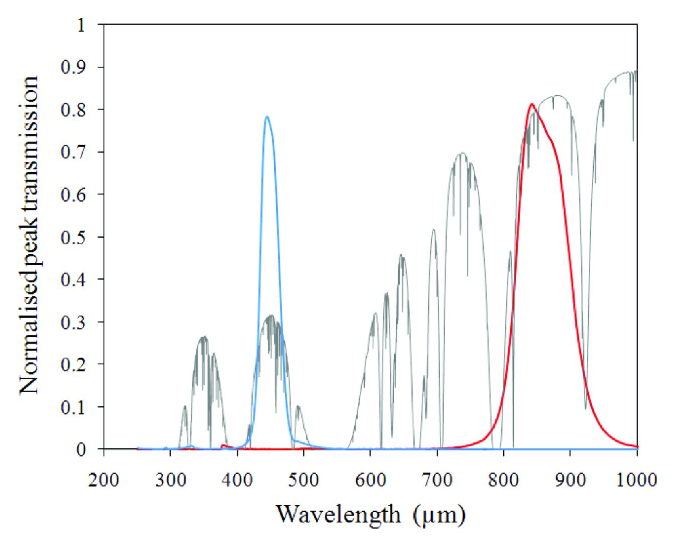
\includegraphics[width=\columnwidth]{ch1/Holland2013_transmission_plot.eps}
  \caption[Atmospheric transmission as a function of frequency at the summit of Mauna Kea]{A plot of the fraction of submillimetre emission that passes through the atmosphere as a function of wavelength at the summit of Mauna Kea, Hawaii (altitude approximately 4000~m).  The blue and red curves show the filter profiles of the 450 and 850~$\mu$m bands, respectively, of the SCUBA-2 instrument mounted on the JCMT.  \emph{Image credit: Figure~3 from Holland, W.~S.~et al., 2013, "SCUBA-2: The 10000 pixel bolometer camera on the James Clerk Maxwell Telescope", Monthly Notices of the Royal Astronomical Society, Volume 430, Issue 4, Pages 2513-2533.  Reproduced with permission from the Monthly Notices of the Royal Astronomical Society and Oxford University Press.}
  \label{fig:atmos_trans}}
 \end{center}
\end{figure}

%%%%%%%%%%%%% ISM
\section{The Interstellar Medium} \label{ism}
The interstellar medium (ISM) of a galaxy is a complex, multiphase environment, comprised primarily of gas and dust components and permeated by radiation at energies across much of the electromagnetic spectrum.  Its evolution with time is driven by the dynamics of the galaxy, and more importantly for the purposes of this thesis, star formation and subsequent feedback \citep{2005pcim.book.....T}.  Young star clusters rich in young, massive O and B stars provide a source of strong stellar winds and an outward flux of ionising radiation directed toward the surrounding gas and dust, impacting the physical characteristics of these components \citep{2007ARA&A..45..481Z}.  Furthermore, the violent death of these high-mass stars in supernova explosions deposits mechanical energy and material back into the ISM, which in turn recycles this matter into the next generation of stars.  We summarise the gas and dust components relevant to this thesis below.

\subsection{Interstellar Gas} \label{gas}
Interstellar gas permeates a galaxy and exists in a number of phases with a broad range of temperatures, and densities, and can be in both neutral and ionised states.  The bulk of the mass of a star-forming galaxy comprises hydrogen, both atomic (H~\textsc{i}) and molecular (H$_{2}$), though the relative contributions of each varies from galaxy to galaxy \citep{1989ApJ...347L..55Y,2002A&A...384...33B, 2009MNRAS.394.1857O}.  A wealth of atomic and molecular species make up the remaining fraction of gas.  Here we briefly describe the major components of the ISM and the typical ways to observe them.

The coldest gas is located within molecular clouds, the sites of star formation.  The temperature in these regions is very cold, typically 10~K \citep{1991ARA&A..29..581Y}, and the typical gas density is of the order $10^{2}$~cm$^{-3}$ \citep{2012arXiv1210.6990S}, which allows for the formation of molecules.  Molecular hydrogen comprises the majority of the gas in these clouds, followed by carbon monoxide (CO), the second most common molecule \citep[e.g.][]{1982ApJ...262..590F}.  In the densest regions other common molecular constituents include HCN, CS, HCO$^{+}$ and NH$_{3}$ \citep{2005pcim.book.....T,2007ARA&A..45..339B,2012arXiv1210.6990S}.  Star formation occurs in embedded cores within these clouds, where the conditions are different than the rest of the cloud.

Immediately surrounding regions of star formation are low density, ionised environments called H~\textsc{ii} regions.  The harsh radiation field emanating from the central stars gives rise to hot gas temperatures of approximately $10^{4}$~K \citep{1985ApJS...57..349R, 2005pcim.book.....T} and densities spanning from tens to 10$^{4}$ particles~cm$^{-3}$ \citep{2005pcim.book.....T}.  A large fraction of photons from these hot, young stars are emitted in the ultraviolet waveband, and a smaller fraction emit in the X-ray regime, giving rise to the production of numerous ions with ionisation potentials greater than that of hydrogen (13.6~eV) including N$^{+}$, O$^{++}$, and H$^{+}$ \citep{2005pcim.book.....T}.

At increasingly larger distances from the star forming region, the radiation field is not as strong and the H~\textsc{ii} region transitions to a photon-dominated region (PDR).  Originally, a PDR was coined a photodissociation region by \citet{1985ApJ...291..722T} and was classically described to be the region adjacent to an H~\textsc{ii} region.  However, PDRs can encompass a wider range of environments and thus now a PDR is considered to be any region where far-ultraviolet photons (wavelength $\lambda = $912~\AA -- 2000~\AA ~or energy $E = $6--13.6~eV) dominate the chemistry in the gas \citep{1985ApJ...291..722T, 1991ApJ...377..192H}.  In fact, with this definition much of a galaxy's ISM exists in PDRs, and thus they are an important regime to study and understand in order to characterise the conditions within the ISM \citep{1985ApJ...291..722T}.

Temperatures within a PDR range from less than 100~K to upwards of a few thousand K \citep{1985ApJ...291..722T}, while densities can range from 10$^{1}$~cm$^{-3}$ to 10$^{6}$~cm$^{-3}$.  This diverse range of physical conditions in the gas within a PDR can be diagnosed by the presence of various atoms and ions.  Figure~\ref{fig:cloud} shows a cartoon representation of a molecular cloud with an embedded H~\textsc{ii} region and surrounding PDR.  In reality, the various environments are not so simply segregated, but this provides a basic description of conditions inside a molecular cloud.  


\begin{figure}[!h]
 \begin{center}
 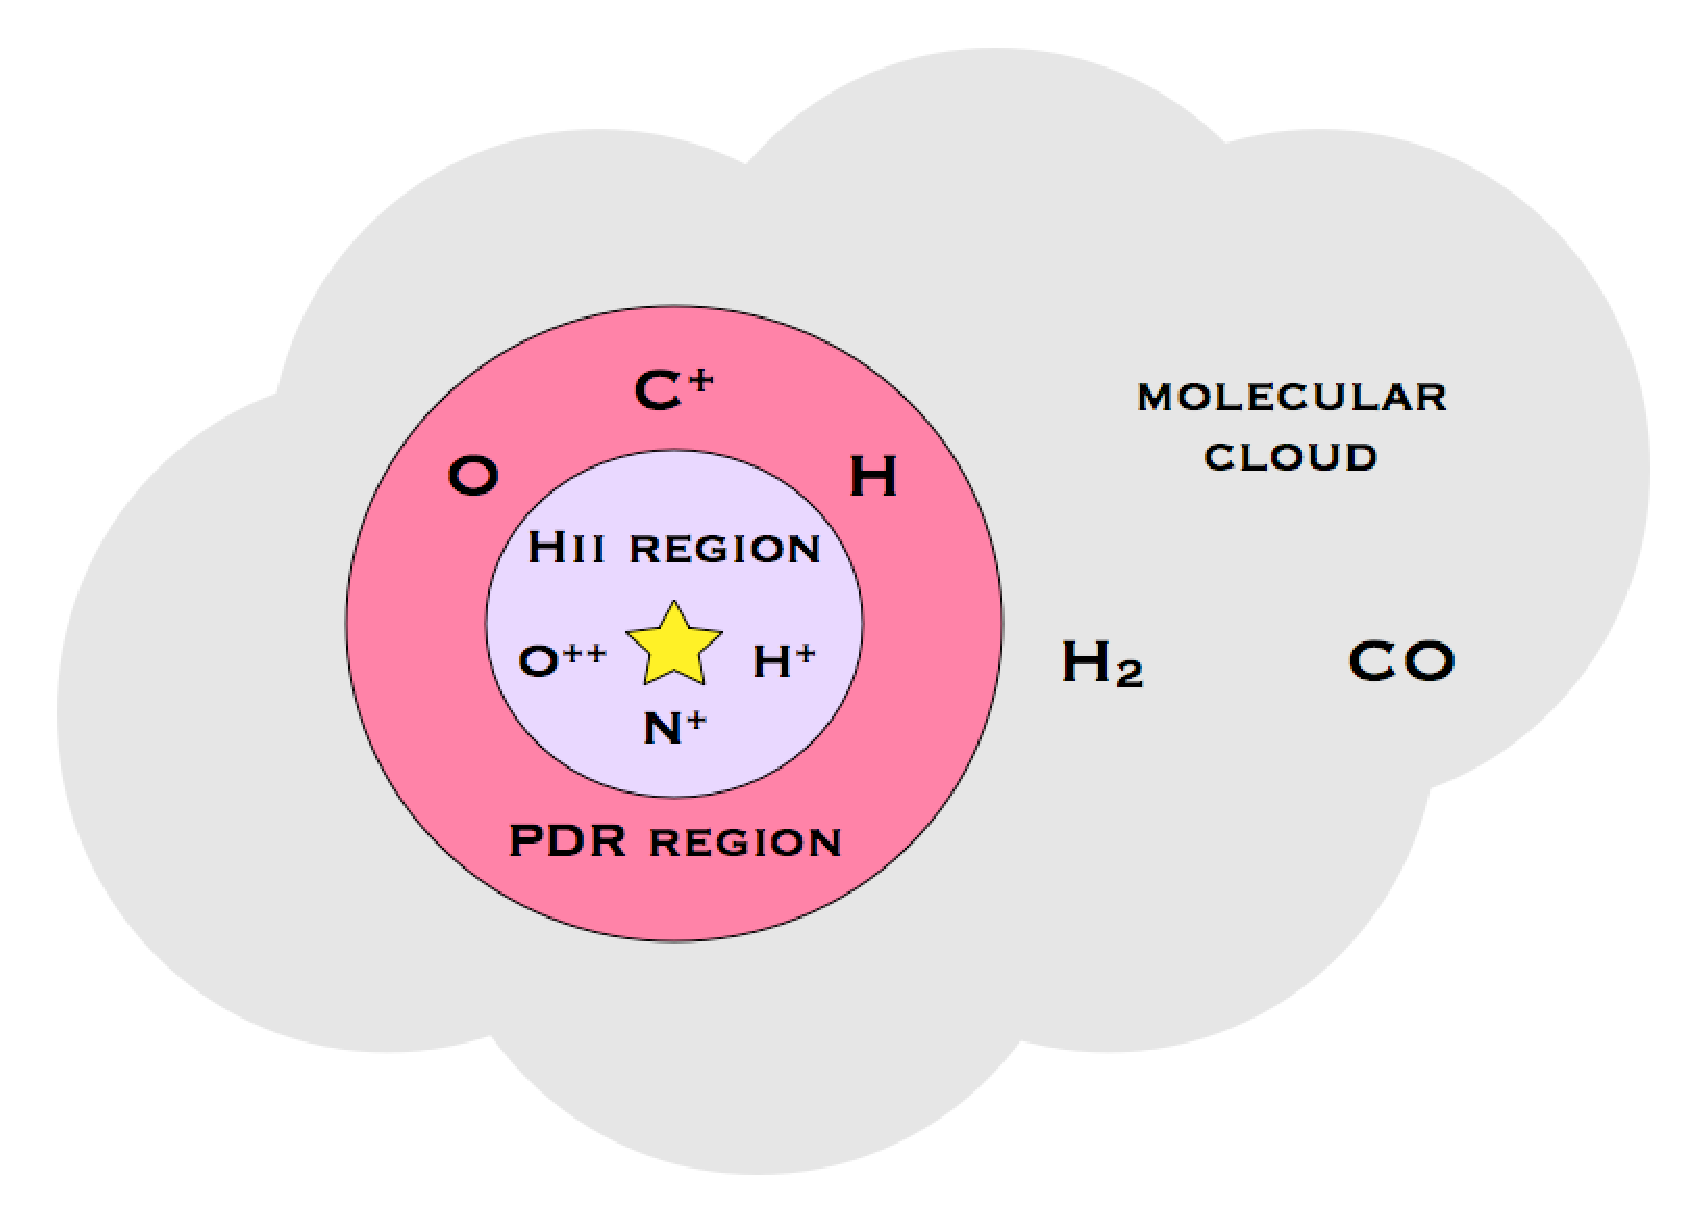
\includegraphics[width=\columnwidth]{ch1/molecular_cloud_schematic.eps}
  \caption[A cartoon of a molecular cloud]{A cartoon schematic of a molecular with an embedded stellar cluster and surrounding H~\textsc{ii} and PDR regions.
  \label{fig:cloud}}
 \end{center}
\end{figure}

\subsection{Important Gas Tracers} \label{gas_tracer}
Determining the physical conditions of the gas within the ISM involves observations of various atoms, ions and molecules and subsequent comparison of these observations with a theoretical model representing the ISM phase of interest.  Here we describe some of the most important gas tracers, how they are produced and how we observe them.

\subsubsection{Cold Gas}\label{cold_gas}
As stated above, the majority of a star forming galaxy's mass is found in neutral atomic and molecular hydrogen.  Atomic hydrogen is probed via the ``21~cm'' line using radio telescopes, and some of the earliest reports of observations of this line in our Milky Way are summarised by \citet{1951AJ.....56..144V}.  Studies of the H~\textsc{i} 21~cm line emission show that the atomic hydrogen distribution in galaxies is more extended than the optical disk \citep[e.g.][]{1997A&A...324..877B,2010ASPC..438....3T}.  The ubiquity of the atomic gas lends support to the importance of atomic hydrogen in understanding the properties of the ISM and the dynamics of a galaxy.  A morphological exception is early type galaxies (ellipticals and lenticulars), which often show few detections in atomic gas \citep[e.g.][]{1985AJ.....90..454K,1987IAUS..127..145K,1995A&A...300..675H,2010MNRAS.409..500O}.

Molecular gas is a more direct tracer of star formation than atomic gas, as star formation occurs in molecular clouds.  Observing molecular hydrogen (H$_{2}$) in its ground state is very difficult because it does not have an electric dipole moment \citep{1991ARA&A..29..581Y}.  Thus, we trace it indirectly using observations of the $J=1-0$ rotational transition of carbon monoxide (CO) and an empirically determined relation between the column density of H$_{2}$ and the integrated intensity of CO, the ``CO-to-H$_{2}$ conversion factor'', $X_{\mathrm{CO}}$ \citep[e.g.][]{1991ARA&A..29..581Y}.  The typical value of this conversion factor is $2 \times 10^{20}$~cm$^{-2}$~(K~km~s$^{-1}$)$^{-1}$ \citep{1988A&A...207....1S}, although this value is different in ultra luminous infrared galaxies \citep{1998ApJ...507..615D}, and can vary with radius and metallicity \citep[e.g. ][ and references therein]{2013arXiv1301.3498B}.  Higher level rotational transitions are useful tracers of warmer molecular gas \citep{2009ApJ...693.1736W}.  One way to observe molecular hydrogen directly is through its quadrupole moment rotational transitions, which produce spectral lines in the infrared \citep{1991ARA&A..29..581Y}, accessible through observatories such as \emph{Spitzer}.  It is also possible to observe H$_{2}$ directly via vibrational transitions of an electronically excited molecule, giving rise to spectral lines at around 2~$\mu$m \citep{2005pcim.book.....T}.  Lastly, one can observe H$_{2}$ absorption lines in the ultraviolet Lyman-Werner bands, which indicate upward electronic transitions \citep{2005pcim.book.....T}.

\subsubsection{H~\textsc{ii} regions and PDRs}\label{fine_lines}
Atomic fine structure lines are the most important spectral lines for tracing hot ionised gas in H~\textsc{ii} regions and the cool neutral gas in PDRs.  These lines contribute to the total cooling of the gas in their respective environments by removing thermal energy from the gas.  Gas heating occurs when radiation (usually FUV) from nearby stars provides photons which eject electrons from dust grains or polycyclic aromatic hydrocarbons (PAHs) via the photoelectric effect \citep{1985ApJ...291..722T,1991ApJ...377..192H}.  These free electrons subsequently contribute to the thermal energy of the gas.  Depending on the temperature of the gas, certain atoms and ions can be collisionally excited, and if the density of the gas is less than the critical density, which is the ratio of the spontaneous emission coefficient $A_{ij}$ divided by the collisional rate coefficient $\gamma_{ij}$, these excited atoms will most often emit a photon via a fine structure transition rather than collisionally de-excite, as shown in Figure~\ref{fig:cooling} \citep{2005pcim.book.....T}.

\begin{figure}[!h]
 \begin{center}
 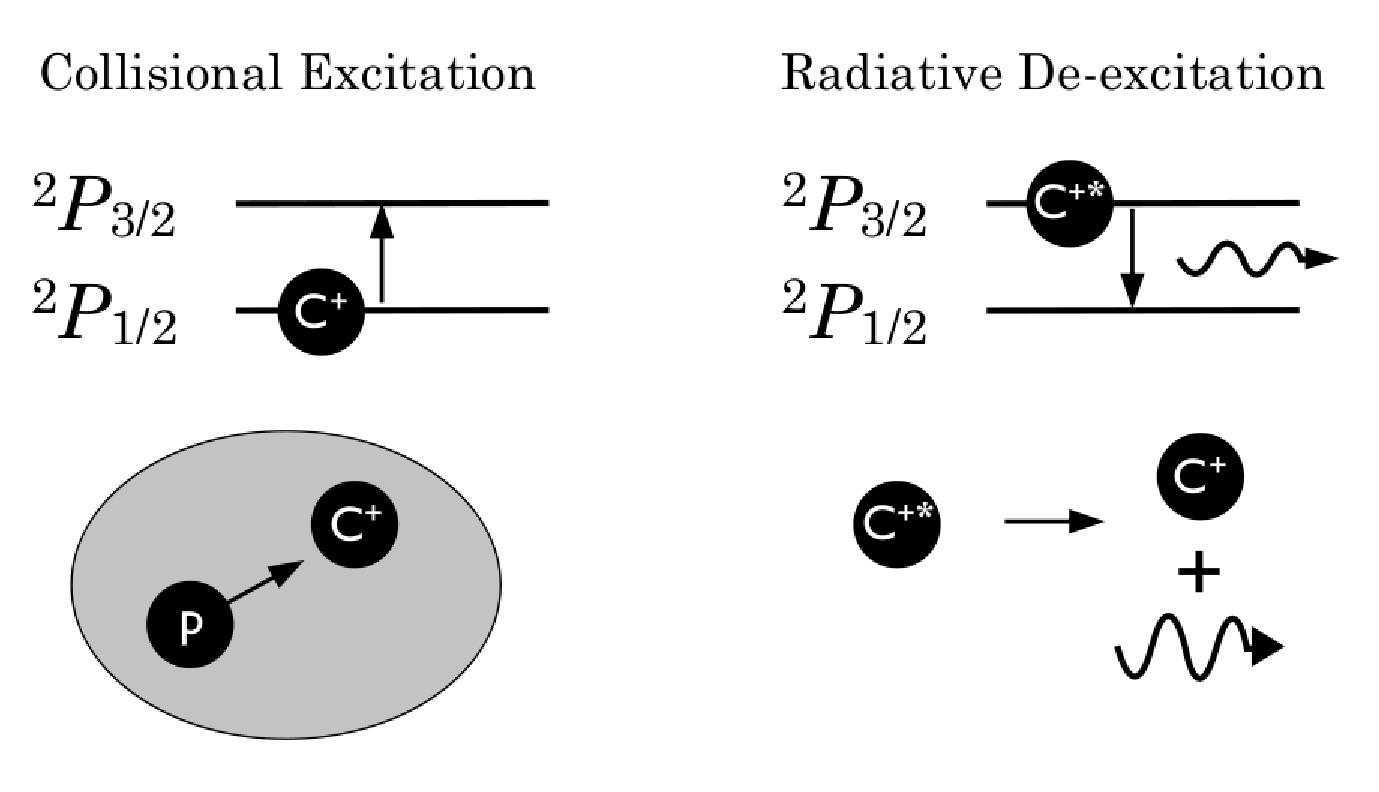
\includegraphics[width=\columnwidth]{ch1/cooling_line_schematic.eps}
  \caption[A cartoon of the cooling process via the \mbox{[C~\textsc{ii}](158~$\mu$m)} fine structure line]{A cartoon schematic of the collisional excitation and subsequent radiative de-excitation of a C$^{+}$ atom via the [C~\textsc{ii}](158~$\mu$m) transition.  The C$^{+}$ atom is collisionally excited by a collision with a particle such as a proton or electron and makes an upward transition from the $^{2}P_{1/2}$ state to the $^{2}P_{3/2}$ state.  The excited carbon ion, C$^{+*}$, then returns to the ground state by emitting a photon, thus removing thermal energy from the gas.
  \label{fig:cooling}}
 \end{center}
\end{figure}

In an H~\textsc{ii} region the radiation field is hard enough to ionise atoms or ions with ionisation potentials greater than 13.6~eV, such as N$^{+}$, N$^{++}$ and O$^{++}$.  Among the brightest mid- and far-infrared cooling lines in these regimes are the [N~\textsc{ii}] lines at 122 and 205~$\mu$m, the [O~\textsc{iii}] line at 88~$\mu$m, and the [N~\textsc{iii}] line at 57~$\mu$m, although there are many more cooling lines that contribute to the overall energy balance of the ionized gas \citep[e.g. ][]{2001ApJ...553..121H,2012A&A...548A..20C,2012A&A...548A..91L}.

In the neutral gas within PDRs the excited atoms have ionisation potentials less than 13.6~eV.  Here, species such as C, C$^{+}$, O and CO are the important coolants. The [C~\textsc{ii}] fine structure line at 158~$\mu$m dominates the cooling in this environment in most normal galaxies, contributing roughly 1~\% of the total cooling budget of a galaxy \citep{1985ApJ...291..755C,1991ApJ...373..423S,2001ApJ...561..766M}; however, it can be suppressed in ultraluminous infrared galaxies \citep[e.g. ][]{1998ApJ...504L..11L,2003ApJ...594..758L}.  Other important PDR diagnostics include the [O~\textsc{i}] lines at 63 and 145~$\mu$m, and the various CO rotational transitions \citep{2001ApJ...561..766M,2001A&A...375..566N}.

\subsection{Interstellar Dust} \label{dust}
Dust is ubiquitous throughout the ISM and its thermal emission produces about half of the infrared continuum radiation observed in galaxies \citep{2010A&A...518L...1P}.  It is an important component of the ISM and molecular clouds in particular, as it shields strong radiation emitted by hot stars from penetrating deep into the cloud.  Dust also acts as a catalyst for the formation of H$_2$, polycyclic aromatic hydrocarbons (PAHs), and other molecules \citep{2005pcim.book.....T}.

The exact composition of dust grains is still debated in the literature but in general there is agreement that they fall into two broad categories, carbons and silicates (or other heavier non-carbon based grains), although a mixture of the two has also been put forth by some models.  Another important component, though not strictly dust grains but rather large molecules, is polycyclic aromatic hydrocarbons.  These are large planar molecules comprising carbon atom chains arranged in a hexagonal pattern with hydrogen atoms bonded to the outermost atoms, and their vibrational modes produce spectral lines at mid-infrared wavelengths \citep{1985ApJ...290L..25A}.

One of the pioneering dust models was put forth by \citet{1977ApJ...217..425M} to model the observed interstellar extinction curve, who proposed that the grain population comprised a mix of naked graphite particles plus particles of a different material such as silicates or iron-based particles.  They found that the observations were best matched by a model with a range in size of the dust grains between 0.005~$\mu$m to 1~$\mu$m for the graphites and 0.025 to 0.25~$\mu$m for the other grains, following a power law distribution.  Several later models have either adopted the size distribution of \citet{1977ApJ...217..425M} or further investigated the composition of the dust using only the graphite and silicate type dust grains \citep[e.g. ][]{1984ApJ...285...89D, 1994ApJ...422..164K}.  \citet{2001ApJ...554..778L} expanded the graphite and silicate model by adding a PAH component, represented by extending the grains down in size to as small as a few Angstroms in diameter and attributing to the very small carbonaceous grains the properties of PAHs.  One of the most recent models from this class is by \citet{2007ApJ...657..810D}, which is now commonly used by observers (see below).

Other dust modellers have attempted to fit observations with alternative types of dust grains.  For example, some authors such as \citet{1989ApJ...341..808M} consider `fluffy' dust grains that are a combination of amorphous carbon, graphite and silicate particles loosely stuck together, as well as particles comprising just graphite. Later, \citet{1996ApJ...472..643M} proposed a dust model of purely graphite, purely silicate, and fluffy composite grains of a mix of carbon, silicates and other elements. \citet{2004ApJS..152..211Z} consider a dust model with different sets of dust grain compositions (such as that of \citet{2001ApJ...554..778L}, one testing the effects of including amorphous carbon instead of graphite, one including other heavier composite grains, and even one with only PAHs and no large carbon-based grains) to reproduce several observational constraints, and find that multiple models adequately fit the observations, emphasising the difficulty in establishing the exact nature of the dust grains.  Lastly, a third model has been suggested that consists of dust grains with a silicate centre surrounded by a carbon-based coating, in addition to PAHs and carbon dominated very small grains \citep[e.g.][]{1990A&A...237..215D}.

As the dust grain modelling implies, grain sizes span a large range from small grains approximately 5~$\mbox{\AA}$ in diameter up to very large grains of approximately 1~$\mu$m.  Large grains are in thermodynamic equilibrium with their environment and emit radiation in the far-infrared and submillimetre wavebands, corresponding to temperatures of roughly 20~K \citep{2003ARA&A..41..241D}.  Smaller dust grains tend to be out of equilibrium with their surroundings and are stochastically heated due to their small size.  A single photon can significantly increase the temperature of a small dust grain, which then slowly re-radiates away that energy, thus producing a significant fraction of the radiation at wavelengths shorter than about 50~$\mu$m \citep{2003ARA&A..41..241D}.

Modelling the observed spectral energy distribution of a galaxy or region within a galaxy can reveal properties of the dust grains such as composition, temperature and approximate size, depending on the type of model one uses.  The simplest approach is to fit a modified blackbody (graybody) function, described by
\begin{equation}\label{eqn:bb}
 I(\nu,T) = C\nu^{\beta}B(\nu,T),
\end{equation}
to observed photometry at far-infrared to submillimetre wavelengths.  Here, $B(\nu,T)$ is the Planck function, $\nu^{\beta}$ is from the empirical equation for the dust opacity, $\kappa_{\nu} = \kappa_{0}(\nu/\nu_{0})^{\beta}$, with $\beta$ the dust emissivity, and $C$ is a scaling constant encompassing the distance to the source, the dust mass, and the factor $\kappa_{0}/\nu_{0}^{\beta}$ from the dust opacity function.  From a theoretical perspective, $\kappa$ and $\beta$ are functions of the properties of the dust grains \citep[e.g.][]{1984ApJ...285...89D} and thus $\kappa_0$ may be calculated using a dust grain model for $\nu_0$ \citep{2001ApJ...554..778L}.  The factor $\beta$ is often left as a free parameter when fitting observations, but a value of $\beta=2.0$ is a common result \citep[e.g. ][]{1995ApJ...451..188R,2003AJ....125.2361B,2012A&A...540A..54B,2012MNRAS.421.2917F}.  Thus, $\beta$ can also be fixed at 2.0 when modelling observations.

The other common way to model the dust SED of a galaxy is to incorporate a more sophisticated dust model into the fitting.  The most commonly used of these models is that of \citet{2007ApJ...657..810D}, which updates some of the properties of the dust grain models of \citet{2001ApJ...554..778L} and \citet{2001ApJ...548..296W}.  This model considers dust grains comprised of silicates, carbonaceous grains, and PAHs and parameterises the radiation field the dust is exposed to by a parameter $U$, which is a dimensionless quantity such that $u_{\nu} = Uu_{\nu}^{\mathrm{MW}}$ is the energy density of the field and $u_{\nu}^{\mathrm{MW}}$ is the energy density in the Solar neighbourhood from \citet{1983A&A...128..212M}.  The bulk of the interstellar dust (represented by a fraction $(1-\gamma)$) is exposed to a radiation field with a scaling factor of $U_{\mathrm{min}}$, while dust in the vicinity of PDRs (represented by a fraction $\gamma$) is exposed to an effective radiation field represented by a power-law distribution of radiation fields with scaling factors between $U_{\mathrm{min}}$ and $U_{\mathrm{max}}$.  Fitting the model to observed photometry can produce a best-fitting model spectrum and return information on several free parameters, namely $U_{\mathrm{min}}$, $\gamma$ and the fractional abundance of PAHs, $q_{\mathrm{PAH}}$, which in turn can be used to calculate secondary information such as the total dust mass.

Another dust SED model in the literature is that of \citet{1990A&A...237..215D}.  It too considers silicate, carbonaceous and PAH grains, although in this model the silicate grains are coated or mixed with carbonaceous material, rather than being purely silicate as is the case for the \citet{2007ApJ...657..810D}.  This model has three components that are allowed to vary to best fit the observed spectrum, namely the PAH spectrum, the very small grain (carbon dominated grains) spectrum, and the big grain (silicate-carbon composite) spectrum.  However, it requires that the radiation field be first calculated then entered as an input parameter, rather than being integrated into the code itself.  This work became the basis for the model of \citet{2001ApJ...549..215D}, who first introduced the parameterisation of the radiation field with $U$, and more recently that of \citet{2011A&A...536A..88G}, although that particular model was designed to work with low-metallicity environments.

%%%%%%%%%%%%% Galaxies
%Furthermore, they are often found in groups \citep{1983ApJS...52...61G}, such as our own Local Group, and clusters of galaxies such as the Virgo Cluster.
\section{The Interstellar Medium of Galaxies}\label{galaxies}
Galaxies come in a wide variety of morphological shapes and sizes, presenting us with a wealth of environments to study.  Based on their optical appearances they are classified loosely as either spiral galaxies, elliptical and lenticular galaxies, and in some cases, irregular galaxies \citep{1926ApJ....64..321H}.  Here we discuss briefly the basic properties of galaxies in each of the two major categories and give some details for the individual galaxies M51 and Centaurus~A, which are the particular focus of this thesis.

\subsection{Spiral Galaxies}\label{spirals}
Spiral or disk galaxies each consist of a disk, a central bulge, and a halo \citep{1998gaas.book.....B}, and vary in total mass between $10^{9}$ and $10^{12}$~M$_{\odot}$ \citep{carrol_ostlie}.  The disk is rich in gas (atomic and molecular) and dust and can extend as large as 50~kpc in radius \citep{carrol_ostlie}. The disk typically shows a spiral structure with arms extending outward from the centre or central bar; these arms appear more luminous at numerous wavelengths than the interarm regions due to an increase in ISM density and star formation.  These arms can vary in prominence from the grand-design style consisting of two distinct, symmetric arms, to flocculent, patchy arms \citep[e.g.][]{1926ApJ....64..321H,1982MNRAS.201.1021E,1987ApJ...314....3E,1998gaas.book.....B}.  The disk also contains a young stellar population in contrast to the bulge, which contains an older stellar population \citep[e.g.][]{1944ApJ...100..147B}.  The bulge is a spheroidal shape extending above and below the plane and can vary in size relative to the disk, often characterized by the bulge-to-disk ratio.   At the very centre of the bulge in most spiral galaxies are supermassive black holes, and some of these power active galactic nuclei, which expel energy outward via jets, radiation or wind \citep{2012ARA&A..50..455F}.  Lastly, the halo is a low density spheroidal region in which the disk sits.  It contains a population of globular clusters, old stars and dark matter \citep{1987AJ.....93..816K,1998gaas.book.....B}.  However, it is worthwhile noting that most galaxies are dark matter dominated everywhere, not just in the halo.

A number of surveys over the past decade have extensively studied the properties of the ISM in extragalactic sources.  In spiral galaxies there is a broad range of characteristics.  Atomic and molecular gas masses can range anywhere from $1 \times 10^{7}$--$1.4 \times 10^{10}$~M$_{\odot}$ and $7 \times 10^{6}$--$6 \times 10^{9}$~M$_{\odot}$, respectively, in nearby galaxies \citep[e.g.][]{2008AJ....136.2563W,2009AJ....137.4670L}.  There is also a wide range in temperatures for the dust populations.  \citet{2012MNRAS.425..763G} investigated two dust components, a warm one and a cold one, and found a range of cold dust temperatures between 19 and 25.2~K, and a range of warm dust temperatures between 56 and 63~K.  The total dust mass in spiral type galaxies ranges from 10$^{6.39}$--10$^{8.57}$ as found by the \emph{Spitzer} Infrared Nearby Galaxy Survey \citep{2007ApJ...663..866D}, while the dust-to-gas mass ratio is on average about 0.007 (corresponding to a gas-to-dust ratio of roughly 140).  More recently, \citet{2012MNRAS.425..763G} report dust masses in spirals between $\sim 5 \times 10^{6}$ and $1.4 \times 10^{8}$~M$_{\odot}$ via fitting the dust spectral energy distribution with a modified blackbody.  Thus, spiral galaxies encompass a vast set of characteristics for their ISM properties.

\subsubsection{M51}\label{m51_general}
M51 (NGC~5194), also known as the Whirlpool Galaxy is an excellent example of a grand design, spiral galaxy and is located roughly 9.9~Mpc away \citep{2009AstL...35..599T}.  Its optical disk is approximately $11.2\arcmin \times 6.9\arcmin$ (32.3~kpc~$\times$~19.9~kpc) in size at the 25$^{th}$ magnitude surface brightness level, $D_{25}$ \citep{2003PASP..115..928K}, while its disk as observed in H~\textsc{i} extends $\sim 12.4\arcmin \times 10.0\arcmin$ (35.7~kpc~$\times$~28.8~kpc) with a total mass of $2.54 \times 10^{9}$~M$_{\odot}$ \citep{2008AJ....136.2563W}.  The molecular hydrogen, H$_{2}$, has a total mass of $2 \times 10^{9}$~M$_{\odot}$ covering roughly $9\arcmin \times 6\arcmin$ and well traces the H~\textsc{i} emission.  However, the ratio of atomic-to-neutral gas varies from 0.1 in the centre to 20 at the edges \citep{2007A&A...461..143S} indicating that the centre of the galaxy is molecular gas dominated but transitions to atomic gas dominated with increasing radius \citep{2007A&A...461..143S}.  Studies of H$\alpha$ and Pa$\alpha$ emission show over 1000 H~\textsc{ii} regions and a star formation rate of roughly 4~M$_{\odot}$~yr$^{-1}$ \citep{2001AJ....122.3017S}.  The galaxy also has a weak Seyfert~2 nucleus \citep{1997ApJS..112..315H}.

The dust content in M51 has been studied extensively at infrared wavelengths.  \citet{2005ApJ...633..871C} first presented the \emph{Spitzer} photometry from the \emph{Spitzer} Infrared Nearby Galaxy Survey \citep[SINGS; ][]{2003PASP..115..928K} at 3.6, 4.5, 5.8, 8.0, 24, 70 and 160~$\mu$m.  They find that the spiral arms are well defined at infrared wavelengths, tracing PAH emission and warm dust.  Combining the infrared data with ultraviolet and optical maps they determine that the 24~$\mu$m emission can be used as a local tracer of the star formation rate in M51 and determine a star formation rate surface density of 0.015~M$_{\odot}$~yr$^{-1}$~kpc$^{-2}$.  \citet{2007ApJ...671..333K} complemented this study by also making use of the \emph{Spitzer} infrared data to study the star formation rate law.  They find a strong linear correlation in log-log space between the star formation rate surface density and the total hydrogen gas mass surface density, with a slope ranging from 1.37--1.56, consistent with that of the Kennicutt-Schmidt law \citep[which has a slope of $1.4 \pm 0.15$; ][]{1998ApJ...498..541K}.  More recently, \citet{2012ApJ...755..165M} utilized previously obtained infrared observations with \emph{Herschel} photometry at 70, 160, 250, 350 and 500~$\mu$m to carry out a detailed study of the dust via spectral energy distribution modelling.  They found dust temperatures varying between 20 and 25~K, and a total dust mass of $1.2 \times 10^{8}$~M$_{\odot}$.  The average gas-to-dust mass ratio is $94 \pm 17$, close to the average Galactic value of roughly 160 \citep{2004ApJS..152..211Z}.  In the same study, it was determined that the most recent starburst episode in M51 was less than 500~Myr ago.  Merger interactions between galaxies often trigger star formation, as demonstrated by numerical simulations \citep[e.g.][]{1996ApJ...464..641M}, and in M51, observations of the stellar population reveal that blue supergiants are found along the tidal tail between M51 and its companion \citep{2009AstL...35..599T}, supporting this theory.

\subsection{Elliptical Galaxies}\label{ellip}
Unlike spiral galaxies, elliptical galaxies generally do not have an obvious disk and instead are spheroidal in shape with a wide range of masses, between 10$^{7}$ and 10$^{13}$~M$_{\odot}$ and sizes from 0.1~kpc to over 100~kpc across \citep{carrol_ostlie}.  Elliptical galaxies contain large amounts of dark matter with mass-to-light ratios of upwards of 100~L$_{\odot}$~M$^{-1}_{\odot}$ \citep{carrol_ostlie} and may contain many globuler cluster systems.  They also follow a characteristic surface brightness profile that falls off as radius$^{1/4}$ in optical bands \citep{1948AnAp...11..247D}, and generally contain smaller amounts of cold gas and dust than spiral galaxies \citep[e.g.][]{2004A&A...416...41X, 2010ApJ...725..100W,2011MNRAS.414..940Y,2012ApJ...748..123S}.

Once thought to contain very little ISM, we now know that a significant fraction of early type galaxies do, in fact, contain gas and dust.  The ATLAS$^{3\mathrm{D}}$ survey \citep{2011MNRAS.414..940Y}, consisting of a sample of 260 early type galaxies with a median stellar mass of $3 \times 10^{10}$~M$_{\odot}$, found a 20\% detection rate in CO emission, implying the presence of molecular gas.  Of those galaxies with molecular mass, the amount ranges between 10$^{7}$ and 10$^{9.3}$~M$_{\odot}$.  The \emph{Herschel} Reference Survey \citep{2010PASP..122..261B} determined that dust was present in 50\% of their sample using the 250~$\mu$m waveband as an indicator \citep{2012ApJ...748..123S}.  Typical dust temperatures in early type galaxies range between 16 and 32~K, while dust masses are approximately $10^{4.5}$--10$^{7}$~M$_{\odot}$ \citep{1998ApJ...499..670B,2012ApJ...748..123S}.

\subsubsection{Centaurus~A}\label{cena_general}
Centaurus~A is a giant elliptical galaxy with a prominent dust lane running through the centre of the galaxy, located 3.8~Mpc away \citep{2010PASA...27..457H}.  It has a triaxial morphology implying no preferred axis of rotation and is approximately 20$\arcmin$ (22.1~kpc) in diameter as seen in optical wavebands \citep{1998A&ARv...8..237I}.  The galaxy is also rich in globular clusters, with over 400 confirmed \citep{2007AJ....134..494W,2010ApJ...708.1335W}.  It is believed that the galaxy underwent a merger with a small spiral galaxy at some point during its past, resulting in the warped disk and peculiar overall appearance \citep{1944ApJ...100..147B,1993ApJ...412..550Q}.

The disk is rich in both atomic and molecular gas \citep[e.g.][]{1990ApJ...363..451E,1990AJ.....99.1781V,1992ApJ...391..121Q,2010A&A...515A..67S} with a total H~\textsc{i} mass of $\sim 4 \times 10^{8}$~M$_{\odot}$, and total H$_{2}$ mass of $\sim 4 \times 10^{8}$~M$_{\odot}$ \citep{2010PASA...27..463M}.  There have been shells detected in the outskirts of the galaxy (as far as 15$\arcmin$ (16.6~kpc) from the centre) in H~\textsc{i}, which strengthen the merger model \citep{1994ApJ...423L.101S}.  Infrared studies using \emph{Spitzer} IRAC observations by \citet{2006ApJ...645.1092Q} reveal a ring that resembles a parallelogram  as seen in the 3.6, 4.5, 5.8 and 8.0~$\mu$m wavebands.  It is modelled as a set of concentric rings at various inclinations giving rise to the warped disk morphology.

Cen~A also has a set of very large radio lobes powered by an active galactic nucleus.  The total area covered by the radio emission is roughly $8^{\circ} \times 4^{\circ}$ (530.6~kpc $\times$ 265.3~kpc) \citep{1997A&AS..121...11C}, though the prominent bubble shaped lobes extend roughly 5~kpc outward from the nucleus \citep{1998A&ARv...8..237I}.  The compact jets near the nucleus extend only about 1~pc from the centre \citep{1998A&ARv...8..237I}.  There is also a large amount of X-ray emission from Cen~A, spatially coincident with the nucleus, jets and lobes \citep[e.g.][]{1997ApJ...475..118T,2009ApJ...698.2036K}.

%%%%%%%%%%%%%% Herschel
\section{The Herschel Space Observatory} \label{herschel}
The first space observatory designed to observe the sky at mid- and far-infrared wavelengths was the \emph{Infrared Astronomical Satellite} (IRAS), which carried out an all-sky survey in 1983 at four wavelengths, 12, 25, 60 and 100~$\mu$m \citep{1984ApJ...278L...1N}.  This survey produced a number of catalogs containing upwards of $2.7 \times 10^{5}$ point sources and extended sources, as well as hundreds of spectra of select objects \citep{IRAS_supp}. Following the success of IRAS, the \emph{Infrared Space Observatory} (ISO), capable of both photometric and spectroscopic observations between 2.5 and 240~$\mu$m, was launched in 1995 \citep{1996A&A...315L..27K}.  ISO had numerous advantages over IRAS, including the ability for the observing community to propose for time on the telescope for their own projects.  During the same era as IRAS and ISO the \emph{Kuiper Airborne Observatory}, which started flying in 1975 \citep[e.g.][and references therein]{1979PASP...91..143H}, complemented the space-based observations by conducting regular flights observing the sky at high altitudes using a variety of instruments over its roughly 20 year lifetime.

Striving to produce increasingly higher resolution images of everything from embedded young stellar objects to high-redshift sources, the National Aeronautics and Space Administration (NASA) created the \emph{Spitzer Space Telescope} \citep[hereafter \emph{Spitzer}; ][]{2004ApJS..154....1W}, launched in 2003.  \emph{Spitzer} has a primary mirror with a diameter of 85~cm \citep{2004ApJS..154....1W}, and two photometers and a spectrometer on board.  The Infrared Array Camera (IRAC) conducted photometry at 3.6, 4.5, 5.8 and 8~$\mu$m \citep{2004ApJS..154...10F} and is still observing today at the two shortest wavelengths.  The Multiband Imaging Photometer for \emph{Spitzer} (MIPS) also conducted photometry, but at the mid- to far-infrared wavelengths 24, 70 and 160~$\mu$m \citep{2004ApJS..154...25R}, spanning the peak dust continuum emission.  Lastly, the Infrared Spectrograph (IRS) could obtain spectra between 5.3 and 38~$\mu$m \citep{2004ApJS..154...18H}.  \emph{Spitzer} ran out of the cryogen that kept the telescope at just a few degrees above absolute zero in 2009 \citep{2010SPIE.7731E..17C}, thus beginning the warm mission.  The end of \emph{Spitzer}'s cold mission paved the way for the next set of far-infrared observatories. In May of 2009, the \emph{Herschel Space Observatory} \citep[hereafter \emph{Herschel}; ][]{2010A&A...518L...1P} was launched by the European Space Agency (ESA) with some involvement by NASA, while the joint NASA and German Aerospace Center (DLR) flying \emph{Stratospheric Observatory for Infrared Astronomy} (SOFIA) was also inaugurated in 2010 \citep{2012ApJ...749L..17Y}.  The majority of data acquired for this thesis come from \emph{Herschel}, thus taking advantage of the best far-infrared data currently available for analysis.

The \emph{Herschel Space Observatory} has revolutionised our view of the Universe in the regime of the far-infrared and submillimetre astronomy.  The primary mirror is currently the largest in space at 3.5~m in diameter \citep{2010A&A...518L...1P}, and the observatory has three instruments capable of photometric and spectroscopic observations on board: the Photodetector Array Camera and Spectrometer \citep[PACS; ][]{2010A&A...518L...2P}, the Spectral and Photometric Imaging REceiver \citep[SPIRE; ][]{2010A&A...518L...3G}, and the Heterodyne Instrument for the Far Infrared \citep[HIFI; ][]{2010A&A...518L...6D}.  A summary of the major properties of each instrument in comparison to previous observatories is presented in Table~\ref{tbl:herschel_prop}.  PACS covers similar wavelength ranges to both \emph{Spitzer} and ISO, but at much higher angular resolution (see Table~\ref{tbl:herschel_prop}).  SPIRE's wavelength range covers longer wavelengths than have been observed before by a space observatory, and in some cases, for the first time ever.  Furthermore, the SPIRE Fourier Transform Spectrometer (FTS) has the major advantage of being able to obtain the complete spectrum of a target, rather than discrete parts of the spectrum centred on select spectral lines or wavelength ranges.  In contrast to both the PACS spectrometer and the SPIRE FTS, HIFI makes use of heterodyne receivers to collect continous spectra between 157 and 213~$\mu$m, and 240 and 625~$\mu$m using seven bands.  A selection of some of the most interesting scientific discoveries \emph{Herschel} has made, focusing on those most relevant to this thesis, are discussed below.

\begin{landscape}
\begin{deluxetable}{lccccc}
\tabletypesize{\small}
\tablecolumns{5}
\tablecaption{A comparison of \emph{Herschel} to previous space observatories \label{tbl:herschel_prop}}
\tablewidth{0pt}
\tablehead{
\colhead{Property} & \multicolumn{4}{c}{Observatory} \\
\colhead{} & \colhead{\emph{Herschel}\tablenotemark{a}} & \colhead{\emph{Spitzer}\tablenotemark{b}} & \colhead{ISO\tablenotemark{c}} & \colhead{IRAS\tablenotemark{d}} 
}
 \startdata
 Primary Mirror diameter (m) & 3.5 & 0.85 & 0.6 & 0.6 \\
 Photometric Wavebands   & 70, 100, 160 (PACS) & 3.6, 4.5, 5.8, 8 (IRAC) & 2.5--5.5, 4--18 (ISOCAM) & 12, 25, 60, 100 \\
 ($\mu$m)                & 250, 350, 500 (SPIRE) & 24, 70, 160 (MIPS) & 3--120, 50--240 (ISOPHOT) &  \\
 Spectroscopic Wavelength & 55--210 (PACS)   &  5.3--38 (IRS) & 2.4--45.2 (SWS) & 8--13, 11--23 \\
 ($\mu$m)                 & 157--625 (HIFI)  &                & 43--197 (LWS) &  \\
                          & 194--671 (SPIRE) &  &  &  \\
 Photometric FWHM ($\arcsec$) & & & \\
  of select wavelengths: & & & \\
 \quad $\sim$24--25~$\mu$m    &        --       & 6  & 23 & 240--360 \\
 \quad 60 or 70~$\mu$m   &   $5.5 \times 5.8$   & 18 & 50--60 & 240--360 \\
 \quad 100~$\mu$m        &   $6.7 \times 6.9$   & -- & $\sim 80$ & 240-360 \\
 \quad 160~$\mu$m\phm{ISOCAMgapgap} &   \phm{gap}$10.5 \times 12.0$\phm{gap} & \phm{gapgapgap}40\phm{gapgapgap} & \phm{gapgapgap}134\phm{gapgapgap} & \phm{gapgap}--\phm{gapgap}\\
 \enddata
 \tablenotetext{a}{PACS: \citet{2010A&A...518L...2P}, SPIRE: \citet{2010A&A...518L...2P}, HIFI: \citet{2010A&A...518L...6D}; PACS FWHM from the \citet{pacs_om}, SPIRE FWHM from the \citet{spire_om}}
 \tablenotetext{b}{IRAC: \citet{2004ApJS..154...10F}, MIPS: \citet{2004ApJS..154...25R}, IRS: \citet{2004ApJS..154...18H}}
 \tablenotetext{c}{ISOCAM: \citet{1996A&A...315L..32C}, SWS: \citet{1996A&A...315L..49D}, LWS: \citet{1996A&A...315L..38C}; FWHM values from The ISO Handbook \citep{ISO_handbook}.}
 \tablenotetext{d}{IRAS Explanatory Supplement \citep{IRAS_supp}}
\end{deluxetable}
\end{landscape}


\subsection{Herschel Science Highlights} \label{herschel_sci}
There were many goals across various categories within astronomy set for \emph{Herschel} before it was launched, and it has certainly met and arguably exceeded a number of them already.  The mission has just come to an end, but many more results are still to come as the data become fully exploited by the astronomy community.  Advances and discoveries have been made in a number of areas from young embedded stellar objects to the distant Universe.  For example, \citet{2012A&A...540A.125A} presented \emph{Herschel} observations of a debris disk around the star Fomalhaut that indicate that the star's disk is active in producing fluffy dust grains via collisions, giving us insight into the dynamics of exoplanetary systems.  On slightly larger scales, \emph{Herschel} observations are revealing more clues about star formation.  Initial analysis of two subregions of the Herschel Infrared GALactic plane survey \citep[Hi-Gal; ][]{2010PASP..122..314M, 2010A&A...518L.100M} by \citet{2010A&A...518L..97E} found a total of almost 1000 embedded cores, and SED modelling of a subset of these objects indicates a large fraction of them are forming high-mass stars despite possessing lower than critical core gas mass surface densities.  This critical threshold is a theoretical value for the surface density of the gas that cores must surpass in order to form massive stars, and is derived to be 1~g~cm$^{-2}$ \citep{2008Natur.451.1082K}.  \emph{Herschel}'s high resolution photometry has also revealed that molecular clouds are filled with a cobweb-like structure of filaments, which possess a characteristic width of 0.1~pc that likely stems from the dissipation of turbulence \citep{2011A&A...529L...6A}.  These filamentary structures also appear to be the primary hosts of star-forming regions within a molecular cloud.

\emph{Herschel} has also produced some spectacular observations of many well-known galaxies.  The HERschel Inventory of The Agents of Galaxy Evolution \citep[HERITAGE; ][]{2010A&A...518L..71M} team is investigating the Small and Large Magellanic Clouds (SMC and LMC, respectively) in search of understanding the evolution of the ISM in a low-metallicity environment, one that might mimic primordial galaxies at high redshift.  \citet{2010A&A...518L..71M} presented early science results for the LMC and determined that the dust grains are likely composed of amorphous carbon and silicates rather than graphite and silicates.  One interesting result that stemmed from the \emph{Herschel} photometry of the LMC is the first far-infrared and submillimetre detection of Supernova~1987A.  An investigation of this emission showed that the dust coincident with the location of the remnant has been produced by the supernova ejecta, indicating quick processing of material post-event \citep{2011Sci...333.1258M}.  A study of the ultra-luminous infrared galaxy (ULIRG) Arp~220 by \citet{2011ApJ...743...94R} using the SPIRE Fourier Transform Spectrometer (FTS) revealed that this extreme environment hosts an X-ray luminous active galactic nucleus (AGN) at its centre and a wealth of molecules in various energy states in its gas component.  Furthermore, the mechanical energy of the merger in this galaxy is affecting this molecular gas.  The \emph{Herschel} Virgo Cluster Survey has presented numerous results thus far, one of which focuses on the dust-to-gas ratio of the spatially resolved members of the Virgo Cluster \citep{2012A&A...545A..75P}.  These authors find among other things a radially increasing or flat trend in the dust-to-gas ratio with increasing radius for galaxies deficient in atomic gas, and they conclude that the cluster environment is having an effect on the molecular gas and dust distributions within individual galaxy members.  The observations of the \emph{Herschel} Multi-tiered Extragalactic Survey have even revealed gravitationally lensed submillimetre galaxies, some of which would normally have fluxes too weak to be detected by SPIRE at 500~$\mu$m \citep{2013ApJ...762...59W}.

These are just a few of the many important and inspiring results published to date and there will be many more to come.  In this thesis, we focus on a unique set of observations from the PACS and SPIRE instruments, adding to the rich and diverse science produced with \emph{Herschel}.



%%%%%%%%%%%%%%%% PACS processing
\section{PACS Spectroscopy and Processing} \label{pac_spec}
A large portion of this thesis is spent analysing spectroscopy from the \emph{Herschel} PACS instrument; thus, it is useful to describe the data processing steps in more detail here than it appears in Chapters~\ref{chapter3} and \ref{chapter4}.  We refrain from detailing the PACS and SPIRE photometry reduction process further, as it is a more simple process and it is described sufficiently in Chapter~\ref{chapter2}.

The PACS spectrometer consists of 25 spatial pixels (spaxels) arranged in a $5 \times 5$ grid, with each spaxel covering a field of view on the sky of $9.4 \arcsec \times 9.4 \arcsec$ \citep{pacs_om}.  The spectral dimension in each spaxel is subdivided into 16 pixels, producing a spectral resolution of between approximately 75 and 300~km~s$^{-1}$ \citep{pacs_om}.  All of our PACS spectroscopic observations were carried out using the Line Spectroscopy mode, meaning we centred each observation on the spectral line we intended to target and the total wavelength range seen by the instrument was narrow, ranging from $\sim 0.35$--1.8~$\mu$m.  This wavelength range is stepped through by the instrument's grating during an observation such that each spaxel contains many individual spectra covering slightly different overlapping wavelength ranges, with the centre of the line being sampled by the most steps.  An example of these overlapping spectra for our [C~\textsc{ii}](158~$\mu$m) observations of the centre of M51 is shown in Figure~\ref{fig:data_cloud}.

\begin{figure}[!h]
 \begin{center}
 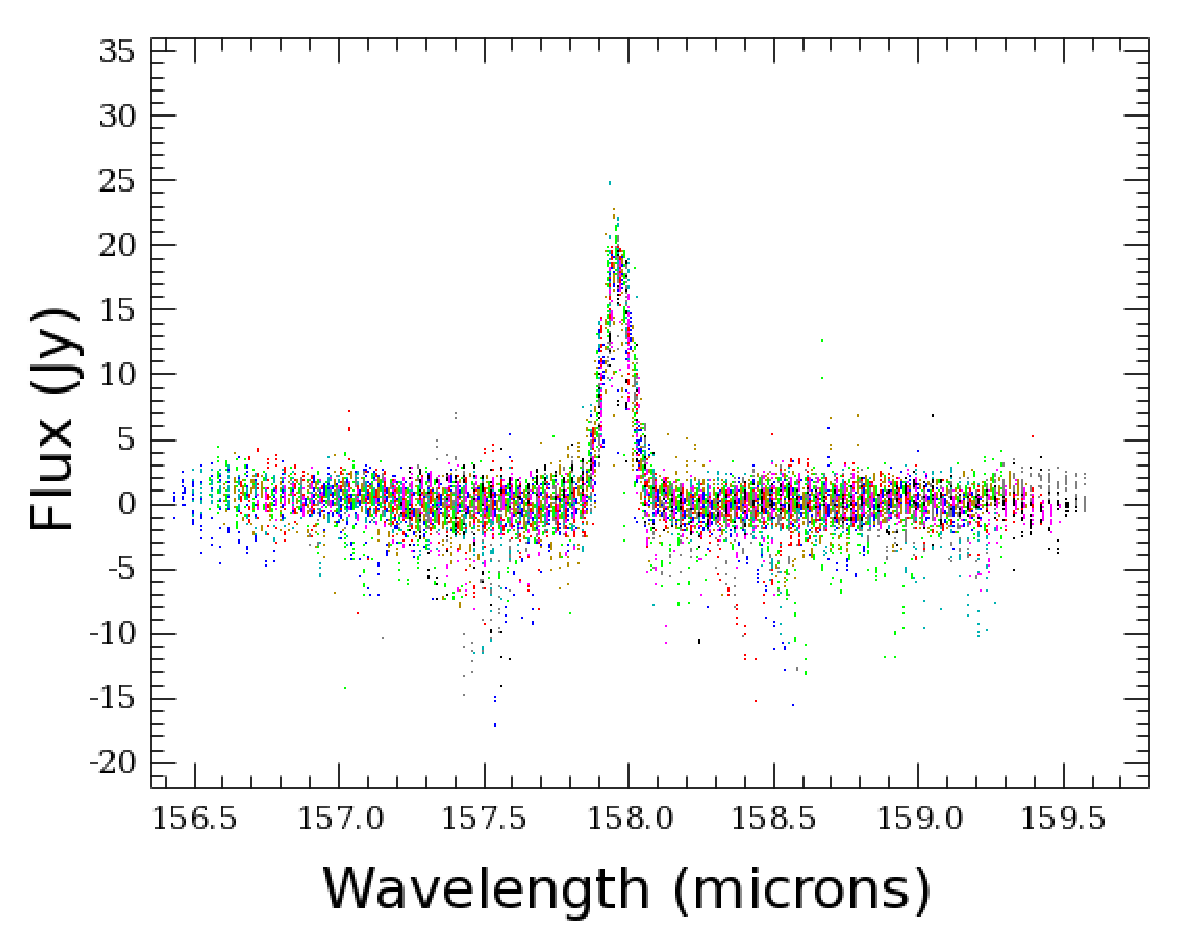
\includegraphics[width=\columnwidth]{ch1/M51_line_CII157.eps}
  \caption[Raw data cloud of a PACS \mbox{[C~\textsc{ii}](158~$\mu$m)} observation for M51]{An example of a PACS spectroscopic observation in its raw data form.  Shown is the spectrum of the [C~\textsc{ii}](158~$\mu$m) line in the central spaxel of one of the rasters of M51.
  \label{fig:data_cloud}}
 \end{center}
\end{figure}

The spectroscopic observations from the \emph{Herschel} PACS are initially processed using the Herschel Interactive Processing Environment \citep[HIPE; ][]{2010ASPC..434..139O} and Flexible Image Transport System (FITS) files holding the final spectral data are produced.  The line fitting and map making are done in a program called PACSman \citep{2012A&A...548A..91L}, which is an Interactive Data Language (IDL) package.

The line fitting iterates through each of the 25 spaxels comprising a single raster, and then through each raster if there is more than one, as is the case for both M51 (see Chapter~\ref{chapter3}) and Centaurus~A (see Chapter~\ref{chapter4}).  The fitting is carried out on the raw data produced in HIPE, prior to any rebinning, so as to obtain the best fit possible.  The continuum is fit first using a polynomial of up to a maximum of five orders, at the choice of the user.  For our observations, a second order polynomial was sufficient for the baseline fitting.  Next, the line is fit using a Gaussian function with the option of adding a broadening component for broader lines.  The parameters of the best fitting function, as well as the integrated flux, velocity information, full-width at half-maximum (FWHM) of the line, and continuum information are saved for the last step, map making.  An example of a [C~\textsc{ii}](158~$\mu$m) spectrum for M51 and its best fit are shown in Figure~\ref{fig:spectrum}.

\begin{figure}[!h]
 \begin{center}
 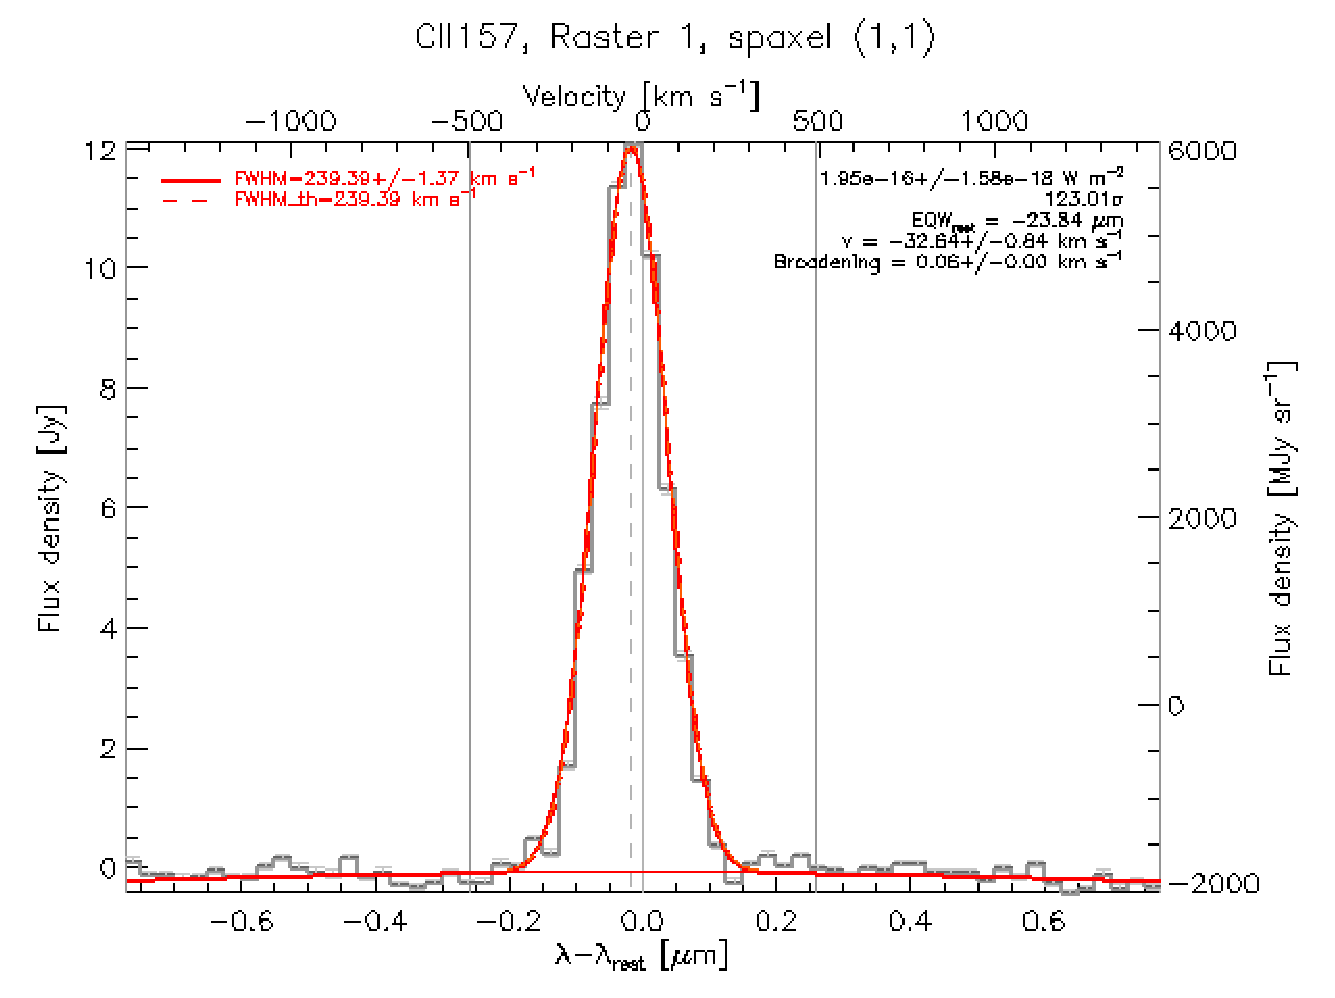
\includegraphics[width=\columnwidth]{ch1/M51_raster1_11.eps}
  \caption[Best line fit to a spaxel from PACS \mbox{[C~\textsc{ii}](158~$\mu$m)} observations of M51]{An example of a line fit to a [C~\textsc{ii}](158~$\mu$m) spectrum of M51 using PACSman.  The rebinned spectrum is shown in gray, the thin red line shows the best fit to the continuum, and the thick red line shows the best fit to the line.  The vertical gray lines mark the predicted line centre, and the two boundaries of the line component.  The vertical dashed line marks the observed line centre.
  \label{fig:spectrum}}
 \end{center}
\end{figure}

The maps are constructed by first laying down a grid with a pixel scale of $9.4 \arcsec /3$, corresponding to one-third of the original pixel scale of a raster (i.e. each pixel is subdivided into nine pixels at the new scale).  For each pixel in the final grid, the code iterates through all rasters searching for all contributing pixels.  Each contributing pixel is rotated through the appropriate position angle to align it to the final grid.  Next, the area of each original pixel that coincides with the selected final pixel is calculated as the weight for that pixel.  Finally, the weighted mean of the values of the contributing pixels is calculated and stored in the new pixel.  This process is completed for the flux, velocity, FWHM and continuum data and the new maps are stored as fits files for full analysis, along with their associated error maps.

%%%%%%%%%%%%%%%%%%% thesis outline
\section{This Thesis}\label{thesis_outline}
As described above, the infrared and submillimetre wavelength regime is important for probing the cold ISM.  With the unprecedented resolution of \emph{Herschel} we can now investigate the evolution of the cold regions of the ISM and the impact of star formation on not only molecular clouds in our own Milky Way, but in nearby galaxies as well.  Resolving details on scales of a few hundred parsecs in other galaxies gives us additional insight into the characteristics of the ISM and we can search for variations in these important properties within a single galaxy.  Extragalactic studies also allow us to look at each galaxy as a whole to broaden our undestanding, something that can be difficult to exploit in our own Galaxy, depending on the wavelength regime being used.  Thus, we can also compare and contrast ISM properties between galaxies of different morphologies to see how environment impacts the local ISM.

The \emph{Herschel} Very Nearby Galaxies Survey (VNGS; P.I. Christine Wilson) is a diverse sample of 13 galaxies located closer than roughly 80~Mpc away.  Centaurus~A (Cen~A; NGC~5128) and M51 (NGC~5194) are both sources that are a part of this survey.  M51 is classified as a grand-design, late-type spiral, SAbc \citep{1991trcb.book.....D}, and is oriented almost face-on to our line of sight.  Cen~A is classified as a peculiar S0 giant elliptical galaxy \citep{1991trcb.book.....D} and contains an embedded, edge-on disk.  Thus, at first glance they are quite different in morphology; however, both have active nuclei (CenA is a proper AGN and M51 is a low luminosity AGN) and have been affected by merger events.  Investigating the ISM in each galaxy affords us the ability to both search for regional variations as well as global morphological influence on the ISM.  In particular, we can compare and contrast the molecular cloud properties of the two galaxies and evaluate the possible influence of an active nucleus, a merger event, or spiral arms on the evolution and properties of the ISM.

In this thesis, we utilise observational data obtained from the James Clerk Maxwell Telescope and the \emph{Herschel} Space Observatory to investigate the gas and dust components of the ISM in Cen~A and M51.  Both observatories target wavelengths in the far-infrared and submillimetre regimes, key wavebands to study to enrich our understanding of the ISM.  Photometry from \emph{Herschel} allows us to model the observed spectral energy distribution (SED) on smaller scales, as well as at longer wavelengths than other space observatories.  \emph{Herschel}'s spectroscopic instruments have improved sensitivity and resolution over observatories such as ISO, allowing us to detect weaker far-infrared cooling lines that may have been previously undetected, in addition to better observations of the strongest lines.  Furthermore, the JCMT's HARP-B instrument allows us to probe the CO($J=3-2$) transition, adding additional information about the gas to our investigation.  Thus, we will study these two objects with the best data available to satisfy our scientific goals of contributing to the understanding of the evolution of the ISM.

This thesis is organised in the following manner.  In Chapter~\ref{chapter2} we present an investigation of the gas-to-dust ratio in Cen~A using \emph{Herschel} PACS and SPIRE photometry, as well as spectroscopy from the JCMT.  In Chapter~\ref{chapter3} we present an investigation of the molecular cloud properties of the inner region of M51 using photodissociation (photon dominated) region modelling of PACS spectroscopy, and in Chapter~\ref{chapter4} we carry out photodissociation region modelling on a radial strip of the disk of Cen~A.  We summarise the achievements of this work and discuss future directions in Chapter~\ref{chapter5}.

%\chapterbib
%\bibliography{thesis_bib}
%\bibliographystyle{apj}

\begin{thebibliography}{133}
\expandafter\ifx\csname natexlab\endcsname\relax\def\natexlab#1{#1}\fi

\bibitem[{{Acke} {et~al.}(2012){Acke}, {Min}, {Dominik}, {Vandenbussche},
  {Sibthorpe}, {Waelkens}, {Olofsson}, {Degroote}, {Smolders}, {Pantin},
  {Barlow}, {Blommaert}, {Brandeker}, {De Meester}, {Dent}, {Exter}, {Di
  Francesco}, {Fridlund}, {Gear}, {Glauser}, {Greaves}, {Harvey}, {Henning},
  {Hogerheijde}, {Holland}, {Huygen}, {Ivison}, {Jean}, {Liseau}, {Naylor},
  {Pilbratt}, {Polehampton}, {Regibo}, {Royer}, {Sicilia-Aguilar}, \&
  {Swinyard}}]{2012A&A...540A.125A}
{Acke}, B., {Min}, M., {Dominik}, C., {et~al.} 2012, \aap, 540, A125

\bibitem[{{Allamandola} {et~al.}(1985){Allamandola}, {Tielens}, \&
  {Barker}}]{1985ApJ...290L..25A}
{Allamandola}, L.~J., {Tielens}, A.~G.~G.~M., \& {Barker}, J.~R. 1985, \apjl,
  290, L25

\bibitem[{{Arzoumanian} {et~al.}(2011){Arzoumanian}, {Andr{\'e}}, {Didelon},
  {K{\"o}nyves}, {Schneider}, {Men'shchikov}, {Sousbie}, {Zavagno}, {Bontemps},
  {di Francesco}, {Griffin}, {Hennemann}, {Hill}, {Kirk}, {Martin}, {Minier},
  {Molinari}, {Motte}, {Peretto}, {Pezzuto}, {Spinoglio}, {Ward-Thompson},
  {White}, \& {Wilson}}]{2011A&A...529L...6A}
{Arzoumanian}, D., {Andr{\'e}}, P., {Didelon}, P., {et~al.} 2011, \aap, 529, L6

\bibitem[{{Baade}(1944)}]{1944ApJ...100..147B}
{Baade}, W. 1944, \apj, 100, 147

\bibitem[{{Bendo} {et~al.}(2003){Bendo}, {Joseph}, {Wells}, {Gallais}, {Haas},
  {Heras}, {Klaas}, {Laureijs}, {Leech}, {Lemke}, {Metcalfe}, {Rowan-Robinson},
  {Schulz}, \& {Telesco}}]{2003AJ....125.2361B}
{Bendo}, G.~J., {Joseph}, R.~D., {Wells}, M., {et~al.} 2003, \aj, 125, 2361

\bibitem[{{Bergin} \& {Tafalla}(2007)}]{2007ARA&A..45..339B}
{Bergin}, E.~A., \& {Tafalla}, M. 2007, \araa, 45, 339

\bibitem[{{Binney} \& {Merrifield}(1998)}]{1998gaas.book.....B}
{Binney}, J., \& {Merrifield}, M. 1998, {Galactic Astronomy}, Princeton Series
  in Astrophysics (Princeton, NJ: Princeton University Press)

\bibitem[{{Bolatto} {et~al.}(2013){Bolatto}, {Wolfire}, \&
  {Leroy}}]{2013arXiv1301.3498B}
{Bolatto}, A.~D., {Wolfire}, M., \& {Leroy}, A.~K. 2013, ArXiv e-prints

\bibitem[{{Boselli} {et~al.}(2002){Boselli}, {Lequeux}, \&
  {Gavazzi}}]{2002A&A...384...33B}
{Boselli}, A., {Lequeux}, J., \& {Gavazzi}, G. 2002, \aap, 384, 33

\bibitem[{{Boselli} {et~al.}(2010){Boselli}, {Eales}, {Cortese}, {Bendo},
  {Chanial}, {Buat}, {Davies}, {Auld}, {Rigby}, {Baes}, {Barlow}, {Bock},
  {Bradford}, {Castro-Rodriguez}, {Charlot}, {Clements}, {Cormier}, {Dwek},
  {Elbaz}, {Galametz}, {Galliano}, {Gear}, {Glenn}, {Gomez}, {Griffin}, {Hony},
  {Isaak}, {Levenson}, {Lu}, {Madden}, {O'Halloran}, {Okamura}, {Oliver},
  {Page}, {Panuzzo}, {Papageorgiou}, {Parkin}, {Perez-Fournon}, {Pohlen},
  {Rangwala}, {Roussel}, {Rykala}, {Sacchi}, {Sauvage}, {Schulz}, {Schirm},
  {Smith}, {Spinoglio}, {Stevens}, {Symeonidis}, {Vaccari}, {Vigroux},
  {Wilson}, {Wozniak}, {Wright}, \& {Zeilinger}}]{2010PASP..122..261B}
{Boselli}, A., {Eales}, S., {Cortese}, L., {et~al.} 2010, \pasp, 122, 261

\bibitem[{{Boselli} {et~al.}(2012){Boselli}, {Ciesla}, {Cortese}, {Buat},
  {Boquien}, {Bendo}, {Boissier}, {Eales}, {Gavazzi}, {Hughes}, {Pohlen},
  {Smith}, {Baes}, {Bianchi}, {Clements}, {Cooray}, {Davies}, {Gear}, {Madden},
  {Magrini}, {Panuzzo}, {Remy}, {Spinoglio}, \&
  {Zibetti}}]{2012A&A...540A..54B}
{Boselli}, A., {Ciesla}, L., {Cortese}, L., {et~al.} 2012, \aap, 540, A54

\bibitem[{{Bregman} {et~al.}(1998){Bregman}, {Snider}, {Grego}, \&
  {Cox}}]{1998ApJ...499..670B}
{Bregman}, J.~N., {Snider}, B.~A., {Grego}, L., \& {Cox}, C.~V. 1998, \apj,
  499, 670

\bibitem[{{Broeils} \& {Rhee}(1997)}]{1997A&A...324..877B}
{Broeils}, A.~H., \& {Rhee}, M.-H. 1997, \aap, 324, 877

\bibitem[{{Calzetti} {et~al.}(2005){Calzetti}, {Kennicutt}, {Bianchi},
  {Thilker}, {Dale}, {Engelbracht}, {Leitherer}, {Meyer}, {Sosey}, {Mutchler},
  {Regan}, {Thornley}, {Armus}, {Bendo}, {Boissier}, {Boselli}, {Draine},
  {Gordon}, {Helou}, {Hollenbach}, {Kewley}, {Madore}, {Martin}, {Murphy},
  {Rieke}, {Rieke}, {Roussel}, {Sheth}, {Smith}, {Walter}, {White}, {Yi},
  {Scoville}, {Polletta}, \& {Lindler}}]{2005ApJ...633..871C}
{Calzetti}, D., {Kennicutt}, Jr., R.~C., {Bianchi}, L., {et~al.} 2005, \apj,
  633, 871

\bibitem[{{Carey} {et~al.}(2010){Carey}, {Surace}, {Glaccum}, {Ingalls},
  {Krick}, {Lacy}, {Lowrance}, {Laine}, {O'Linger}, {Stauffer}, {Willner},
  {Hora}, {Hoffmann}, {Ashby}, {Huang}, {Marengo}, {Pahre}, {Wang}, {Werner},
  \& {Fazio}}]{2010SPIE.7731E..17C}
{Carey}, S.~J., {Surace}, J.~A., {Glaccum}, W.~J., {et~al.} 2010, in Society of
  Photo-Optical Instrumentation Engineers (SPIE) Conference Series, Vol. 7731,
  Society of Photo-Optical Instrumentation Engineers (SPIE) Conference Series

\bibitem[{{Carroll} \& {Ostlie}(2006)}]{carrol_ostlie}
{Carroll}, B.~W., \& {Ostlie}, D.~A. 2006, {An Introduction to Modern
  Astrophysics}, 2nd edn. (Addison-Wesley)

\bibitem[{{Cesarsky} {et~al.}(1996){Cesarsky}, {Abergel}, {Agnese}, {Altieri},
  {Augueres}, {Aussel}, {Biviano}, {Blommaert}, {Bonnal}, {Bortoletto},
  {Boulade}, {Boulanger}, {Cazes}, {Cesarsky}, {Chedin}, {Claret}, {Combes},
  {Cretolle}, {Davies}, {Desert}, {Elbaz}, {Engelmann}, {Epstein},
  {Franceschini}, {Gallais}, {Gastaud}, {Gorisse}, {Guest}, {Hawarden},
  {Imbault}, {Kleczewski}, {Lacombe}, {Landriu}, {Lapegue}, {Lena}, {Longair},
  {Mandolesi}, {Metcalfe}, {Mosquet}, {Nordh}, {Okumura}, {Ott}, {Perault},
  {Perrier}, {Persi}, {Puget}, {Purkins}, {Rio}, {Robert}, {Rouan}, {Roy},
  {Saint-Pe}, {Sam Lone}, {Sargent}, {Sauvage}, {Sibille}, {Siebenmorgen},
  {Sirou}, {Soufflot}, {Starck}, {Tiphene}, {Tran}, {Ventura}, {Vigroux},
  {Vivares}, \& {Wade}}]{1996A&A...315L..32C}
{Cesarsky}, C.~J., {Abergel}, A., {Agnese}, P., {et~al.} 1996, \aap, 315, L32

\bibitem[{{Clegg} {et~al.}(1996){Clegg}, {Ade}, {Armand}, {Baluteau}, {Barlow},
  {Buckley}, {Berges}, {Burgdorf}, {Caux}, {Ceccarelli}, {Cerulli}, {Church},
  {Cotin}, {Cox}, {Cruvellier}, {Culhane}, {Davis}, {di Giorgio}, {Diplock},
  {Drummond}, {Emery}, {Ewart}, {Fischer}, {Furniss}, {Glencross},
  {Greenhouse}, {Griffin}, {Gry}, {Harwood}, {Hazell}, {Joubert}, {King},
  {Lim}, {Liseau}, {Long}, {Lorenzetti}, {Molinari}, {Murray}, {Naylor},
  {Nisini}, {Norman}, {Omont}, {Orfei}, {Patrick}, {Pequignot}, {Pouliquen},
  {Price}, {Nguyen-Q-Rieu}, {Rogers}, {Robinson}, {Saisse}, {Saraceno},
  {Serra}, {Sidher}, {Smith}, {Smith}, {Spinoglio}, {Swinyard}, {Texier},
  {Towlson}, {Trams}, {Unger}, \& {White}}]{1996A&A...315L..38C}
{Clegg}, P.~E., {Ade}, P.~A.~R., {Armand}, C., {et~al.} 1996, \aap, 315, L38

\bibitem[{{Combi} \& {Romero}(1997)}]{1997A&AS..121...11C}
{Combi}, J.~A., \& {Romero}, G.~E. 1997, \aaps, 121, 11

\bibitem[{{Cormier} {et~al.}(2012){Cormier}, {Lebouteiller}, {Madden}, {Abel},
  {Hony}, {Galliano}, {Baes}, {Barlow}, {Cooray}, {De Looze}, {Galametz},
  {Karczewski}, {Parkin}, {R{\'e}my}, {Sauvage}, {Spinoglio}, {Wilson}, \&
  {Wu}}]{2012A&A...548A..20C}
{Cormier}, D., {Lebouteiller}, V., {Madden}, S.~C., {et~al.} 2012, \aap, 548,
  A20

\bibitem[{{Crawford} {et~al.}(1985){Crawford}, {Genzel}, {Townes}, \&
  {Watson}}]{1985ApJ...291..755C}
{Crawford}, M.~K., {Genzel}, R., {Townes}, C.~H., \& {Watson}, D.~M. 1985,
  \apj, 291, 755

\bibitem[{{Dale} {et~al.}(2001){Dale}, {Helou}, {Contursi}, {Silbermann}, \&
  {Kolhatkar}}]{2001ApJ...549..215D}
{Dale}, D.~A., {Helou}, G., {Contursi}, A., {Silbermann}, N.~A., \&
  {Kolhatkar}, S. 2001, \apj, 549, 215

\bibitem[{{de Graauw} {et~al.}(1996){de Graauw}, {Haser}, {Beintema},
  {Roelfsema}, {van Agthoven}, {Barl}, {Bauer}, {Bekenkamp}, {Boonstra},
  {Boxhoorn}, {Cote}, {de Groene}, {van Dijkhuizen}, {Drapatz}, {Evers},
  {Feuchtgruber}, {Frericks}, {Genzel}, {Haerendel}, {Heras}, {van der Hucht},
  {van der Hulst}, {Huygen}, {Jacobs}, {Jakob}, {Kamperman}, {Katterloher},
  {Kester}, {Kunze}, {Kussendrager}, {Lahuis}, {Lamers}, {Leech}, {van der
  Lei}, {van der Linden}, {Luinge}, {Lutz}, {Melzner}, {Morris}, {van Nguyen},
  {Ploeger}, {Price}, {Salama}, {Schaeidt}, {Sijm}, {Smoorenburg}, {Spakman},
  {Spoon}, {Steinmayer}, {Stoecker}, {Valentijn}, {Vandenbussche}, {Visser},
  {Waelkens}, {Waters}, {Wensink}, {Wesselius}, {Wiezorrek}, {Wieprecht},
  {Wijnbergen}, {Wildeman}, \& {Young}}]{1996A&A...315L..49D}
{de Graauw}, T., {Haser}, L.~N., {Beintema}, D.~A., {et~al.} 1996, \aap, 315,
  L49

\bibitem[{{de Graauw} {et~al.}(2010){de Graauw}, {Helmich}, {Phillips},
  {Stutzki}, {Caux}, {Whyborn}, {Dieleman}, {Roelfsema}, {Aarts}, {Assendorp},
  {Bachiller}, {Baechtold}, {Barcia}, {Beintema}, {Belitsky}, {Benz}, {Bieber},
  {Boogert}, {Borys}, {Bumble}, {Ca{\"\i}s}, {Caris}, {Cerulli-Irelli},
  {Chattopadhyay}, {Cherednichenko}, {Ciechanowicz}, {Coeur-Joly}, {Comito},
  {Cros}, {de Jonge}, {de Lange}, {Delforges}, {Delorme}, {den Boggende},
  {Desbat}, {Diez-Gonz{\'a}lez}, {di Giorgio}, {Dubbeldam}, {Edwards},
  {Eggens}, {Erickson}, {Evers}, {Fich}, {Finn}, {Franke}, {Gaier}, {Gal},
  {Gao}, {Gallego}, {Gauffre}, {Gill}, {Glenz}, {Golstein}, {Goulooze},
  {Gunsing}, {G{\"u}sten}, {Hartogh}, {Hatch}, {Higgins}, {Honingh}, {Huisman},
  {Jackson}, {Jacobs}, {Jacobs}, {Jarchow}, {Javadi}, {Jellema}, {Justen},
  {Karpov}, {Kasemann}, {Kawamura}, {Keizer}, {Kester}, {Klapwijk}, {Klein},
  {Kollberg}, {Kooi}, {Kooiman}, {Kopf}, {Krause}, {Krieg}, {Kramer},
  {Kruizenga}, {Kuhn}, {Laauwen}, {Lai}, {Larsson}, {Leduc}, {Leinz}, {Lin},
  {Liseau}, {Liu}, {Loose}, {L{\'o}pez-Fernandez}, {Lord}, {Luinge}, {Marston},
  {Mart{\'{\i}}n-Pintado}, {Maestrini}, {Maiwald}, {McCoey}, {Mehdi}, {Megej},
  {Melchior}, {Meinsma}, {Merkel}, {Michalska}, {Monstein}, {Moratschke},
  {Morris}, {Muller}, {Murphy}, {Naber}, {Natale}, {Nowosielski}, {Nuzzolo},
  {Olberg}, {Olbrich}, {Orfei}, {Orleanski}, {Ossenkopf}, {Peacock}, {Pearson},
  {Peron}, {Phillip-May}, {Piazzo}, {Planesas}, {Rataj}, {Ravera}, {Risacher},
  {Salez}, {Samoska}, {Saraceno}, {Schieder}, {Schlecht}, {Schl{\"o}der},
  {Schm{\"u}lling}, {Schultz}, {Schuster}, {Siebertz}, {Smit}, {Szczerba},
  {Shipman}, {Steinmetz}, {Stern}, {Stokroos}, {Teipen}, {Teyssier}, {Tils},
  {Trappe}, {van Baaren}, {van Leeuwen}, {van de Stadt}, {Visser}, {Wildeman},
  {Wafelbakker}, {Ward}, {Wesselius}, {Wild}, {Wulff}, {Wunsch}, {Tielens},
  {Zaal}, {Zirath}, {Zmuidzinas}, \& {Zwart}}]{2010A&A...518L...6D}
{de Graauw}, T., {Helmich}, F.~P., {Phillips}, T.~G., {et~al.} 2010, \aap, 518,
  L6

\bibitem[{{de Vaucouleurs}(1948)}]{1948AnAp...11..247D}
{de Vaucouleurs}, G. 1948, Annales d'Astrophysique, 11, 247

\bibitem[{{de Vaucouleurs} {et~al.}(1991){de Vaucouleurs}, {de Vaucouleurs},
  {Corwin}, {Buta}, {Paturel}, \& {Fouque}}]{1991trcb.book.....D}
{de Vaucouleurs}, G., {de Vaucouleurs}, A., {Corwin}, Jr., H.~G., {et~al.}
  1991, {Third Reference Catalogue of Bright Galaxies} (Springer-Verlag, New
  York)

\bibitem[{{Desert} {et~al.}(1990){Desert}, {Boulanger}, \&
  {Puget}}]{1990A&A...237..215D}
{Desert}, F.-X., {Boulanger}, F., \& {Puget}, J.~L. 1990, \aap, 237, 215

\bibitem[{{Downes} \& {Solomon}(1998)}]{1998ApJ...507..615D}
{Downes}, D., \& {Solomon}, P.~M. 1998, \apj, 507, 615

\bibitem[{{Draine}(2003)}]{2003ARA&A..41..241D}
{Draine}, B.~T. 2003, \araa, 41, 241

\bibitem[{{Draine} \& {Lee}(1984)}]{1984ApJ...285...89D}
{Draine}, B.~T., \& {Lee}, H.~M. 1984, \apj, 285, 89

\bibitem[{{Draine} \& {Li}(2007)}]{2007ApJ...657..810D}
{Draine}, B.~T., \& {Li}, A. 2007, \apj, 657, 810

\bibitem[{{Draine} {et~al.}(2007){Draine}, {Dale}, {Bendo}, {Gordon}, {Smith},
  {Armus}, {Engelbracht}, {Helou}, {Kennicutt}, {Li}, {Roussel}, {Walter},
  {Calzetti}, {Moustakas}, {Murphy}, {Rieke}, {Bot}, {Hollenbach}, {Sheth}, \&
  {Teplitz}}]{2007ApJ...663..866D}
{Draine}, B.~T., {Dale}, D.~A., {Bendo}, G., {et~al.} 2007, \apj, 663, 866

\bibitem[{{Eckart} {et~al.}(1990){Eckart}, {Cameron}, {Rothermel}, {Wild},
  {Zinnecker}, {Rydbeck}, {Olberg}, \& {Wiklind}}]{1990ApJ...363..451E}
{Eckart}, A., {Cameron}, M., {Rothermel}, H., {et~al.} 1990, \apj, 363, 451

\bibitem[{{Elia} {et~al.}(2010){Elia}, {Schisano}, {Molinari}, {Robitaille},
  {Angl{\'e}s-Alc{\'a}zar}, {Bally}, {Battersby}, {Benedettini}, {Billot},
  {Calzoletti}, {di Giorgio}, {Faustini}, {Li}, {Martin}, {Morgan}, {Motte},
  {Mottram}, {Natoli}, {Olmi}, {Paladini}, {Piacentini}, {Pestalozzi},
  {Pezzuto}, {Polychroni}, {Smith}, {Strafella}, {Stringfellow}, {Testi},
  {Thompson}, {Traficante}, \& {Veneziani}}]{2010A&A...518L..97E}
{Elia}, D., {Schisano}, E., {Molinari}, S., {et~al.} 2010, \aap, 518, L97

\bibitem[{{Elmegreen} \& {Elmegreen}(1982)}]{1982MNRAS.201.1021E}
{Elmegreen}, D.~M., \& {Elmegreen}, B.~G. 1982, \mnras, 201, 1021

\bibitem[{{Elmegreen} \& {Elmegreen}(1987)}]{1987ApJ...314....3E}
---. 1987, \apj, 314, 3

\bibitem[{{Fabian}(2012)}]{2012ARA&A..50..455F}
{Fabian}, A.~C. 2012, \araa, 50, 455

\bibitem[{{Fazio} {et~al.}(2004){Fazio}, {Hora}, {Allen}, {Ashby}, {Barmby},
  {Deutsch}, {Huang}, {Kleiner}, {Marengo}, {Megeath}, {Melnick}, {Pahre},
  {Patten}, {Polizotti}, {Smith}, {Taylor}, {Wang}, {Willner}, {Hoffmann},
  {Pipher}, {Forrest}, {McMurty}, {McCreight}, {McKelvey}, {McMurray}, {Koch},
  {Moseley}, {Arendt}, {Mentzell}, {Marx}, {Losch}, {Mayman}, {Eichhorn},
  {Krebs}, {Jhabvala}, {Gezari}, {Fixsen}, {Flores}, {Shakoorzadeh}, {Jungo},
  {Hakun}, {Workman}, {Karpati}, {Kichak}, {Whitley}, {Mann}, {Tollestrup},
  {Eisenhardt}, {Stern}, {Gorjian}, {Bhattacharya}, {Carey}, {Nelson},
  {Glaccum}, {Lacy}, {Lowrance}, {Laine}, {Reach}, {Stauffer}, {Surace},
  {Wilson}, {Wright}, {Hoffman}, {Domingo}, \& {Cohen}}]{2004ApJS..154...10F}
{Fazio}, G.~G., {Hora}, J.~L., {Allen}, L.~E., {et~al.} 2004, \apjs, 154, 10

\bibitem[{{Foyle} {et~al.}(2012){Foyle}, {Wilson}, {Mentuch}, {Bendo},
  {Dariush}, {Parkin}, {Pohlen}, {Sauvage}, {Smith}, {Roussel}, {Baes},
  {Boquien}, {Boselli}, {Clements}, {Cooray}, {Davies}, {Eales}, {Madden},
  {Page}, \& {Spinoglio}}]{2012MNRAS.421.2917F}
{Foyle}, K., {Wilson}, C.~D., {Mentuch}, E., {et~al.} 2012, \mnras, 421, 2917

\bibitem[{{Frerking} {et~al.}(1982){Frerking}, {Langer}, \&
  {Wilson}}]{1982ApJ...262..590F}
{Frerking}, M.~A., {Langer}, W.~D., \& {Wilson}, R.~W. 1982, \apj, 262, 590

\bibitem[{{Galametz} {et~al.}(2012){Galametz}, {Kennicutt}, {Albrecht},
  {Aniano}, {Armus}, {Bertoldi}, {Calzetti}, {Crocker}, {Croxall}, {Dale},
  {Donovan Meyer}, {Draine}, {Engelbracht}, {Hinz}, {Roussel}, {Skibba},
  {Tabatabaei}, {Walter}, {Weiss}, {Wilson}, \&
  {Wolfire}}]{2012MNRAS.425..763G}
{Galametz}, M., {Kennicutt}, R.~C., {Albrecht}, M., {et~al.} 2012, \mnras, 425,
  763

\bibitem[{{Galliano} {et~al.}(2003){Galliano}, {Madden}, {Jones}, {Wilson},
  {Bernard}, \& {Le Peintre}}]{2003A&A...407..159G}
{Galliano}, F., {Madden}, S.~C., {Jones}, A.~P., {et~al.} 2003, \aap, 407, 159

\bibitem[{{Galliano} {et~al.}(2011){Galliano}, {Hony}, {Bernard}, {Bot},
  {Madden}, {Roman-Duval}, {Galametz}, {Li}, {Meixner}, {Engelbracht},
  {Lebouteiller}, {Misselt}, {Montiel}, {Panuzzo}, {Reach}, \&
  {Skibba}}]{2011A&A...536A..88G}
{Galliano}, F., {Hony}, S., {Bernard}, J.-P., {et~al.} 2011, \aap, 536, A88

\bibitem[{{Griffin} {et~al.}(2010){Griffin}, {Abergel}, {Abreu}, {Ade},
  {Andr{\'e}}, {Augueres}, {Babbedge}, {Bae}, {Baillie}, {Baluteau}, {Barlow},
  {Bendo}, {Benielli}, {Bock}, {Bonhomme}, {Brisbin}, {Brockley-Blatt},
  {Caldwell}, {Cara}, {Castro-Rodriguez}, {Cerulli}, {Chanial}, {Chen},
  {Clark}, {Clements}, {Clerc}, {Coker}, {Communal}, {Conversi}, {Cox},
  {Crumb}, {Cunningham}, {Daly}, {Davis}, {de Antoni}, {Delderfield}, {Devin},
  {di Giorgio}, {Didschuns}, {Dohlen}, {Donati}, {Dowell}, {Dowell}, {Duband},
  {Dumaye}, {Emery}, {Ferlet}, {Ferrand}, {Fontignie}, {Fox}, {Franceschini},
  {Frerking}, {Fulton}, {Garcia}, {Gastaud}, {Gear}, {Glenn}, {Goizel},
  {Griffin}, {Grundy}, {Guest}, {Guillemet}, {Hargrave}, {Harwit}, {Hastings},
  {Hatziminaoglou}, {Herman}, {Hinde}, {Hristov}, {Huang}, {Imhof}, {Isaak},
  {Israelsson}, {Ivison}, {Jennings}, {Kiernan}, {King}, {Lange}, {Latter},
  {Laurent}, {Laurent}, {Leeks}, {Lellouch}, {Levenson}, {Li}, {Li},
  {Lilienthal}, {Lim}, {Liu}, {Lu}, {Madden}, {Mainetti}, {Marliani}, {McKay},
  {Mercier}, {Molinari}, {Morris}, {Moseley}, {Mulder}, {Mur}, {Naylor},
  {Nguyen}, {O'Halloran}, {Oliver}, {Olofsson}, {Olofsson}, {Orfei}, {Page},
  {Pain}, {Panuzzo}, {Papageorgiou}, {Parks}, {Parr-Burman}, {Pearce},
  {Pearson}, {P{\'e}rez-Fournon}, {Pinsard}, {Pisano}, {Podosek}, {Pohlen},
  {Polehampton}, {Pouliquen}, {Rigopoulou}, {Rizzo}, {Roseboom}, {Roussel},
  {Rowan-Robinson}, {Rownd}, {Saraceno}, {Sauvage}, {Savage}, {Savini},
  {Sawyer}, {Scharmberg}, {Schmitt}, {Schneider}, {Schulz}, {Schwartz},
  {Shafer}, {Shupe}, {Sibthorpe}, {Sidher}, {Smith}, {Smith}, {Smith},
  {Spencer}, {Stobie}, {Sudiwala}, {Sukhatme}, {Surace}, {Stevens}, {Swinyard},
  {Trichas}, {Tourette}, {Triou}, {Tseng}, {Tucker}, {Turner}, {Vaccari},
  {Valtchanov}, {Vigroux}, {Virique}, {Voellmer}, {Walker}, {Ward}, {Waskett},
  {Weilert}, {Wesson}, {White}, {Whitehouse}, {Wilson}, {Winter}, {Woodcraft},
  {Wright}, {Xu}, {Zavagno}, {Zemcov}, {Zhang}, \&
  {Zonca}}]{2010A&A...518L...3G}
{Griffin}, M.~J., {Abergel}, A., {Abreu}, A., {et~al.} 2010, \aap, 518, L3

\bibitem[{{Harris} {et~al.}(2010){Harris}, {Rejkuba}, \&
  {Harris}}]{2010PASA...27..457H}
{Harris}, G.~L.~H., {Rejkuba}, M., \& {Harris}, W.~E. 2010, \pasa, 27, 457

\bibitem[{{Harvey}(1979)}]{1979PASP...91..143H}
{Harvey}, P.~M. 1979, \pasp, 91, 143

\bibitem[{{Ho} {et~al.}(1997){Ho}, {Filippenko}, \&
  {Sargent}}]{1997ApJS..112..315H}
{Ho}, L.~C., {Filippenko}, A.~V., \& {Sargent}, W.~L.~W. 1997, \apjs, 112, 315

\bibitem[{{Holland} {et~al.}(2013){Holland}, {Bintley}, {Chapin},
  {Chrysostomou}, {Davis}, {Dempsey}, {Duncan}, {Fich}, {Friberg}, {Halpern},
  {Irwin}, {Jenness}, {Kelly}, {MacIntosh}, {Robson}, {Scott}, {Ade},
  {Atad-Ettedgui}, {Berry}, {Craig}, {Gao}, {Gibb}, {Hilton}, {Hollister},
  {Kycia}, {Lunney}, {McGregor}, {Montgomery}, {Parkes}, {Tilanus}, {Ullom},
  {Walther}, {Walton}, {Woodcraft}, {Amiri}, {Atkinson}, {Burger}, {Chuter},
  {Coulson}, {Doriese}, {Dunare}, {Economou}, {Niemack}, {Parsons},
  {Reintsema}, {Sibthorpe}, {Smail}, {Sudiwala}, \&
  {Thomas}}]{2013MNRAS.430.2513H}
{Holland}, W.~S., {Bintley}, D., {Chapin}, E.~L., {et~al.} 2013, \mnras, 430,
  2513

\bibitem[{{Hollenbach} {et~al.}(1991){Hollenbach}, {Takahashi}, \&
  {Tielens}}]{1991ApJ...377..192H}
{Hollenbach}, D.~J., {Takahashi}, T., \& {Tielens}, A.~G.~G.~M. 1991, \apj,
  377, 192

\bibitem[{{Houck} {et~al.}(2004){Houck}, {Roellig}, {van Cleve}, {Forrest},
  {Herter}, {Lawrence}, {Matthews}, {Reitsema}, {Soifer}, {Watson}, {Weedman},
  {Huisjen}, {Troeltzsch}, {Barry}, {Bernard-Salas}, {Blacken}, {Brandl},
  {Charmandaris}, {Devost}, {Gull}, {Hall}, {Henderson}, {Higdon}, {Pirger},
  {Schoenwald}, {Sloan}, {Uchida}, {Appleton}, {Armus}, {Burgdorf},
  {Fajardo-Acosta}, {Grillmair}, {Ingalls}, {Morris}, \&
  {Teplitz}}]{2004ApJS..154...18H}
{Houck}, J.~R., {Roellig}, T.~L., {van Cleve}, J., {et~al.} 2004, \apjs, 154,
  18

\bibitem[{{Hubble}(1926)}]{1926ApJ....64..321H}
{Hubble}, E.~P. 1926, \apj, 64, 321

\bibitem[{{Huchtmeier} {et~al.}(1995){Huchtmeier}, {Sage}, \&
  {Henkel}}]{1995A&A...300..675H}
{Huchtmeier}, W.~K., {Sage}, L.~J., \& {Henkel}, C. 1995, \aap, 300, 675

\bibitem[{{Hunter} {et~al.}(2001){Hunter}, {Kaufman}, {Hollenbach}, {Rubin},
  {Malhotra}, {Dale}, {Brauher}, {Silbermann}, {Helou}, {Contursi}, \&
  {Lord}}]{2001ApJ...553..121H}
{Hunter}, D.~A., {Kaufman}, M., {Hollenbach}, D.~J., {et~al.} 2001, \apj, 553,
  121

\bibitem[\protect\citeauthoryear{IRAS Explanatory Supplement}{1988}]{IRAS_supp}
  IRAS Catalogs and Atlases: Explanatory Supplement, 1988, ed. C.~A. Beichman, G. Neugebauer, H.~J. Habing, P.~E. Clegg and T.~J. Chester, Washington, DC.: GPO, \emph{http://irsa.ipac.caltech.edu/IRASdocs/exp.sup/}
  
\bibitem[{{Israel}(1998)}]{1998A&ARv...8..237I}
{Israel}, F.~P. 1998, \aapr, 8, 237

\bibitem[{{Jansky}(1933)}]{1933Natur.132...66J}
{Jansky}, K.~G. 1933, \nat, 132, 66

\bibitem[{{Kaufman} {et~al.}(2006){Kaufman}, {Wolfire}, \&
  {Hollenbach}}]{2006ApJ...644..283K}
{Kaufman}, M.~J., {Wolfire}, M.~G., \& {Hollenbach}, D.~J. 2006, \apj, 644, 283

\bibitem[{{Kaufman} {et~al.}(1999){Kaufman}, {Wolfire}, {Hollenbach}, \&
  {Luhman}}]{1999ApJ...527..795K}
{Kaufman}, M.~J., {Wolfire}, M.~G., {Hollenbach}, D.~J., \& {Luhman}, M.~L.
  1999, \apj, 527, 795

\bibitem[{{Kennicutt}(1998)}]{1998ApJ...498..541K}
{Kennicutt}, Jr., R.~C. 1998, \apj, 498, 541

\bibitem[{{Kennicutt} {et~al.}(2003){Kennicutt}, {Armus}, {Bendo}, {Calzetti},
  {Dale}, {Draine}, {Engelbracht}, {Gordon}, {Grauer}, {Helou}, {Hollenbach},
  {Jarrett}, {Kewley}, {Leitherer}, {Li}, {Malhotra}, {Regan}, {Rieke},
  {Rieke}, {Roussel}, {Smith}, {Thornley}, \& {Walter}}]{2003PASP..115..928K}
{Kennicutt}, Jr., R.~C., {Armus}, L., {Bendo}, G., {et~al.} 2003, \pasp, 115,
  928

\bibitem[{{Kennicutt} {et~al.}(2007){Kennicutt}, {Calzetti}, {Walter}, {Helou},
  {Hollenbach}, {Armus}, {Bendo}, {Dale}, {Draine}, {Engelbracht}, {Gordon},
  {Prescott}, {Regan}, {Thornley}, {Bot}, {Brinks}, {de Blok}, {de Mello},
  {Meyer}, {Moustakas}, {Murphy}, {Sheth}, \& {Smith}}]{2007ApJ...671..333K}
{Kennicutt}, Jr., R.~C., {Calzetti}, D., {Walter}, F., {et~al.} 2007, \apj,
  671, 333

\bibitem[{{Kent}(1987)}]{1987AJ.....93..816K}
{Kent}, S.~M. 1987, \aj, 93, 816

\bibitem[{{Kessler} {et~al.}(1996){Kessler}, {Steinz}, {Anderegg}, {Clavel},
  {Drechsel}, {Estaria}, {Faelker}, {Riedinger}, {Robson}, {Taylor}, \&
  {Xim{\'e}nez de Ferr{\'a}n}}]{1996A&A...315L..27K}
{Kessler}, M.~F., {Steinz}, J.~A., {Anderegg}, M.~E., {et~al.} 1996, \aap, 315,
  L27

\bibitem[{{Kessler} {et~al.}(2003){Kessler}, {M\"uller}, {Leech}, {Arviset},
  {Graci{\'a}-Lario}, {Metcalfe}, {Pollock}, {Prusti}, \&
  {Salama}}]{ISO_handbook}
{Kessler}, M.~F., {M\"uller}, T.~G., {Leech}, K., {et~al.} 2003, {The ISO
  Handbook. Volume I: ISO - Mission \& Satellite Overview}, version 2.0 edn.,
  {European Space Agency}

\bibitem[{{Kim} {et~al.}(1994){Kim}, {Martin}, \&
  {Hendry}}]{1994ApJ...422..164K}
{Kim}, S.-H., {Martin}, P.~G., \& {Hendry}, P.~D. 1994, \apj, 422, 164

\bibitem[{{Knapp}(1987)}]{1987IAUS..127..145K}
{Knapp}, G.~R. 1987, in IAU Symposium, Vol. 127, Structure and Dynamics of
  Elliptical Galaxies, ed. P.~T. {de Zeeuw} \& S.~D. {Tremaine}, 145--153

\bibitem[{{Knapp} {et~al.}(1985){Knapp}, {Turner}, \&
  {Cunniffe}}]{1985AJ.....90..454K}
{Knapp}, G.~R., {Turner}, E.~L., \& {Cunniffe}, P.~E. 1985, \aj, 90, 454

\bibitem[{{Kraft} {et~al.}(2009){Kraft}, {Forman}, {Hardcastle}, {Birkinshaw},
  {Croston}, {Jones}, {Nulsen}, {Worrall}, \& {Murray}}]{2009ApJ...698.2036K}
{Kraft}, R.~P., {Forman}, W.~R., {Hardcastle}, M.~J., {et~al.} 2009, \apj, 698,
  2036

\bibitem[{{Krumholz} \& {McKee}(2008)}]{2008Natur.451.1082K}
{Krumholz}, M.~R., \& {McKee}, C.~F. 2008, \nat, 451, 1082

\bibitem[{{Lebouteiller} {et~al.}(2012){Lebouteiller}, {Cormier}, {Madden},
  {Galliano}, {Indebetouw}, {Abel}, {Sauvage}, {Hony}, {Contursi}, {Poglitsch},
  {R{\'e}my}, {Sturm}, \& {Wu}}]{2012A&A...548A..91L}
{Lebouteiller}, V., {Cormier}, D., {Madden}, S.~C., {et~al.} 2012, \aap, 548,
  A91

\bibitem[{{Leroy} {et~al.}(2009){Leroy}, {Walter}, {Bigiel}, {Usero}, {Weiss},
  {Brinks}, {de Blok}, {Kennicutt}, {Schuster}, {Kramer}, {Wiesemeyer}, \&
  {Roussel}}]{2009AJ....137.4670L}
{Leroy}, A.~K., {Walter}, F., {Bigiel}, F., {et~al.} 2009, \aj, 137, 4670

\bibitem[{{Li} \& {Draine}(2001)}]{2001ApJ...554..778L}
{Li}, A., \& {Draine}, B.~T. 2001, \apj, 554, 778

\bibitem[{{Luhman} {et~al.}(2003){Luhman}, {Satyapal}, {Fischer}, {Wolfire},
  {Sturm}, {Dudley}, {Lutz}, \& {Genzel}}]{2003ApJ...594..758L}
{Luhman}, M.~L., {Satyapal}, S., {Fischer}, J., {et~al.} 2003, \apj, 594, 758

\bibitem[{{Luhman} {et~al.}(1998){Luhman}, {Satyapal}, {Fischer}, {Wolfire},
  {Cox}, {Lord}, {Smith}, {Stacey}, \& {Unger}}]{1998ApJ...504L..11L}
---. 1998, \apjl, 504, L11

\bibitem[{{Malhotra} {et~al.}(2001){Malhotra}, {Kaufman}, {Hollenbach},
  {Helou}, {Rubin}, {Brauher}, {Dale}, {Lu}, {Lord}, {Stacey}, {Contursi},
  {Hunter}, \& {Dinerstein}}]{2001ApJ...561..766M}
{Malhotra}, S., {Kaufman}, M.~J., {Hollenbach}, D., {et~al.} 2001, \apj, 561,
  766

\bibitem[{{Mathis}(1996)}]{1996ApJ...472..643M}
{Mathis}, J.~S. 1996, \apj, 472, 643

\bibitem[{{Mathis} {et~al.}(1983){Mathis}, {Mezger}, \&
  {Panagia}}]{1983A&A...128..212M}
{Mathis}, J.~S., {Mezger}, P.~G., \& {Panagia}, N. 1983, \aap, 128, 212

\bibitem[{{Mathis} {et~al.}(1977){Mathis}, {Rumpl}, \&
  {Nordsieck}}]{1977ApJ...217..425M}
{Mathis}, J.~S., {Rumpl}, W., \& {Nordsieck}, K.~H. 1977, \apj, 217, 425

\bibitem[{{Mathis} \& {Whiffen}(1989)}]{1989ApJ...341..808M}
{Mathis}, J.~S., \& {Whiffen}, G. 1989, \apj, 341, 808

\bibitem[{{Matsuura} {et~al.}(2011){Matsuura}, {Dwek}, {Meixner}, {Otsuka},
  {Babler}, {Barlow}, {Roman-Duval}, {Engelbracht}, {Sandstrom},
  {Laki{\'c}evi{\'c}}, {van Loon}, {Sonneborn}, {Clayton}, {Long}, {Lundqvist},
  {Nozawa}, {Gordon}, {Hony}, {Panuzzo}, {Okumura}, {Misselt}, {Montiel}, \&
  {Sauvage}}]{2011Sci...333.1258M}
{Matsuura}, M., {Dwek}, E., {Meixner}, M., {et~al.} 2011, Science, 333, 1258

\bibitem[{{Meixner} {et~al.}(2010){Meixner}, {Galliano}, {Hony}, {Roman-Duval},
  {Robitaille}, {Panuzzo}, {Sauvage}, {Gordon}, {Engelbracht}, {Misselt},
  {Okumura}, {Beck}, {Bernard}, {Bolatto}, {Bot}, {Boyer}, {Bracker},
  {Carlson}, {Clayton}, {Chen}, {Churchwell}, {Fukui}, {Galametz}, {Hora},
  {Hughes}, {Indebetouw}, {Israel}, {Kawamura}, {Kemper}, {Kim}, {Kwon},
  {Lawton}, {Li}, {Long}, {Marengo}, {Madden}, {Matsuura}, {Oliveira},
  {Onishi}, {Otsuka}, {Paradis}, {Poglitsch}, {Riebel}, {Reach}, {Rubio},
  {Sargent}, {Sewi{\l}o}, {Simon}, {Skibba}, {Smith}, {Srinivasan}, {Tielens},
  {van Loon}, {Whitney}, \& {Woods}}]{2010A&A...518L..71M}
{Meixner}, M., {Galliano}, F., {Hony}, S., {et~al.} 2010, \aap, 518, L71

\bibitem[{{Mentuch Cooper} {et~al.}(2012){Mentuch Cooper}, {Wilson}, {Foyle},
  {Bendo}, {Koda}, {Baes}, {Boquien}, {Boselli}, {Ciesla}, {Cooray}, {Eales},
  {Galametz}, {Lebouteiller}, {Parkin}, {Roussel}, {Sauvage}, {Spinoglio}, \&
  {Smith}}]{2012ApJ...755..165M}
{Mentuch Cooper}, E., {Wilson}, C.~D., {Foyle}, K., {et~al.} 2012, \apj, 755,
  165

\bibitem[{{Mihos} \& {Hernquist}(1996)}]{1996ApJ...464..641M}
{Mihos}, J.~C., \& {Hernquist}, L. 1996, \apj, 464, 641

\bibitem[{{Molinari} {et~al.}(2010{\natexlab{a}}){Molinari}, {Swinyard},
  {Bally}, {Barlow}, {Bernard}, {Martin}, {Moore}, {Noriega-Crespo}, {Plume},
  {Testi}, {Zavagno}, {Abergel}, {Ali}, {Anderson}, {Andr{\'e}}, {Baluteau},
  {Battersby}, {Beltr{\'a}n}, {Benedettini}, {Billot}, {Blommaert}, {Bontemps},
  {Boulanger}, {Brand}, {Brunt}, {Burton}, {Calzoletti}, {Carey}, {Caselli},
  {Cesaroni}, {Cernicharo}, {Chakrabarti}, {Chrysostomou}, {Cohen},
  {Compiegne}, {de Bernardis}, {de Gasperis}, {di Giorgio}, {Elia}, {Faustini},
  {Flagey}, {Fukui}, {Fuller}, {Ganga}, {Garcia-Lario}, {Glenn}, {Goldsmith},
  {Griffin}, {Hoare}, {Huang}, {Ikhenaode}, {Joblin}, {Joncas}, {Juvela},
  {Kirk}, {Lagache}, {Li}, {Lim}, {Lord}, {Marengo}, {Marshall}, {Masi},
  {Massi}, {Matsuura}, {Minier}, {Miville-Desch{\^e}nes}, {Montier}, {Morgan},
  {Motte}, {Mottram}, {M{\"u}ller}, {Natoli}, {Neves}, {Olmi}, {Paladini},
  {Paradis}, {Parsons}, {Peretto}, {Pestalozzi}, {Pezzuto}, {Piacentini},
  {Piazzo}, {Polychroni}, {Pomar{\`e}s}, {Popescu}, {Reach}, {Ristorcelli},
  {Robitaille}, {Robitaille}, {Rod{\'o}n}, {Roy}, {Royer}, {Russeil},
  {Saraceno}, {Sauvage}, {Schilke}, {Schisano}, {Schneider}, {Schuller},
  {Schulz}, {Sibthorpe}, {Smith}, {Smith}, {Spinoglio}, {Stamatellos},
  {Strafella}, {Stringfellow}, {Sturm}, {Taylor}, {Thompson}, {Traficante},
  {Tuffs}, {Umana}, {Valenziano}, {Vavrek}, {Veneziani}, {Viti}, {Waelkens},
  {Ward-Thompson}, {White}, {Wilcock}, {Wyrowski}, {Yorke}, \&
  {Zhang}}]{2010A&A...518L.100M}
{Molinari}, S., {Swinyard}, B., {Bally}, J., {et~al.} 2010{\natexlab{a}}, \aap,
  518, L100

\bibitem[{{Molinari} {et~al.}(2010{\natexlab{b}}){Molinari}, {Swinyard},
  {Bally}, {Barlow}, {Bernard}, {Martin}, {Moore}, {Noriega-Crespo}, {Plume},
  {Testi}, {Zavagno}, {Abergel}, {Ali}, {Andr{\'e}}, {Baluteau}, {Benedettini},
  {Bern{\'e}}, {Billot}, {Blommaert}, {Bontemps}, {Boulanger}, {Brand},
  {Brunt}, {Burton}, {Campeggio}, {Carey}, {Caselli}, {Cesaroni}, {Cernicharo},
  {Chakrabarti}, {Chrysostomou}, {Codella}, {Cohen}, {Compiegne}, {Davis}, {de
  Bernardis}, {de Gasperis}, {Di Francesco}, {di Giorgio}, {Elia}, {Faustini},
  {Fischera}, {Fukui}, {Fuller}, {Ganga}, {Garcia-Lario}, {Giard}, {Giardino},
  {Glenn}, {Goldsmith}, {Griffin}, {Hoare}, {Huang}, {Jiang}, {Joblin},
  {Joncas}, {Juvela}, {Kirk}, {Lagache}, {Li}, {Lim}, {Lord}, {Lucas},
  {Maiolo}, {Marengo}, {Marshall}, {Masi}, {Massi}, {Matsuura}, {Meny},
  {Minier}, {Miville-Desch{\^e}nes}, {Montier}, {Motte}, {M{\"u}ller},
  {Natoli}, {Neves}, {Olmi}, {Paladini}, {Paradis}, {Pestalozzi}, {Pezzuto},
  {Piacentini}, {Pomar{\`e}s}, {Popescu}, {Reach}, {Richer}, {Ristorcelli},
  {Roy}, {Royer}, {Russeil}, {Saraceno}, {Sauvage}, {Schilke},
  {Schneider-Bontemps}, {Schuller}, {Schultz}, {Shepherd}, {Sibthorpe},
  {Smith}, {Smith}, {Spinoglio}, {Stamatellos}, {Strafella}, {Stringfellow},
  {Sturm}, {Taylor}, {Thompson}, {Tuffs}, {Umana}, {Valenziano}, {Vavrek},
  {Viti}, {Waelkens}, {Ward-Thompson}, {White}, {Wyrowski}, {Yorke}, \&
  {Zhang}}]{2010PASP..122..314M}
---. 2010{\natexlab{b}}, \pasp, 122, 314

\bibitem[{{Morganti}(2010)}]{2010PASA...27..463M}
{Morganti}, R. 2010, \pasa, 27, 463

\bibitem[{{Negishi} {et~al.}(2001){Negishi}, {Onaka}, {Chan}, \&
  {Roellig}}]{2001A&A...375..566N}
{Negishi}, T., {Onaka}, T., {Chan}, K.-W., \& {Roellig}, T.~L. 2001, \aap, 375,
  566

\bibitem[{{Neugebauer} {et~al.}(1984){Neugebauer}, {Habing}, {van Duinen},
  {Aumann}, {Baud}, {Beichman}, {Beintema}, {Boggess}, {Clegg}, {de Jong},
  {Emerson}, {Gautier}, {Gillett}, {Harris}, {Hauser}, {Houck}, {Jennings},
  {Low}, {Marsden}, {Miley}, {Olnon}, {Pottasch}, {Raimond}, {Rowan-Robinson},
  {Soifer}, {Walker}, {Wesselius}, \& {Young}}]{1984ApJ...278L...1N}
{Neugebauer}, G., {Habing}, H.~J., {van Duinen}, R., {et~al.} 1984, \apjl, 278,
  L1

\bibitem[{{Obreschkow} \& {Rawlings}(2009)}]{2009MNRAS.394.1857O}
{Obreschkow}, D., \& {Rawlings}, S. 2009, \mnras, 394, 1857

\bibitem[{{Oosterloo} {et~al.}(2010){Oosterloo}, {Morganti}, {Crocker},
  {J{\"u}tte}, {Cappellari}, {de Zeeuw}, {Krajnovi{\'c}}, {McDermid},
  {Kuntschner}, {Sarzi}, \& {Weijmans}}]{2010MNRAS.409..500O}
{Oosterloo}, T., {Morganti}, R., {Crocker}, A., {et~al.} 2010, \mnras, 409, 500

\bibitem[{{Ott}(2010)}]{2010ASPC..434..139O}
{Ott}, S. 2010, in Astronomical Society of the Pacific Conference Series, Vol.
  434, Astronomical Data Analysis Software and Systems XIX, ed. {Y.~Mizumoto,
  K.-I.~Morita, \& M.~Ohishi}, 139--+
  
\bibitem[\protect\citeauthoryear{PACS OM}{2011}]{pacs_om} PACS Observer's Manual, 2011, HERSCHEL-HSC-DOC-0832, v2.4, available from the ESA \emph{Herschel} Science Centre

\bibitem[{{Pappalardo} {et~al.}(2012){Pappalardo}, {Bianchi}, {Corbelli},
  {Giovanardi}, {Hunt}, {Bendo}, {Boselli}, {Cortese}, {Magrini}, {Zibetti},
  {di Serego Alighieri}, {Davies}, {Baes}, {Ciesla}, {Clemens}, {De Looze},
  {Fritz}, {Grossi}, {Pohlen}, {Smith}, {Verstappen}, \&
  {Vlahakis}}]{2012A&A...545A..75P}
{Pappalardo}, C., {Bianchi}, S., {Corbelli}, E., {et~al.} 2012, \aap, 545, A75

\bibitem[{{Pilbratt} {et~al.}(2010){Pilbratt}, {Riedinger}, {Passvogel},
  {Crone}, {Doyle}, {Gageur}, {Heras}, {Jewell}, {Metcalfe}, {Ott}, \&
  {Schmidt}}]{2010A&A...518L...1P}
{Pilbratt}, G.~L., {Riedinger}, J.~R., {Passvogel}, T., {et~al.} 2010, \aap,
  518, L1

\bibitem[{{Poglitsch} {et~al.}(2010){Poglitsch}, {Waelkens}, {Geis},
  {Feuchtgruber}, {Vandenbussche}, {Rodriguez}, {Krause}, {Renotte}, {van
  Hoof}, {Saraceno}, {Cepa}, {Kerschbaum}, {Agn{\`e}se}, {Ali}, {Altieri},
  {Andreani}, {Augueres}, {Balog}, {Barl}, {Bauer}, {Belbachir}, {Benedettini},
  {Billot}, {Boulade}, {Bischof}, {Blommaert}, {Callut}, {Cara}, {Cerulli},
  {Cesarsky}, {Contursi}, {Creten}, {De Meester}, {Doublier}, {Doumayrou},
  {Duband}, {Exter}, {Genzel}, {Gillis}, {Gr{\"o}zinger}, {Henning},
  {Herreros}, {Huygen}, {Inguscio}, {Jakob}, {Jamar}, {Jean}, {de Jong},
  {Katterloher}, {Kiss}, {Klaas}, {Lemke}, {Lutz}, {Madden}, {Marquet},
  {Martignac}, {Mazy}, {Merken}, {Montfort}, {Morbidelli}, {M{\"u}ller},
  {Nielbock}, {Okumura}, {Orfei}, {Ottensamer}, {Pezzuto}, {Popesso},
  {Putzeys}, {Regibo}, {Reveret}, {Royer}, {Sauvage}, {Schreiber}, {Stegmaier},
  {Schmitt}, {Schubert}, {Sturm}, {Thiel}, {Tofani}, {Vavrek}, {Wetzstein},
  {Wieprecht}, \& {Wiezorrek}}]{2010A&A...518L...2P}
{Poglitsch}, A., {Waelkens}, C., {Geis}, N., {et~al.} 2010, \aap, 518, L2

\bibitem[{{Quillen} {et~al.}(2006){Quillen}, {Brookes}, {Keene}, {Stern},
  {Lawrence}, \& {Werner}}]{2006ApJ...645.1092Q}
{Quillen}, A.~C., {Brookes}, M.~H., {Keene}, J., {et~al.} 2006, \apj, 645, 1092

\bibitem[{{Quillen} {et~al.}(1992){Quillen}, {de Zeeuw}, {Phinney}, \&
  {Phillips}}]{1992ApJ...391..121Q}
{Quillen}, A.~C., {de Zeeuw}, P.~T., {Phinney}, E.~S., \& {Phillips}, T.~G.
  1992, \apj, 391, 121

\bibitem[{{Quillen} {et~al.}(1993){Quillen}, {Graham}, \&
  {Frogel}}]{1993ApJ...412..550Q}
{Quillen}, A.~C., {Graham}, J.~R., \& {Frogel}, J.~A. 1993, \apj, 412, 550

\bibitem[{{Rangwala} {et~al.}(2011){Rangwala}, {Maloney}, {Glenn}, {Wilson},
  {Rykala}, {Isaak}, {Baes}, {Bendo}, {Boselli}, {Bradford}, {Clements},
  {Cooray}, {Fulton}, {Imhof}, {Kamenetzky}, {Madden}, {Mentuch}, {Sacchi},
  {Sauvage}, {Schirm}, {Smith}, {Spinoglio}, \&
  {Wolfire}}]{2011ApJ...743...94R}
{Rangwala}, N., {Maloney}, P.~R., {Glenn}, J., {et~al.} 2011, \apj, 743, 94

\bibitem[{{Reach} {et~al.}(1995){Reach}, {Dwek}, {Fixsen}, {Hewagama},
  {Mather}, {Shafer}, {Banday}, {Bennett}, {Cheng}, {Eplee}, {Leisawitz},
  {Lubin}, {Read}, {Rosen}, {Shuman}, {Smoot}, {Sodroski}, \&
  {Wright}}]{1995ApJ...451..188R}
{Reach}, W.~T., {Dwek}, E., {Fixsen}, D.~J., {et~al.} 1995, \apj, 451, 188

\bibitem[{{Rieke} {et~al.}(2004){Rieke}, {Young}, {Engelbracht}, {Kelly},
  {Low}, {Haller}, {Beeman}, {Gordon}, {Stansberry}, {Misselt}, {Cadien},
  {Morrison}, {Rivlis}, {Latter}, {Noriega-Crespo}, {Padgett}, {Stapelfeldt},
  {Hines}, {Egami}, {Muzerolle}, {Alonso-Herrero}, {Blaylock}, {Dole}, {Hinz},
  {Le Floc'h}, {Papovich}, {P{\'e}rez-Gonz{\'a}lez}, {Smith}, {Su}, {Bennett},
  {Frayer}, {Henderson}, {Lu}, {Masci}, {Pesenson}, {Rebull}, {Rho}, {Keene},
  {Stolovy}, {Wachter}, {Wheaton}, {Werner}, \&
  {Richards}}]{2004ApJS..154...25R}
{Rieke}, G.~H., {Young}, E.~T., {Engelbracht}, C.~W., {et~al.} 2004, \apjs,
  154, 25

\bibitem[{{R{\"o}llig} {et~al.}(2006){R{\"o}llig}, {Ossenkopf}, {Jeyakumar},
  {Stutzki}, \& {Sternberg}}]{2006A&A...451..917R}
{R{\"o}llig}, M., {Ossenkopf}, V., {Jeyakumar}, S., {Stutzki}, J., \&
  {Sternberg}, A. 2006, \aap, 451, 917

\bibitem[{{Rubin}(1985)}]{1985ApJS...57..349R}
{Rubin}, R.~H. 1985, \apjs, 57, 349

\bibitem[{{Schiminovich} {et~al.}(1994){Schiminovich}, {van Gorkom}, {van der
  Hulst}, \& {Kasow}}]{1994ApJ...423L.101S}
{Schiminovich}, D., {van Gorkom}, J.~H., {van der Hulst}, J.~M., \& {Kasow}, S.
  1994, \apjl, 423, L101+

\bibitem[{{Schuster} {et~al.}(2007){Schuster}, {Kramer}, {Hitschfeld},
  {Garcia-Burillo}, \& {Mookerjea}}]{2007A&A...461..143S}
{Schuster}, K.~F., {Kramer}, C., {Hitschfeld}, M., {Garcia-Burillo}, S., \&
  {Mookerjea}, B. 2007, \aap, 461, 143

\bibitem[{{Scoville}(2012)}]{2012arXiv1210.6990S}
{Scoville}, N.~Z. 2012, ArXiv e-prints

\bibitem[{{Scoville} {et~al.}(2001){Scoville}, {Polletta}, {Ewald}, {Stolovy},
  {Thompson}, \& {Rieke}}]{2001AJ....122.3017S}
{Scoville}, N.~Z., {Polletta}, M., {Ewald}, S., {et~al.} 2001, \aj, 122, 3017

\bibitem[{{Smith} {et~al.}(2012){Smith}, {Gomez}, {Eales}, {Ciesla}, {Boselli},
  {Cortese}, {Bendo}, {Baes}, {Bianchi}, {Clemens}, {Clements}, {Cooray},
  {Davies}, {de Looze}, {di Serego Alighieri}, {Fritz}, {Gavazzi}, {Gear},
  {Madden}, {Mentuch}, {Panuzzo}, {Pohlen}, {Spinoglio}, {Verstappen},
  {Vlahakis}, {Wilson}, \& {Xilouris}}]{2012ApJ...748..123S}
{Smith}, M.~W.~L., {Gomez}, H.~L., {Eales}, S.~A., {et~al.} 2012, \apj, 748,
  123
  
\bibitem[\protect\citeauthoryear{SPIRE OM}{2011}]{spire_om} SPIRE Observers' Manual, 2011, HERSCHEL-HSC-DOC-0798, v2.4, available from the ESA \emph{Herschel} Science Centre

\bibitem[{{Stacey} {et~al.}(1991){Stacey}, {Geis}, {Genzel}, {Lugten},
  {Poglitsch}, {Sternberg}, \& {Townes}}]{1991ApJ...373..423S}
{Stacey}, G.~J., {Geis}, N., {Genzel}, R., {et~al.} 1991, \apj, 373, 423

\bibitem[{{Strong} {et~al.}(1988){Strong}, {Bloemen}, {Dame}, {Grenier},
  {Hermsen}, {Lebrun}, {Nyman}, {Pollock}, \& {Thaddeus}}]{1988A&A...207....1S}
{Strong}, A.~W., {Bloemen}, J.~B.~G.~M., {Dame}, T.~M., {et~al.} 1988, \aap,
  207, 1

\bibitem[{{Struve} {et~al.}(2010){Struve}, {Oosterloo}, {Morganti}, \&
  {Saripalli}}]{2010A&A...515A..67S}
{Struve}, C., {Oosterloo}, T.~A., {Morganti}, R., \& {Saripalli}, L. 2010,
  \aap, 515, A67+

\bibitem[{{Thornley} {et~al.}(2010){Thornley}, {Leroy}, {Schruba}, {Bagetakos},
  {Portas}, {Usero}, {Bigiel}, \& {Foyle}}]{2010ASPC..438....3T}
{Thornley}, M.~D., {Leroy}, A.~K., {Schruba}, A., {et~al.} 2010, in
  Astronomical Society of the Pacific Conference Series, Vol. 438, Astronomical
  Society of the Pacific Conference Series, ed. R.~{Kothes}, T.~L. {Landecker},
  \& A.~G. {Willis}, 3

\bibitem[{{Tielens}(1995)}]{1995ASPC...73....3T}
{Tielens}, A.~G.~G.~M. 1995, in Astronomical Society of the Pacific Conference
  Series, Vol.~73, From Gas to Stars to Dust, ed. M.~R. {Haas}, J.~A.
  {Davidson}, \& E.~F. {Erickson}, 3--22

\bibitem[{{Tielens}(2005)}]{2005pcim.book.....T}
{Tielens}, A.~G.~G.~M. 2005, {The Physics and Chemistry of the Interstellar
  Medium} (Cambridge: Cambridge University Press)

\bibitem[{{Tielens} \& {Hollenbach}(1985)}]{1985ApJ...291..722T}
{Tielens}, A.~G.~G.~M., \& {Hollenbach}, D. 1985, \apj, 291, 722

\bibitem[{{Tikhonov} {et~al.}(2009){Tikhonov}, {Galazutdinova}, \&
  {Tikhonov}}]{2009AstL...35..599T}
{Tikhonov}, N.~A., {Galazutdinova}, O.~A., \& {Tikhonov}, E.~N. 2009, Astronomy
  Letters, 35, 599

\bibitem[{{Turner} {et~al.}(1997){Turner}, {George}, {Mushotzky}, \&
  {Nandra}}]{1997ApJ...475..118T}
{Turner}, T.~J., {George}, I.~M., {Mushotzky}, R.~F., \& {Nandra}, K. 1997,
  \apj, 475, 118

\bibitem[{{van de Hulst}(1951)}]{1951AJ.....56..144V}
{van de Hulst}, H.~C. 1951, \aj, 56, 144

\bibitem[{{van Gorkom} {et~al.}(1990){van Gorkom}, {van der Hulst}, {Haschick},
  \& {Tubbs}}]{1990AJ.....99.1781V}
{van Gorkom}, J.~H., {van der Hulst}, J.~M., {Haschick}, A.~D., \& {Tubbs},
  A.~D. 1990, \aj, 99, 1781

\bibitem[{{Walter} {et~al.}(2008){Walter}, {Brinks}, {de Blok}, {Bigiel},
  {Kennicutt}, {Thornley}, \& {Leroy}}]{2008AJ....136.2563W}
{Walter}, F., {Brinks}, E., {de Blok}, W.~J.~G., {et~al.} 2008, \aj, 136, 2563

\bibitem[{{Wardlow} {et~al.}(2013){Wardlow}, {Cooray}, {De Bernardis},
  {Amblard}, {Arumugam}, {Aussel}, {Baker}, {B{\'e}thermin}, {Blundell},
  {Bock}, {Boselli}, {Bridge}, {Buat}, {Burgarella}, {Bussmann},
  {Cabrera-Lavers}, {Calanog}, {Carpenter}, {Casey}, {Castro-Rodr{\'{\i}}guez},
  {Cava}, {Chanial}, {Chapin}, {Chapman}, {Clements}, {Conley}, {Cox},
  {Dowell}, {Dye}, {Eales}, {Farrah}, {Ferrero}, {Franceschini}, {Frayer},
  {Frazer}, {Fu}, {Gavazzi}, {Glenn}, {Gonz{\'a}lez Solares}, {Griffin},
  {Gurwell}, {Harris}, {Hatziminaoglou}, {Hopwood}, {Hyde}, {Ibar}, {Ivison},
  {Kim}, {Lagache}, {Levenson}, {Marchetti}, {Marsden}, {Martinez-Navajas},
  {Negrello}, {Neri}, {Nguyen}, {O'Halloran}, {Oliver}, {Omont}, {Page},
  {Panuzzo}, {Papageorgiou}, {Pearson}, {P{\'e}rez-Fournon}, {Pohlen},
  {Riechers}, {Rigopoulou}, {Roseboom}, {Rowan-Robinson}, {Schulz}, {Scott},
  {Scoville}, {Seymour}, {Shupe}, {Smith}, {Streblyanska}, {Strom},
  {Symeonidis}, {Trichas}, {Vaccari}, {Vieira}, {Viero}, {Wang}, {Xu}, {Yan},
  \& {Zemcov}}]{2013ApJ...762...59W}
{Wardlow}, J.~L., {Cooray}, A., {De Bernardis}, F., {et~al.} 2013, \apj, 762,
  59

\bibitem[{{Weingartner} \& {Draine}(2001)}]{2001ApJ...548..296W}
{Weingartner}, J.~C., \& {Draine}, B.~T. 2001, \apj, 548, 296

\bibitem[{{Welch} {et~al.}(2010){Welch}, {Sage}, \&
  {Young}}]{2010ApJ...725..100W}
{Welch}, G.~A., {Sage}, L.~J., \& {Young}, L.~M. 2010, \apj, 725, 100

\bibitem[{{Werner} {et~al.}(2004){Werner}, {Roellig}, {Low}, {Rieke}, {Rieke},
  {Hoffmann}, {Young}, {Houck}, {Brandl}, {Fazio}, {Hora}, {Gehrz}, {Helou},
  {Soifer}, {Stauffer}, {Keene}, {Eisenhardt}, {Gallagher}, {Gautier}, {Irace},
  {Lawrence}, {Simmons}, {Van Cleve}, {Jura}, {Wright}, \&
  {Cruikshank}}]{2004ApJS..154....1W}
{Werner}, M.~W., {Roellig}, T.~L., {Low}, F.~J., {et~al.} 2004, \apjs, 154, 1

\bibitem[{{Wilson} {et~al.}(2009){Wilson}, {Warren}, {Israel}, {Serjeant},
  {Bendo}, {Brinks}, {Clements}, {Courteau}, {Irwin}, {Knapen}, {Leech},
  {Matthews}, {M{\"u}hle}, {Mortier}, {Petitpas}, {Sinukoff}, {Spekkens},
  {Tan}, {Tilanus}, {Usero}, {van der Werf}, {Wiegert}, \&
  {Zhu}}]{2009ApJ...693.1736W}
{Wilson}, C.~D., {Warren}, B.~E., {Israel}, F.~P., {et~al.} 2009, \apj, 693,
  1736

\bibitem[{{Wolfire} {et~al.}(1990){Wolfire}, {Tielens}, \&
  {Hollenbach}}]{1990ApJ...358..116W}
{Wolfire}, M.~G., {Tielens}, A.~G.~G.~M., \& {Hollenbach}, D. 1990, \apj, 358,
  116

\bibitem[{{Woodley} {et~al.}(2007){Woodley}, {Harris}, {Beasley}, {Peng},
  {Bridges}, {Forbes}, \& {Harris}}]{2007AJ....134..494W}
{Woodley}, K.~A., {Harris}, W.~E., {Beasley}, M.~A., {et~al.} 2007, \aj, 134,
  494

\bibitem[{{Woodley} {et~al.}(2010){Woodley}, {Harris}, {Puzia}, {G{\'o}mez},
  {Harris}, \& {Geisler}}]{2010ApJ...708.1335W}
{Woodley}, K.~A., {Harris}, W.~E., {Puzia}, T.~H., {et~al.} 2010, \apj, 708,
  1335

\bibitem[{{Xilouris} {et~al.}(2004){Xilouris}, {Madden}, {Galliano}, {Vigroux},
  \& {Sauvage}}]{2004A&A...416...41X}
{Xilouris}, E.~M., {Madden}, S.~C., {Galliano}, F., {Vigroux}, L., \&
  {Sauvage}, M. 2004, \aap, 416, 41

\bibitem[{{Young} {et~al.}(2012){Young}, {Becklin}, {Marcum}, {Roellig}, {De
  Buizer}, {Herter}, {G{\"u}sten}, {Dunham}, {Temi}, {Andersson}, {Backman},
  {Burgdorf}, {Caroff}, {Casey}, {Davidson}, {Erickson}, {Gehrz}, {Harper},
  {Harvey}, {Helton}, {Horner}, {Howard}, {Klein}, {Krabbe}, {McLean}, {Meyer},
  {Miles}, {Morris}, {Reach}, {Rho}, {Richter}, {Roeser}, {Sandell}, {Sankrit},
  {Savage}, {Smith}, {Shuping}, {Vacca}, {Vaillancourt}, {Wolf}, \&
  {Zinnecker}}]{2012ApJ...749L..17Y}
{Young}, E.~T., {Becklin}, E.~E., {Marcum}, P.~M., {et~al.} 2012, \apjl, 749,
  L17

\bibitem[{{Young} \& {Knezek}(1989)}]{1989ApJ...347L..55Y}
{Young}, J.~S., \& {Knezek}, P.~M. 1989, \apjl, 347, L55

\bibitem[{{Young} \& {Scoville}(1991)}]{1991ARA&A..29..581Y}
{Young}, J.~S., \& {Scoville}, N.~Z. 1991, \araa, 29, 581

\bibitem[{{Young} {et~al.}(2011){Young}, {Bureau}, {Davis}, {Combes},
  {McDermid}, {Alatalo}, {Blitz}, {Bois}, {Bournaud}, {Cappellari}, {Davies},
  {de Zeeuw}, {Emsellem}, {Khochfar}, {Krajnovi{\'c}}, {Kuntschner},
  {Lablanche}, {Morganti}, {Naab}, {Oosterloo}, {Sarzi}, {Scott}, {Serra}, \&
  {Weijmans}}]{2011MNRAS.414..940Y}
{Young}, L.~M., {Bureau}, M., {Davis}, T.~A., {et~al.} 2011, \mnras, 414, 940

\bibitem[{{Zinnecker} \& {Yorke}(2007)}]{2007ARA&A..45..481Z}
{Zinnecker}, H., \& {Yorke}, H.~W. 2007, \araa, 45, 481

\bibitem[{{Zubko} {et~al.}(2004){Zubko}, {Dwek}, \&
  {Arendt}}]{2004ApJS..152..211Z}
{Zubko}, V., {Dwek}, E., \& {Arendt}, R.~G. 2004, \apjs, 152, 211

\end{thebibliography}

%%%%%%%%%% manual entries:

%\label{lastpage}

%\end{document}
\pagestyle{fancy}
\headheight 20pt
\lhead{Ph.D. Thesis --- T.~J. Parkin }
\rhead{McMaster - Physics \& Astronomy}
\chead{}
\lfoot{}
\cfoot{\thepage}
\rfoot{}
\renewcommand{\headrulewidth}{0.1pt}
\renewcommand{\footrulewidth}{0.1pt}


\chapter{The gas-to-dust mass ratio of Centaurus~A as seen by Herschel} \label{chapter2}

\thispagestyle{fancy}

\noindent T.~J.~Parkin, C.~D.~Wilson, K.~Foyle, M.~Baes, G.~J.~Bendo, A.~Boselli, M.~Boquien, A.~Cooray, D.~Cormier, J.~I.~Davies, S.~A.~Eales, M.~Galametz, H.~L.~Gomez, V.~Lebouteiller, S.~Madden, E.~Mentuch, M.~J.~Page, M.~Pohlen, A.~Remy, H.~Roussel, M.~Sauvage, M.~W.~L.~Smith, and L.~Spinoglio

\vspace{1.5cm}

\noindent \emph{2012, The Monthly Notices of the Royal Astronomical Society, Volume 422, Issue 3, pp.~2291--2301, DOI: 10.1111/j.1365-2966.2012.20778.x.  Reproduced with permission from the Monthly Notices of the Royal Astronomical Society and Oxford University Press.}

% Centaurus A Gas to Dust Mass ratio
% Revised version 3
% Tara Parkin
% Initiated: April 15, 2011
% Last Update: February 23, 2012

%\title[The gas-to-dust mass ratio of Cen~A as seen by \emph{Herschel}]{The gas-to-dust mass ratio of Centaurus~A as seen by \emph{Herschel}\thanks{\emph{Herschel} is an ESA space observatory with science instruments provided by European-led Principal Investigator consortia and with important participation from NASA.}}
%\author[T. J. Parkin et al.]{T.~J.~Parkin,$^{1}$\thanks{E-mail: parkintj@mcmaster.ca} C.~D.~Wilson,$^{1}$ K.~Foyle,$^{1}$ M.~Baes,$^{2}$ G.~J.~Bendo,$^{3}$ A.~Boselli,$^{4}$   
%\newauthor
%M.~Boquien,$^{4}$ A.~Cooray,$^{5}$ D.~Cormier,$^{6}$ J.~I.~Davies,$^{7}$ S.~A.~Eales,$^{7}$
%\newauthor
% M.~Galametz,$^{8}$ H.~L.~Gomez,$^{7}$ V.~Lebouteiller,$^{6}$ S.~Madden,$^{6}$ %E.~Mentuch,$^{1}$
%\newauthor
% M.~J.~Page,$^{9}$ M.~Pohlen,$^{7}$ A.~Remy,$^{6}$ H.~Roussel,$^{10}$ M.~Sauvage,$^{6}$ 
%\newauthor
% M.~W.~L.~Smith,$^{7}$ L.~Spinoglio$^{11}$\\
%    $^{1}$Dept. of Physics \& Astronomy, McMaster University, Hamilton, Ontario, %L8S~4M1, Canada\\
%    $^{2}$Sterrenkundig Observatorium, Universiteit Gent, Krijgslaan 281 S9,  
%    B-9000 Gent, Belgium \\
%    $^{3}$UK ALMA Regional Centre Node, Jodrell Bank Centre for Astrophysics, School of %Physics and Astronomy, \\
%    University of Manchester, Oxford Road, Manchester M13 9PL, United Kingdom \\
%    $^{4}$Laboratoire d'Astrophysique de Marseille - LAM, Universit\'e d'Aix-Marseille %\& CNRS, UMR7326, \\ 38 rue F. Joliot-Curie, 13388 Marseille Cedex 13, France  \\
%    $^{5}$Department of Physics \& Astronomy, University of California, Irvine,
%    CA 92697, USA \\
%    $^{6}$CEA, Laboratoire AIM, Irfu/SAp, Orme des Merisiers, F-91191 Gif-sur-Yvette, %France \\
%    $^{7}$School of Physics and Astronomy, Cardiff University, Queens Buildings The %Parade, Cardiff CF24 3AA, UK \\
%    $^{8}$Institute of Astronomy, University of Cambridge, Madingley Road, Cambridge, %CB3 0HA, UK \\
%    $^{9}$Mullard Space Science Laboratory, University College London, Holmbury St %Mary, Dorking, Surrey RH5 6NT, UK\\
%    $^{10}$Institut d'Astrophysique de Paris, UMR7095 CNRS, Universit\'e Pierre \& %Marie Curie, 98 bis Boulevard Arago, \\
%    F-75014 Paris, France \\    
%    $^{11}$Istituto di Fisica dello Spazio Interplanetario, INAF, Via del Fosso  
%    del Cavaliere 100, I-00133 Roma, Italy \\
%}

%\begin{document}
 
%\date{Accepted 0000 January 3. Received 0000 January 2; in original form 0000 January 1}

%\pagerange{\pageref{firstpage}--\pageref{lastpage}} \pubyear{2011}

%\maketitle

%\label{firstpage}

%\section*{Abstract}
%We present photometry of the nearby galaxy NGC~5128 (Centaurus~A) observed with the PACS and SPIRE instruments on board the \emph{Herschel Space Observatory}, at 70, 160, 250, 350 and 500~$\mu$m, as well as new CO~$J=3-2$ observations taken with the HARP-B instrument on the JCMT.  Using a single component modified blackbody, we model the dust spectral energy distribution within the disc of the galaxy using all five \emph{Herschel} wavebands, and find dust temperatures of $\sim 30$~K towards the centre of the disc and a smoothly decreasing trend to $\sim 20$~K with increasing radius.  We find a total dust mass of $(1.59 \pm 0.05) \times 10^{7}$~M$_{\odot}$, and a total gas mass of $(2.7 \pm 0.2)\times 10^{9}$~M$_{\odot}$.  The average gas-to-dust mass ratio is $103 \pm 8$ but we find an interesting increase in this ratio to approximately 275 toward the centre of Cen~A.  We discuss several possible physical processes that may be causing this effect, including dust sputtering, jet entrainment and systematic variables such as the X$_{\mathrm{CO}}$ factor.  Dust sputtering by X-rays originating in the active galactic nucleus or the removal of dust by the jets is our most favoured explanation.


%\begin{keywords}
%galaxies: individual: Centaurus~A -- galaxies: ISM -- infrared: ISM -- submillimetre: ISM.
%\end{keywords}

\section{Introduction} \label{intro2}
Elliptical galaxies were long thought to be gas and dust poor, but in
the past few decades, several observational surveys 
have shown that a significant fraction of these galaxies contain a rich interstellar
medium (ISM).  Detections of cold dust (temperatures of $\sim 30$~K) in non-peculiar early type galaxies using data from IRAS could only be made in about 12~percent of the sample \citep[e.g.][]{1998ApJ...499..670B}; with improvements in our ability to detect the cold dust component of the ISM, we are finding more evidence for dust within early-types \citep[e.g.][]{2004ApJS..151..237T, 2004A&A...416...41X,2008ApJ...677..249L, 2009AJ....137.3053Y, Smith_2012_in_press}.  Other studies suggest there is a relationship between a detection of cold
dust in these galaxies and the likelihood of a radio source at the core \citep[e.g.][]{1989ApJ...337..209W}.  Cold gas has also been found in elliptical galaxies, both molecular \citep[i.e.][]{1989ApJ...344..747T, 1995A&A...297..643W, 2003ApJ...584..260W, 2011MNRAS.414..940Y}, and atomic \citep[e.g.][]{1985AJ.....90..454K, 1992ApJ...387..484B, 1994A&A...286..389H, 1995A&A...300..675H, 1999ASPC..163...84M, 2006MNRAS.371..157M, 2010ApJ...725..100W}.

Centaurus~A (Cen~A; NGC~5128) is the closest example of a giant elliptical galaxy, located at a distance of $3.8 \pm 0.1$~Mpc \citep{2010PASA...27..457H}. It has a warped disc, likely the result of a past merger event, which contains an abundance of both gas and dust, and has a central active galactic nucleus (AGN) with radio jets extending out to large distances in both directions.  Thus, Cen~A is an ideal laboratory for studying variations in the ISM at high-resolution and to look for effects the AGN might have on the neighbouring disc.  Note that while these interesting traits do make Cen~A a somewhat peculiar elliptical galaxy, some studies show that overall Cen~A is still a normal elliptical on global scales, and that its proximity is what gives us insight to its peculiarity \citep[e.g.][]{2010PASA...27..475H}.

Cen~A has been observed extensively in the past over a wide range of wavelengths.  For a comprehensive review of the numerous physical characteristics of Cen~A, see \citet{1998A&ARv...8..237I} and \citet{2010PASA...27..463M}.  Observations of H~\textsc{i} covering a large area of the sky surrounding Cen~A \citep[e.g][]{1990AJ.....99.1781V,1994ApJ...423L.101S,2008A&A...485L...5M,2010A&A...515A..67S} reveal emission throughout the disc and in shells at large distances from the disc, supporting the merger scenario.  The central core itself shows both blueshifted and redshifted H\textsc{i} absorption \citep{2008A&A...485L...5M,2010A&A...515A..67S}, consistent with a circumnuclear disc.

Due to its low latitude in the southern sky (13$^{\mathrm{h}}$25$^{\mathrm{m}}$27.6$^{\mathrm{s}}$, $-43^{\circ}$01'09''), only a small number of telescopes are capable of observing Cen~A in CO, such as the Swedish-ESO Submillimeter Telescope \citep[SEST; e.g.][]{1987ApJ...322L..73P,1990ApJ...363..451E,1992ApJ...391..121Q,1993A&A...270L..13R}.  Detections in the $J=1-0$ transition by \citet{1990ApJ...363..451E} show that the emission primarily traces the optical disc, but drops off significantly beyond about 90~arcsec on either side of the centre of the disc. In addition, \citet{1990ApJ...363..451E} and \citet{1990ApJ...365..522E} report detections of the $^{12}$CO and $^{13}$CO $J=1-0$ line in absorption against the nuclear non-thermal continuum, and suggest the same molecular clouds are responsible for both the emission and absorption features.

\emph{Spitzer Space Observatory} IRAC observations of Cen~A \citep[][]{2006ApJ...645.1092Q} reveal a prominent parallelogram-shaped ring of dusty material in the central disc at higher resolution than earlier mid-infrared observations of Cen~A using ISOCAM on the \emph{Infrared Space Observatory} \citep[ISO; ][]{1999A&A...341..667M}.  Observations of Cen~A at 450 and 850~$\mu$m with SCUBA and 870~$\mu$m with LABOCA show a warped `S'-shaped structure close to the nucleus spanning approximately 5~arcmin across, similar to the mid-infrared observations \citep{2002ApJ...565..131L,2008A&A...490...77W}.  Less-defined, fainter emission surrounds this structure and extends over much of the optical dust lane.  To explain the `S'-shaped disc, \citet{2006ApJ...645.1092Q} model the warped morphology of the inner infrared/submm disc using a 'tilted-ring' model, consisting of a series of concentric rings.  The IRAS measurements of \citet{1990ApJ...363..451E} reveal an average dust temperature of about 42~K, with the temperature decreasing towards the edge of the disc.  \citet{2002ApJ...565..131L} also find a temperature of $\sim 40$~K in the disc that decreases outward.  Furthermore, \citet{2008A&A...490...77W} show the first detections at submm wavelengths of non-thermal emission from the radio lobes.  Studying the thermal emission within the disc, their two-component dust model shows the dust has temperatures of 30 and 20~K (warm and cold components, respectively), but no decreasing trend at larger radii.  Lastly, a complementary study to this paper by \citet{Auld_2011_submit} analyses the dust properties of the remains of the smaller merger component in Cen~A at large radii from the centre, using data from the \emph{Herschel Space Observatory} \citep{2010A&A...518L...1P}.

In spite of the number of observations of the disc of Cen~A in both the dust and gas components, there are few published values of the gas-to-dust mass ratio in this galaxy.  \citet{2004A&A...415...95S} report a ratio of $\sim 300$ in a region north of the disc using data taken with ISOPHOT on ISO, and \citet{1998A&ARv...8..237I} suggests an upper limit of 450.  Even for other early-type galaxies, only a small number of surveys report gas-to-dust mass ratios.  The \emph{Spitzer} Infrared Nearby Galaxies Survey (SINGS) survey found ratios similar to that of the Milky Way \citep{2007ApJ...663..866D}, while \citet{2008ApJ...677..249L} found a range of values between $\sim 230$ and 400 for the inner H$_{2}$-dominated regions of seven ellipticals.  In comparison the typical value for the Milky Way is $\sim 160$ \citep[e.g.][]{2004ApJS..152..211Z}.  With \emph{Herschel} we have the capability to study the gas-to-dust mass ratio for the disc of Cen~A at unprecedented resolution, and we can investigate how this ratio varies throughout the galaxy including regions near the AGN, and try to understand how the AGN affects the structure of the ISM.  \emph{Herschel} also gives us increased sensitivity compared to ground based observatories, and extends coverage to longer wavelengths than previous space missions, which are crucial to measuring the dust content of the ISM.

Here we present a detailed analysis of the gas-to-dust mass ratio of Cen~A through the central disc.  We use photometric observations with both the Photodetector Array Camera and Spectrometer \citep[PACS;][]{2010A&A...518L...2P} and the Spectral and Photometric Imaging Receiver \citep[SPIRE;][]{2010A&A...518L...3G} on \emph{Herschel}, as well as observations with the HARP-B receiver mounted on the James Clerk Maxwell Telescope (JCMT). In Section~\ref{sec:obs} we present the observations and data reduction process.  In Section~\ref{sec:results} we present our \emph{Herschel} and JCMT photometry, our spectral energy distribution (SED) model and maps of the best-fitting dust temperatures, dust and gas masses, and the gas-to-dust mass ratio across the disc. In Section~\ref{sec:discuss} we discuss the possible mechanisms that might explain the characteristics of our maps, and we conclude in Section~\ref{sec:conclusions2}. 

\section{Observations}\label{sec:obs}
\subsection{\emph{Herschel} Observations}\label{subsec:Herschel}
We have obtained PACS photometry at 70 and 160~$\mu$m (OBSIDs 1342188855 and 1342188856), and SPIRE pho\-tometry at 250, 350 and 500~$\mu$m (OBS\-ID 1342188663) as part of the Very Nearby Galaxies Survey (VNGS; P.I.: Christine Wilson), which is a \emph{Herschel} Guaranteed Time program.  All of these images cover a $37\arcmin \times 37\arcmin$ area on the sky centred on Cen~A.  In Table~\ref{tbl:herschel_char2} we summarise the basic characteristics of the original \emph{Herschel} maps, which are shown in Figure~\ref{fig:Herschel_maps2}.

\begin{landscape}
\begin{table*}
\begin{minipage}{\columnwidth}
 \centering
 \caption[Observational details of \emph{Herschel} photometry of Centaurus~A]{A summary of the \emph{Herschel} observation information as well as the pixel noise and calibration uncertainty values.  The measurement uncertainty is pixel-dependent (see Section~\ref{subsec:Noise} for details) and thus values are not presented here.}
 \label{tbl:herschel_char2}
 \begin{tabular}{@{}lrrrrr@{}}
  \hline
  Wavelength & Beam Size & Pixel Size & Colour Correction\footnote{PACS values are divisive and SPIRE values are multiplicative.}  & Pixel Noise\footnote{These uncertainties are for the pixels at their native pixel scale, as listed in this table.}  & Calibration Uncertainty\footnote{We have ignored the fact that the SPIRE calibration errors are correlated between all three bands and our total 7~percent error comprises 5~percent correlated error and 5~percent un-correlated error.} \\
  ($\mu$m)   & (arcsec)  & (arcsec)   &                   & (mJy~pix$^{-1}$)  & (percent)       \\
  \hline
  70         & 5.76      & 2          & 1.043             & 0.009           & 3         \\
  160        & 12.13     & 4          & 1.029             & 0.060           & 5      \\
  250        & 18.2      & 6          & 0.9836            & 0.147           & 7  \\
  350        & 24.5      & 8          & 0.9821            & 0.114           & 7 \\
  500        & 36.0      & 12         & 0.9880            & 0.110           & 7 \\
  \hline
 \end{tabular}
\end{minipage}
\end{table*}
\end{landscape}

\subsubsection{PACS Observations}\label{subsubsec:PACS}
The PACS 70 and 160~$\mu$m observations were obtained simultaneously in scan-map mode at the `medium' scan speed of 20~arcsec~s$^{-1}$.  The scans were carried out in orthogonal directions to produce a square map with homogenous coverage, with a scan-leg length of 37.0~arcmin.  The observations were then processed using a pipeline that has been modified from the official one released with the \emph{Herschel} Interactive Processing Environment \citep[HIPE, version 4.0;][]{2010ASPC..434..139O}, using calibration file set (FM,v4).  Reduction steps include protecting the data against possible cross-talk effects between bolometers in the array, and deglitching only at the second level.  This involves comparing the signal detected within all of the pixels in the data cube that cover the same location in the sky, and flagging any pixels that are outliers as glitches.  In addition, flat-field corrections were applied to the images, and the signal was converted to units of Jy~pix$^{-1}$.  We also applied correction factors of 1.119 and 1.174 to the 70 and 160~$\mu$m maps, respectively, to update the images with the most recent set of calibration files.  Once these steps were done in HIPE, the final map-making was done in \textsc{Scanamorphos}\footnote{http://www2.iap.fr/users/roussel/herschel/} (version 6.0) \citep{Roussel_2011_submit} using standard settings and pixel sizes of 2.0 and 4.0~arcsec for the 70 and 160~$\mu$m images, respectively.  We applied a colour correction to each map to accommodate the non-monochromatic nature of the galaxy's spectral energy distribution (SED) through each of the PACS filters.  To do so, we first measure the slope of the spectral energy distribution (SED) at 70 and 160~$\mu$m using our one-component blackbody fit (see Section~\ref{subsec:sed} for details), and applied the colour corrections for those slopes.  Then we re-calculate the slope of the SED for the corrected fluxes and check for any change in the slope.  We find slopes of -3 and +1 at 70 and 160~$\mu$m, respectively, and thus we divide these images by correction factors of 1.043 and 1.029 \citep{PACS_cc_2011}.  Lastly, we determine the mean sky value within numerous apertures overlaid onto off-target regions surrounding the galaxy at each wavelength, and then determine the average mean across all apertures.  We take this mean as our background contribution and subtract it from each PACS image.

The final 70 and 160~$\mu$m images have been convolved with appropriate kernels (see \citet{Bendo_2011_submit} for details) to match the 36~arcsec resolution of the 500~$\mu$m image, and then regridded to a 12~arcsec pixel scale, again to match the 500~$\mu$m image.

\subsubsection{SPIRE Observations}\label{subsubsec:SPIRE}
The SPIRE observations were done in large scan-map mode with the nominal scan speed of 30~arcsec~s$^{-1}$ and the cross-scanning method.  Data reduction was carried out in HIPE using a pipeline that has been altered from the standard one, in which the custom algorithm for temperature drift corrections, \emph{BRIght Galaxy ADaptive Element} (\textsc{BriGAdE}), was used in lieu of the standard algorithm.  A description of the data processing including how \textsc{BriGAdE} applies this correction is given in \citet{Auld_2011_submit}, \citet{Smith_2012_in_press} and Smith et al. (in preparation).  The final maps were made using HIPE's map-making tool, and are in units Jy~beam$^{-1}$ with pixel scales of 6, 8 and 12~arcsec at 250, 350 and 500~$\mu$m, respectively.  However, we converted the units from Jy~beam$^{-1}$ to Jy~pix$^{-1}$ for consistency with the PACS images using beam areas for this conversion of 423, 751 and 1587~arcsec$^{2}$ for the 250, 350 and 500~$\mu$m images, respectively \citep{SOM_2010}.  We calibrated the flux to correct for the extended nature of Cen~A, using multiplicative K4 correction factors of 0.9828, 0.9834 and 0.9710 for the 250-, 350- and 500~$\mu$m images, respectively \citep{SOM_2010}.  Lastly, we applied a colour correction to each image using the same method as for the PACS images (see Table~\ref{tbl:herschel_char2} for specific values), as well as a background subtraction. The five \emph{Herschel} images are presented in Figure~\ref{fig:Herschel_maps2} in their original resolutions.

\begin{figure}[!htbp]
\subfloat[]{\includegraphics[width=\columnwidth]{ch2/Fig1a_CenA_70mu}}\\
\subfloat[]{\includegraphics[width=\columnwidth]{ch2/Fig1b_CenA_160mu}}\\
\caption[\emph{Herschel} photometric maps of Centaurus~A a their native resolution]{The five \emph{Herschel} images at their native resolutions.  The colour scale units are log(Jy~arcsec$^{-2}$), and the beam size is in the lower left corner of each image.  Note that the radio jets become more prominent at 350 and 500~$\mu$m due to synchrotron radiation.}
\label{fig:Herschel_maps2}
\end{figure}
\begin{figure}[!htbp]
\ContinuedFloat
\subfloat[]{\includegraphics[width=\columnwidth]{ch2/Fig1c_CenA_250mu}}\\
\subfloat[]{\includegraphics[width=\columnwidth]{ch2/Fig1d_CenA_350mu}}\\
\caption[]{\emph{continued}}
\end{figure}
\begin{figure}[!htbp]
\ContinuedFloat
\subfloat[]{\includegraphics[width=\columnwidth]{ch2/Fig1e_CenA_500mu}}
\caption[]{\emph{continued}}
\end{figure}

For analysis purposes, we have convolved the 250 and 350~$\mu$m images with a Gaussian beam to match the 36~arcsec resolution of the 500~$\mu$m image.  The point-spread function of the SPIRE beam is well-represented by a Gaussian function down to about three percent of the peak in all three wavebands \citep{2010A&A...518L...3G}, justifying our use of a Gaussian kernel.  Next, these maps were regridded such that they all had the pixel scale of the 500~$\mu$m image, 12~arcsec.

\subsubsection{Noise and Uncertainties}\label{subsec:Noise}
There are three sources of noise and uncertainty that we take into account for the \emph{Herschel} images.  The dominant uncertainty for all images is the calibration uncertainty.  For the PACS 70 and 160~$\mu$m images, the calibration uncertainties are 3 and 5~percent, respectively \citep{PACS_OM}.  For the 250, 350 and 500~$\mu$m images, the calibration uncertainties are taken to be 7~percent \citep{SOM_2010}.  There is also an underlying measurement uncertainty associated with the flux values in each pixel, and a map with these uncertainties is produced as part of the general reduction.  Finally, there is a contribution to the error in each pixel from the background subtraction.  To calculate this noise, we first find the mean value within a number of apertures overlaid on the convolved and regridded images, just as we did for the background subtraction.  Then we find the average mean across all apertures (at each wavelength), and then determine the standard error, given by the standard deviation of the individual aperture mean values divided by the square root of the number of apertures.  Note that we have not accounted for the confusion noise in individual pixels in the SPIRE maps \citep[see ][]{2010A&A...518L...5N}; however, we expect it to be trivial except perhaps in the extreme outer disc, and the global average of the confusion noise has been removed with the background subtraction.  A summary of the pixel errors from background subtraction and calibration uncertainties is presented in Table~\ref{tbl:herschel_char2}.


\subsection{JCMT Observations}\label{subsec:JCMT}
 The $^{12}$CO~$J = 3-2$ transition at a rest frequency of 345.79~GHz was mapped using the HARP-B instrument on the JCMT, located on Mauna Kea in Hawaii.  These observations were taken over the nights of 2010 January 24--26 as part of project M09BC05 (P.I.: Tara Parkin), with a telescope beam size of 14.5~arcsec.  We combined nine overlapping jiggle-maps (each with an integration time of 50~s) instead of creating a raster map due to the low elevation of Cen~A from the location of the JCMT.  The maps were observed using beam-switching with a chop throw of 150~arcsec perpendicular to the major axis of Cen~A.  Each jiggle-map covers a $2 \mathrm{\,arcmin} \times 2 \mathrm{\,arcmin}$ area on the sky, and our final map covers an area of $10 \mathrm{\,arcmin} \times 2 \mathrm{\,arcmin}$, to observe the dust lane out to $D_{25}/2$, which is half the distance from the centre of the galaxy to where the optical magnitude falls to 25.  The backend receiver, the Auto-Correlation Spectrometer Imaging System (ACSIS), was set to a bandwidth of 1~GHz with 2048 channels, giving us a resolution of 488 kHz or 0.43~km~s$^{-1}$.

The data were reduced using the \textsc{Starlink}\footnote{The \textsc{Starlink} package is available for download at http://starlink.jach.hawaii.edu.} software package \citep{2008ASPC..394..650C}, maintained by the Joint Astronomy Centre.  We first flagged the data for any bad pixels in the raw data, and then built a cube (two spatial dimensions and one in frequency) with 7.5~arcsec pixels combining all of our observations.  Next, we masked out detections of the $^{12}$CO~$J = 3-2$ line in our cube using an automated fitting routine, then fit a third order polynomial to the baseline in order to remove it from the cube.  We then binned this cube to a resolution of 20~km~s$^{-1}$ to measure the average rms in the line free regions, which we determined to be $T_{\mathrm{A}}^{\ast} = 16$~mK.

The first three moment maps (integrated intensity, integrated velocity and velocity dispersion) were created using the routine `findclump' (part of \textsc{Starlink}), which looks for detections of greater than $2\sigma$.  We first convolve the unbinned cube with a Gaussian beam to match the 36\,arcsec resolution of the \emph{Herschel} SPIRE 500~$\mu$m map.  Next, we determine the average rms within the line free regions of the spectrum and expand the two-dimensional noise map into a cube.  Then we create a signal-to-noise cube by dividing the convolved cube by the noise cube and apply `findclump' to it.  This method allows us to make detections of low-level emission better than just applying `findclump' to our image cube.  The routine creates a mask of the detections in a smoothed version of the cube and then multiplies this mask by the signal-to-noise cube to obtain a cube containing only detections above several different $\sigma$ cutoffs.  Then this cube is collapsed along the velocity axis to create the three moment maps in terms of the signal-to-noise.  Finally, the integrated intensity-to-noise map is multiplied by the two-dimensional noise map to obtain the true integrated intensity map.  For a more detailed description of our reduction method see \citet{2010ApJ...714..571W}.

To evaluate the uncertainty in the integrated intensity map, we make use of the following equation:
\begin{equation}
 \Delta I = \left[ \Delta v \sigma \sqrt{N_{\mathrm{line}}} \right] \sqrt{1 + \frac{N_{\mathrm{line}}}{N_{\mathrm{base}}}},
\end{equation}
where $\Delta v$ is the width of each channel in km~s$^{-1}$, $\sigma$ is the noise in units of Kelvin, $N_{\mathrm{line}}$ is the total number of channels within the spectral line itself, and $N_{\mathrm{base}}$ is the number of channels used for fitting the baseline.  Several calibration sources measured during these observations were compared to standard spectra, and from these we estimate the calibration uncertainty to be 10~percent.  The integrated intensity map is presented as contours in Figure~\ref{fig:co_map}.

\begin{figure*}
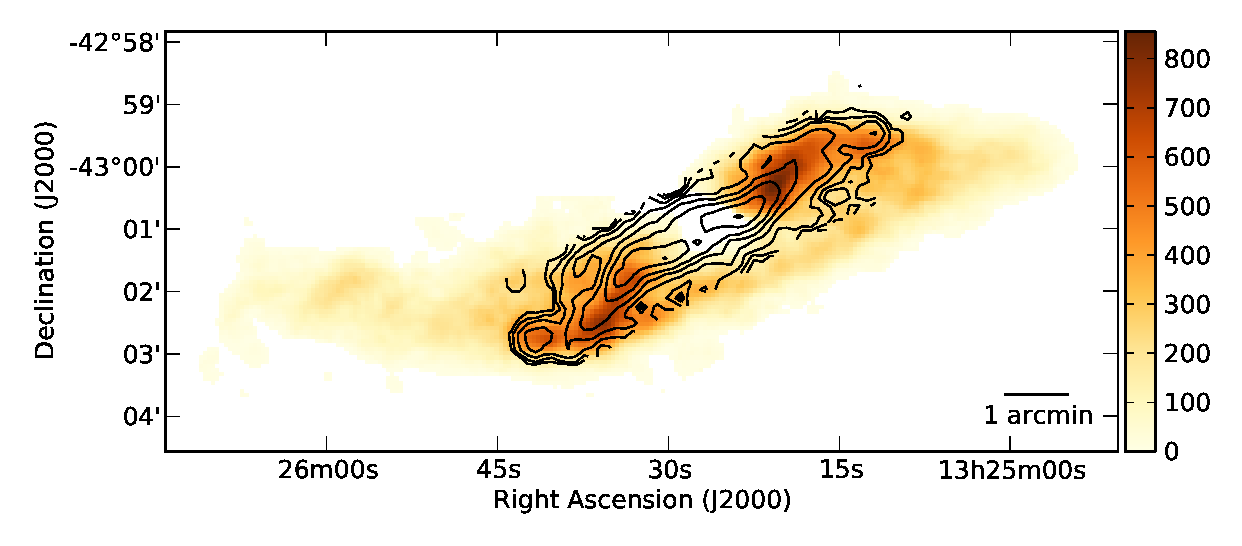
\includegraphics[width=\columnwidth]{ch2/Fig2_CenA_gas_obs}
\caption[H\textsc{i} map of the disc region of Cen~A overlaid with CO~$J=3-2$ contours]{H\textsc{i} map of the disc region of Cen~A in units of $10^{19}$~cm$^{-2}$ from \citet[][; colourscale]{2010A&A...515A..67S}, with a beam of 19~arcsec.  JCMT CO~$J=3-2$ contours with a resolution of 14.5~arcsec are overlaid in black.  CO contour levels are 0.4, 0.8, 1.6, 3.2,\ldots,25.6 and 38.4~K~km~s$^{-1}$, where the temperature units are $T_{\mathrm{A}}$*.}
\label{fig:co_map}
\end{figure*}

\subsection{Ancillary Data}\label{subsec:Ancillary}
The H\,\textsc{i} map of Cen~A was kindly provided to us by Tom Oosterloo and previously published in \citet{2010A&A...515A..67S}.  This map has a resolution of 19\,arcsec and units of $10^{19}$~cm$^{-2}$, with a pixel scale of 4\,arcsec.  We smoothed the image to a resolution of 36\,arcsec using a Gaussian beam to match the resolution of the SPIRE 500~$\mu$m image, and regridded the image to match the 12\,arcsec pixel size.

We also have a map of the radio continuum at 1.425\,GHz, originally published as part of the \emph{IRAS} Bright Galaxy Atlas \citep{1996ApJS..103...81C}, and retrieved from the NASA Extragalactic Database (NED).  This map allows us to trace the jets extending out from the central AGN.  We convolved this radio image with a Gaussian beam and then regridded it to match the SPIRE 500~$\mu$m image.


\section{Results}\label{sec:results}
\subsection{SED Fitting}\label{subsec:sed}
To determine the dust temperatures within the disc of Cen~A, we fit the far-infrared and submm part of the spectral energy distribution (SED; 70 -- 500~$\mu$m) with a simple modified blackbody with $\beta = 2$,
\begin{equation}\label{eqn:blackbody}
 I(\nu,T) = C \times \nu^{\beta} \times B(\nu,T),
\end{equation}
where $C$ is a scaling constant to match the model to our observed fluxes.  The parameter $\beta$ originates from the dust emissivity function, $\kappa_{\nu} = \kappa_{0}(\nu/\nu_{0})^{\beta}$.

To constrain our modified blackbody fits, we created uncertainty maps for each wavelength that are a combination of the measurement uncertainty in the flux value of each pixel, the background noise in each pixel, and the calibration uncertainties for both PACS and SPIRE (see Section~\ref{subsec:Noise} for details), added in quadrature.  The value in each pixel of the resulting map is taken to be the total uncertainty for the equivalent pixel at a given wavelength.

For each pixel in the images that has a S/N~$\ge 10$ at all five \emph{Herschel} wavelengths, we fit Equation~\ref{eqn:blackbody} to our flux measurements to determine the best-fitting temperature $T$ and constant $C$ for that pixel.  An example of a SED fit for a typical pixel is shown in Figure~\ref{fig:sed}, and the pixel location is shown with a cross in Figure~\ref{fig:temp}.  We also show the global SED that was obtained by summing the flux at each wavelength within all of the pixels with good fits in Figure~\ref{fig:sed}, and fitting the resulting totals.  Note that we tested the effect of removing the 70~$\mu$m data point from our SED fit to ensure it was not forcing the curve to peak at shorter wavelengths, and that it was not from a separate thermal component of the dust \citep{2010A&A...518L..51S, 2010A&A...518L..65B, Bendo_2011_submit}.  We found that the 70~$\mu$m flux falls on the best-fit curves within uncertainties for these tests and thus we use all five wavelengths in our fitting routine.  We then create a map of the dust temperature where pixels with poor chi-squared fits at the 95~percent confidence level have been masked out.  In general the pixels with poor fits coincide with those where non-thermal radiation is making a significant contribution to the flux at 500~$\mu$m. The temperature map is presented in Figure~\ref{fig:temp}, with 500~$\mu$m contours overlaid to point out the location of the non-thermal emission.  The temperature is about 30~K near the central AGN region, and then smoothly falls off to about 20~K in the outer disc, and the average temperature throughout the entire region is approximately ($21.8 \pm 0.3$)~K.
\begin{figure}
 \centering
 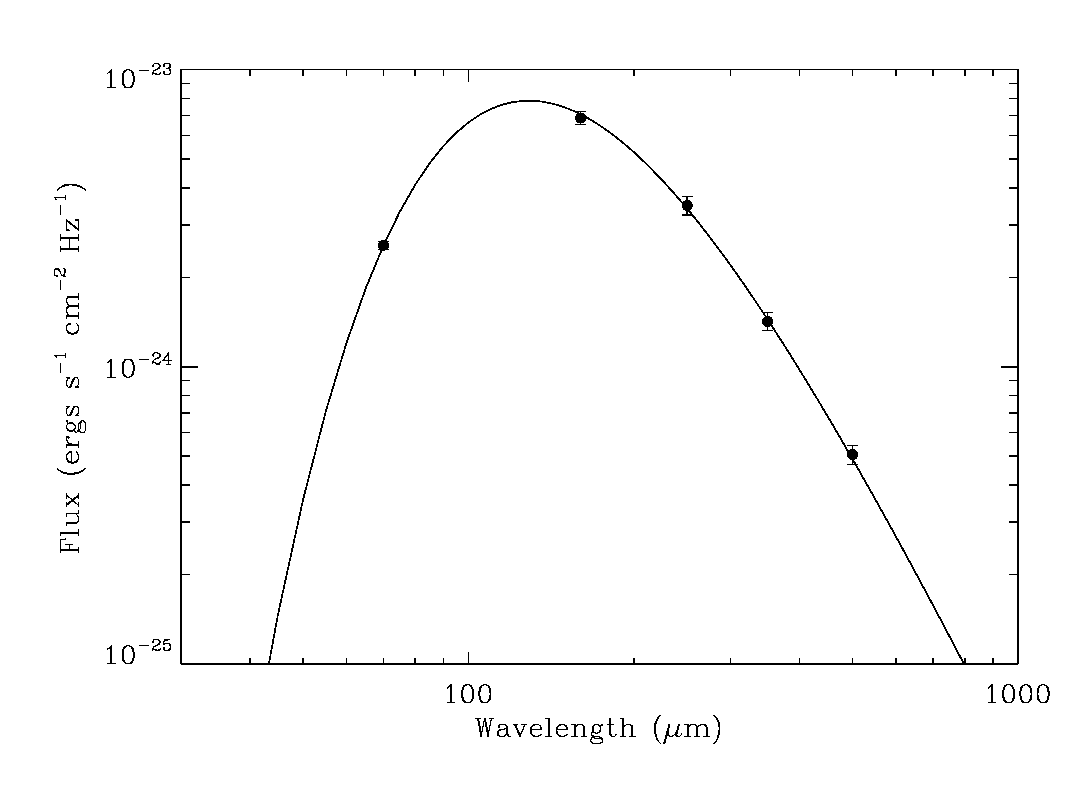
\includegraphics[width=12.0cm]{ch2/Fig3a_CenA_example_SED}
 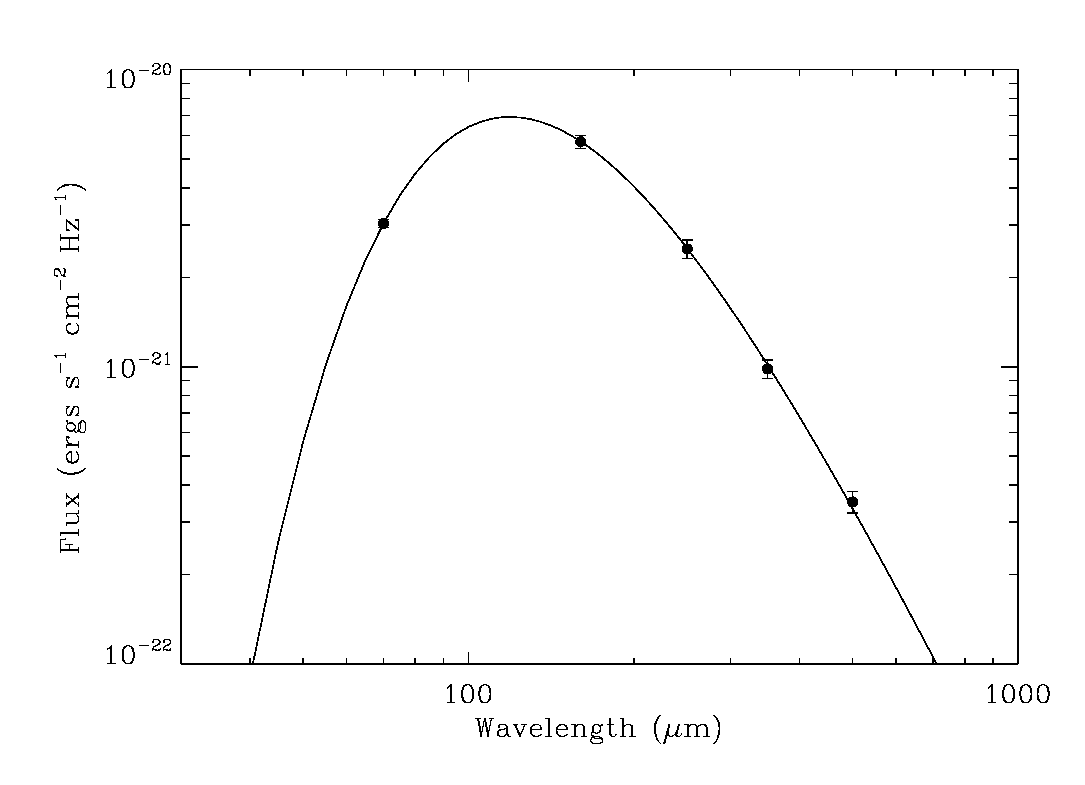
\includegraphics[width=12.0cm]{ch2/Fig3b_CenA_global_sed}
\caption[Spectral energy distributions modelled by a modified blackbody for a typical pixel and the entire disc in Centaurus~A]{Top: the SED for a typical pixel (pixel location shown as a cross in Figure~\ref{fig:temp}).  The best-fitting modified blackbody is shown as a solid line, while our measured flux values are represented by the data points. Bottom: a global SED for the entire disc, consisting of all pixels contributing to the total dust mass (see Section~\ref{subsec:dust}).}
\label{fig:sed}
\end{figure}

\begin{figure*}
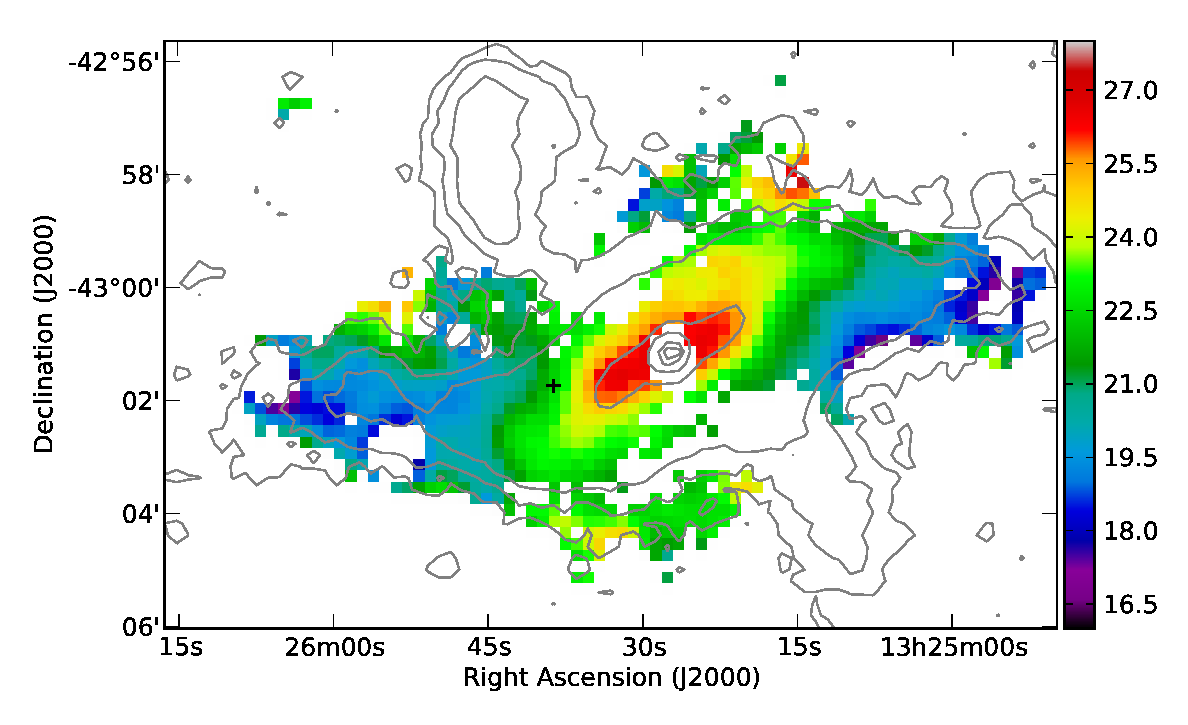
\includegraphics[width=\columnwidth]{ch2/Fig4_CenA_temp_map}
\caption[Temperature map of the dust disc of Centaurus~A]{Temperature map of the dust disc of Cen~A (colour scale), in units of degrees Kelvin.  Contours of the 500~$\mu$m SPIRE map are shown in grey for reference.  The contours for the 500~$\mu$m image are 0.0139, 0.0347, 0.0694, 0.347, 0.694, 1.39, 2.78, 4.17 and 4.86~mJy~arcsec$^{-2}$.  The black cross is the location of the pixel for which the best-fitting SED is shown in Figure~\ref{fig:sed}. Note that the central region does not have any reasonable fits due to the non-thermal emission present in the 350 and 500~$\mu$m maps.}
\label{fig:temp}
\end{figure*}

We have also tried allowing both $\beta$ and temperature to vary in Equation~\ref{eqn:blackbody}, to investigate if the model fits to our data improve.  While there is some small variation in $\beta$ throughout the disc, these deviations are small and the average value of $\beta$ is $2.07 \pm 0.07$.  Furthermore, there are no obvious trends in the variation of $\beta$ with radius.  Thus, the results of our test are consistent with our one parameter fit, giving us confidence in our fixed $\beta$ fits.

We evaluated the uncertainty on the dust temperature by implementing a monte carlo algorithm on our modified blackbody fitting routine.  For each wavelength, an artificial flux value lying within the uncertainty bounds of our observed measured flux value is generated randomly using a Gaussian number generator.  Then we run the modified blackbody fitting routine on the simulated dataset and extract the temperature and constant for the best fitting function corresponding to that dataset.  This process of creating artificial data and then fitting a function to them to determine the temperature is repeated 800 times for each pixel.  We take the standard deviation of the temperature distribution for each pixel to be the uncertainty in the temperature.  This uncertainty varies throughout the map, with an average of about 1~percent per pixel.  The highest uncertainties are $5$~percent around the very edge of our map, where the signal to noise is lower for the flux maps, and we note that these uncertainties exclude the uncertainties arising from our assumed value for $\beta$ and thus emissivity.

\subsection{Dust Mass}\label{subsec:dust}
The equation we use to evaluate the dust mass at a specific frequency is
\begin{equation}\label{eqn:dust_mass}
 M_{\mathrm{dust}} = \frac{S_{\nu}D^{2}}{\kappa_{\nu} B(\nu,T)},
\end{equation}
when the monochromatic flux is optically thin.  In this expression, $S_{\nu}$ is the flux from the source, $D$ is the distance to the source, $B(\nu,T)$ is the equation for a blackbody and $\kappa_{\nu}$ is the dust emissivity.  Here we adopt a value for the dust emissivity at 250~$\mu$m, $\kappa_{250}$, of 3.98~cm$^{2}$~g$^{-1}$ from the dust model of \citet{2003ARA&A..41..241D}\footnote{These data are also available at \newline http://www.astro.princeton.edu/~draine/dust/dustmix.html}.  Substituting $\kappa_{250}$ into Equation~\ref{eqn:dust_mass}, the dust mass becomes
\begin{equation}\label{eqn:spire_dust_mass}
 M_{\mathrm{dust}} = 5.258 \times 10^{3}S_{250}\left(\mathrm{e}^{(57.58~\mathrm{K}/T)}-1\right) ~\mathrm{M}_{\odot}.
\end{equation}
We checked that the SED of Cen~A is optically thin by assuming that the pixel with the highest flux at 70~$\mu$m is a worst-case scenario in terms of optical depth $\tau$, and measured the flux in the same pixel at 250~$\mu$m.  Using the results from our SED fitting we calculate the dust mass within that pixel using Equation~\ref{eqn:spire_dust_mass}, and convert the dust mass to a dust mass surface density $\Sigma$ using the area of one 12~arcsec pixel. The optical depth at 250~$\mu$m can be calculated as $\tau_{250} = \Sigma \kappa_{250}$.  Using this method we find that $\tau_{250} \ll 1$, thus we can assume the galaxy is optically thin at 250~$\mu$m.  This method can be repeated for the other wavelengths as well.

Substituting our temperature and the SPIRE 250~$\mu$m fluxes returned by our model SED fits into Equation~\ref{eqn:spire_dust_mass}, we obtain a  pixel-by-pixel map of the dust mass, which is shown in Figure~\ref{fig:dust_mass}.  The dust mass distribution peaks toward the centre, and falls off in the outer regions.  Uncertainties range from about 3 to 30~percent with the lower uncertainties corresponding to pixels closer to the centre of the disc.  The typical uncertainty in each pixel is $\sim 5$~percent.  Summing up the individual dust masses within each pixel leads to a total dust mass in the disc of $(1.59 \pm 0.05) \times 10^{7}$~M$_{\odot}$.  As a check, we also evaluated the total dust mass using the global SED fit results, and obtain a total of $1.47 \times 10^{7}$~M$_{\odot}$.

\begin{figure*}
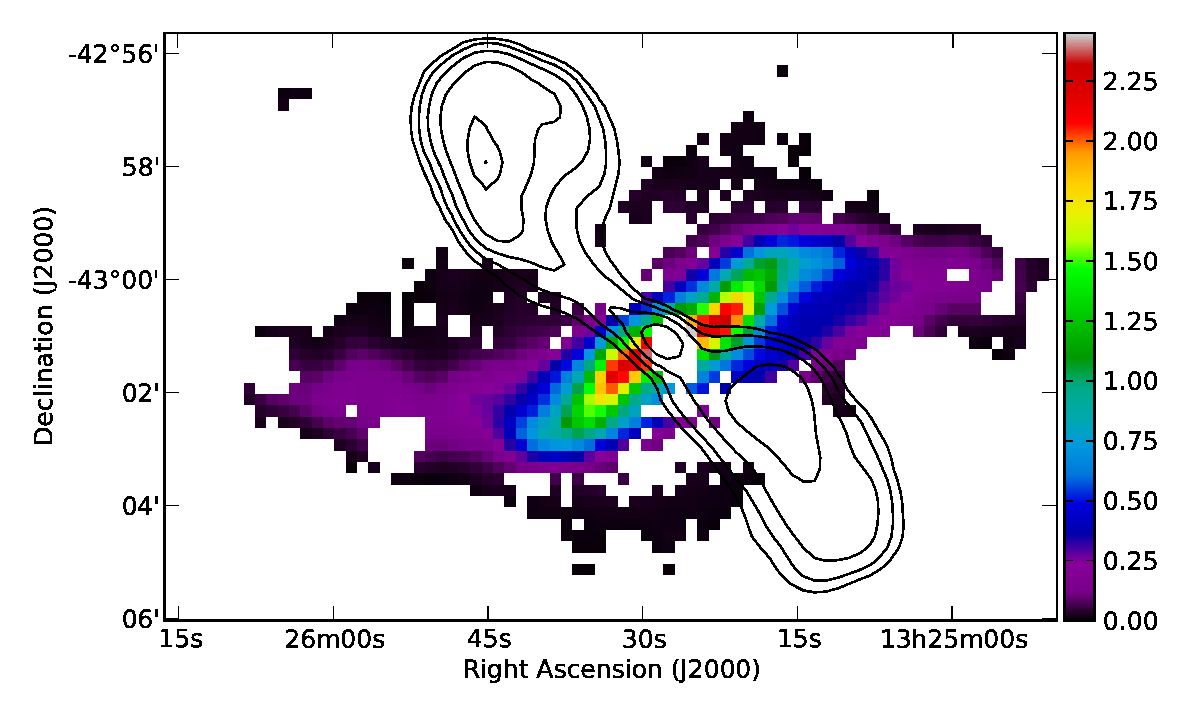
\includegraphics[width=\columnwidth]{ch2/Fig5_CenA_dust_mass}
\caption[Dust mass map of the disc of Centaurus~A]{Dust mass map of Centaurus A.  Units of the colour scale are M$_{\odot}$~pc$^{-2}$.  Contours of the 1.425~GHz radio continuum are overlaid in black to show the regions where synchrotron radiation is present.}
\label{fig:dust_mass}
\end{figure*}

\subsection{Gas Mass}\label{subsec:gas}
We convert our CO~$J=3-2$ integrated intensity map to a column density of molecular hydrogen using the following equation:
\begin{equation}\label{eqn:CO_col_density}
N_{\mathrm{H}_{2}} = \frac{\mathrm{X}_{\mathrm{CO}} I_{\mathrm{CO}(3-2)}}{\eta_{\mathrm{mb}}} \left(\frac{I_{\mathrm{CO}(3-2)}}{I_{\mathrm{CO}(1-0)}}\right)^{-1},
\end{equation}
where X$_{\mathrm{CO}}$ is the CO($J=1-0$)-H$_{2}$ conversion factor, $I_{\mathrm{CO}(3-2)}$ is the integrated intensity of the CO~$J=3-2$ emission, $\eta_{\mathrm{mb}}=0.6$ is the conversion factor from an antenna temperature $T_{\mathrm{A}}$* to a main beam temperature $T_{\mathrm{mb}}$ for the JCMT, and the factor within the brackets is the ratio of the CO~$J=3-2$ line intensity to the CO~$J=1-0$ line intensity.  Despite the additional uncertainty introduced by this line intensity ratio, we choose to use our CO~$J=3-2$ map in this analysis because of its better intrinsic resolution (14.5~arcsec) and sensitivity compared to the CO~$J=1-0$ of \citet{1990ApJ...363..451E}.  We assume a X$_{\mathrm{CO}}$ factor of $(2 \pm 1) \times 10^{20}$~cm$^{-2}$~(K~km~s$^{-1}$)$^{-1}$, typical for the Milky Way \citep{1988A&A...207....1S}, and a CO~$J=3-2$/CO~$J=1-0$ ratio of 0.3, which is a suitable ratio for the diffuse ISM as found by the JCMT Nearby Galaxies Legacy Survey \citep[NGLS;][]{2009ApJ...693.1736W}.  We note here that \citet{2009ApJ...693.1736W} and other groups from the NGLS have seen ratio variations within other galaxies by up to a factor of 2-3, which may increase our molecular gas mass uncertainties (see Section~\ref{sec:discuss} for further discussion).

Next, we convert our column density to a molecular gas mass map via
\begin{equation}\label{eqn:mol_gas_mass}
M_{\mathrm{H}_{2}} = A_{\mathrm{pix}} N_{\mathrm{H}_{2}} m_{\mathrm{H}_{2}}
\end{equation}
with $A_{\mathrm{pix}}$ the area of one pixel (12~arcsec~$\times$~12~arcsec) at the distance of Cen~A, and $m_{\mathrm{H}_{2}}$ the mass of one molecular hydrogen atom.  The total mass of molecular hydrogen, over the entire coverage of our map, is $(1.42 \pm 0.15) \times 10^{9}$~M$_{\odot}$, where we have excluded uncertainty contributions from the assumed CO~$J=3-2$/CO~$J=1-0$ ratio.

Following the same method we also convert the units of the H\textsc{i} map (Figure~\ref{fig:co_map}) to units of mass.  Then the molecular gas mass and atomic gas mass maps are combined in such a way that in regions where we have coverage for both H\textsc{i} and H$_{2}$, the total gas mass is a sum of the two, and for the remaining regions the mass is from H\textsc{i} or H$_{2}$ alone.  We then multiply the resulting map by 1.36 to obtain the total gas mass, including helium.  Summing over all pixels, we find a total gas mass of $(2.7 \pm 0.2)\times 10^{9}$~M$_{\odot}$.  Our map of the total gas is presented in Figure~\ref{fig:gas}, and covers about half of the area for which we have dust mass measurements.

\begin{figure*}
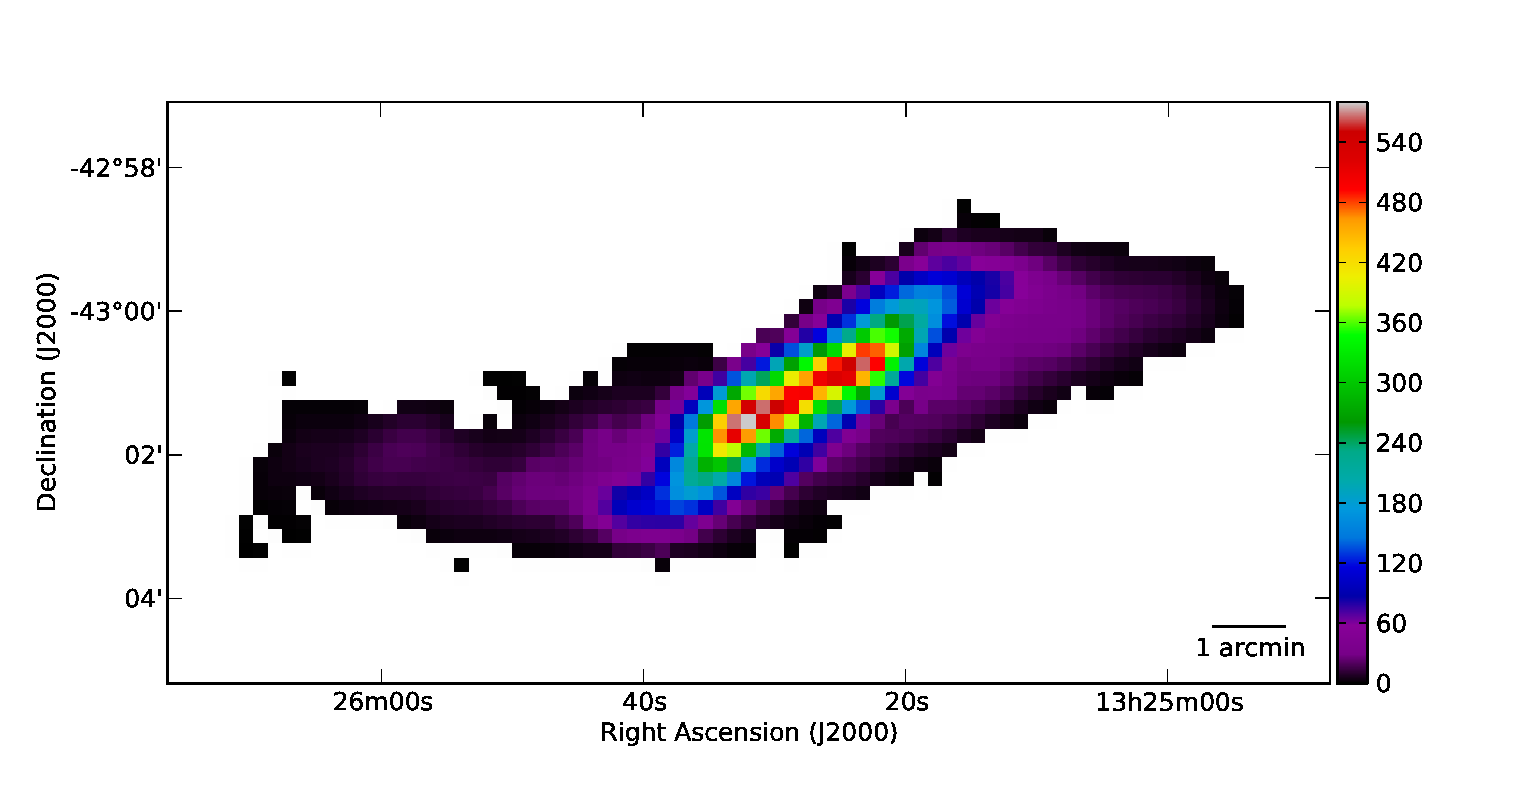
\includegraphics[width=\columnwidth]{ch2/Fig6_CenA_tot_gas_mass}
\caption[The total gas mass distribution of the disc of Centaurus~A]{The total gas mass distribution of the disc of Cen~A.  This map includes both the H\textsc{i} mass distribution, as well as the H$_{2}$ mass, where we have coverage for it, and has been multiplied by 1.36 to account for helium as well.  Units for the colour scale are M$_{\odot}$~pc$^{-2}$.}
\label{fig:gas}
\end{figure*}


\subsection{The Gas-to-Dust Mass Ratio}\label{subsec:gas2dust}
We present the gas-to-dust mass ratio in Figure~\ref{fig:g2d}, which covers all pixels for which we have both a gas mass and a dust mass.  The box outlined in black shows the region that has coverage both in H\textsc{i} and H$_{2}$, which is 10~arcmin~$\times$~2~arcmin in area.  As is seen in this figure, the majority of the disc has a gas-to-dust mass ratio similar to that of the Galaxy with an average value of $103 \pm 8$; the Galactic value varies from about 120 \citep{2001ApJ...554..778L} to $\sim 160$ \citep{2004ApJS..152..211Z} to $\sim$180 \citep[][and references therein]{2007ApJ...663..866D}.  Interestingly, the gas-to-dust mass ratio increases to a significantly higher value of almost 300 in regions closest to the AGN.  Typical uncertainties in this ratio are about 10~percent.  We also present the average gas-to-dust mass ratio as a function of distance from the centre of Cen~A along a position angle of 30~deg north of west in Figure~\ref{fig:g2d_radial}. This plot emphasizes the radial trend of the gas-to-dust mass ratio along the disc. In other galaxies such as those from the SINGS survey, the gas-to-dust mass ratio varies from $\sim 136$ to $\sim 453$ \citep{2007ApJ...663..866D}.  We discuss the possible origin of this high central gas-to-dust mass ratio below.
\begin{figure*}
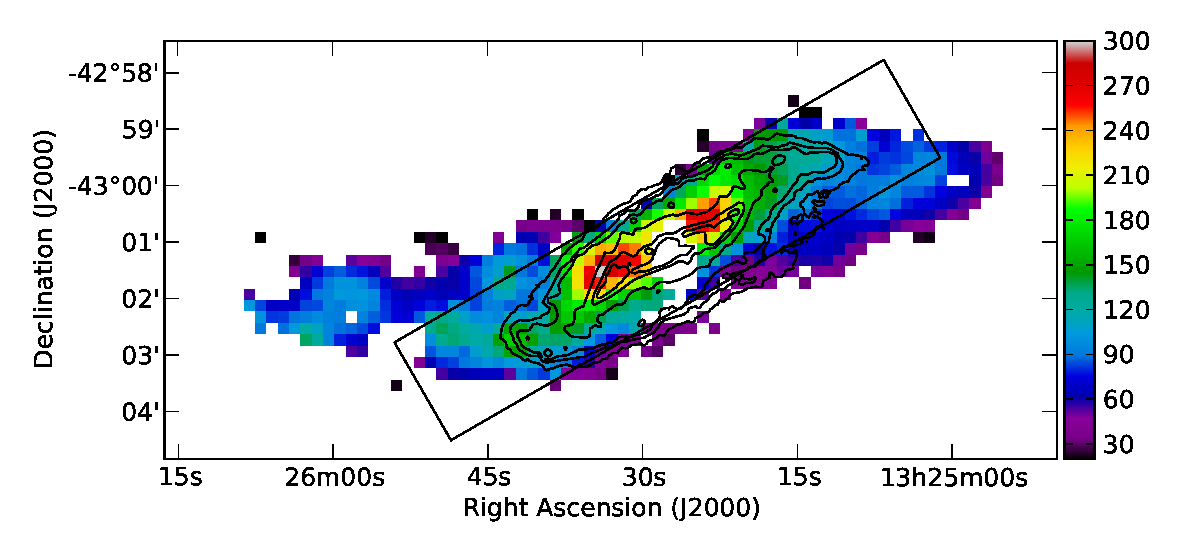
\includegraphics[width=\columnwidth]{ch2/Fig7_CenA_G2D}
\caption[Gas-to-dust mass ratio of Centaurus~A]{Gas-to-dust mass ratio of Centaurus~A (colourscale), with PACS 70~$\mu$m contours (at original resolution) overlaid in black.  Contour levels are 0.75, 1.5, 2.5, 7.5, 20, and 37.5~mJy~arcsec$^{-2}$.  The box shown in black highlights the region in the disc for which the gas contribution is from H\textsc{i} and H$_{2}$, and is 10~arcmin~$\times$~2~arcmin in size.}
\label{fig:g2d}
\end{figure*}

\begin{figure}
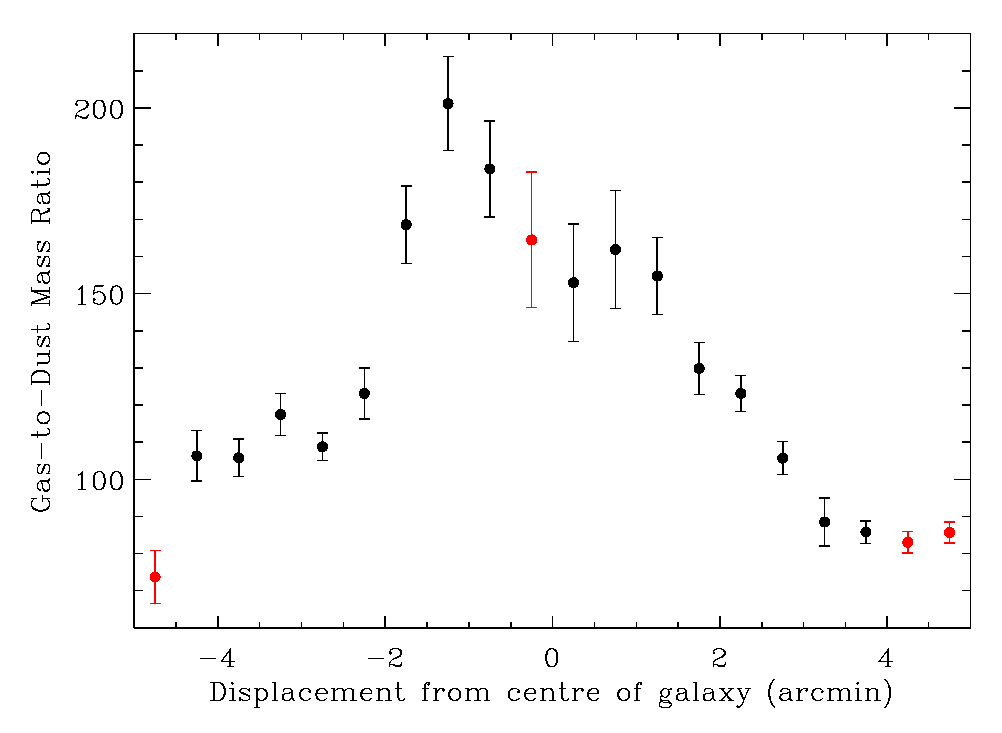
\includegraphics[width=\columnwidth]{ch2/Fig8_CenA_G2D_radial_plot}
\caption[A radial plot of the average gas-to-dust mass ratio along the major axis of Centaurus~A]{A radial plot of the average gas-to-dust mass ratio along the major axis of Cen~A with a position angle of 30~deg north of west.  We measured the average gas-to-dust mass ratio value within 20 bins along this position-angle, each measuring 2~arcmin~$\times$~0.5~arcmin in size.  The red data points represent the bins in which we had at most 10 good pixels out of a possible 25, and therefore are not as well sampled as those shown in black.}
\label{fig:g2d_radial}
\end{figure}


\section{Discussion}\label{sec:discuss}
Our total dust mass of $(1.59 \pm 0.05) \times 10^{7}$~M$_{\odot}$ is comparable to other published numbers for Cen~A in the literature; however, we note that this value is likely a lower limit as regions where non-thermal emission contaminates the dust continuum had poor model fits.  Several publications have used two-component modified blackbody modelling combined with far-infrared and submm observations to derive a dust mass for Cen~A.  \citet{2002ApJ...565..131L} used a wavelength range of 60--850~$\mu$m for their SED fit and found a total mass of $2.6 \times 10^{6}$~M$_{\odot}$ (adjusting for our distance) within an elliptical region 120~arcsec~$\times$~450~arcsec in size, but excluding the unresolved core at the centre.  Since this ellipse covers a similar area to our observations, the discrepancy is likely due to an inadequate chop throw in the \citet{2002ApJ...565..131L} 850~$\mu$m dataset, leading to difficulties quantifiying the background.  Our observations show faint emission at 500~$\mu$m extending beyond the 120~arcsec chop throw the authors used, and oversubtracting the background will lead to a lower dust mass estimate.  \citet{2008A&A...490...77W} studied the submm continuum using LABOCA 870~$\mu$m data and combining these data with fluxes spanning 25--870~$\mu$m they found a higher mass of $2.2 \times 10^{7}$~M$_{\odot}$.  They subtract the flux contribution of the unresolved core from the total flux prior to estimating the dust, but do caution that they may not have removed all of the non-thermal emission arising from the radio jet.

The gas mass we have obtained from our H$_{2}$ map alone is $(1.42 \pm 0.15) \times 10^{9}$~M$_{\odot}$, including the central region which we masked out for our dust fitting.  \citet{1990ApJ...363..451E} determined a molecular gas mass of $1.9 \times 10^{8}$~M$_{\odot}$, after we adjust their result for our assumed X$_{\mathrm{CO}}$ factor and distance.  In addition, \citet{2010PASA...27..463M} suggests the total molecular gas mass is $4 \times 10^{8}$~M$_{\odot}$ based on observations of \citet{1990ApJ...363..451E} and \citet{1992ApJ...391..121Q}.  Our molecular gas mass is thus higher than those values previously published; this is likely due to the improved sensitivity of our observations.  The molecular gas mass is about twice the atomic mass of $4.9 \times 10^{8}$~M$_{\odot}$ \citep{2010A&A...515A..67S}.

The high gas-to-dust mass ratio towards the central AGN is a most interesting result.  Several studies of spiral galaxies have found that the gas-to-dust mass ratio is not constant throughout the disc, but rather decreases with decreasing distance from the centre of the galaxy \citep[e.g.][]{2009ApJ...701.1965M,2010MNRAS.402.1409B,2011arXiv1106.0618M}, in contrast to what we have found here.  We have made a rough estimate of the CO~$J=3-2$/CO~$J=1-0$ ratio throughout the central disc using the CO~$J=1-0$ map of \citet{1990ApJ...363..451E} to check if our assumption of 0.3 for this ratio is valid in the centremost regions of the disc.  Our calculations show an average value of 0.35, and more importantly, they show no significant variation with radius.  Furthermore, looking at Figure~\ref{fig:g2d} we see that there is a smooth transition of the gas-to-dust mass ratio between the H$_{2}$-dominated region to the H\textsc{i}-dominated region in the outer disc, which also suggests CO excitation is not the primary cause of the high gas-to-dust mass ratio.

The X$_{\mathrm{CO}}$ factor is one variable that might affect the gas-to-dust mass ratio if it is not constant throughout the disc.  We have assumed the Galactic value for our calculations; however, studies have shown that this conversion factor can vary with metallicity \citep{1995ApJ...448L..97W, 1997A&A...328..471I, 2000mhs..conf..293I, 2000MNRAS.317..649B, 2003A&A...397...87I, 2004A&A...422L..47S, 2005A&A...438..855I, 2011ApJ...737...12L}.  If the metallicity decreases as a function of radius within Cen~A, we would require a larger conversion factor at larger radii, which in turn would increase the gas-to-dust mass ratio farther out in the disc, potentially bringing it up to a similar value as that in the centre.  Alternatively, the X$_{\mathrm{CO}}$ factor can be smaller by up to a factor of $\sim 4$ for starbursting galaxies \citep{1998ApJ...507..615D}.  This effect could reduce the gas-to-dust mass ratio in regions of strong star forming activity; however, the total far-infrared luminosity for Cen~A is $\le 10^{10}~L_{\odot}$, while the X$_{\mathrm{CO}}$ conversion factor is typically affected at luminosities greater than $\sim 10^{11}~L_{\odot}$ \citep[e.g.][]{1993ApJ...414L..13D, 1997ApJ...478..144S}.

One possibility is that dust is being destroyed by the jets extending out in either direction from the AGN.  It is plausible that some of the dust grains are being destroyed by the AGN either through dust sputtering or through shocks.  The total X-ray luminosity of the AGN of Cen~A is $8 \times 10^{42}$~erg~s$^{-1}$ \citep{2011ApJ...733...23R}, which is comparable in X-ray luminosity to the AGN found in M87 \citep{2006A&A...459..353W}.  It might be possible for these photons to deplete the dust in the surrounding ISM.  In support of this scenario, \citet{2010A&A...518L..53B} did not detect thermal dust emission in M87, which also contains a jet.

It is also possible that the dust is entrained in the jets of Cen~A.  \citet{2010A&A...518L..66R} found a dusty halo surrounding the starbursting galaxy M82 using \emph{Herschel} observations.  They considered entrainment by a galactic wind as a possible explanation even though they finally concluded that the origin was likely due to tidal interactions.  We cannot rule out entrainment by galactic winds as a possibility for Cen~A.  Unfortunately, we cannot probe close enough to the jets to further investigate this assumption due to our limited resolution and the non-thermal emission component.

Alternatively, a larger gas reservoir in the centre could also increase the gas-to-dust mass ratio.  This would require dust-poor gas falling onto the disc and being funneled toward the centre.  However, if this was the case, we would likely have found a high gas-to-dust mass ratio throughout the disc and not concentrated toward the innermost part of the disc.  It also does not seem plausible for the gas to be migrating through the disc faster than the dust.

Interestingly, there is a large ring of material that is seen in the mid- and far-infrared close to the regions in which we see a high gas-to-dust mass ratio.  \citet{1999A&A...341..667M} first noticed the `S' shaped structure with ISOCAM observations at 7 and 15~$\mu$m, and postulated that this structure was a bar at the centre of the galaxy.  Later, observations \citep{2002ApJ...565..131L,2006ApJ...645.1092Q} supported a tilted ring scenario to explain the structure observed.  Our \emph{Herschel} observations at 70~$\mu$m also show emission from this ring (Figure~\ref{fig:Herschel_maps2}), and in fact, the high gas-to-dust mass ratio appears to correspond with the 70~$\mu$m contours of the ring, as shown in Figure~\ref{fig:g2d}.  The models by \citet{2006ApJ...645.1092Q} suggest that there is a deficit in the dust distribution at radii less than about 50~arcsec ($\sim 920$~pc).  This is at a similar radius to our observed high gas-to-dust mass ratio.  A dust deficit throughout $r \le 50$~arcsec might seem less likely to be related to the AGN and is perhaps better related to star formation activity.  Observations probing closer to the nucleus are necessary to determine if the gas-to-dust mass ratio remains high or increases further as we approach the AGN.

\section{Conclusions}\label{sec:conclusions2}
We have presented new observations of the dust continuum from the PACS and SPIRE instruments on board the \emph{Herchel Space Observatory} at 70, 160, 250, 350 and 500~$\mu$m.  In addition, we present new data tracing the CO~$J=3-2$ transition taken with the HARP-B instrument mounted on the JCMT.  We have used these data to probe the interstellar medium within the disc of Centaurus~A on a pixel-by-pixel basis. We observe the ring of emission at 70~$\mu$m previously reported at infrared and submm wavelengths, while our 500~$\mu$m (and to some extent the 350~$\mu$m) images show detections of the non-thermal continuum emission previously reported at 870~$\mu$m by \citet{2008A&A...490...77W}.

We model the dust spectral energy distribution using a single component modified blackbody, and find temperatures of $\le 30$~K in the centre that decrease with radius.  Using the temperature map, we find the total dust mass to be $(1.59 \pm 0.05) \times 10^{7}$~M$_{\odot}$.  The total gas mass is $(2.7 \pm 0.2)\times 10^{9}$~M$_{\odot}$, and combining the dust and gas masses we have produced a gas-to-dust mass ratio map.  The average gas-to-dust mass ratio is approximately $103 \pm 8$, similar to that of the Milky Way, with an interesting peak to about 275 towards the centre of the galaxy.  After exploring several possible scenarios to explain the high gas-to-dust mass ratio, the most appealing one is that of a correspondance between the high gas-to-dust mass ratio and the ring about 1~kpc in size, which is best fit by a warped tilted ring model by \citet{2006ApJ...645.1092Q} that consists of a deficit of dusty material inwards of the ring.  The deficit of dust may be due to X-ray emission from the central AGN destroying the dust grains or due to the jets removing dust from the centre of the galaxy.

\section*{Acknowledgments}
The research of C.~D.~W. is supported by the Natural Sciences and Engineering Research Council of Canada and the Canadian Space Agency.  PACS has been developed by a consortium of institutes led by MPE (Germany) and including UVIE (Austria); KU Leuven, CSL, IMEC (Belgium); CEA, LAM (France); MPIA (Germany); INAF-IFSI/OAA/OAP/OAT, LENS, SISSA (Italy); IAC (Spain). This development has been supported by the funding agencies BMVIT (Austria), ESA-PRODEX (Belgium), CEA/CNES (France), DLR (Germany), ASI/INAF (Italy), and CICYT/MCYT (Spain).  SPIRE has been developed by a consortium of institutes led by Cardiff University (UK) and including Univ. Lethbridge (Canada); NAOC (China); CEA, LAM (France); IFSI, Univ. Padua (Italy); IAC (Spain); Stockholm Observatory (Sweden); Imperial College London, RAL, UCL-MSSL, UKATC, Univ. Sussex (UK); and Caltech, JPL, NHSC, Univ. Colorado (USA). This development has been supported by national funding agencies: CSA (Canada); NAOC (China); CEA, CNES, CNRS (France); ASI (Italy); MCINN (Spain); SNSB (Sweden); STFC and UKSA (UK); and NASA (USA).  HIPE is a joint development by the Herschel Science Ground Segment Consortium, consisting of ESA, the NASA Herschel Science Center, and the HIFI, PACS and SPIRE consortia.  The James Clerk Maxwell Telescope is operated by The Joint Astronomy Centre on behalf of the Science and Technology Facilities Council of the United Kingdom, the Netherlands Organisation for Scientific Research, and the National Research Council of Canada. This research has made use of the NASA/IPAC Extragalactic Database (NED) which is operated by the Jet Propulsion Laboratory, California Institute of Technology, under contract with the National Aeronautics and Space Administration.  This research made use of APLpy, an open-source plotting package for Python hosted at http://aplpy.github.com.  T.~J.~P. thanks the anonymous referee for providing constructive feedback about this work.



%% Commands to initiate bibliography:
\begin{thebibliography}{}
\bibitem[\protect\citeauthoryear{Auld et al.}{2012}]{Auld_2011_submit} Auld R. et al., 2012, \mnras, 420, 1882
\bibitem[\protect\citeauthoryear{Baes et al.}{2010}]{2010A&A...518L..53B} Baes M. et al., 2010, \aap, 518, L53
\bibitem[\protect\citeauthoryear{Barone et al.}{2000}]{2000MNRAS.317..649B} Barone L.~T., Heithausen A., H{\"u}ttemeister S., Fritz T., Klein U., 2000, \mnras, 317, 649
\bibitem[\protect\citeauthoryear{Bendo et al.}{2010a}]{2010A&A...518L..65B} Bendo G.~J. et al., 2010a, \aap, 518, L65
\bibitem[\protect\citeauthoryear{Bendo et al.}{2010b}]{2010MNRAS.402.1409B} Bendo G.~J. et al., 2010b, \mnras, 402, 1409
\bibitem[\protect\citeauthoryear{Bendo et al.}{2012}]{Bendo_2011_submit} Bendo G.~J. et al., 2012, \mnras, 419, 1833
\bibitem[\protect\citeauthoryear{Bregman, Hogg \& Roberts}{Bregman et al.}{1992}]{1992ApJ...387..484B} Bregman J.~N., Hogg D.~E., Roberts M.~S., 1992, \apj, 387, 484
\bibitem[\protect\citeauthoryear{Bregman et al.}{1998}]{1998ApJ...499..670B} Bregman J.~N., Snider B.~A., Grego L., Cox C.~V., 1998, \apj, 499, 670
\bibitem[\protect\citeauthoryear{Condon et al.}{1996}]{1996ApJS..103...81C} Condon J.~J., Helou G., Sanders D.~B., Soifer B.~T., 1996, \apjs, 103, 81
\bibitem[\protect\citeauthoryear{Currie et al.}{2008}]{2008ASPC..394..650C} Currie M.~J., Draper P.~W., Berry D.~S., Jenness T., Cavanagh B., Economou F., 2008, in Argyle R.~W., Bunclark P.~S., Lewis J.~R., eds, ASP Conf. Ser. Vol. 394, Astronomical Data Analysis Software and Systems XVII, Astron. Soc. Pac., San Francisco, p. 650
\bibitem[\protect\citeauthoryear{Downes \& Solomon}{1998}]{1998ApJ...507..615D} Downes D., Solomon P.~M., 1998, \apj, 507, 615
\bibitem[\protect\citeauthoryear{Downes, Solomon \& Radford}{1993}]{1993ApJ...414L..13D} Downes D., Solomon P.~M., Radford, S.~J.~E., 1993, \apjl, 414, L13
\bibitem[\protect\citeauthoryear{Draine}{2003}]{2003ARA&A..41..241D} Draine B.~T., 2003, \araa, 41, 241
\bibitem[\protect\citeauthoryear{Draine et al.}{2007}]{2007ApJ...663..866D} Draine B.~T. et al., 2007, \apj, 663, 866
\bibitem[\protect\citeauthoryear{Eckart et al.}{1990a}]{1990ApJ...363..451E} Eckart A., Cameron M., Rothermel H., Wild W., Zinnecker H., Rydbeck G., Olberg M., Wiklind T., 1990a, \apj, 363, 451
\bibitem[\protect\citeauthoryear{Eckart et al.}{1990b}]{1990ApJ...365..522E} Eckart A., Cameron M., Genzel R., Jackson J.~M., Rothermel H., Stutzki J., Rydbeck G., Wiklind T., 1990b, \apj, 365, 522
\bibitem[\protect\citeauthoryear{Griffin et al.}{2010}]{2010A&A...518L...3G} Griffin M.~J. et al., 2010, \aap, 518, L3
\bibitem[\protect\citeauthoryear{Harris}{2010}]{2010PASA...27..475H} Harris G.~L.~H., 2010, \pasa, 27, 475
\bibitem[\protect\citeauthoryear{Harris, Rejkuba \& Harris}{Harris et al.}{2010}]{2010PASA...27..457H} Harris G.~L.~H., Rejkuba M., Harris W.~E., 2010, \pasa, 27, 457
\bibitem[\protect\citeauthoryear{Huchtmeier}{1994}]{1994A&A...286..389H} Huchtmeier W.~K., 1994, \aap, 286, 389
\bibitem[\protect\citeauthoryear{Huchtmeier, Sage \& Henkel}{Huchtmeier et al.}{1995}]{1995A&A...300..675H} Huchtmeier W.~K., Sage L.~J., Henkel C., 1995, \aap, 300, 675
\bibitem[\protect\citeauthoryear{Israel}{1997}]{1997A&A...328..471I} Israel F.~P., 1997, \aap, 328, 471
\bibitem[\protect\citeauthoryear{Israel}{1998}]{1998A&ARv...8..237I} Israel F.~P., 1998, \aapr, 8, 237
\bibitem[\protect\citeauthoryear{Israel}{2000}]{2000mhs..conf..293I} Israel F.~P., 2000, in Combes F., Pineau Des Forets G., eds, Cambridge Contemporary Astrophysics Vol. xix,  Molecular Hydrogen in Space, Cambridge University Press, Cambridge, p. 293
\bibitem[\protect\citeauthoryear{Israel}{2005}]{2005A&A...438..855I} Israel F.~P., 2005, \aap, 438, 855
\bibitem[\protect\citeauthoryear{Israel et al.}{2003}]{2003A&A...397...87I} Israel F.~P., Baas F., Rudy R.~J., Skillman E.~D., Woodward C.~E., 2003, \aap, 397, 87
\bibitem[\protect\citeauthoryear{Knapp, Turner \& Cunniffe}{Knapp et al.}{1985}]{1985AJ.....90..454K} Knapp G.~R., Turner E.~L., Cunniffe P.~E., 1985, \aj, 90, 454
\bibitem[\protect\citeauthoryear{Leeuw et al.}{2002}]{2002ApJ...565..131L} Leeuw L.~L., Hawarden T.~G., Matthews H.~E., Robson E.~I., Eckart A., 2002, \apj, 565, 131
\bibitem[\protect\citeauthoryear{Leeuw et al.}{2008}]{2008ApJ...677..249L} Leeuw L.~L., Davidson J., Dowell C.~D., Matthews H.~E., 2008, \apj, 677, 249
\bibitem[\protect\citeauthoryear{Leroy et al.}{2011}]{2011ApJ...737...12L} Leroy A.~K. et al., 2011, \apj, 737, 12
\bibitem[\protect\citeauthoryear{Li \& Draine}{2001}]{2001ApJ...554..778L} Li A., Draine B.~T., 2001, \apj, 554, 778
\bibitem[\protect\citeauthoryear{Magrini et al.}{2011}]{2011arXiv1106.0618M} Magrini L. et al., 2011, \aap, 535, 13
\bibitem[\protect\citeauthoryear{Mirabel et al.}{1999}]{1999A&A...341..667M} Mirabel I.~F. et al., 1999, \aap, 341, 667
\bibitem[\protect\citeauthoryear{Morganti}{2010}]{2010PASA...27..463M} Morganti R., 2010, \pasa, 27, 463
\bibitem[\protect\citeauthoryear{Morganti et al.}{1999}]{1999ASPC..163...84M} Morganti R., Oosterloo T., Sadler E.~M., Vergani D., 1999, in Carral P., Cepa J., eds, ASP Conf. Ser. Vol. 163, Star Formation in Early Type Galaxies, Astron. Soc. Pac., San Francisco, p. 84
\bibitem[\protect\citeauthoryear{Morganti et al.}{2006}]{2006MNRAS.371..157M} Morganti R. et al., 2006, \mnras, 371, 157
\bibitem[\protect\citeauthoryear{Morganti et al.}{2008}]{2008A&A...485L...5M} Morganti R., Oosterloo T., Struve C., Saripalli L., 2008, \aap, 485, L5
\bibitem[\protect\citeauthoryear{M{\"u}ller et al.}{2011}]{PACS_cc_2011} M{\"u}ller T., Okumura K., Klaas U., 2011, PICC-ME-TN-038, available from the ESA \emph{Herschel} Science Centre
\bibitem[\protect\citeauthoryear{Mu{\~n}oz-Mateos et al.}{2009}]{2009ApJ...701.1965M} Mu{\~n}oz-Mateos J.~C. et al., 2009, \apj, 701, 1965
\bibitem[\protect\citeauthoryear{Nguyen et al.}{2010}]{2010A&A...518L...5N} Nguyen H.~T. et al., 2010, \aap, 518, L5
\bibitem[\protect\citeauthoryear{Ott}{2010}]{2010ASPC..434..139O} Ott S., 2010, in Mizumoto Y., Morita K.-I., Ohishi M., eds, ASP Conf. Ser. Vol. 434, Astronomical Data Analysis Software and Systems XIX, Astron. Soc. Pac., San Francisco, p. 139
\bibitem[\protect\citeauthoryear{PACS Observer's Manual}{2011}]{PACS_OM} PACS Observer's Manual, 2011, HERSCHEL-HSC-DOC-0832, available from the ESA \emph{Herschel} Science Centre
\bibitem[\protect\citeauthoryear{Phillips et al.}{1987}]{1987ApJ...322L..73P} Phillips T.~G. et al., 1987, \apj, 322, L73
\bibitem[\protect\citeauthoryear{Pilbratt et al.}{2010}]{2010A&A...518L...1P} Pilbratt G.~L. et al., 2010, \aap, 518, L1
\bibitem[\protect\citeauthoryear{Poglitsch et al.}{2010}]{2010A&A...518L...2P} Poglitsch A. et al., 2010, \aap, 518, L2
\bibitem[\protect\citeauthoryear{Quillen et al.}{1992}]{1992ApJ...391..121Q} Quillen A.~C., de Zeeuw P.~T., Phinney E.~S., Phillips T.~G., 1992, \apj, 391, 121
\bibitem[\protect\citeauthoryear{Quillen et al.}{2006}]{2006ApJ...645.1092Q} Quillen A.~C., Brookes M.~H., Keene J., Stern D., Lawrence C.~R., Werner M.~W., 2006, \apj, 645, 1092
\bibitem[\protect\citeauthoryear{Rothschild et al.}{2011}]{2011ApJ...733...23R} Rothschild R.~E., Markowitz A., Rivers E., Suchy S., Pottschmidt K., Kadler M., M{\"u}ller C., Wilms J., 2011, \apj, 733, 23
\bibitem[\protect\citeauthoryear{Roussel}{2013}]{Roussel_2011_submit} Roussel H., 2013, \pasp, preprint (arXiv:1205.2576)
\bibitem[\protect\citeauthoryear{Roussel et al.}{2010}]{2010A&A...518L..66R} Roussel H. et al., 2010, \aap, 518, L66
\bibitem[\protect\citeauthoryear{Rydbeck et al.}{1993}]{1993A&A...270L..13R} Rydbeck G., Wiklind T., Cameron M., Wild W., Eckart A., Genzel R., Rothermel H., 1993, \aap, 270, L13
\bibitem[\protect\citeauthoryear{Schiminovich et al.}{1994}]{1994ApJ...423L.101S} Schiminovich D., van Gorkom J.~H., van der Hulst J.~M., Kasow S., 1994, \apjl, 423, L101
\bibitem[\protect\citeauthoryear{Smith et al.}{2010}]{2010A&A...518L..51S} Smith M.~W.~L. et al., 2010, \aap, 518, L51
\bibitem[\protect\citeauthoryear{Smith et al.}{2012}]{Smith_2012_in_press} Smith M.~W.~L. et al., 2012, \apj, 748, 123
\bibitem[\protect\citeauthoryear{Solomon et al.}{1997}]{1997ApJ...478..144S} Solomon P.~M., Downes D., Radford S.~J.~E., Barrett J.~W., 1997, \apj, 478, 144
\bibitem[\protect\citeauthoryear{SPIRE Observers' Manual}{2011}]{SOM_2010} SPIRE Observers' Manual, 2011, HERSCHEL-HSC-DOC-0798, available from the ESA \emph{Herschel} Science Centre
\bibitem[\protect\citeauthoryear{Stickel et al.}{2004}]{2004A&A...415...95S} Stickel M., van der Hulst J.~M., van Gorkom J.~H., Schiminovich D., Carilli C.~L., 2004, \aap, 415, 95
\bibitem[\protect\citeauthoryear{Strong et al.}{1988}]{1988A&A...207....1S} Strong A.~W. et al., 1988, \aap, 207, 1
\bibitem[\protect\citeauthoryear{Strong et al.}{2004}]{2004A&A...422L..47S} Strong A.~W., Moskalenko I.~V., Reimer O., Digel S., Diehl R., 2004, \aap, 422, L47
\bibitem[\protect\citeauthoryear{Struve et al.}{2010}]{2010A&A...515A..67S} Struve C., Oosterloo T.~A., Morganti R., Saripalli L., 2010, \aap, 515, A67
\bibitem[\protect\citeauthoryear{Temi et al.}{2004}]{2004ApJS..151..237T} Temi P., Brighenti F., Mathews W.~G.. Bregman J.~D., 2004, \apjs, 151, 237
\bibitem[\protect\citeauthoryear{Thronson et al.}{1989}]{1989ApJ...344..747T} Thronson Jr. H.~A., Tacconi L., Kenney J., Greenhouse M.~A., Margulis M., Tacconi-Garman L., Young J.~S., 1989, \apj, 344, 747
\bibitem[\protect\citeauthoryear{van Gorkom et al.}{1990}]{1990AJ.....99.1781V} van Gorkom J.~H., van der Hulst J.~M., Haschick A.~D., Tubbs A.~D., 1990, \aj, 99, 1781
\bibitem[\protect\citeauthoryear{Walsh et al.}{1989}]{1989ApJ...337..209W} Walsh D.~E.~P., Knapp G.~R., Wrobel J.~M., Kim D.-W., 1989, \apj, 337, 209
\bibitem[\protect\citeauthoryear{Warren et al.}{2010}]{2010ApJ...714..571W} Warren B.~E. et al., 2010, \apj, 714, 571
\bibitem[\protect\citeauthoryear{Wei{\ss} et al.}{2008}]{2008A&A...490...77W} Wei{\ss} A., Kov{\'a}cs A., G{\"u}sten R., Menten K.~M., Schuller F., Siringo G., Kreysa E., 2008, \aap, 490, 77
\bibitem[\protect\citeauthoryear{Welch \& Sage}{2003}]{2003ApJ...584..260W} Welch G.~A., Sage L.~J., 2003, \apj, 584, 260
\bibitem[\protect\citeauthoryear{Welch, Sage \& Young}{Welch et al.}{2010}]{2010ApJ...725..100W} Welch G.~A., Sage L.~J., Young L.~M., 2010, \apj, 725, 100
\bibitem[\protect\citeauthoryear{Werner et al.}{2006}]{2006A&A...459..353W} Werner N., B{\"o}hringer H., Kaastra J.~S., de Plaa J., Simionescu A., Vink J., 2006, \aap, 459, 353
\bibitem[\protect\citeauthoryear{Wiklind, Combes \& Henkel}{Wiklind et al.}{1995}]{1995A&A...297..643W} Wiklind T., Combes F., Henkel C., 1995, \aap, 297, 643
\bibitem[\protect\citeauthoryear{Wilson}{1995}]{1995ApJ...448L..97W} Wilson C.~D., 1995, \apjl, 448, L97
\bibitem[\protect\citeauthoryear{Wilson et al.}{2009}]{2009ApJ...693.1736W} Wilson C.~D. et al., 2009, \apj, 693, 1736
\bibitem[\protect\citeauthoryear{Xilouris et al.}{2004}]{2004A&A...416...41X} Xilouris E.~M., Madden S.~C., Galliano F., Vigroux L., Sauvage M., 2004, \aap, 416, 41
\bibitem[\protect\citeauthoryear{Young, Bendo \& Lucero}{Young et al.}{2009}]{2009AJ....137.3053Y} Young L.~M., Bendo G.~J., Lucero D.~M., 2009, \aj, 137, 3053
\bibitem[\protect\citeauthoryear{Young et al.}{2011}]{2011MNRAS.414..940Y} Young L.~M. et al., 2011, \mnras, 414, 940
\bibitem[\protect\citeauthoryear{Zubko et al.}{2004}]{2004ApJS..152..211Z} Zubko V., Dwek E., Arendt R.~G., 2004, \apjs, 152, 211
\end{thebibliography}


%\bibliography{thesis_bib}
%\bibliographystyle{apj}
\pagestyle{fancy}
\headheight 20pt
\lhead{Ph.D. Thesis --- T.~J. Parkin }
\rhead{McMaster - Physics \& Astronomy}
\chead{}
\lfoot{}
\cfoot{\thepage}
\rfoot{}
\renewcommand{\headrulewidth}{0.1pt}
\renewcommand{\footrulewidth}{0.1pt}


\chapter{Regional variations in the dense gas heating and cooling in M51 from \emph{Herschel} far-infrared spectroscopy} \label{chapter3}

\thispagestyle{fancy}

\noindent T.~J. Parkin, C.~D. Wilson, M.~R.~P. Schirm, M. Baes, M. Boquien,, A. Boselli, A. Cooray, D. Cormier, K. Foyle, O.~\L. Karczewski, V. Lebouteiller, I. de~Looze, S.~C. Madden, H. Roussel, M. Sauvage, and L. Spinoglio

\vspace{1.5cm}

\noindent \emph{This article has been accepted for publication in The Astrophysical Journal, but as of the time of submission of my final thesis it has not yet been assigned a bibliographic designation.  Reproduced by permission of the American Astronomical Society.}

%%
%% M51 Herschel PACS spectroscopy paper
%% Revised Version 2
%% Last update: August 15, 2013
%%
%% Tara Parkin

%\title{Regional variations in the dense gas heating and cooling in M51 from \emph{Herschel}\footnote{\emph{Herschel} is an ESA space observatory with science instruments provided by European-led Principal Investigator consortia and with important participation from NASA.} far-infrared spectroscopy}

%\author{T.~J. Parkin\altaffilmark{2}, C.~D. Wilson\altaffilmark{2}, M.~R.~P. Schirm\altaffilmark{2}, 
%	M. Baes\altaffilmark{3}, M. Boquien\altaffilmark{4}, A. Boselli\altaffilmark{4},
%	A. Cooray\altaffilmark{5,6}, D. Cormier\altaffilmark{7}, K. Foyle\altaffilmark{2},
%	O.~\L. Karczewski\altaffilmark{8}, V. Lebouteiller\altaffilmark{9}, I. de~Looze\altaffilmark{3},
%	S.~C. Madden\altaffilmark{9}, H. Roussel\altaffilmark{10}, M. Sauvage\altaffilmark{9},
%	and L. Spinoglio\altaffilmark{11}}
%\altaffiltext{2}{Department of Physics \& Astronomy, McMaster University, Hamilton, Ontario, L8S~4M1, Canada; \email{parkintj@mcmaster.ca}}
%\altaffiltext{3}{Sterrenkundig Observatorium, Universiteit Gent, Krijgslaan 281 S9, B-9000 Gent, Belgium}
%\altaffiltext{4}{Laboratoire d'Astrophysique de Marseille - LAM, Universit\'e d'Aix-Marseille \& CNRS, UMR7326, 38 rue F. Joliot-Curie, 13388 Marseille Cedex 13, France}
%\altaffiltext{5}{Department of Physics and Astronomy, University of California, Irvine, CA 92697, USA}
%\altaffiltext{6}{Division of Physics, Astronomy and Mathematics, California Institute of Technology, Pasadena, CA, 91125, USA}
%\altaffiltext{7}{Institut f\"ur theoretische Astrophysik, Zentrum f\"ur Astronomie der Universit\"at Heidelberg, Albert-Ueberle Str. 2, D-69120 Heidelberg, Germany}
%\altaffiltext{8}{Department of Physics and Astronomy, University College London,  
%Gower Street, London WC1E 6BT, UK}
%\altaffiltext{9}{CEA, Laboratoire AIM, Irfu/SAp, Orme des Merisiers, F-91191 Gif-sur-Yvette, France}
%\altaffiltext{10}{Institut d'Astrophysique de Paris, UMR7095 CNRS, Universit\'e Pierre \& Marie Curie, 98 bis Boulevard Arago, F-75014 Paris, France}
%\altaffiltext{11}{Istituto di Astrofisica e Planetologia Spaziali, INAF-IAPS, Via Fosso  
%del Cavaliere 100, I-00133 Roma, Italy}

%\section*{abstract}
%We present \emph{Herschel} PACS and SPIRE spectroscopy of the most important far-infrared cooling lines in M51, [C\,\textsc{ii}](158~$\mu$m), [N\,\textsc{ii}](122 and 205~$\mu$m), [O\,\textsc{i}](63 and 145~$\mu$m), and [O\,\textsc{iii}](88~$\mu$m). We compare the observed flux of these lines with the predicted flux from a photon-dominated region model to determine characteristics of the cold gas such as density, temperature, and the far-ultraviolet (FUV) radiation field, $G_{0}$, resolving details on physical scales of roughly 600~pc.  We find an average [C\,\textsc{ii}]/$F_{\mathrm{TIR}}$ of $4 \times 10^{-3}$, in agreement with previous studies of other galaxies.  A pixel-by-pixel analysis of four distinct regions of M51 shows a radially decreasing trend in both the FUV radiation field, $G_{0}$, and the hydrogen density, $n$, peaking in the nucleus of the galaxy, and then falling off out to the arm and interarm regions.  We see for the first time that the FUV flux and gas density are similar in the differing environments of the arm and interarm regions, suggesting that the inherent physical properties of the molecular clouds in both regions are essentially the same.
%\end{abstract}

%\keywords{galaxies:individual(M51) -- galaxies:ISM -- infrared:ISM -- ISM:lines and bands}

\section{Introduction}\label{intro3}
The atomic fine-structure lines [C\,\textsc{ii}](158~$\mu$m), [N\,\textsc{ii}](122 and 205~$\mu$m), [O\,\textsc{i}](63 and 145~$\mu$m) and [O\,\textsc{iii}](88~$\mu$m) are among the dominant cooling lines of the cold neutral and ionized regimes of the interstellar medium (ISM).  The progenitor atoms of these lines are collisionally excited and then de-excite through forbidden transitions, emitting photons and thus removing thermal energy from the gas.  The [O\,\textsc{i}] lines originate in the neutral regime of photon-dominated regions \citep[PDRs; ][]{1985ApJ...291..722T} as atomic oxygen has an ionization potential greater than 13.6~eV, while [C\,\textsc{ii}] emission, though considered a primary tracer of PDRs, can also trace ionized gas as the ionization potential of atomic carbon is only 11.26~eV.  In contrast, the [N\,\textsc{ii}] and [O\,\textsc{iii}] lines only trace ionized gas, particularly in H\,\textsc{ii} regions, because the ionization potentials of N and O$^{+}$ are 14.5 and 35~eV, respectively, requiring the presence of a hard radiation field.  Thus, observations of these lines can tell us important characteristics about the gas in these components of the ISM.  

Observationally, these cooling lines were first detectable with the Kuiper Airborne Observatory (KAO) and the \emph{Infrared Space Observatory} (\emph{ISO}) and are now observable with the \emph{Herschel Space Observatory} \citep{2010A&A...518L...1P} at unprecedented resolution.  Previous surveys studied [C\,\textsc{ii}](158~$\mu$m), [N\,\textsc{ii}](122~$\mu$m), and [O\,\textsc{i}](63~$\mu$m) on global scales in galaxies using \emph{ISO} and found a decreasing ratio of $L_{\mathrm{[CII]}}$/$L_{\mathrm{TIR}}$ with increasing infrared color, $F_{\nu}(60 \mu\mathrm{m})/F_{\nu}(100 \mu\mathrm{m})$, as well as a correlation between $L_{\mathrm{[OI]63}}$/$L_{\mathrm{[CII]}}$ and infrared color \citep[e.g.][]{1997ApJ...491L..27M,2001ApJ...561..766M,2001A&A...375..566N,2008ApJS..178..280B}.  $L_{\mathrm{[CII]}}$/$L_{\mathrm{TIR}}$ is used as a probe of the photoelectric heating efficiency of the far-ultraviolet (FUV) radiation field, indicating the fraction of FUV photons that contribute to dust heating via absorption, versus the fraction responsible for ejecting electrons from dust grains or polycyclic aromatic hydrocarbons \citep[PAHs; ][]{1985ApJ...291..722T, 2001ApJ...561..766M}, which thermally heat the gas.  The ratio $F_{\nu}(60 \mu\mathrm{m})/F_{\nu}(100 \mu\mathrm{m})$ indicates dust temperatures, with higher temperatures indicating compact H\,\textsc{ii} regions. These studies concluded that the trends seen indicate a decrease in this heating efficiency with increasing color.

More recently these cooling lines have been probed on galactic and spatially resolved scales in nearby galaxies with \emph{Herschel} \citep[e.g., ][]{2010A&A...518L..60B, 2012ApJ...751..144B, 2011ApJ...728L...7G, 2011A&A...532A.152M, 2012ApJ...747...81C, 2012A&A...544A..55B, 2012A&A...548A..91L, 2013A&A...549A.118C}.  \citet{2010A&A...518L..60B,2012ApJ...751..144B}, \citet{2011A&A...532A.152M}, and \citet{2012A&A...548A..91L} investigated the Seyfert~1 galaxy NGC~1097, M33, and the H\,\textsc{ii} region LMC-N11, respectively, and found that $L_{\mathrm{[CII]}}$/$L_{\mathrm{TIR}}$ varies on local scales as well.  Furthermore, \citet{2012ApJ...747...81C} and \citet{2012A&A...548A..91L} also see the same relationship between $L_{\mathrm{[CII]+[OI]63}}$/$L_{\mathrm{TIR}}$ and infrared color that is seen on global scales.  Interestingly, they also investigated the ratio $L_{\mathrm{[CII]+[OI]63}}$/$L_{\mathrm{PAH}}$ as a function of color and found that there was a stronger correlation between these two parameters than between $L_{\mathrm{[CII]+[OI]63}}$/$L_{\mathrm{TIR}}$ and color, implying that PAHs are likely a better indicator of heating efficiency than the total infrared luminosity within the gas.  At the warmest colors, $L_{\mathrm{[CII]+[OI]63}}$/$L_{\mathrm{PAH}}$ decreased slightly, and the authors attributed this to the PAHs becoming increasingly ionized, thus reducing their ability to eject photoelectrons.

Diagnosing the physical conditions of the gas in the ISM using these important cooling lines requires comparing the observed fluxes to those predicted by a PDR model.  \citet{1985ApJ...291..722T} presented a PDR model that characterizes the physical conditions in the PDR by two free variables, the hydrogen nucleus density, $n$, and the strength of the FUV radiation field in units of the Habing field, $G_0 = 1.6 \times 10^{-3}$~erg~cm$^{-2}$~s$^{-1}$ \citep{1968BAN....19..421H}.  They assume a slab geometry and include a complex chemical network, thermal balance, and radiative transfer.  In successive papers, \citet{1990ApJ...358..116W} and \cite{1991ApJ...377..192H} expanded this work to model ensembles of molecular clouds in diffuse environments as well as galactic nuclei and active galatic nuclei (AGNs).  \citet{1999ApJ...527..795K,2006ApJ...644..283K} have further updated the model of \citet{1990ApJ...358..116W} and provide a set of diagnostic plots using ratios between cooling lines and the total infrared luminosity to determine $n$ and $G_0$.\footnote{Also available for analysis using this model is the PDR Toolbox \citep{2008ASPC..394..654P}, found at http://dustem.astro.umd.edu/pdrt.}  PDR models using different sets of observables have also been developed by \citet{1986ApJS...62..109V,1988ApJ...334..771V}, \citet{1989ApJ...338..197S, 1995ApJS...99..565S}, \citet{1997ApJ...482..298L}, \citet{2000A&A...358..682S}, and \citet{2006ApJS..164..506L}.  PDR models with a spherical geometry instead of the plane-parallel geometry also exist, such as Kosma~$\tau$ \citep[e.g., ][]{2006A&A...451..917R}.  For a recent discussion and comparison of the different available PDR models see \citet{2007A&A...467..187R}. A number of studies have compared observations to PDR models to determine the gas density, temperature, and strength of the FUV radiation field in numerous galaxies and Galactic PDRs.  When they compared their observations to the PDR model of \citet{1999ApJ...527..795K}, \citet{2001ApJ...561..766M} found that the FUV radiation field, $G_{0}$, scales as the hydrogen nucleus density, $n$, to the power 1.4, with $10^{2} \le G_{0} \le 10^{4.5}$ and $10^{2}\,\mathrm{cm}^{-3} \le n \le 10^{4.5}\,\mathrm{cm}^{-3}$ for their sample of galaxies.  \citet{2012ApJ...747...81C} studied NGC~1097 and NGC~4559 and found $10^{2.5}\,\mathrm{cm}^{-3} \le n \le 10^{3}\,\mathrm{cm}^{-3}$ across both galactic disks, with $50 \le G_{0} \le 1000$.

The goal of this paper is to investigate the gas component of the ISM in M51 with modeling of the far-infared fine-structure lines.  M51 \citep[$D = 9.9$~Mpc; ][]{2009AstL...35..599T} is a gas-rich, grand-design spiral galaxy with a smaller companion, NGC~5195, and is classified as a Seyfert~2 galaxy \citep{1997ApJS..112..315H}.   The metallicity (12+log(O/H)) of M51 is $8.55 \pm 0.01$ on average and has a slight radial gradient \citep{2010ApJS..190..233M}, though it does not change significantly over the area covered in this work.  M51 has been previously observed with the KAO and \emph{ISO} to investigate the far-infrared cooling lines.  \citet{2001ApJ...561..203N} mapped the [C\,\textsc{ii}](158~$\mu$m) line in the inner $6 \arcmin$ of the galaxy with the far-infrared imaging Fabry--Perot interferometer on the KAO at $55 \arcsec$ resolution ($\sim$2.6~kpc at our adopted distance).  Their comparison with PDR models revealed $G_0 \sim 150$--850 and two density solutions, $n \sim 10^{2}$~cm$^{-3}$ and $n \sim 5 \times 10^{5}$~cm$^{-3}$. Later, \citet{2005A&A...441..961K} used \emph{ISO} to map M51 in [C\,\textsc{ii}](158~$\mu$m), [O\,\textsc{i}](63~$\mu$m), and [N\,\textsc{ii}](122~$\mu$m).  This study focused on the nucleus and two selected positions in the spiral arms at a resolution of $80\arcsec$ ($\sim$3.8~kpc at our adopted distance).  Their comparison to PDR models revealed $G_{0}=20$--30 and $n \sim 10^{4}$~cm$^{-3}$ within these regions.  As part of the \emph{Herschel} Guaranteed Time Key Project the Very Nearby Galaxies Survey (VNGS; PI: C.~D. Wilson), \citet{2012ApJ...755..165M} presented a detailed analysis of the dust and gas of both M51 and NGC~5195 using \emph{Herschel} Photodetector Array Camera and Spectrometer \citep[PACS; ][]{2010A&A...518L...2P} and Spectral and Photometric Imaging Receiver \citep[SPIRE; ][]{2010A&A...518L...3G} photometry, as well as the spectral energy distribution (SED) model of \citet{2007ApJ...657..810D}.  They find that there was a burst of star formation approximately 370--480~Myr ago, a gas-to-dust mass ratio of $94 \pm 17$ (the Milky Way has a gas-to-dust mass ratio of $\sim 160$ \citep[; ][]{2004ApJS..152..211Z}), and an interstellar radiation field (ISRF) within the spiral arms of approximately 5--10 times the average value of the ambient ISRF in the solar neighborhood ($G_{0} \sim 6$--12).

The general goals of the VNGS are to investigate properties of the gas and dust in the ISM in an intentionally diverse sample of 13 nearby galaxies using \emph{Herschel}.  The galaxies represent a sample of different morphological types and have previously been observed in numerous other wavebands across the electromagnetic spectrum, thus allowing us to create a complete picture of the conditions in the ISM of these objects.  Here we present new far-infrared spectroscopy of M51 from the PACS instrument, focusing on the [C\,\textsc{ii}](158~$\mu$m), [N\,\textsc{ii}](122~$\mu$m), [O\,\textsc{i}](63 and 145~$\mu$m), and [O\,\textsc{iii}](88~$\mu$m) fine-structure lines at unprecedented resolution (better than $\sim 12\arcsec$, or roughly 600~pc).  In addition, we present observations of the [N\,\textsc{ii}](205~$\mu$m) line from the SPIRE Fourier Transform Spectrometer (FTS).  We use these spectra to investigate the gas component of the galaxy by using the PDR model of \citet{1999ApJ...527..795K, 2006ApJ...644..283K} to diagnose some of the physical characteristics of the ISM.  In Section~\ref{Herschel_obs3} we describe our method for processing the data.  In Section~\ref{gas_char} we describe the characteristics of the gas, and in Section~\ref{pdr_model3} we compare our observations to theoretical PDR models.  We conclude in Section~\ref{conclusions3}.

\section{\emph{Herschel} Observations}\label{Herschel_obs3}

\subsection{PACS Observations}\label{pacs_obs}
The PACS spectrometer covers a wavelength range of 51--220~$\mu$m and comprises 25 spatial pixels (spaxels) arranged in a $5 \times 5$ grid with a square field of view on the sky of 47$\arcsec$ on a side.  Each spaxel records a separate spectrum from a 9$.\arcsec$4 field of view at a spectral resolution ranging from approximately 75--300~km~s$^{-1}$.\footnote{PACS Observer's Manual (hereafter PACS~OM; HERSCHEL-HSC-DOC-0832, 2011), available for download from the ESA \emph{Herschel} Science Centre.}  The FWHM of the beam varies from just over 9$\arcsec$ to about 13$\arcsec$.  More details about the spectrometer can be found in \citet{2010A&A...518L...2P} or in the PACS~OM.

All of our PACS spectroscopic observations of M51 were carried out as part of the VNGS using the unchopped grating scan mode.  We have raster maps covering the central $2.\arcmin5 \times 2.\arcmin5$ of M51 in the [C\,\textsc{ii}](158 $\mu$m), [N\,\textsc{ii}](122 $\mu$m), and [O\,\textsc{i}](63 $\mu$m) lines (hereafter [C\,\textsc{ii}], [N\,\textsc{ii}]122, and [O\,\textsc{i}]63, respectively) and $47\arcsec \times 3.\arcmin25$ raster strips extending from the center (for the [O\,\textsc{i}](145 $\mu$m) and [O\,\textsc{iii}](88 $\mu$m) lines, hereafter [O\,\textsc{i}]145 and [O\,\textsc{iii}], respectively) and $47\arcsec \times 2.\arcmin25$ raster strips extending from the near center (for the [C\,\textsc{ii}], [N\,\textsc{ii}]122, and [O\,\textsc{i}]63 lines) of the galaxy out along a position angle of 310$^{\circ}$ counter clockwise from north.   In Figure~\ref{fig:Ltir} we show the outline of our spectroscopic maps on the total infrared flux map (see Section~\ref{ancillary} for details).  For the central maps we use the recommended raster point step size of 24$\arcsec$ (16$\arcsec$) and raster line step size of 22$\arcsec$ (14$.\arcsec$5) for full Nyquist sampling of the red (blue) wavebands (PACS~OM).  The strips have 30$\arcsec$ raster spacing along the orientation angle.  The basic observational details are summarized in Table~\ref{tbl:spec_char3}.

The PACS spectroscopic observations were processed using the Herschel Interactive Processing Environment \citep[HIPE; ][]{2010ASPC..434..139O} developer's track 9.0 build 2634 using calibration version FM, 32.  We follow the standard pipeline reduction steps for the unchopped observing mode from Level 0 to Level 2. The data were flagged again, and the unbinned spectral data fit with a second-order polynomial for the continuum and a Gaussian function for the spectral line using the PACSman package \citep{2012A&A...548A..91L}.  Lastly, we combine the individual rasters to produce a final integrated flux mosaic map by projecting each raster onto an oversampled grid, also using PACSman.

\begin{landscape}
\begin{deluxetable}{lcccccc}
\tabletypesize{\small}
\tablecolumns{7}
\tablecaption{Properties of our \emph{Herschel} Observations\label{tbl:spec_char3}}
\tablewidth{0pt}
\tablehead{
\colhead{Line} & \colhead{Wavelength} & \colhead{OBSID} & \colhead{Date of} & \colhead{Map Size}
 	& \colhead{FWHM\tablenotemark{a}} & \colhead{Integration} \\
                   & \colhead{($\mu$m)}   &            & \colhead{Observation}
    & \colhead{$\arcmin\times\arcmin$} & \colhead{($\arcsec$)} & \colhead{Time (s)}}
 \startdata
 [O\,\textsc{i}]              & 63.184     & 1342211190 & 2010 Dec 14 & 2.5~$\times$~2.5
 	& $\sim$9.3             & 10735 \\
 		           & 		    & 1342211195 & 2010 Dec 15  & 0.72~$\times$~2.25
 	& $\sim$9.3             & 1254 \\
 $[$O\,\textsc{iii}$]$ & 88.356     & 1342211191 & 2010 Dec 14 & 0.72~$\times$~3.25
 	& $\sim$9.3             & 2791 \\
 $[$N\,\textsc{ii}$]$  & 121.898    & 1342211189 & 2010 Dec 14 & 2.5~$\times$~2.5
 	& $\sim$10              & 10511  \\
                   &            & 1342211192 & 2010 Dec 15 & 0.72~$\times$~2.25
    & $\sim$10              & 2005  \\
 $[$O\,\textsc{i}$]$   & 145.525    & 1342211194 & 2010 Dec 15 & 0.72~$\times$~3.25
 	& $\sim$11              & 5277  \\
 $[$C\,\textsc{ii}$]$  & 157.741    & 1342211188 & 2010 Dec 14 & 2.5~$\times$~2.5
 	& $\sim$11.5            & 5597  \\
                   &            & 1342211193 & 2010 Dec 15 & 0.72~$\times$~2.25
    & $\sim$11.5            & 1254 \\
 $[$N\,\textsc{ii}$]$  & 205.178    & 1342201202 & 2010 Jul 25 & $\sim2\arcmin$~diameter circle
 	& $17$                  & 17603 \\
 \enddata
 \tablenotetext{a}{Values are from the PACS Observer's Manual and the SPIRE Observer's Manual.}
\end{deluxetable}
\end{landscape}

\subsection{SPIRE Observations}\label{spire_obs}
As characterized in \citet{2010A&A...518L...3G} and the SPIRE Observer's Manual\footnote{Hereafter SPIRE~OM.  Document HERSCHEL-DOC-0798 version 2.4 (2011 June) is available from the ESA \emph{Herschel} Science Centre.}, the \emph{Herschel} SPIRE FTS instrument consists of two bolometer arrays, the SPIRE Short Wavelength spectrometer array (SSW) covering the wavelength range 194--313~$\mu$m, and the SPIRE Long Wavelength spectrometer array (SLW) covering the range 303--671~$\mu$m, and has a field of view approximately 2$\arcmin$ in diameter.  Each array is arranged in a honeycomb pattern, with 37 (19) receivers in the SSW (SLW) with receiver beams spaced by 33$\arcsec$ (51$\arcsec$) on the sky, thus sampling different regions of the overall field of view. The spectral resolution ranges from approximately 1.2~GHz (highest attainable resolution) to upward of 25~GHz and is dependent on the maximum difference between path lengths, $d$, traveled by the radiation after it has passed through the interferometer's beam splitter, as given by $(2d)^{-1}$.  The FWHM of the beam varies as a function of wavelength between 17 and 21$\arcsec$ (29 and 42$\arcsec$) for the SSW (SLW) \citep{2010A&A...518L...3G,2010A&A...518L...4S}.

The \emph{Herschel} FTS observation of the [N\,\textsc{ii}](205~$\mu$m) line (hereafter [N\,\textsc{ii}]205) is also part of the VNGS, and its basic properties are listed in Table~\ref{tbl:spec_char3}.  The observations consist of a single pointing carried out with intermediate spatial sampling covering a circular area approximately 2$\arcmin$ in diameter and the high spectral resolution (1.2~GHz) setting. The total integration time of the observation is $\sim$5~hr, with 32 repetitions of the spectral scan pair at each of the four jiggle positions that produce an intermediately sampled map.  The standard processing pipeline for intermediately sampled mapped observations using HIPE 9.0 and SPIRE calibration context v9.1 was used, starting with the Level~0.5 product.   Basic standard processing steps include first-level deglitching and correcting the signal for the non-linearity of detector response, temperature drifts, saturation effects, and time domain phase delays.  Next, Level~1 interferograms are created, and the baseline is subsequently fit and subtracted from the signal.  The interferograms then undergo second-level deglitching, phase corrections, and a Fourier transform to produce the spectra.  The spectra are then calibrated to convert units to flux, telescope and instrument emission is removed, and an extended source flux conversion is applied.  One additional step is applied to our data at this stage that is not part of the standard pipeline for mapped observations.  A point source flux calibration correction that is determined separately for each bolometer of the array is applied to the data because M51 does not uniformly fill the beam.  Finally, two (one each for the SSW and SLW) spectral cubes containing the processed spectra are created.

The final spectra were fit with a polynomial and Sinc function for the baseline and line, respectively \citep[see][ for details]{Schirm_2013_submitted}. Given that the spatial sampling is intermediate, we created the final integrated flux map using a fine $4\arcsec$ pixel scale such that the finite pixels are centered on each of the bolometers of the FTS array, while the remaining pixels are left blank.  The calibration uncertainty for the [N\,\textsc{ii}]205 map is better than 7\% and stems from a comparison between a model spectrum of Uranus and observational and model spectra of Neptune, pointing uncertainties, and the accuracy of background signal removal (SPIRE~OM).

\subsection{Ancillary Data}\label{ancillary}
We also make use of the PACS photometric maps at 70 and 160~$\mu$m originally presented in \citet{2012ApJ...755..165M}, as well as the MIPS 24~$\mu$m map from the \emph{Spitzer Space Telescope}, which was re-processed by \citet{2012MNRAS.423..197B} for the purposes of complementing the \emph{Herschel} photometry in a couple of Guaranteed Time programs, including the VNGS.  We calculate the total infrared flux using the MIPS 24~$\mu$m and PACS 70 and 160~$\mu$m maps and the empirically determined equation for the total infrared flux (or luminosity) from \citet{2002ApJ...576..159D},
\begin{eqnarray}\label{eqn:Ftir3}
F_{\mathrm{TIR}} = \xi_{1}\nu F_{\nu}(24 \mu\mathrm{m}) \, + \, \xi_{2}\nu F_{\nu}(70 \mu\mathrm{m})
	\nonumber \\
	+ \, \xi_{3}\nu F_{\nu}(160 \mu\mathrm{m}),
\end{eqnarray}
where [$\xi_{1}$, $\xi_{2}$, $\xi_{3}$] = [1.559, 0.7686, 1.347] at a redshift of $z=0$.  The total infrared luminosity determined with this equation covers emission from 3 to 1100$\mu$m.  The map of the total infrared flux, $F_{\mathrm{TIR}}$, is presented in Figure~\ref{fig:Ltir}, which also shows the spatial coverage of our PACS and SPIRE spectroscopic maps.

The \emph{Spitzer} IRAC 8~$\mu$m map of M51 was also obtained from the SINGS survey \citep{2003PASP..115..928K} archive to be used as a proxy for PAH emission.  We applied a color correction to the image following the method described in the \emph{Spitzer} Data Analysis Cookbook\footnote{Available for download at http://irsa.ipac.caltech.edu/data/SPITZER/docs/dataanalysistools/\-cookbook/.}, and subtracted the stellar contribution to the map using the correction from \citet{2010ApJ...715..506M}, which is adopted by \citet{2012ApJ...747...81C} to be an estimate of the total PAH power when only the IRAC 8$\mu$m map is available (their Equation (2)).

\begin{figure}[h]
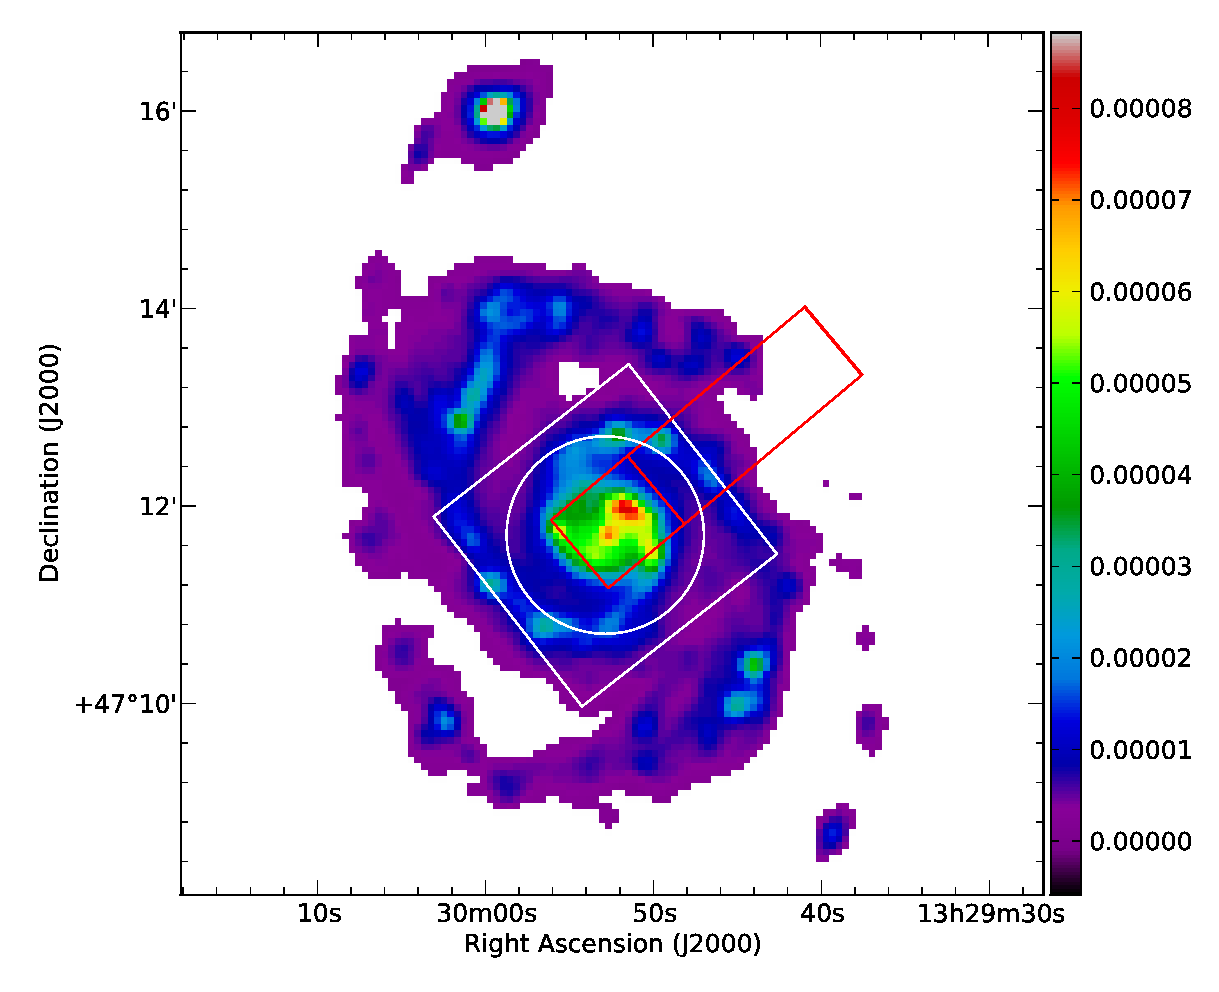
\includegraphics[width=\columnwidth]{ch3/Figure1}
\caption[Total infrared flux of M51]{Total infrared flux, $F_{\mathrm{TIR}}$, calculated using the MIPS~24~$\mu$m and PACS~70~$\mu$m and 160~$\mu$m maps and Equation~(\ref{eqn:Ftir3}).  The map is at the resolution of the PACS 160~$\mu$m map, 12$\arcsec$, and has a plate scale of 4$\arcsec$.  Units are W~m$^{-2}$~sr$^{-1}$.  The white square and red rectangles outline the coverage of the PACS spectroscopic maps and strips, respectively.  The white circle represents the footprint of the SPIRE FTS observations.}
\label{fig:Ltir}
\end{figure}

\subsection{Data Treatment for Analysis}\label{data_treatment}
All of our spectral maps have been convolved with a Gaussian function to a common resolution matching that of the PACS 160~$\mu$m map, 12$\arcsec$.  The MIPS 24~$\mu$m and PACS 70~$\mu$m maps were convolved with the appropriate kernels developed by \citet{2011PASP..123.1218A}.  In addition, each map has been regridded to match the pixel size of the PACS 160~$\mu$m map, 4$\arcsec$.  For the comparison with the PDR models, we applied a 5$\sigma$ cut to our PACS spectroscopic maps to ensure we are considering robust detections in our ratio maps.  Our quoted uncertainties throughout the paper take into account both measurement uncertainties, in calculating the line fluxes for our PACS spectroscopic maps, and calibration uncertainties, unless otherwise noted.  We note here that the calibration uncertainties for the PACS spectroscopy are approximately 30\% and are dominated by small offsets in pointing as well as drifting of the detector response, while the calibration uncertainties for the photometry at 70 and 160~$\mu$m are 3\% and 5\%, respectively (PACS OM).

%%%%%%%%%%%%%%%%%%%%%%%%%%%%%%%%%%%%%%%%%%%%%%%%%%%%%%%%%%%%%%%%%%%%%

\section{Physical characteristics of the gas}\label{gas_char}
\subsection{Line Emission Morphology}\label{morphology}
We present the final maps of the [C\,\textsc{ii}], [N\,\textsc{ii}]122, [O\,\textsc{i}]63, [O\,\textsc{i}]145, [O\,\textsc{iii}], and [N\,\textsc{ii}]205 lines at their native resolution with a 3$\sigma$ cut applied to the PACS maps in Figure~\ref{fig:pacs_spec_maps3}.  We note that the [C\,\textsc{ii}] data were first presented by \citet{2013arXiv1304.1801S} using a different processing method, though it does not play a major role in their analysis. Both the [C\,\textsc{ii}] and [N\,\textsc{ii}]122 maps show similar distributions throughout the center of the galaxy.  Overall there is strong emission in the central $\sim1.\arcmin25$, with the innermost sections of the spiral arms showing the strongest emission.  The average signal to noise ratio (S/N) in the central region is $\sim200$ and 70 for the [C\,\textsc{ii}] and [N\,\textsc{ii}]122 maps, respectively.  The peak in the inner northwestern arm is also present in other wavebands, including, the 24, 70, and 160~$\mu$m images (combined in Figure~\ref{fig:Ltir}), as well as other star formation tracers such as H$\alpha$ and Pa$\alpha$ \citep[e.g.,][]{2003PASP..115..928K,2005ApJ...633..871C}.   The emission is a factor of $\sim$1.5 higher in this peak compared to the center of the galaxy in both [C\,\textsc{ii}] and [N\,\textsc{ii}]122.  The spiral arms can be seen extending outward in weaker emission with a few stronger pockets.

The total [C\,\textsc{ii}] emission in our map is $(2.9 \pm 0.9) \times 10^{-14}$~W~m$^{-2}$ covering an area of $\sim5.5 \times 10^{-7}$~sr$^{-1}$.  \citet{2001ApJ...561..203N} mapped the [C\,\textsc{ii}] emission over a 6$\arcmin \times 6\arcmin$ area of M51 with the KAO and found a peak intensity of $(1.31 \pm 0.15) \times 10^{-4}$~erg~s$^{-1}$~cm$^{-2}$~sr$^{-1}$ in the center of the galaxy.  The integrated intensity of our map over an aperture of approximately 1$\arcmin$ centered on the galaxy (to match the 55$\arcsec$ beam of the KAO) is $\sim (1.4 \pm 0.4) \times 10^{-4}$~erg~s$^{-1}$~cm$^{-2}$~sr$^{-1}$, in good agreement with the KAO measurement.  \citet{2005A&A...441..961K} and \citet{2001A&A...375..566N} both present \emph{ISO} observations of M51 and found a [C\,\textsc{ii}] integrated intensity at the center of $4.41 \times 10^{-5}$~erg~s$^{-1}$~cm$^{-2}$~sr$^{-1}$ and $(9 \pm 2) \times 10^{-5}$~erg~s$^{-1}$~cm$^{-2}$~sr$^{-1}$ within an 80$\arcsec$ beam, respectively, while in an aperture of the same size we measure an integrated intensity of $(1.1 \pm 0.3) \times 10^{-4}$~erg~s$^{-1}$~cm$^{-2}$~sr$^{-1}$.  Our results agree with those of \citet{2001A&A...375..566N} but are higher than those of \citet{2005A&A...441..961K} by about a factor of two.  This discrepancy arises because \citet{2005A&A...441..961K} applied an extended source correction to their observations to obtain the integrated intensity within the \emph{ISO} beam.

The [O\,\textsc{i}]63 map shows a strong spiral arm morphology in the innermost region (average S/N $\sim$40), with a similar peak in the northwest arm to that seen in [C\,\textsc{ii}] and [N\,\textsc{ii}]122.  However, in contrast to the [C\,\textsc{ii}] and [N\,\textsc{ii}]122 emission, the [O\,\textsc{i}]63 emission peaks prominently in the center of the galaxy.  M51 has been classified as a Seyfert~2 \citep{1997ApJS..112..315H}, and thus we believe that the peaked emission in the center may be due to a low-luminosity active nucleus.  We measure a total [O\,\textsc{i}]63 flux within an 80$\arcsec$ beam of $(3 \pm 1) \times 10^{-15}$~W~m$^{-2}$, in good agreement with the values obtained with \emph{ISO} of $(4.4 \pm 0.9) \times 10^{-15}$~W~m$^{-2}$ \citep{2001A&A...375..566N} and $\sim3.9 \times 10^{-15}$~W~m$^{-2}$ \citep{2005A&A...441..961K}.  \citet{2001A&A...375..566N} presented a survey of 34 galaxies, including those classified as AGNs, or Seyfert types.  Comparison of our [O\,\textsc{i}]63 flux obtained for M51 with values from their survey for AGN and Seyfert galaxies shows agreement within a factor of $\sim2$ for most sources, suggesting that our results are typical for galaxies with active centers.

\begin{figure}[!htbp]
 \subfloat[]{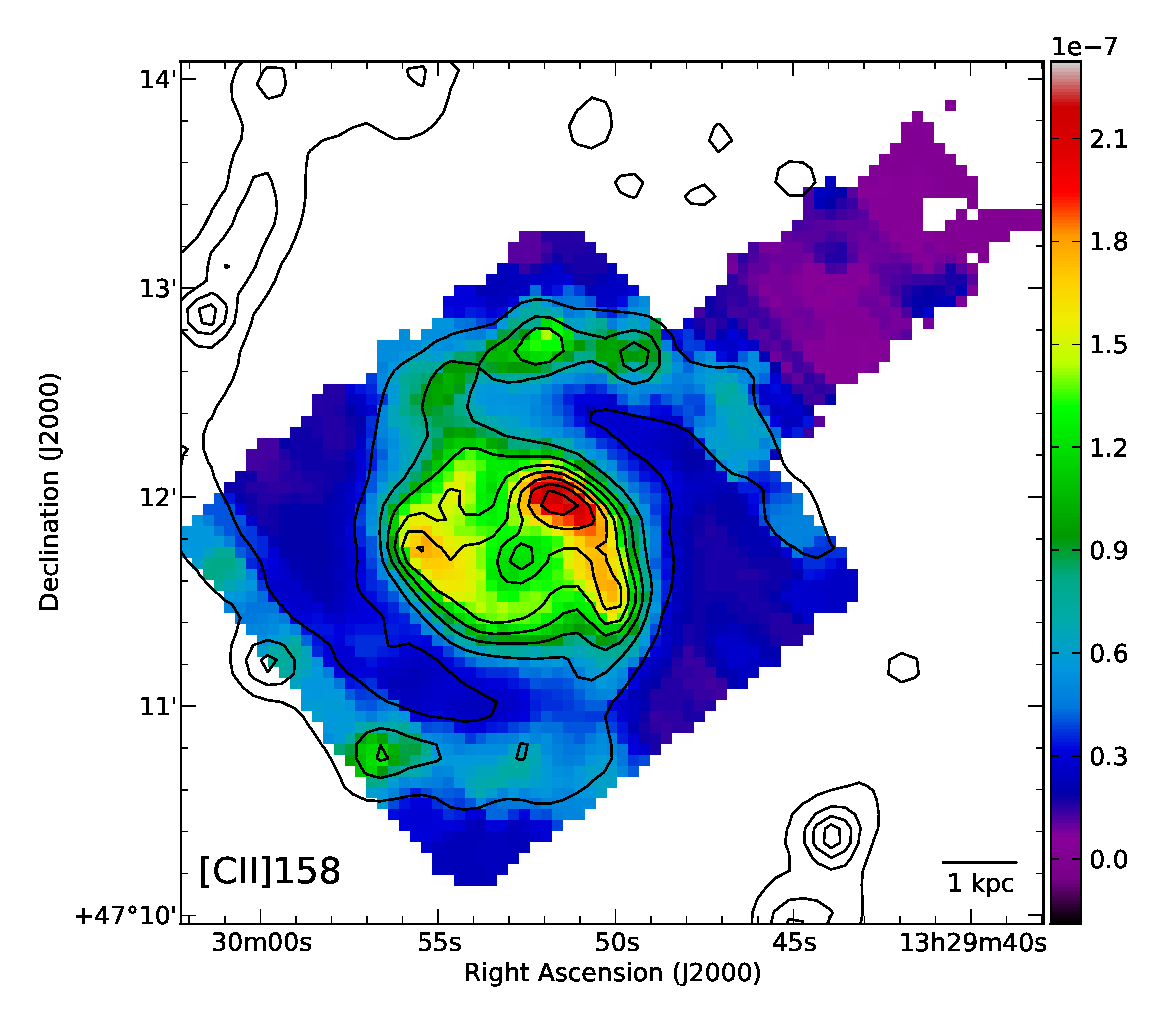
\includegraphics[width=\columnwidth]{ch3/Figure2a}}\\
 \caption[\emph{Herschel} spectroscopic maps of M51 at their native resolution]{\emph{Herschel} PACS and SPIRE spectroscopic maps of M51 of the six fine-structure lines at their native resolution and pixel scale.  We have applied a 3$\sigma$ cutoff to all five PACS images, and the units are W~m$^{-2}$~sr$^{-1}$.  Contours of the total infrared flux are overlaid to direct the eye to the major features of the inner galaxy.  We note that the integrated intensity within each pixel of the [N\,\textsc{ii}]205 map is actually the average surface brightness over the 17$\arcsec$ beam of each bolometer in the FTS array, and not the average over the 4$\arcsec$ pixel each bolometer is centered on.}
\label{fig:pacs_spec_maps3}
\end{figure}
\begin{figure}[!htbp]
\ContinuedFloat
\subfloat[]{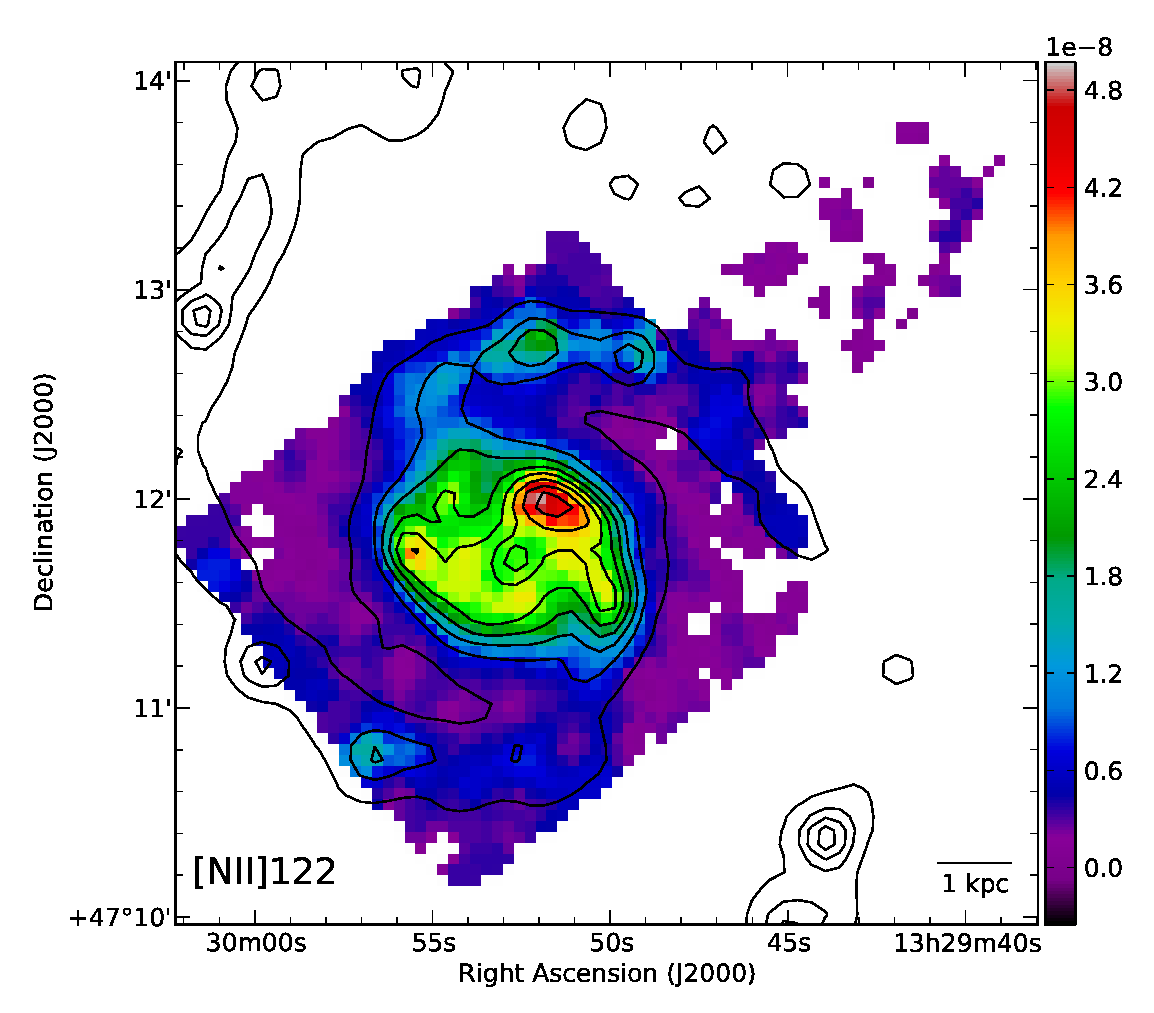
\includegraphics[width=\columnwidth]{ch3/Figure2b}}\\
\caption[]{\emph{continued}}
\end{figure}
\begin{figure}[!htbp]
\ContinuedFloat
 \subfloat[]{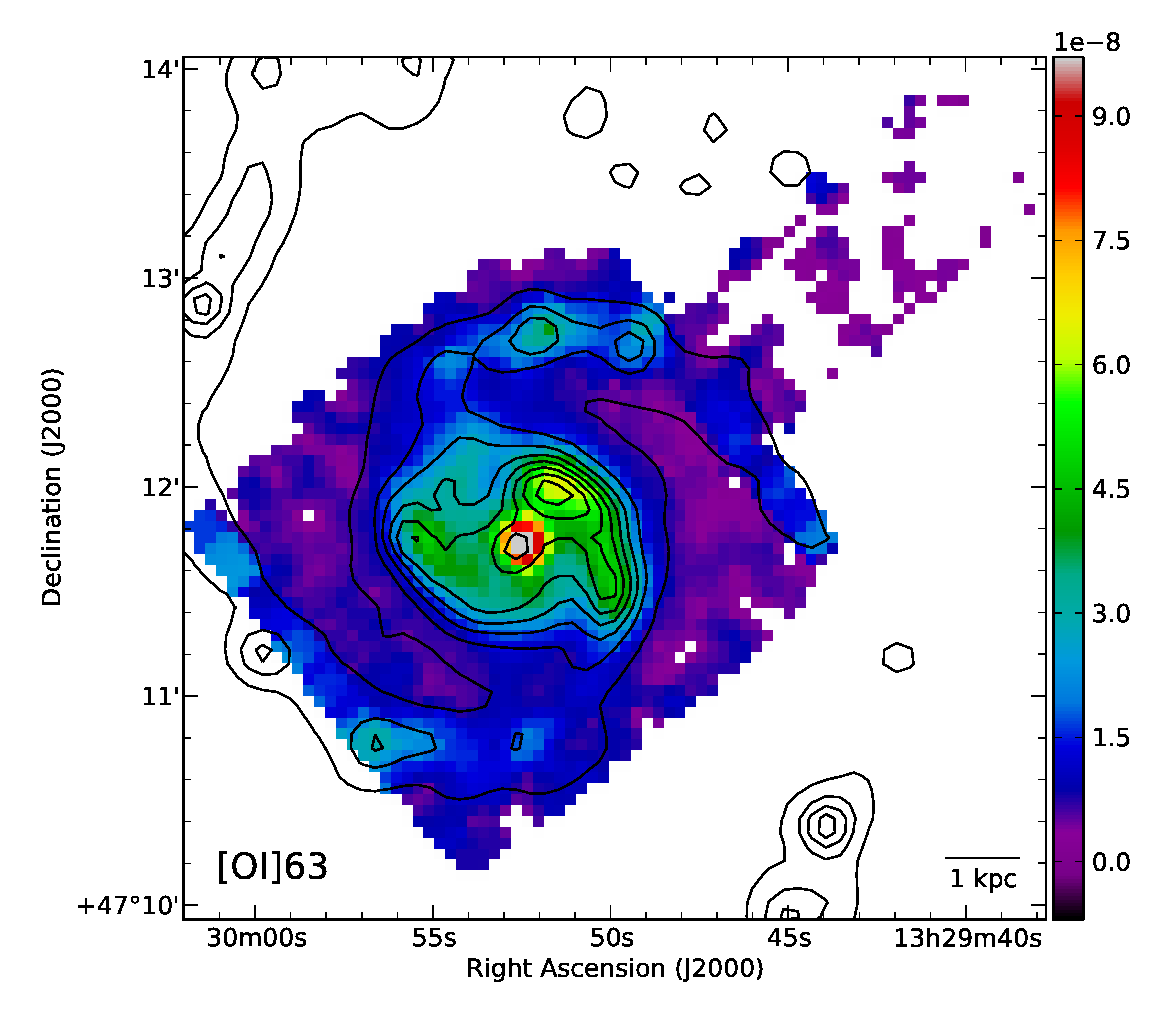
\includegraphics[width=\columnwidth]{ch3/Figure2c}}\\
 \caption[]{\emph{continued}}
\end{figure}
\begin{figure}[!htbp]
\ContinuedFloat
 \subfloat[]{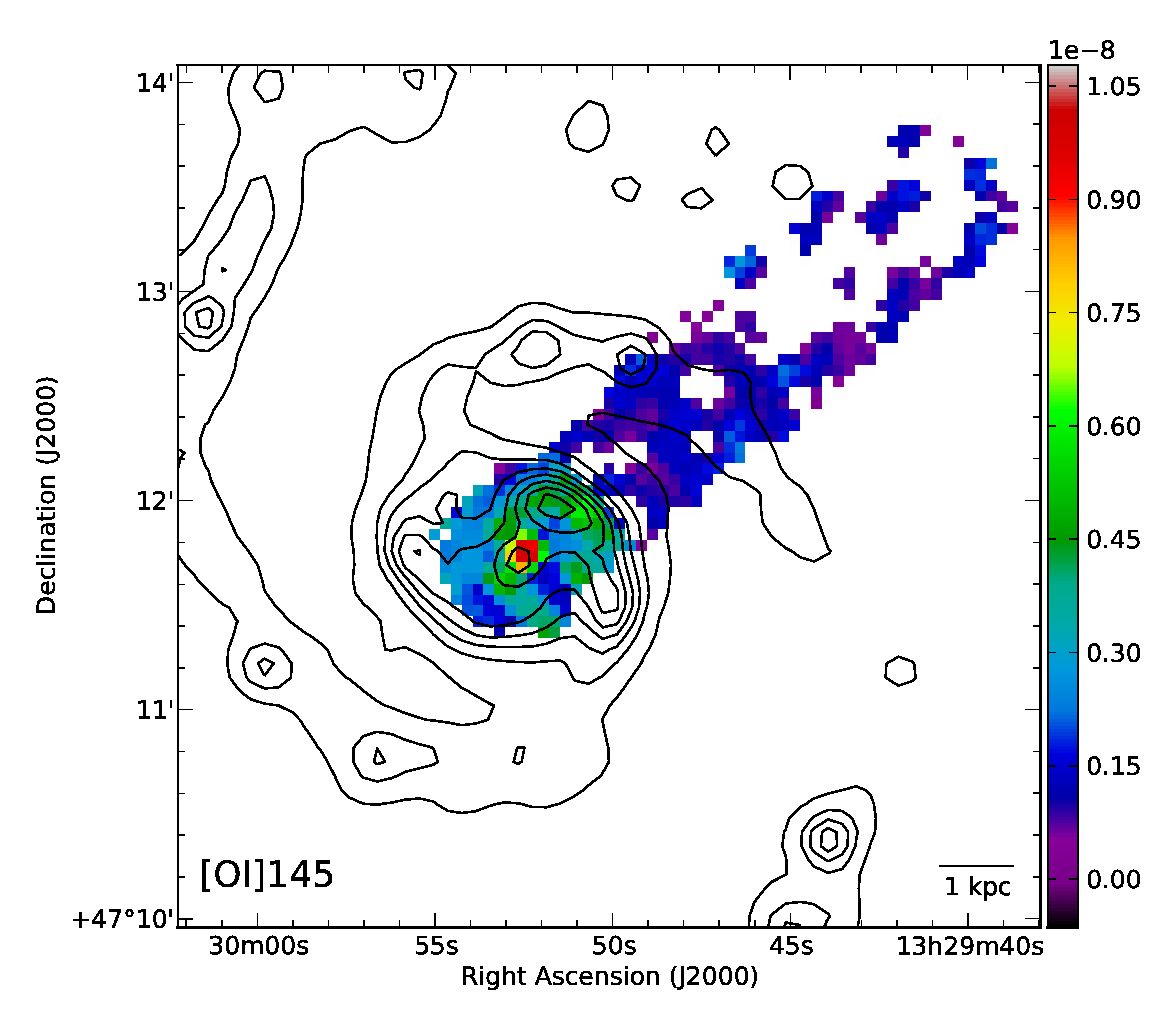
\includegraphics[width=\columnwidth]{ch3/Figure2d}}\\
 \caption[]{\emph{continued}}
\end{figure}
\begin{figure}[!htbp]
 \ContinuedFloat
 \subfloat[]{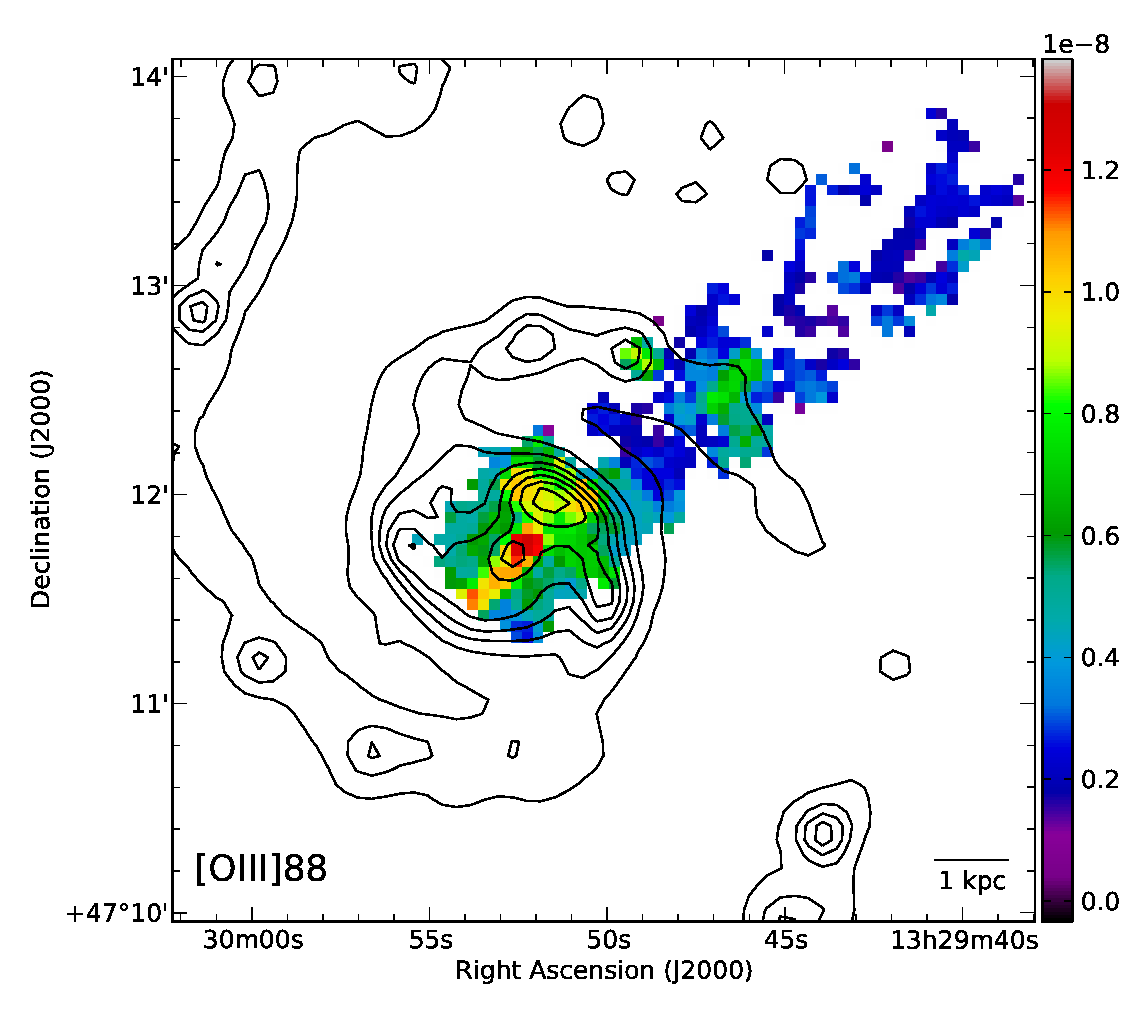
\includegraphics[width=\columnwidth]{ch3/Figure2e}}\\
 \caption[]{\emph{continued}}
\end{figure}
\begin{figure}[!htbp]
 \ContinuedFloat
 \subfloat[]{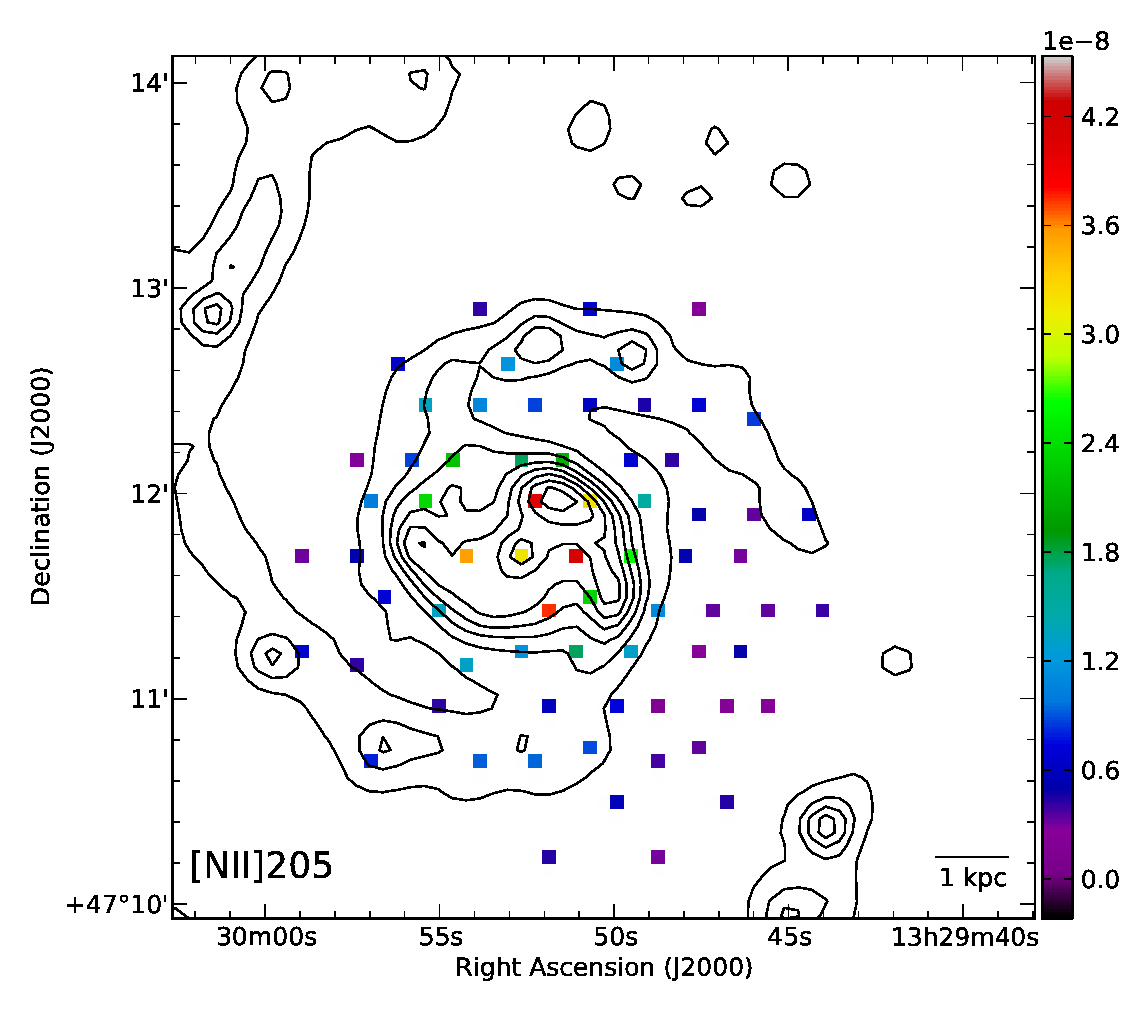
\includegraphics[width=\columnwidth]{ch3/Figure2f}}\\
 \caption[]{\emph{continued}}
\end{figure}

As we have only observed M51 along a strip in [O\,\textsc{i}]145 and [O\,\textsc{iii}] emission, the maps cover much less area.  [O\,\textsc{iii}] emission is concentrated primarily in the nuclear region with a peak in the very center and a slight enhancement in the northwestern inner region of the spiral arm.  There is also a ``stripe'' extending from the center to the southeast that may indicate a bar-like structure.  Overall, the flux in this line is weaker than in [C\,\textsc{ii}], [N\,\textsc{ii}]122, and [O\,\textsc{i}]63 emission, in part due to the fact that the line is intrinsically weak.  However, there is also less sensitivity in the strips than the maps due to the raster spacing in the strips.  The average S/N in the central part of the [C\,\textsc{ii}] map is $\sim$200, while it is only about 8 and 11 for the central footprint in the [O\,\textsc{iii}] and [O\,\textsc{i}]145 strips, respectively.  The morphology of the center of the [O\,\textsc{i}]145 strip looks very similar to the [O\,\textsc{i}]63 emission, only weaker.  We note here that \citet{2001A&A...375..566N} observed the [O\,\textsc{i}]145 line with \emph{ISO} but did not detect it, while they measured a flux of $(0.8 \pm 0.3) \times 10^{-15}$~W~m$^{-2}$ for the [O\,\textsc{iii}] line, twice as high as our measured value of $(3 \pm 1) \times 10^{-16}$~W~m$^{-2}$.  This is likely because we only observed a strip in this line and thus the 80$\arcsec$ aperture of \citet{2001A&A...375..566N} is larger than our observed region.

In Table~\ref{table:total_flux} we compare the total flux of each line with previous work.  In a region approximately $2.\arcmin7$ from the center of M51, centered on the H\textsc{ii} region CCM~10, \citet{2004AJ....128.2772G} used \emph{ISO} to observe the same fine-structure lines as we present here.  \citet{2005A&A...441..961K} also observed M51 with \emph{ISO} in the center and two locations in the spiral arms, detecting [C\,\textsc{ii}], [O\,\textsc{i}]63, and [N\,\textsc{ii}]122, while \citet{2001A&A...375..566N} presented observations of the center taken with \emph{ISO} and detected the same lines we have, with the exception of the [O\,\textsc{i}]145 line.  To compare our results to these previous observations, we have calculated the flux within the central 80$\arcsec$ for each line to match the beam size of a single pointing with \emph{ISO}.  In general our measurements agree well with those of \citet{2001A&A...375..566N}; however, our values are stronger than those of \citet{2004AJ....128.2772G}.  This is a reasonable result given that CCM~10 is located in a region outside the central 80$\arcsec$ aperture and in fact falls outside our observed region entirely.

\begin{landscape}
\begin{deluxetable}{lcccc}
\tabletypesize{\small}
\tablecolumns{5}
\tablecaption{Comparison to Previous Measurements of M51\label{table:total_flux}}
\tablewidth{0pt}
\tablehead{
\colhead{Line} & \multicolumn{4}{c}{Flux ($10^{-16}$~W~m$^{-2}$)} \\
\colhead{}     & \colhead{This Work} & \colhead{\citet{2004AJ....128.2772G}}
		& \colhead{\citet{2001A&A...375..566N}} & \colhead{\citet{2005A&A...441..961K}} \\
\colhead{}	   & \colhead{Central 80$\arcsec$\tablenotemark{a}} & \colhead{CCM~10\tablenotemark{b}}
		       & \colhead{Center} & \colhead{Center\tablenotemark{c}}}
 \startdata
 $[$C\,\textsc{ii}$]$(158~$\mu$m) & $135 \pm 40$  & $39 \pm 3$    & $104 \pm 21$ & $52.92$ \\
 $[$N\,\textsc{ii}$]$(122~$\mu$m) & $24 \pm 7$    & $3.3 \pm 0.1$ & $21 \pm 4$   & 14.76   \\
 $[$O\,\textsc{i}$]$(63~$\mu$m)   & $30 \pm 10$   & $14 \pm 4$    & $44 \pm 9$   & 38.64   \\
 $[$O\,\textsc{i}$]$(145~$\mu$m)  & $1.5 \pm 0.4$ & $0.8 \pm 0.2$ & \nodata      & \nodata \\
 $[$O\,\textsc{iii}$]$(88~$\mu$m) & $3 \pm 1$     & $8 \pm 2$     & $8 \pm 3$    & \nodata \\
 \enddata
 \tablecomments{Total flux measured within an 80$\arcsec$ aperture centered on the nucleus of M51.  The aperture matches the beam size of the \emph{ISO} observations.  Only pixels with a 5$\sigma$ detection or better within the aperture were included in calculating the total flux from our \emph{Herschel} maps.}
 \tablenotetext{a}{The number of pixels with at least a 5$\sigma$ detection within the 80$\arcsec$ aperture varies between lines.  The [C\,\textsc{ii}], [N\,\textsc{ii}], and [O\,\textsc{i}]63 lines are detected in all pixels within the aperture, covering a total solid angle of $1.2 \times 10^{-7}$~sr.  The solid angle covered by the [O\,\textsc{i}]145 emission within the aperture is $4.6 \times 10^{-8}$~sr, and the solid angle covered by the [O\,\textsc{iii}] emission within the aperture is $4.9 \times 10^{-8}$~sr.}
 \tablenotetext{b}{CCM~10 is an H\,\textsc{ii} region that lies outside the region discussed in this work.}
 \tablenotetext{c}{These are the same data as presented by \citet{2001A&A...375..566N}; however, an extended source correction has been applied by \citet{2005A&A...441..961K} in calculating the integrated intensity, reducing its value.}
\end{deluxetable}
\end{landscape}

\subsection{Line Deficits}\label{ratio3}
In Figure~\ref{fig:ratio_plots}(a) we show the [C\,\textsc{ii}]/$F_{\mathrm{TIR}}$ ratio, which varies between $10 \times 10^{-4}$ and $100 \times 10^{-4}$ with an average $40 \times 10^{-4}$.  Typical measurement uncertainties (excluding calibration errors) in a given pixel are $\sim 3$\%, with the highest measurement uncertainties (and thus lowest S/N) of $\sim 20$\% found in the pixels on the outermost edges of the map. There are a few regions along the spiral arms in the north and southwest of the map where there is a small enhancement of the ratio, corresponding to peaks in the [C\,\textsc{ii}] emission.  In addition, we see a lower ratio in the center of the galaxy, corresponding to a slight deficit of [C\,\textsc{ii}] emission.  The average [C\,\textsc{ii}]/$F_{\mathrm{TIR}}$ ratio, along with the line/$F_{\mathrm{TIR}}$ ratio for each of the other far-infrared lines, is shown in Table~\ref{tbl:line2tir}.  Not surprisingly, the next strongest ratio after the [C\,\textsc{ii}]/$F_{\mathrm{TIR}}$ ratio is the [O\,\textsc{ii}]63/$F_{\mathrm{TIR}}$ ratio.  The emission from these lines accounts for between 0.01\% and 0.4\% of the total infrared flux in this region of M51.

\begin{deluxetable}{lcc}
\tabletypesize{\small}
\tablecolumns{3}
\tablecaption{Line to Total Infrared Flux Ratio in M51\label{tbl:line2tir}}
\tablewidth{0pt}
\tablehead{
\colhead{Line} 	            & \colhead{$10^{-4}$ Line/$F_{\mathrm{TIR}}$\tablenotemark{a}} &
	\colhead{Area\tablenotemark{b} ($\sq\arcsec$)}}
  \startdata
 $[$C\,\textsc{ii}](158~$\mu$m) & $40 \pm 10$ & 21360 \\
 $[$N\,\textsc{ii}](122~$\mu$m) & $5 \pm 1$ & 17536 \\
 $[$O\,\textsc{i}](63~$\mu$m)   & $9 \pm 3$ & 17472 \\
 $[$O\,\textsc{i}](145~$\mu$m)  & $1.0 \pm 0.7$ & 3008 \\
 $[$O\,\textsc{iii}](88~$\mu$m) & $2 \pm 1$ & 2976 \\
 \enddata
 \tablenotetext{a}{Average spectral line flux divided by the total infrared flux, as calculated using our 5$\sigma$-cut maps for M51.  The uncertainties shown are the standard deviations.}
 \tablenotetext{b}{The area over which each average is calculated.  The variations reflect the size differences in our maps between different fine-structure lines.}
\end{deluxetable}

\begin{figure}[!htbp]
\subfloat[]{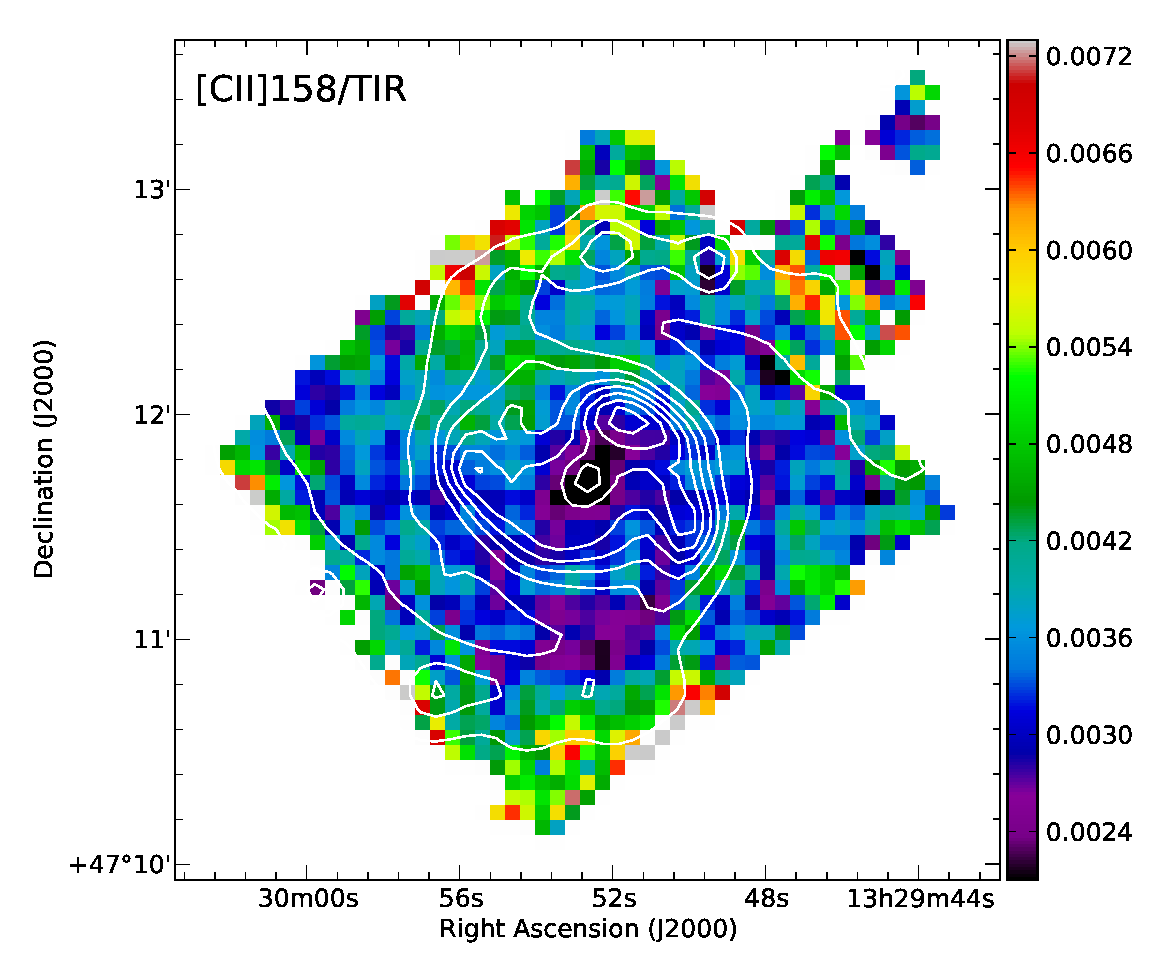
\includegraphics[width=\columnwidth]{ch3/Figure3a}}\\
\caption[Maps of important line ratios in M51]{(a) The [C\,\textsc{ii}] emission divided by the total infrared flux, $F_{\mathrm{TIR}}$, in M51.  (b) The sum of the [C\,\textsc{ii}] and [O\,\textsc{i}]63 emission in M51 divided by the total infrared flux, $F_{\mathrm{TIR}}$.  (c) The [C\,\textsc{ii}] emission in M51 divided by the [O\,\textsc{i}]63 emission.  A 5$\sigma$ cutoff has been applied to all of the spectral line maps.  Contours of $F_{\mathrm{TIR}}$ are overlaid on each ratio plot to highlight the major features of the galaxy.}
\label{fig:ratio_plots}
\end{figure}
\begin{figure}[!htbp]
\ContinuedFloat
\subfloat[]{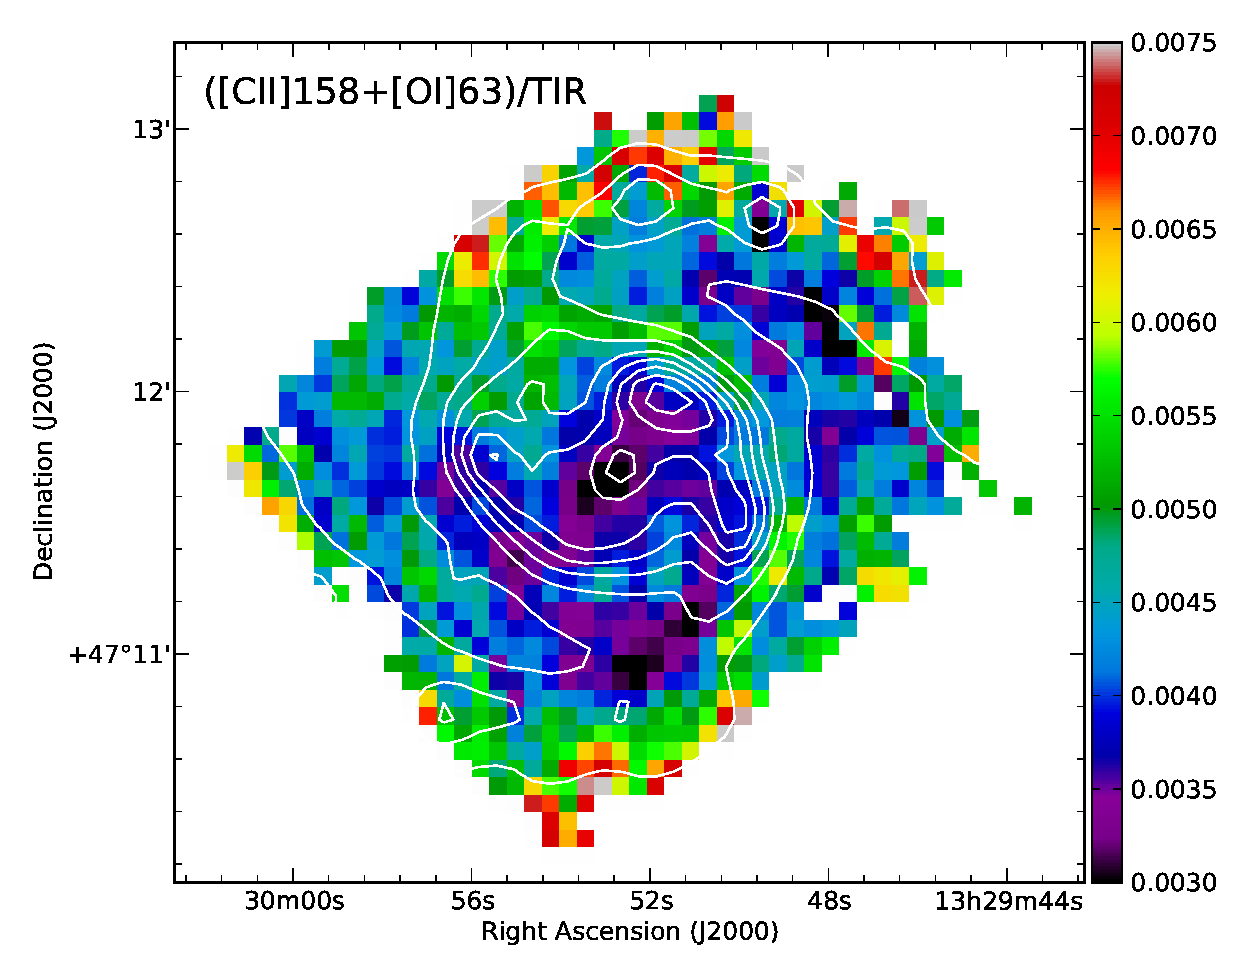
\includegraphics[width=\columnwidth]{ch3/Figure3b}}\\
\caption[]{\emph{continued}}
\end{figure}
\begin{figure}[!htbp]
\ContinuedFloat
\subfloat[]{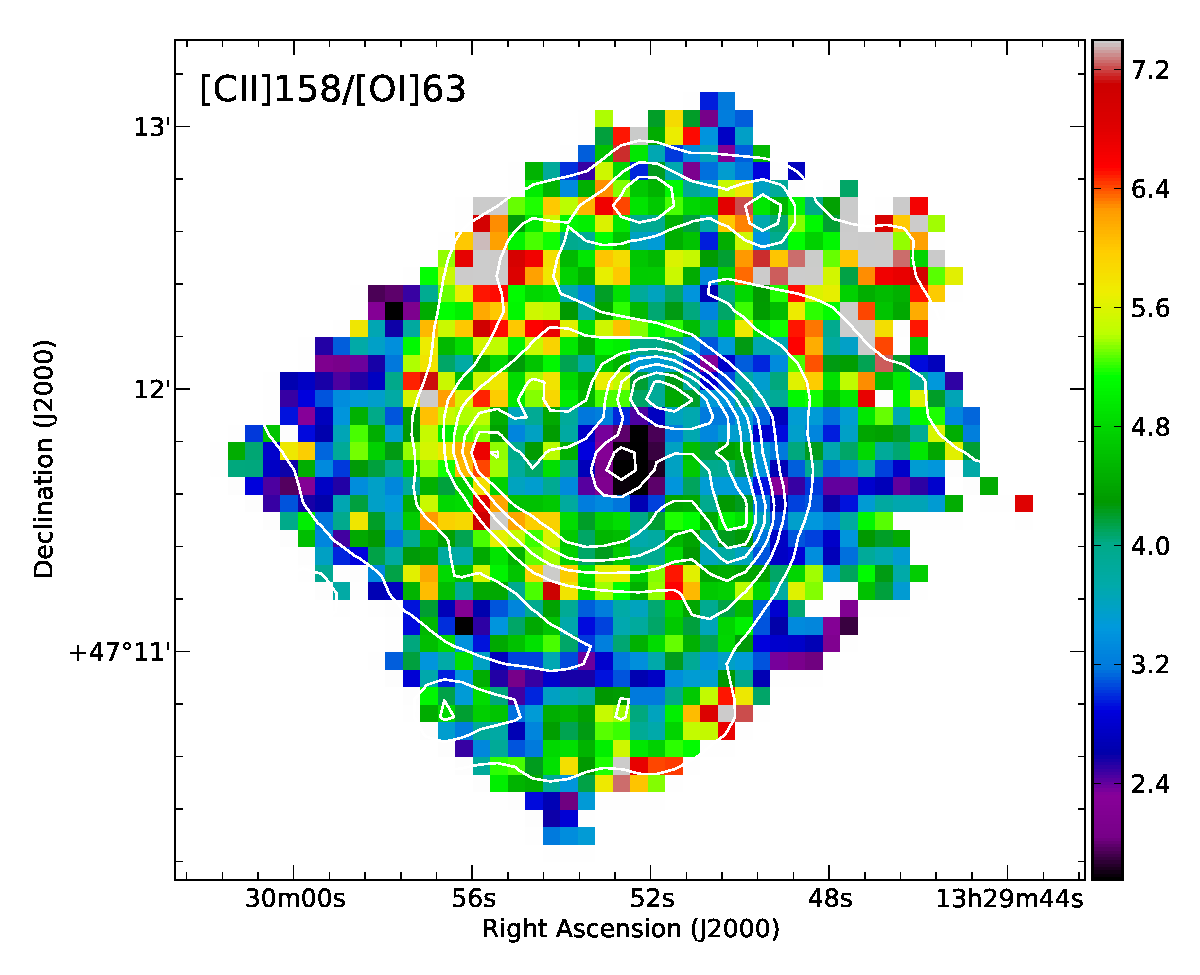
\includegraphics[width=\columnwidth]{ch3/Figure3c}}\\
\caption[]{\emph{continued}}
\end{figure}

The global [C\,\textsc{ii}]/$F_{\mathrm{TIR}}$ ratio has been measured by numerous surveys of both nearby galaxies and high-redshift sources to investigate the [C\,\textsc{ii}] deficit.  Studies of the [C\,\textsc{ii}]/$L_{\mathrm{FIR}}$ ratio in ultra-luminous infrared galaxies (ULIRGs) show a deficit when compared to normal galaxies, with values of less than $5 \times 10^{-4}$ \citep[e.g.,][]{1998ApJ...504L..11L,2003ApJ...594..758L}.  This is the so-called [C\,\textsc{ii}] deficit.  Multiplying our [C\,\textsc{ii}]/$F_{\mathrm{TIR}}$ ratio by a factor of 1.3 to convert $F_{\mathrm{TIR}}$ to $F_{\mathrm{FIR}}$ \citep{2008A&A...479..703G}, we find that our [C\,\textsc{ii}]/$F_{\mathrm{FIR}}$ range of $13 \times 10^{-4}$ to $130 \times 10^{-4}$ with an average $52 \times 10^{-4}$ is in good agreement with previous studies of the [C\,\textsc{ii}]/$F_{\mathrm{FIR}}$ ratio.  \citet{2001ApJ...561..203N} previously investigated M51 and found that this ratio varied between $60 \times 10^{-4}$ and $140 \times 10^{-4}$.  \citet{1985ApJ...289..803S} found a global value for the [C\,\textsc{ii}]/$F_{\mathrm{FIR}}$ ratio within the Milky Way of $30 \times 10^{-4}$ and on smaller scales, \citet{1993ApJ...404..219S} found the same value for the Orion molecular cloud.  \citet{1985ApJ...291..755C} conducted a study of six gas-rich galaxies, including M51, and found that the ratio is about $50 \times 10^{-4}$ for this sample. \citet{2001ApJ...561..766M} found ratios of greater than $20 \times 10^{-4}$ in two-thirds of their sample of 60 normal star-forming galaxies, and \citet{2011ApJ...728L...7G} found a range of values between $1 \times 10^{-4}$ and $100 \times 10^{-4}$ for a sample of 44 AGN and starburst-type galaxies from the SHINING survey.  On smaller scales, \citet{2002AJ....124..751C} investigated NGC~6946 and NGC~1313 and found that the ratio for these two galaxies is $80 \times 10^{-4}$, while \citet{2013A&A...549A.118C} found that the [C\,\textsc{ii}]/$F_{\mathrm{FIR}}$ ratio varies between roughly $10 \times 10^{-4}$ and $100 \times 10^{-4}$ for various regions within the starburst M82.  \citet{2013A&A...553A.114K} recently discovered a radial trend in the [C\,\textsc{ii}]/$F_{\mathrm{FIR}}$ ratio in M33, increasing from $80 \times 10^{-4}$ in the inner galaxy to $300 \times 10^{-4}$ at a distance of roughly 4.5~kpc from the center, and thus increasing with decreasing far-infrared flux.

We also compare our results to the empirically derived relation from \citet{2012ApJ...745..171S} predicting the global [C\,\textsc{ii}] luminosity given a galaxy's total infrared luminosity.  Using our total-infrared luminosity of $4.71 \times 10^{10} L_{\odot}$ and Equation~(33) from \citet{2012ApJ...745..171S}, we calculate a global [C\,\textsc{ii}] luminosity of $7.5 \times 10^{7} L_{\odot}$ and thus a [C\,\textsc{ii}]/$L_{\mathrm{FIR}}$ ratio of $16 \times 10^{-4}$.  This value is in agreement with the lower range of our observed values.  Thus, we find that even though our [C\,\textsc{ii}]/$F_{\mathrm{FIR}}$ ratio is smaller (by up to a factor of two) in the nucleus than in the rest of M51, it is not as extreme as the low values seen in ULIRGs.

\citet{2001A&A...375..566N} calculated the line/$F_{\mathrm{TIR}}$ ratio for the same far-infared lines we measured here with PACS.  Their sample of galaxies, including normal, starburst, and AGN types, shows line/$F_{\mathrm{TIR}}$ ratios consistent with those measured in M51.  Furthermore, our results for M51 are also consistent with the results \citet{2001ApJ...561..766M} found for their sample of normal galaxies (note we have increased their far-infrared flux values by a factor of 1.3 to approximate the total infrared flux).  We compare our results to both papers in Table~\ref{tbl:comp_line2tir}.  Our resolved average values for M51 fall within the range of ratios typically found in a variety of galaxy types on unresolved scales.

\begin{deluxetable}{lcccc}
\tabletypesize{\small}
\tablecolumns{5}
\tablecaption{Line/$F_{\mathrm{TIR}}$ Ratios in M51 Compared to Previous Global Surveys\label{tbl:comp_line2tir}}
\tablewidth{0pt}
\tablehead{
\colhead{Line}	            & \multicolumn{4}{c}{$10^{-4}$ Line/$F_{\mathrm{TIR}}$} \\
\colhead{} & \multicolumn{2}{c}{This Work\tablenotemark{a}} & \colhead{\citet{2001A&A...375..566N}} & \colhead{\citet{2001ApJ...561..766M}} \\
\colhead{} & \colhead{Average} & \colhead{Range} & \colhead{} & \colhead{}}
  \startdata
 $[$C\,\textsc{ii}](158~$\mu$m) & $40 \pm 10$   & 9--100 & 7--50  & 2--100 \\
 $[$N\,\textsc{ii}](122~$\mu$m) & $5 \pm 1$     & 2--10 & 1--7   & 0.8--8 \\
 $[$O\,\textsc{i}](63~$\mu$m)   & $9 \pm 3$     & 4--30 & 4--40  & 5--30 \\
 $[$O\,\textsc{i}](145~$\mu$m)  & $1.0 \pm 0.7$ & 0.3--5 & \nodata & \nodata \\
 $[$O\,\textsc{iii}](88~$\mu$m) & $2 \pm 1$     & 0.9--8 & 1--10  & 2--20 \\
 \enddata
 \tablenotetext{a}{Note that only 5$\sigma$ detections are included; global values for M51 are likely to be lower.}
\end{deluxetable}

\subsection{Heating and Cooling}
In Figure~\ref{fig:ratio_plots}(b) we show a map of ([C\,\textsc{ii}]+[O\,\textsc{i}]63)/$F_{\mathrm{TIR}}$, which is considered a proxy for the total heating efficiency, $\epsilon$ \citep{1985ApJ...291..722T}.  The heating efficiency represents the fraction of energy from the interstellar FUV radiation field that is converted to gas heating through the photoelectric effect, divided by the fraction of its energy deposited in dust grains.  This ratio represents the heating efficiency within the context of gas heating in PDR regimes \citep[see, e.g.,][]{1985ApJ...291..722T}.  A comparison with the [C\,\textsc{ii}]/$F_{\mathrm{TIR}}$ ratio shows that adding the [O\,\textsc{i}]63 emission enhances some of the structure in the spiral arms.  We look at this ratio in more detail in Section~\ref{pdr_model3}.

The [C\,\textsc{ii}]/[O\,\textsc{i}]63 ratio is also shown in Figure~\ref{fig:ratio_plots}(c).  Cooling via the [C\,\textsc{ii}] line is more efficient in lower density, lower temperature regimes, while [O\,\textsc{i}]63 cooling dominates at higher densities and warmer temperatures \citep{1985ApJ...291..722T}.  In this figure, the central region shows a ratio lower than the rest of the galaxy by a factor of $\sim$2--4, corresponding to the strong [O\,\textsc{i}]63 emission in the center; however, the ratio remains greater than 1.0 everywhere.  There is a visible increase in the ratio to upward of 6.0 along the inner part of the eastern spiral arm, spatially coincident with the decreasing [C\,\textsc{ii}] emission at the outer edge of the nuclear region.  The low ratio in the center of the galaxy might indicate that the gas is warmer and/or more dense, and cooling by the [O\,\textsc{i}]63 line becomes more important.  Typical measurement uncertainties are about 8\% with the noisiest pixels lying around the edge of the map having uncertainties of up to $\sim 24$\%.

The ratio of the two [O\,\textsc{i}] lines, [O\,\textsc{i}]145/[O\,\textsc{i}]63, can probe the temperature in the range around $\sim 300$~K for optically thin neutral gas because the excitation energies, $\Delta E/k$, are 228~K and 325~K above the ground state for the [O\,\textsc{i}]63 and [O\,\textsc{i}]145 lines, respectively \citep{1985ApJ...291..722T, 1999ApJ...527..795K, 2001ApJ...561..766M, 2006A&A...446..561L}.  However, the [O\,\textsc{i}]63 line can become optically thick at a lower column density than the [O\,\textsc{i}]145 line, boosting the ratio of the two [O\,\textsc{i}] lines for gas temperatures less than $\sim 1000$~K \citep{1985ApJ...291..722T}.  Using a 5$\sigma$ cutoff for both the [O\,\textsc{i}]63 and [O\,\textsc{i}]145 lines and noting that the [O\,\textsc{i}]145 was only mapped along a radial strip (see Figure~\ref{fig:pacs_spec_maps3}), our measurements of the ratio reside primarily in the central region of the galaxy, along with a few pixels in the inner part of the northwestern spiral arm.  In the center region the average ratio is 0.08 with typical measurement uncertainties of $\sim 9$\%.  Taking the inverse of this value to obtain a [O\,\textsc{i}]63/[O\,\textsc{i}]145 ratio of $12.5 \pm 5.3$ and comparing it with Figure~4 from \citet{2006A&A...446..561L}, we find that the [O\,\textsc{i}]63 line is either optically thick with $T \gtrsim 200$~K and $n \gtrsim 10^{3}$~cm$^{-3}$ or optically thin and hot with $T \sim 4000$~K and a density of approximately $10^{3}$~cm$^{-3}$.

We can also investigate the diagnostic plots ([C\,\textsc{ii}]+[O\,\textsc{i}]63)/$F_{\mathrm{TIR}}$ or ([C\,\textsc{ii}] + [O\,\textsc{i}]63)/$F_{\mathrm{PAH}}$ versus far-infrared color to look at the heating efficiency in more depth. Here we take the far-infared color 70$\mu$m/160$\mu$m, but typically the \emph{IRAS} color 60$\mu$m/100$\mu$m is used.  Previous work has found a correlation between the heating efficiency and the infared color showing a decrease in heating efficiency with warmer colors, on both global and galactic scales \citep[e.g.,][]{2001ApJ...561..766M,2012ApJ...747...81C}. This decrease has been attributed to warmer dust grains becoming increasingly positively charged when exposed to stronger radiation fields, thus lowering the efficiency of the photoelectric effect.  It has also been shown that there is an even tighter correlation between heating efficiency and PAH emission, perhaps indicating that PAHs are the primary contributor to gas heating rather than dust grains in regions where [C\,\textsc{ii}] and [O\,\textsc{i}]63 are the primary coolants \citep{2012ApJ...747...81C, 2012A&A...548A..91L}.  In Figure~\ref{fig:heating_efficiency} we plot ([C\,\textsc{ii}]+[O\,\textsc{i}]63)/$F_{\mathrm{TIR}}$ as a function of 70$\mu$m/160$\mu$m (top) and ([C\,\textsc{ii}]+[O\,\textsc{i}]63)/$F_{\mathrm{PAH}}$ as a function of color (bottom).  In both cases, each data point corresponds to one pixel in our images and the colors correspond to the four different regions we break the galaxy into for our PDR analysis (see Section~\ref{pdr_model3} and Figure~\ref{fig:regions} for more details).  We find that the heating efficiency as traced by ([C\,\textsc{ii}]+[O\,\textsc{i}]63)/$F_{\mathrm{TIR}}$ decreases by about a factor of two with increasing color as found by previous studies, which corresponds to a lower heating efficiency in the center of the galaxy than in the arm and interarm regions.  When we trace the heating efficiency by ([C\,\textsc{ii}]+[O\,\textsc{i}]63)/$F_{\mathrm{PAH}}$, we find a variation of approximately 30\% across the color space, in agreement with general trends found by \citet{2012A&A...548A..91L} in LMC~N11B and \citet{2012ApJ...747...81C} in NGC~1097 and NGC~4559.  However, this ratio does not vary significantly for the warmer dust, in contrast to the ([C\,\textsc{ii}]+[O\,\textsc{i}]63)/$F_{\mathrm{TIR}}$ ratio.

\begin{figure}
\centering
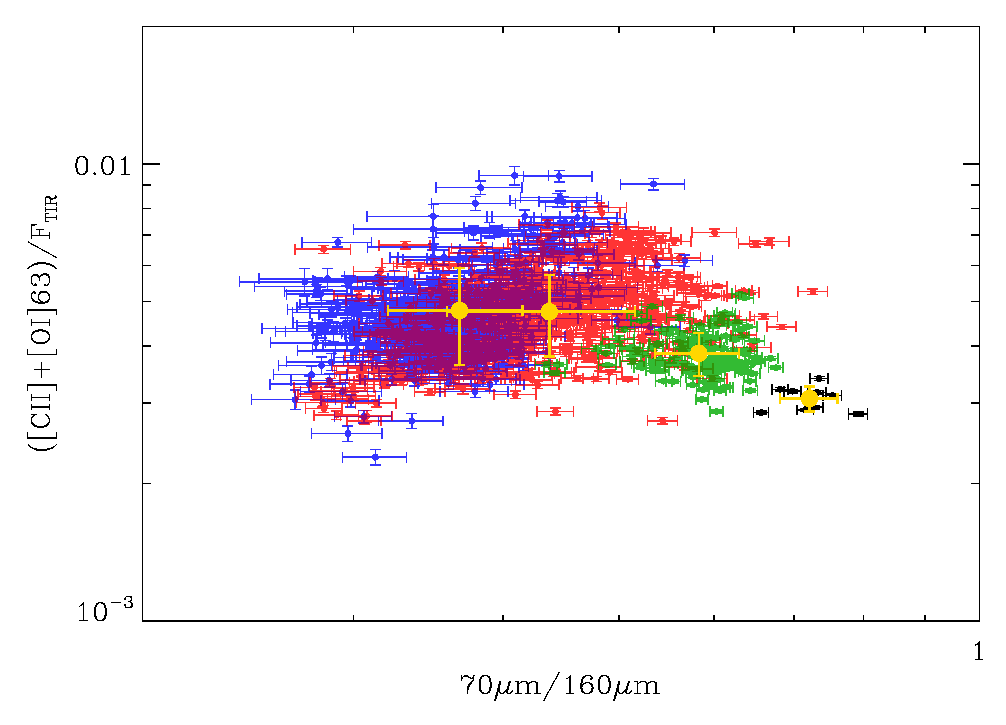
\includegraphics[width=0.9\columnwidth]{ch3/Figure4a}
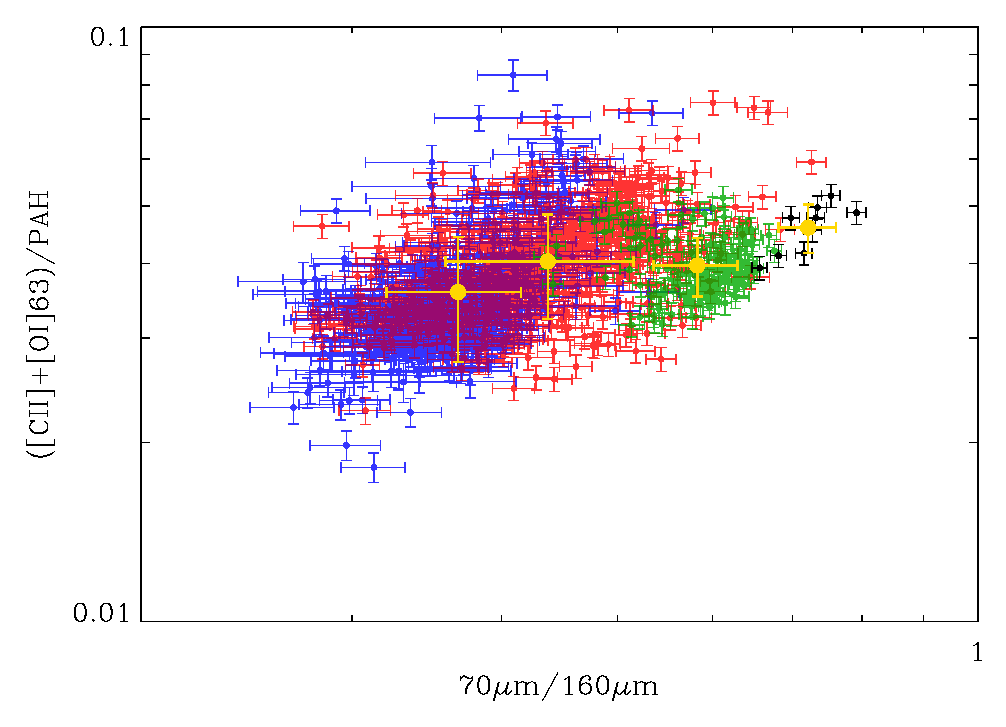
\includegraphics[width=0.9\columnwidth]{ch3/Figure4b}
\caption[Heating efficiency as a function of the 70$\mu$m/160$\mu$m color in M51]{Top: total cooling ([C\,\textsc{ii}]+[O\,\textsc{i}]63) divided by the total infrared flux vs. the PACS 70$\mu$m/160$\mu$m color.  Bottom: total cooling ([C\,\textsc{ii}]+[O\,\textsc{i}]63) divided by the PAH emission, represented by the stellar subtracted IRAC 8~$\mu$m flux, vs. the PACS 70$\mu$m/160$\mu$m color.  In both cases, one data point represents one pixel.  The pixels from the nucleus, center, arm, and interarm regions are shown in black, green, red and blue, respectively.  The large yellow circles represent the mean for each region.}
\label{fig:heating_efficiency}
\end{figure}

Our value for the total heating efficiency within PDRs as measured by ([C\,\textsc{ii}] + [O\,\textsc{i}]63)/$F_{\mathrm{TIR}}$ ranges between approximately $2 \times 10^{-3}$ and $5 \times 10^{-3}$.  The survey conducted by \citet{2001ApJ...561..766M} found a range of values between $10^{-3}$ and $10^{-2}$.  \citet{2012ApJ...747...81C} looked at NGC~1097 and NGC~4559 and found that this proxy for the heating efficiency falls between approximately $2 \times 10^{-3}$ to $10^{-2}$; thus, our values for M51 fall within the lower range of their results.  In slightly lower metallicity environments the ratio is about the same at $2.77 \times 10^{-3}$ for NGC~4214 \citep[metallicity of log(O/H)$+ 12 = 8.2$;][]{2010A&A...518L..57C} and $2 \times 10^{-3}$ in Haro~11 \citep[metallicity 1/3 solar;][]{2012A&A...548A..20C}.  On small scales, \citet{2012A&A...548A..91L} investigated the H\,\textsc{ii} region LMC-N11B (metallicity $\sim$1/2 solar), and found an average value of $\sim 5.5 \times 10^{-3}$ in PDRs, but the ratio decreased in regions dominated by ionized gas, a trend they attribute to contamination of the total infrared flux from the ionized gas where [C\,\textsc{ii}] and [O\,\textsc{i}]63 do not primarily emit.

Looking at the ([C\,\textsc{ii}]+[O\,\textsc{i}]63)/PAH ratio, we find an average of $\sim0.01$, which is less than the value of 0.07 in LMC-N11B \citep{2012A&A...548A..91L}, as well as the range of 0.035--0.06 in NGC~1097 and NGC~4559 \citep{2012ApJ...747...81C}.  \citet{2012ApJ...751..144B} find that the ([C\,\textsc{ii}]+[O\,\textsc{i}]63)/PAH ratio varies from 0.03 to 0.1 and is approximately 50\% lower in the ring of NGC~1097 than in the nucleus.  However, \citet{2012ApJ...747...81C} note that for NGC~1097 and NGC~4559, using the IRAC 8$\mu$m map as a proxy for the total PAH emission overestimates (by about 10\%) the true total emission, estimated from running the \emph{Spitzer} Infrared Spectrograph (IRS) spectrum through PAHfit \citep{2007ApJ...656..770S}.  As a similar check for M51, we run the IRS spectrum for M51 produced by the SINGS team \citep{2003PASP..115..928K}, which is an average extracted from a region approximately $60\arcsec \times 35\arcsec$ centered on the nucleus, through PAHfit.  We then measure the total PAH intensity from within the same region using the IRAC 8~$\mu$m and compare it to the total calculated by PAHfit.  We find that for the region covered by the IRS spectrum, the IRAC 8~$\mu$m map overestimates the total PAH intensity by a factor of $\sim3.5$.  Applying this correction to the ([C\,\textsc{ii}]+[O\,\textsc{i}]63)/PAH ratio in all four regions we investigate here will bring the data points in Figure~\ref{fig:heating_efficiency} (bottom) up by a factor of 3.5, and thus in better agreement with the range of values determined by \citep{2012A&A...548A..91L}, \citet{2012ApJ...751..144B}, and \citep{2012ApJ...747...81C}.  We note that our PAH map has not been corrected for the underlying dust continuum, which may partially explain the discrepancy between the PAH intensity measured by PAHfit and that measured by the IRAC 8~$\mu$m map.

\subsection{Ionized Gas}\label{ionized_gas}
\subsubsection{Ionized Gas Contribution to [C\,\textsc{ii}] Emission}\label{ionized_gas_contribution}
To compare our [C\,\textsc{ii}] map properly with the theoretical results of \citet{1999ApJ...527..795K, 2006ApJ...644..283K}, we need to correct for the fraction of [C\,\textsc{ii}] emission arising from ionized gas, as [C\,\textsc{ii}] emission can originate in both neutral and ionized gas.  We follow the method of \citet{2006ApJ...652L.125O} and use the diagnostic capabilities of the [N\,\textsc{ii}]122/[N\,\textsc{ii}]205 and [C\,\textsc{ii}]/[N\,\textsc{ii}]205 line ratios. [N\,\textsc{ii}] emission arises entirely from ionized gas because the ionization potential of N$^{+}$ is greater than 13.6~eV. In addition, the ratio of its two fine-structure lines is a sensitive probe of the gas density in H\,\textsc{ii}~regions. The critical densities of the [N\,\textsc{ii}]122 and [N\,\textsc{ii}]205 lines are 293 and 44~cm$^{-3}$, respectively, when $T_{e} = 8000$~K (commonly adopted for H\,\textsc{ii}~regions) \citep[][]{2006ApJ...652L.125O}.  Furthermore, at the same temperature, the [C\,\textsc{ii}] line has a critical density of 46~cm$^{-3}$ for collisions with electrons \citep[][]{2006ApJ...652L.125O}, and so the [C\,\textsc{ii}]/[N\,\textsc{ii}]205 ratio is primarily dependent on the abundances of C$^{+}$ and N$^{+}$. A comparison of the theoretical ratio to the observed ratio at a specific electron density will determine the fraction of the [C\,\textsc{ii}] flux coming from ionized gas.  We compute the theoretical curves for the [N\,\textsc{ii}]122/[N\,\textsc{ii}]205 and [C\,\textsc{ii}]/[N\,\textsc{ii}]205 line ratios as a function of electron density using solar gas phase abundances of C/H~$= 1.4 \times 10^{-4}$ and N/H~$= 7.9 \times 10^{-5}$ \citep{1996ARA&A..34..279S}, collision strengths for the [N\,\textsc{ii}] and [C\,\textsc{ii}] lines from \citet{2004MNRAS.348.1275H} and \citet{1992ApJS...80..425B}, respectively, and Einstein coefficients from \citet{1997A&AS..123..159G} and \citet{1998A&AS..131..499G} for the [N\,\textsc{ii}] and [C\,\textsc{ii}] transitions, respectively.  We choose to adopt solar abundances here because \citet{2004AJ....128.2772G} showed that the C and N abundances in M51 are consistent with the solar values within their uncertainties.  We note that while M51 has a slightly higher metallicity than solar \citep{2009ARA&A..47..481A} and has a slight decrease in metallicity with increasing radius \citep{2010ApJS..190..233M,2012ApJ...755..165M}, \citet{1999ApJ...513..168G} showed that the C/N abundance ratio is not affected by metallicity gradients in two nearby spirals, M101 and NGC~2403.  Thus, we believe that the metallicity gradient will not strongly affect our results.

To measure the observed [N\,\textsc{ii}]122/[N\,\textsc{ii}]205 and [C\,\textsc{ii}]/[N\,\textsc{ii}]205 line ratios, we convolved our [C\,\textsc{ii}] and [N\,\textsc{ii}]122 maps to the resolution of the [N\,\textsc{ii}]205 map ($\sim$17$\arcsec$) and then calculated the ratios.  Our [N\,\textsc{ii}]205 map only contains a small number of finite pixels; thus, the resulting ratio maps give us an estimate of [N\,\textsc{ii}]122/[N\,\textsc{ii}]205 and [C\,\textsc{ii}]/[N\,\textsc{ii}]205 (at positions observed in [N\,\textsc{ii}]205) that we can use to estimate the electron density and fraction of [C\,\textsc{ii}] emission from ionized gas in each region.  Comparing our observed ratios in each region to the theoretical curves (Figure~\ref{fig:line_ratio_compare}) we find that the fraction of the [C\,\textsc{ii}] emission in our observations coming from ionized gas is $0.8 \pm 0.2$, $0.7^{+0.3}_{-0.2}$, $0.5^{+0.3}_{-0.2}$, and $0.5^{+0.2}_{-0.1}$ for the nucleus, center, arm and interarm regions, respectively (Table~\ref{table:ratio_properties}).  Calibration uncertainties are included and have the effect of shifting all our ratios up or down, but the trend from region to region will remain the same.

\begin{figure}
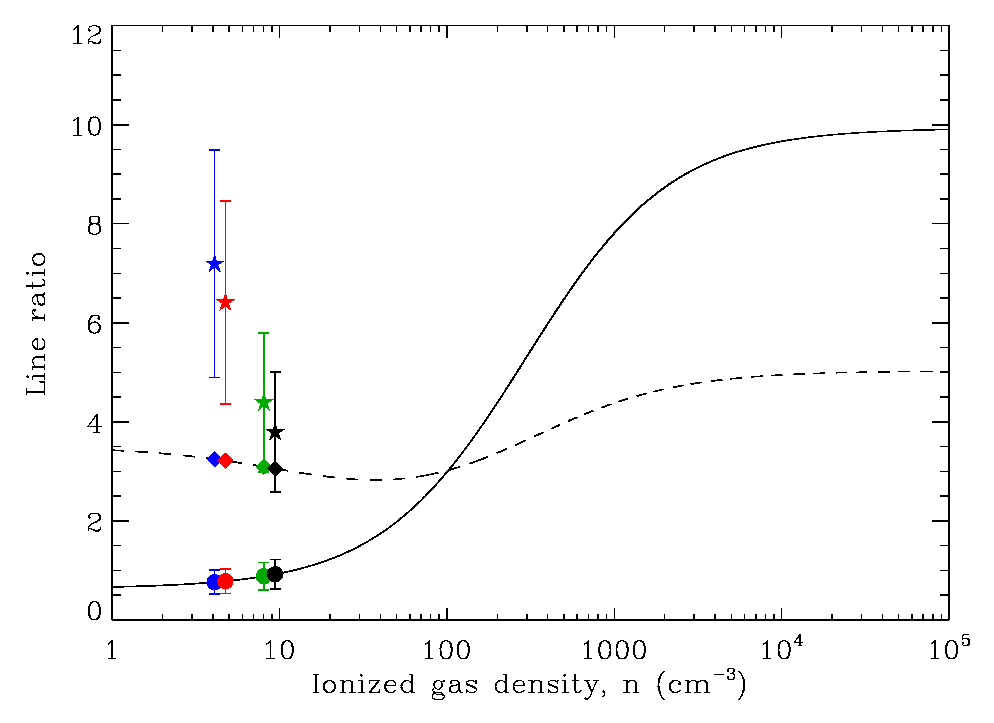
\includegraphics[width=\columnwidth]{ch3/Figure5}
\caption[Comparison of the average observed line ratio to the theoretical curves for each of the four regions we probe in M51]{Comparison of the average observed line ratio to the theoretical curves for each of the four regions we probe in M51.  The black solid line represents the theoretical curve for the [N\,\textsc{ii}]122/[N\,\textsc{ii}]205 line ratio, while the black dashed line represents the theoretical curve for the [C\,\textsc{ii}]/[N\,\textsc{ii}]205 line ratio.  The pixels from the nucleus, center, arm, and interarm regions are shown in black, green, red, and blue, respectively.  The solid dots show where the observed [N\,\textsc{ii}]122/[N\,\textsc{ii}]205 line ratios for each region fall on the theoretical curve, thus allowing us to determine the ionized gas density.  The diamonds (stars) show the theoretical (observed) values of the [C\,\textsc{ii}]/[N\,\textsc{ii}]205 line ratio at the inferred ionized gas density.  The error bars on the observed line ratios include calibration uncertainties.}
\label{fig:line_ratio_compare}
\end{figure}

\begin{landscape}
\begin{deluxetable}{lccccc}
\tabletypesize{\small}
\tablecolumns{6}
\tablecaption{[N\,\textsc{ii}] Line Ratios and Ionized Fraction of [C\,\textsc{ii}]\label{table:ratio_properties}}
\tablewidth{0pt}
\tablehead{
\colhead{Region} & \colhead{Observed} & \colhead{$n_{e}$\tablenotemark{a} (cm$^{-3}$)}
	& \colhead{Predicted} & \colhead{Observed} & \colhead{Ionized Fraction} \\
    & \colhead{$[$N\,\textsc{ii}]$_{122}$/[N\,\textsc{ii}]$_{205}$} &
    & \colhead{$[$C\,\textsc{ii}]$^{\mathrm{ionized}}_{158}$/[N\,\textsc{ii}]$_{205}$\tablenotemark{b}}
    & \colhead{$[$C\,\textsc{ii}]$_{158}$/[N\,\textsc{ii}]$_{205}$} & \colhead{of [C\,\textsc{ii}]}}
 \startdata
 Nucleus  & $0.9^{+0.3}_{-0.2}$ & $9^{+10}_{-7}$   & $3.1^{+0.3}_{-0.2}$ & $4 \pm 1$ & $0.8^{+0.2}_{-0.2}$ \\
 Center   & $0.9^{+0.3}_{-0.2}$ & $8^{+10}_{-6}$   & $3.1^{+0.3}_{-0.2}$ & $4 \pm 1$ & $0.7^{+0.3}_{-0.2}$ \\
 Arm      & $0.78^{+0.25}_{-0.08}$ & $5^{+8}_{-3}$ & $3.2^{+0.1}_{-0.2}$ & $6 \pm 2$ & $0.5^{+0.3}_{-0.2}$ \\
 Interarm & $0.76^{+0.24}_{-0.06}$ & $4^{+8}_{-2}$ & $3.2^{+0.1}_{-0.3}$ & $7 \pm 2$ & $0.5^{+0.2}_{-0.1}$ \\
 \enddata
 \tablecomments{These are average values for each of the four regions, and calibration uncertainties are included.}
 \tablenotetext{a}{Derived from [N\,\textsc{ii}]122/[N\,\textsc{ii}]205; see text.}
 \tablenotetext{b}{Derived from $n_{e}$ and theoretical prediction of [C\,\textsc{ii}]/[N\,\textsc{ii}]205 ratio in ionized gas; see text.}
\end{deluxetable}
\end{landscape}

\subsubsection{Ionized Gas Characteristics}
The fraction of N$^{+}$ originating from diffuse ionized gas versus that originating from H\textsc{ii}~regions has been discussed at length in the literature.  A set of models for H\,\textsc{ii} regions by \citet{1985ApJS...57..349R} and a later model by \citet{1994ApJ...420..772R} show that the ratio between the two [N\,\textsc{ii}] lines, [N\,\textsc{ii}]122/[N\,\textsc{ii}]205, varies from 3 for $n_{\mathrm{e}} \sim 100~\mathrm{cm}^{-3}$ to 10 for $n_{e} \gtrsim 10^{3}~\mathrm{cm}^{-3}$.  When $n_{e} \ll n_{\mathrm{critical}}$, the theoretical value for this ratio is 0.7 \citep{1991ApJ...381..200W,1994ApJ...434..587B}.  Observations of [N\,\textsc{ii}]122 and [N\,\textsc{ii}]205 in the Milky Way show that the [N\,\textsc{ii}]122/[N\,\textsc{ii}]205 falls between 1.0 and 1.6 \citep{1991ApJ...381..200W}.  Comparison between the observed and theoretical ratios implies that between 60\% and 87\% of the [N\,\textsc{ii}] emission in the Milky Way as measured with the \emph{Cosmic Background Explorer} comes from diffuse gas while the remainder comes from H\,\textsc{ii} regions with $n_{\mathrm{e}} \sim 100~\mathrm{cm}^{-3}$.  \citet{1994ApJ...434..587B} re-examine the data presented in \citet{1991ApJ...381..200W} and find [N\,\textsc{ii}]122/[N\,\textsc{ii}]205 = $0.9 \pm 0.1$ assuming a constant ratio, but also note that their data are better fit when the ratio is allowed to vary.  Our observations show that [N\,\textsc{ii}]122/[N\,\textsc{ii}]205 ranges between $0.76^{+0.24}_{-0.06}$ and $0.92^{+0.3}_{-0.2}$, thus approaching the theoretical lower limit of 0.7, implying that much of the ionized gas is diffuse.  Nonetheless, our mean values of the [N\,\textsc{ii}] line ratios are consistent with those of the Milky Way.

Our values for the fraction of [C\,\textsc{ii}] emission coming from PDRs are lower than those determined in other nearby galaxies, as well as previous calculations for M51.  Furthermore, a gradient in this fraction has not previously been observed in other galaxies and is an important result.  Given that we believe that the Seyfert nucleus is not the major source of gas excitation in the center (see Section~\ref{seyfert_influence}), the high fraction of ionized gas likely indicates that there are more massive stars per unit volume providing the ionizing photons.

The [N\,\textsc{ii}]205 line is difficult to detect, and so it is often necessary to rely on the [C\,\textsc{ii}]/[N\,\textsc{ii}]122 line ratio to determine the ionized gas fraction in the [C\,\textsc{ii}] emission.  This ratio requires knowledge about the density of the gas, which can sometimes be difficult to obtain.  However, in the absence of [N\,\textsc{ii}]205 observations it is often the best way to estimate the ionized gas contribution to the observed [C\,\textsc{ii}] emission.  \citet{2001ApJ...561..766M} used the [C\,\textsc{ii}]/[N\,\textsc{ii}]122 emission and the Galactic value of the [N\,\textsc{ii}]122/[N\,\textsc{ii}]205 ratio to estimate that about 50\% of the observed [C\,\textsc{ii}] emission in their sample of galaxies orginiated in PDRs, in agreement with our results for the arm and interarm regions.  However, \citet{2005A&A...441..961K} used a similar method to determine that 70\%--85\% of [C\,\textsc{ii}] emission comes from PDRs in M51 and M83.  This is a much higher value than what we determine using the [N\,\textsc{ii}]205 line for M51, especially in the center and nuclear regions, where we find that a large fraction of [C\,\textsc{ii}] emission is coming from ionized gas.  In both cases the correction was applied globally, but our results demonstrate that this method may not accurately correct the observed [C\,\textsc{ii}] emission and thus lead to incorrect results when comparing observations to PDR models.

The [O\,\textsc{iii}] line can also be used to probe the ionized gas.  One diagnostic used for high-redshift galaxies is the ratio [O\,\textsc{iii}]/[N\,\textsc{ii}]122.  \citet{2011ApJ...740L..29F} showed that this ratio can constrain the hardness of the UV radiation field as the ionization potentials of N and O$^{+}$ are 14.5 and 35~eV, respectively, while the [N\,\textsc{ii}]122 and [O\,\textsc{iii}] lines have critical densities of 310 and 510~cm$^{-3}$, respectively.  This means that the line ratio is relatively constant as a function of gas density.  If the emission arises from H\,\textsc{ii} regions, then the ratio gives an indication of the effective stellar temperature of the ionizing source(s).  If the emission comes from an AGN, particularly from the narrow-line region (NLR), the ratio indicates the value of the ionization parameter, $U$.  This parameter represents the photon density of the incident radiation field on a molecular cloud divided by the gas density of the cloud and gives an indication of the amount of dust absorbing the ionizing flux \citep{2003ApJ...594..758L,2009ApJ...701.1147A}.

In their Figure~1, \citet{2011ApJ...740L..29F} compare their observed [O\,\textsc{iii}]/ [N\,\textsc{ii}]122 line ratio to that predicted for H\,\textsc{ii} regions using the model of \citet{1985ApJS...57..349R}, as well as the ratio predicted for an NLR within an AGN using the model of \citet{2004ApJS..153....9G}. For their high-redshift galaxy, the ratio satisfies either model as well as a combination of the two.  We find that for the nucleus region of M51, which represents the area covered by the PACS point-spread function, the [O\,\textsc{iii}]/[N\,\textsc{ii}]122 ratio is $0.33 \pm 0.05$, while for the somewhat larger `center' region we measure $0.23 \pm 0.05$.  Following the method of \citet{2011ApJ...740L..29F}, we compare our observed ratios to model predictions.  Assuming that the emission is from an H\,\textsc{ii} region, our results suggest that the most luminous stars are B0 \citep{1996ApJ...460..914V} for both the nucleus and center regions.  On the other hand, if we assume that the emission is from the AGN, our results imply a small ionization parameter of $10^{-4}$ to $10^{-3.5}$, which means the incident ionizing flux is weak.  A comparison of our average [O\,\textsc{iii}]/$F_{\mathrm{TIR}}$ ratio to model predictions of the ratio for AGN and starburst galaxies from \citet{2009ApJ...701.1147A} shows that our ratio of $2\pm1$ is also consistent with a low value of $U$.  Furthermore, \citet{2004A&A...414..825S} conducted a survey of galaxies with low-luminosity nuclei using IRS LWS spectroscopy, including M51. They determined that the flux of the [O\,\textsc{iv}] line, which is only excited in AGNs due to the strong ionization potential of O$^{++}$ (55~eV), is lower in the nucleus of M51 than in typical AGNs.  This result also indicates weak activity in the nucleus of M51. Thus, we conclude that the Seyfert nucleus in M51 is not significantly affecting the excitation of the gas.

%%%%%%%%%%%%%%%%%%%%%%%%%%%%%%%%%%%%%%%%%%%%%%%%%%%%%%%%%%%%%%%%%%%

\section{PDR Modeling of Observations}\label{pdr_model3}
We compare our observed line ratios to the PDR model of \citet{1999ApJ...527..795K,2006ApJ...644..283K}.  This model probes PDRs with two free parameters, namely, the density of hydrogen nuclei, $n$, and the strength of the FUV radiation field incident on the PDR, $G_{0}$.  \citet{1999ApJ...527..795K} consider a density range of $10^{1}\,\mathrm{cm}^{-3} \le n \le 10^{7}\,\mathrm{cm}^{-3}$ and an FUV radiation field range of $10^{-0.5} \le G_{0} \le 10^{6.5}$.  Here we look at the inner part of M51 by carrying out a pixel-by-pixel comparison between the model and our observations and consider pixels within four regions, namely, the ``nucleus'', the ``center'', the ``arm,'' and the ``interarm'' regions.  These regions were distinguished using flux cutoffs in our total infrared flux map (Figure~\ref{fig:Ltir}) to isolate the nucleus from the rest of the center region and the spiral arms from the interarm regions.  Breaking the galaxy down into four distinct subregions allows us to probe the gas in different environments within the galaxy.  These regions are outlined in Figure~\ref{fig:regions} with cutoff maximum fluxes of $9.6 \times 10^{-7}$ and $3.7 \times 10^{-5}$~W~m$^{-2}$~sr$^{-1}$ for the interarm and arm regions, respectively.  The center region consists of everything above $3.7 \times 10^{-5}$~W~m$^{-2}$~sr$^{-1}$ except for the central nine pixels which comprise the nucleus.  We note that with a pixel scale of 4$\arcsec$ in our maps, each pixel is not independent from its neighbors.  In Table~\ref{table:flux_values} we list the average integrated intensity measured in each region for each of the five far-infrared lines that we have observed. 

\begin{figure}
\centering
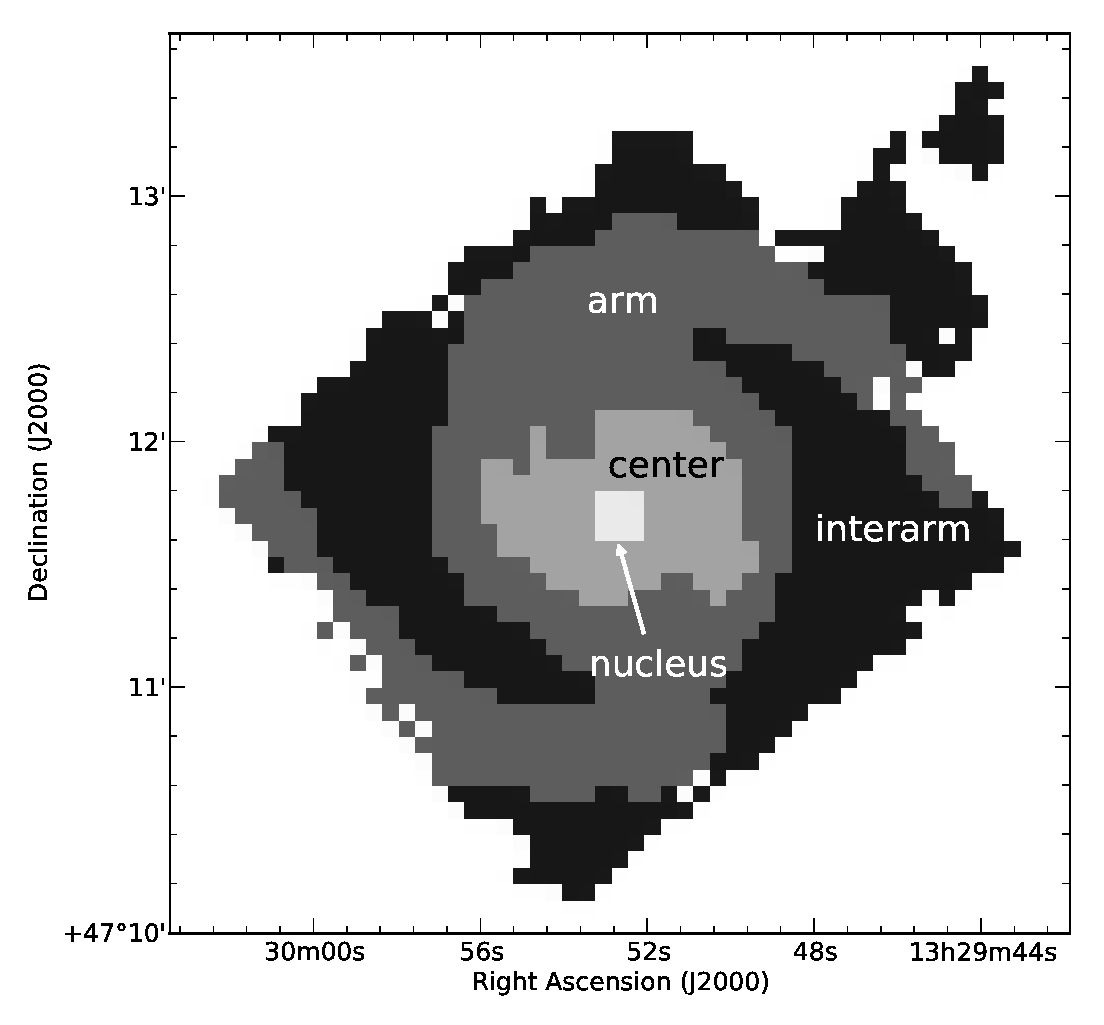
\includegraphics[width=\columnwidth]{ch3/Figure6}
\caption{Schematic of the four regions into which we divide M51 for our analysis.}
\label{fig:regions}
\end{figure}

\begin{landscape}
\begin{deluxetable}{lccccc}
\tabletypesize{\small}
\tablecolumns{6}
\tablecaption{Average Intensity of Fine-structure lines by Region\label{table:flux_values}}
\tablewidth{0pt}
\tablehead{
\colhead{Region} & \multicolumn{5}{c}{Integrated Intensity (W~m$^{-2}$~sr$^{-1}$)} \\
          & \colhead{[C\,\textsc{ii}](158~$\mu$m)} & \colhead{[N\,\textsc{ii}](122~$\mu$m)}
          & \colhead{[O\,\textsc{i}](63~$\mu$m)} & \colhead{[O\,\textsc{i}](145~$\mu$m)} & \colhead{[O\,\textsc{iii}](88~$\mu$m)}}
 \startdata
 Nucleus\tablenotemark{a}  & $(1.4 \pm 0.1) \times 10^{-8}$  & $(3.2 \pm 0.2) \times 10^{-9}$
 	& $(8 \pm 1) \times 10^{-9}$      & $(7 \pm 2) \times 10^{-10}$ & $(1.0 \pm 0.1) \times 10^{-9}$ \\
 Center\tablenotemark{b}   & $(1.1 \pm 0.2) \times 10^{-9}$  & $(1.7 \pm 0.4) \times 10^{-10}$
 	& $(2.9 \pm 0.7) \times 10^{-10}$ & $(3 \pm 1) \times 10^{-11}$ & $(8 \pm 2) \times 10^{-11}$ \\
 Arms\tablenotemark{c}     & $(1.2 \pm 0.5) \times 10^{-10}$ & $(1.4 \pm 0.9) \times 10^{-11}$
 	& $(3 \pm 1) \times 10^{-11}$     & $(4 \pm 1) \times 10^{-11}$ & $(8 \pm 2) \times 10^{-11}$ \\
 Interarm\tablenotemark{d} & $(5 \pm 2) \times 10^{-11}$     & $(8 \pm 3) \times 10^{-12}$
 	& $(1.8 \pm 0.5) \times 10^{-11}$ & $(3.2 \pm 0.8) \times 10^{-11}$ & $(1.7 \pm 0.4) \times 10^{-10}$ \\
 \enddata
 \tablecomments{Average integrated intensity measured in the four different regions for each of the far-infrared fine-structure lines, using our maps with a 5$\sigma$ cut applied.  The uncertainties shown are the standard deviations.}
 \tablenotetext{a}{The number of pixels included in this measurement is 9 for all five lines.}
 \tablenotetext{b}{The number of pixels included in this measurement is 136 for the [C\,\textsc{ii}], [N\,\textsc{ii}]122, and [O\,\textsc{i}]63 lines, 95 for the [O\,\textsc{i}]145 line, and 93 for the [O\,\textsc{iii}] line.}
 \tablenotetext{c}{The number of pixels included in this measurement is 583, 560, 553, 46, and 61 for the [C\,\textsc{ii}], [N\,\textsc{ii}]122, [O\,\textsc{i}]63, [O\,\textsc{i}]145, and [O\,\textsc{iii}] lines, respectively.}
 \tablenotetext{d}{The number of pixels included in this measurement is 607, 391, 394, 38, and 23 for the [C\,\textsc{ii}], [N\,\textsc{ii}]122, [O\,\textsc{i}]63, [O\,\textsc{i}]145, and [O\,\textsc{iii}] lines, respectively.}
\end{deluxetable}
\end{landscape}

In Figure~\ref{fig:CIIonOIvsCIIOIonLfir}(a) we show the [C\,\textsc{ii}]/[O\,\textsc{i}]63 ratio versus the ([C\,\textsc{ii}]+[O\,\textsc{i}]63)/$F_{\mathrm{TIR}}$ ratio for M51 overlaid on the parameter space defined by lines of constant log($n/\mathrm{cm}^{-3}$) (dotted lines) and log$G_{0}$ (solid lines) adapted from plots in \citet{1999ApJ...527..795K}.  The authors of that paper note that for extragalactic sources it is recommended that the observed total infrared flux be reduced by a factor of two to account for the (optically thin) infrared continuum flux coming from both the front and back sides of the cloud, whereas the model assumes that emission is only coming from the front side of the cloud, just as the fine-structure lines do.  Here we have applied this correction to our observed total infrared flux in order to compare it properly with the PDR model.  However, in this plot we have not yet corrected for the fraction of [C\,\textsc{ii}] emission arising from ionized gas (see Section~\ref{ionized_gas} for details).  We also note that the $F_{\mathrm{TIR}}$ we use for our comparison to the \citet{1999ApJ...527..795K} model is equivalent to their bolometric far-infrared flux.

\begin{figure}[!htbp]
 \subfloat[]{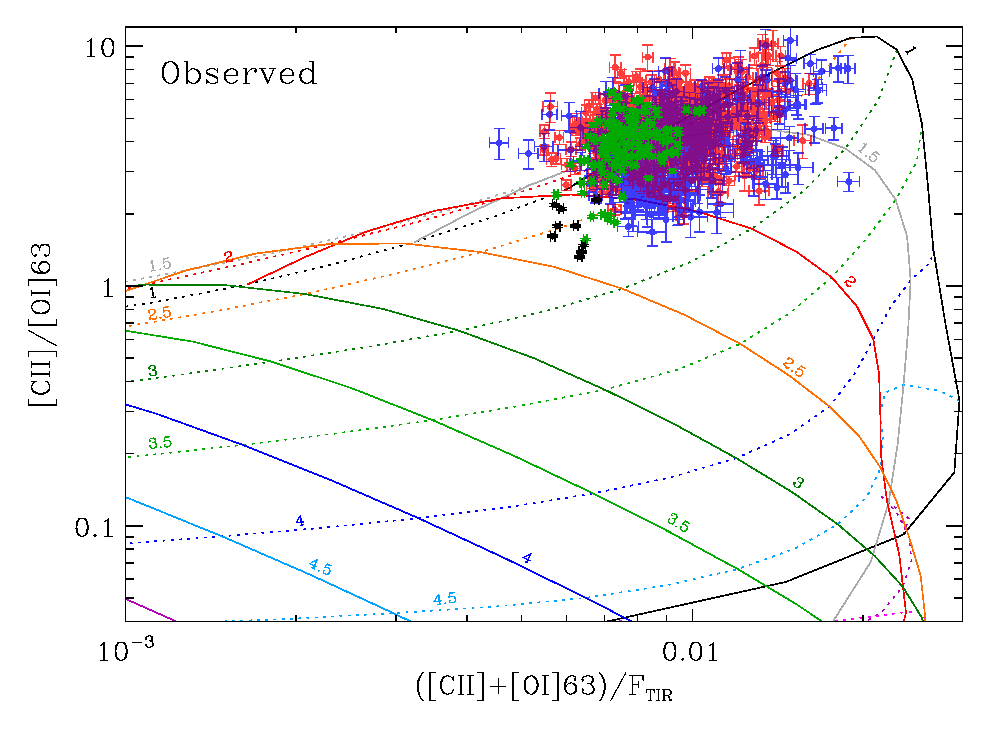
\includegraphics[width=\columnwidth]{ch3/Figure7a}}\\
\caption[Comparisons of observed line ratios in M51 with a PDR model grid using the uncorrected and corrected observations]{Our observed data are overlaid on the PDR model grid of lines of constant log($n/\mathrm{cm}^{-3}$) (dotted lines) and log$G_0$ (solid lines).  One data point represents one pixel.  The pixels from the nucleus, center, arm, and interarm regions are shown in black, green, red, and blue, respectively.  (a) [C\,\textsc{ii}]/[O\,\textsc{i}]63 vs. ([C\,\textsc{ii}]+[O\,\textsc{i}]63)/$F_{\mathrm{TIR}}$ prior to removing the fraction of [C\,\textsc{ii}] emission from ionized gas. (b) [C\,\textsc{ii}]/[O\,\textsc{i}]63 vs. ([C\,\textsc{ii}]+[O\,\textsc{i}]63)/F$_{\mathrm{TIR}}$ with the [C\,\textsc{ii}] emission corrected to remove the fraction originating in ionized gas, and the [O\,\textsc{i}]63 emission corrected for an ensemble of clouds (see text).}
\label{fig:CIIonOIvsCIIOIonLfir}
\end{figure}
\begin{figure}[!htbp]
\ContinuedFloat
\subfloat[]{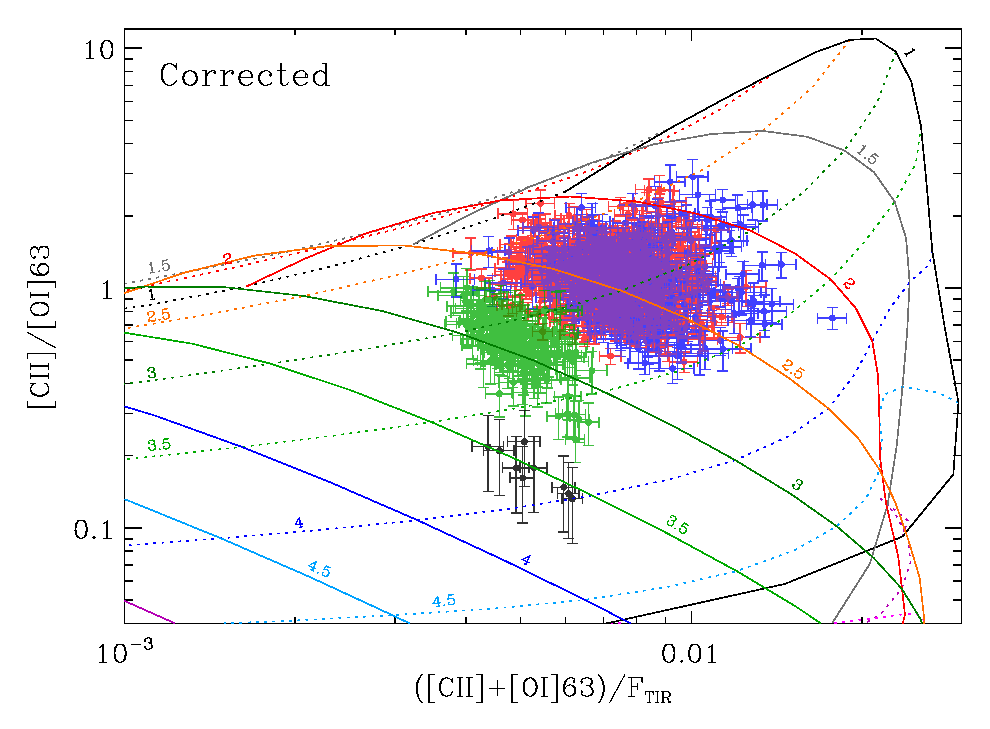
\includegraphics[width=\columnwidth]{ch3/Figure7b}}\\
\caption[]{\emph{continued}}
\end{figure}

With the exception of the nucleus, all of the data points tend to cluster around one locus and approximately one-third of the pixels fall outside of the parameter space covered by the models.  The [C\,\textsc{ii}]/[O\,\textsc{i}]63 versus ([C\,\textsc{ii}]+[O\,\textsc{i}]63)/$F_{\mathrm{TIR}}$ parameter space actually provides two possible model solutions.  One is a low-$G_0$, high-$n$ regime, and the other is a regime with more moderate values for both parameters.  We do not display the low-$G_0$, high-$n$ solutions as we can eliminate these solutions by considering the number of clouds emitting within our beam.  When we compare the model-predicted [C\,\textsc{ii}] emission based on the values of $G_0$ and $n$ to our observed [C\,\textsc{ii}] emission, we find that we would require a filling factor (i.e., the number of PDRs) of upward of $10^{3}$, which is an unreasonably large number of clouds along the line of sight.  This is the same reasoning used by \citet{2005A&A...441..961K} to eliminate the low-$G_0$, high-$n$ solution.  Thus, for the remaining discussion we consider only the moderate $n$ and $G_{0}$ solutions.

\subsection{Adjustments to the [C\,{\footnotesize II}] and [O\,{\footnotesize I}]63 Lines}\label{pdr_model_adjustments}
A proper comparison to the PDR model of \citet{1999ApJ...527..795K} requires us to make two adjustments.  The first is to remove the fraction of [C\,\textsc{ii}] emission from ionized gas, as the model only applies to [C\,\textsc{ii}] emission from PDRs.  We use the results from Section~\ref{ionized_gas_contribution} to correct our [C\,\textsc{ii}] map.

The second correction is applied to the [O\,\textsc{i}]63 map.  The \citet{1999ApJ...527..795K} model is a plane-parallel slab that only experiences an incident radiation field on one side, which is the same side from which we observe emission from the far-infrared cooling lines.  In the case of M51, there are many clouds within a given PACS beam, and the irradiated side of an individual cloud is not always oriented such that it is facing us.  \citet{1999ApJ...527..795K} caution that the velocity dispersion for such an ensemble of clouds, combined with the assumption that the [O\,\textsc{i}]63 line will become optically thick much faster than either the [C\,\textsc{ii}] line or the total infrared flux, means we observe only [O\,\textsc{i}]63 flux emitted from clouds with their front (lit) sides facing toward us, but we will observe [C\,\textsc{ii}] and total infrared flux from all clouds.  Thus, we only see about half of the total [O\,\textsc{i}]63 emission from all PDRs within our beam, and as a result we multiply the observed [O\,\textsc{i}]63 emission by a factor of two for comparison with the PDR model.

The resulting parameter space after the [C\,\textsc{ii}] and [O\,\textsc{i}]63 results have been corrected is shown in Figure~\ref{fig:CIIonOIvsCIIOIonLfir}(b), and the values for $n$ and $G_0$ are presented in Table~\ref{table:pdr_model_results}.  Comparing the two panels of Figure~\ref{fig:CIIonOIvsCIIOIonLfir}, we can see that after applying the appropriate corrections to the [C\,\textsc{ii}] and [O\,\textsc{i}]63 emission there is a general shift of pixels to lower values of ([C\,\textsc{ii}]+[O\,\textsc{i}]63)/$F_{\mathrm{TIR}}$.  In addition, pixels from the center and nuclear regions have decreased more in [C\,\textsc{ii}]/[O\,\textsc{i}]63, as expected.  Looking at Table~\ref{table:pdr_model_results}, we see an increase in $n$ by approximately an order of magnitude for all four regions after we apply our corrections. Likewise, log$G_0$ increases by $\sim$ 1.5.

% updated: February 26, 2013
\begin{deluxetable}{lccccc}
\tabletypesize{\small}
\tablecolumns{5}
\tablecaption{Properties of the Gas Derived from the PDR Model\label{table:pdr_model_results}}
\tablewidth{0pt}
\tablehead{
\colhead{Case} & \colhead{Region} & \colhead{log($n$/cm$^{-3}$)} & \colhead{log$G_{0}$}
	& \colhead{$T$ (K)}}
 \startdata
 Uncorrected\tablenotemark{a} & Nucleus  & 2.25--2.75  & 2.0--2.5    & 170--320 \\
             				  & Center   & 1.5--2.75   & 1.0--2.5    & 70--1070 \\
             				  & Arms     & 1.5--3.0    & 1.0--2.25   & 60--820  \\
             				  & Interarm & 1.5--3.25   & 0.75--2.25  & 50--820  \\
 \hline
 Corrected\tablenotemark{b}   & Nucleus  & 3.5--4.25   & 3.25--4.0   & 240--475 \\
             				  & Center   & 2.5--4.0    & 2.5--3.5    & 170--680 \\
             				  & Arms     & 2.0--3.75   & 1.75--3.0   & 100--760 \\
             				  & Interarm & 2.25--3.75  & 1.5--3.0    & 80--550  \\
 \enddata
 \tablenotetext{a}{The uncorrected case includes all of the observed [C\,\textsc{ii}] emission.}
 \tablenotetext{b}{The corrected case includes only [C\,\textsc{ii}] emission from neutral gas, and the [O\,\textsc{i}]63 has been increased by a factor of two as described in Section~\ref{pdr_model_adjustments}.}
\end{deluxetable}

We use our derived values for $n$ and $G_{0}$ to determine the range in the surface temperature of the gas using Figure~1 from \citet{1999ApJ...527..795K}.  The temperatures for the uncorrected [C\,\textsc{ii}] and [O\,\textsc{i}]63 observations, as well as for the full corrected case, are given in Table~\ref{table:pdr_model_results}.  In general, the cloud surface temperatures increase after the corrections are applied, while there is a decrease in temperature from the central region to the interarm region.

\subsection{Possible Contamination from the Seyfert Nucleus}\label{seyfert_influence}
The [O\,\textsc{i}]63 emission peaks in the nucleus of M51, and as a result [C\,\textsc{ii}]/[O\,\textsc{i}]63 is lower in the center than in the rest of the galaxy.  In addition, the [O\,\textsc{iii}] line is also brightest in the nucleus and center regions, thus indicating higher densities and warmer temperatures in the center of the galaxy.  This is consistent with the results of our PDR modeling, but it is also possible that some of the [O\,\textsc{i}]63 emission from the nucleus is not arising from starlight but rather from shock heating.  Once the temperature of the gas behind a shock front has cooled down to below 5000~K, the [O\,\textsc{i}]63 line dominates the cooling for densities below $10^{5}$~cm$^{-3}$ \citep{1989ApJ...342..306H}.  If indeed some of the [O\,\textsc{i}]63 emission did arise from shocks rather than stellar radiation in PDRs, then this correction would mean that the [C\,\textsc{ii}]/[O\,\textsc{i}]63 ratio attributable to PDRs would increase in the center of the galaxy. Thus, the data point(s) in Figure~\ref{fig:CIIonOIvsCIIOIonLfir} would shift upward and to the left in the parameter space, thus decreasing the gas density, and possibly the value of $G_{0}$ as well, although quantifying this effect would be difficult.  As a result, the gradient we observe in density and radiation field due to PDRs would become less prominent.  We also note here that some of the total infrared flux may originate in non-PDRs such as H\textsc{ii} regions.  Reducing this flux would move our data points to the right in Figure~\ref{fig:CIIonOIvsCIIOIonLfir}.

\subsection{Implications of PDR Model Results}
The range of densities, temperatures, and FUV radiation field strengths presented in Table~\ref{table:pdr_model_results} agree with the range of temperatures that we obtain for the [O\,\textsc{i}]63/[O\,\textsc{i}]145 line ratio if the [O\,\textsc{i}]63 line is optically thick ($T \gtrsim 200$~K).  In calculating these results, we have assumed that the corrections we applied to our observations of the fine-structure lines (i.e., removing the [C\,\textsc{ii}] emission originating from diffuse ionized gas and accounting for [O\,\textsc{i}]63 emission escaping away from our line of sight) and the total infrared flux (reducing the total observed flux by a factor of two to remove emission originating from the back side of or even beyond the cloud) are correct for comparing our observations to the PDR model.  However, it is possible that some of the remaining $F_{\mathrm{TIR}}$ emission originates from regions other than PDRs (such as H\,\textsc{ii} regions or the diffuse ISM), meaning less than half of the total observed flux comes from PDRs.  In such a case, the data points in the ``Corrected'' panel of Figure~\ref{fig:CIIonOIvsCIIOIonLfir} would shift to the right, thus resulting in lower values of $G_{0}$ and higher densities.  Looking at this figure, we see that we can only reduce the fraction of $F_{\mathrm{TIR}}$ originating in PDRs to approximately 1/8 of the total observed infrared flux before our data would no longer be consistent with the PDR model.  Thus, our data and analysis are consistent with at least 12\% and at most 50\% of $F_{\mathrm{TIR}}$ arising from PDRs in M51.

Our values of $n$ and $G_{0}$ are in good agreement with previous extragalactic surveys. Furthermore, our results agree with resolved studies of individual galaxies.  However, none of these studies show a decreasing trend with radius such as we show here, not only because of resolution constraints, but also because most previous work has not looked at variations with region within an individual galaxy.  \citet{2005A&A...441..961K} searched within the center of M51, as well as two positions in the spiral arms with \emph{ISO}; however, they were unable to resolve any differences between the three locations.

We see that the arm and interarm regions have approximately the same range of $G_{0}$ and $n$ despite lower star formation rate surface densities in the interarm region.  This may indicate that molecular clouds and star formation are similar in the arm and interarm regions, but there are just fewer clouds per unit area in the interarm regions.  To confirm this result, we have calculated the mean values of [C\,\textsc{ii}]/[O\,\textsc{i}]63 and ([C\,\textsc{ii}]+[O\,\textsc{i}]63)/$F_{\mathrm{TIR}}$ for each region and compared them to the PDR model.  The results are summarized in Table~\ref{table:pdr_model_result_mean}.  We also compare these results with surveys and individual galaxies in Table~\ref{pdr_comparison}.

\begin{deluxetable}{lcccc}
\tabletypesize{\small}
\tablecolumns{5}
\tablecaption{Properties of the Gas from the PDR Model and Mean Line Ratios\label{table:pdr_model_result_mean}}
\tablewidth{0pt}
\tablehead{
\colhead{Region}  & \colhead{Average\tablenotemark{a}} & \colhead{Average\tablenotemark{a}} & \colhead{log($n$/cm$^{-3}$)}
		& \colhead{log$G_{0}$} \\
                  & \colhead{($[\mathrm{C\,II}]+[\mathrm{O\,I}]$(63~$\mu$m))/$F_{\mathrm{TIR}}$}
  				  & \colhead{$[\mathrm{C\,II}]/[\mathrm{O\,I}]$(63~$\mu$m)} &  & }
 \startdata
 Nucleus  & $(5.3 \pm 0.2) \times 10^{-3}$   & $0.18 \pm 0.01$ & 3.75--4.0           & 3.25--3.75 \\
 Center   & $(5.01 \pm 0.05) \times 10^{-3}$ & $0.60 \pm 0.01$ & 3.0--3.25           & 2.75--3.0  \\
 Arms     & $(7.35 \pm 0.06) \times 10^{-3}$ & $1.18 \pm 0.01$ & 2.75--3.0           & 2.25--2.5  \\
 Interarm & $(8.10 \pm 0.09) \times 10^{-3}$ & $1.14 \pm 0.02$ & 2.75--3.0           & 2.25--2.5  \\
 \enddata
 \tablenotetext{a}{Uncertainties are the standard error for the means.  Calibration uncertainties are not included.}
\end{deluxetable}

\begin{deluxetable}{cccc}
\tabletypesize{\small}
\tablecolumns{4}
\tablecaption{Comparison of the PDR Characteristics Measured in M51 to Previous Studies\label{pdr_comparison}}
\tablewidth{0pt}
\tablehead{
\colhead{Paper} & \colhead{Source(s)} & \colhead{log($n$/cm$^{-3}$)} & \colhead{log$G_{0}$}}
 \startdata
 This work                   & Nucleus                 & 3.75--4.0   & 3.25--3.75 \\ 
 \nodata                     & Center                  & 3.0--3.25   & 2.75--3.0  \\
 \nodata                     & Arms                    & 2.75--3.0   & 2.25--2.5  \\
 \nodata                     & Interarm                & 2.75--3.0   & 2.25--2.5  \\
 (1) 						 & Normal galaxies         & 2.0--4.0    & 2.0--4.0   \\
 (2) 						 & AGN, starbursts, normal & 2.0--4.5    & 2.0--4.5   \\
 (3) 						 & NGC~5713                & 4.2        & 2.8       \\
 (4) 						 & NGC~4214                & 3.3--3.5    & 2.9--3.0   \\
 (5) 						 & NGC~6946, NGC~1313      & 2.0--4.0    & 2.0--4.0   \\
 (6) 						 & M83, M51                & 2.0--4.25   & 2.5--5.0   \\
 (7) 						 & NGC~1097, NGC~4559      & 2.5--3.0    & 1.7--3.0   \\
 (8)			 			 & M33 (BCLMP\,302) 	   & 2.5 		& 1.5 \\
 \enddata
 \tablerefs{(1) \citet{2001A&A...375..566N}; (2) \citet{2001ApJ...561..766M}; (3) \citet{1996A&A...315L.117L}; (4) \citet{2010A&A...518L..57C}; (5) \citet{2002AJ....124..751C}; (6) \citet{2005A&A...441..961K}; (7) \citet{2012ApJ...747...81C}; (8) \citet{2011A&A...532A.152M}.}
\end{deluxetable}

Finally, we compare our values for $G_{0}$ with those determined using other approaches.  First, assuming that all of our observed infrared flux has been converted from the impedent FUV flux by dust grains, we can compare the inferred values of $G_{0}$ from the PDR model to the observed $F_{\mathrm{TIR}}$ in M51.  To convert the observed integrated intensity of the TIR continuum we follow \citet{2005A&A...441..961K} and calculate $G_{0}^{\mathrm{obs}}$ as $4\pi I_{\mathrm{TIR}}^{\mathrm{slab}}/2(1.6 \times 10^{-3}$~erg~cm$^{-2}$~s$^{-1})$, where $I_{\mathrm{TIR}}^{\mathrm{slab}}$ is the observed total integrated intensity reduced by a factor of two, to consider only emission from the front side of the cloud, as described above.  We find mean values for $G_{0}^{\mathrm{obs}}$ of 120, 100, 35, and 15 for the nucleus, center, arm, and interarm regions, respectively, in fairly good agreement with those determined by \citet{2005A&A...441..961K}, who found values of roughly 76, 20, and 15 for the nucleus and two locations in the spiral arms of M51.  The ratio of the observed radiation field to that from the PDR model, $G_{0}^{\mathrm{obs}}$/$G_{0}$, gives us a filling factor for the clouds within each beam.  We find filling factors of roughly 2\%--7\%, 10\%--20\%, 10\%--20\%, and 4\%--8\% for the nucleus, center, arm, and interarm regions, respectively.  The lower filling factor in the interarm region is consistent with our theory that there are fewer clouds in this region than in the spiral arms.

Next, we compare the model-predicted values of $G_{0}$ to the value of the FUV field determined using dust SED modeling by \citet{2012ApJ...755..165M}.  They model the SED using the model of \citet{2007ApJ...657..810D}, which parameterizes the ISRF with $U$, a scaling factor of the average Milky Way ISRF spectrum, $U_{\mathrm{MW}}$ from \citet{1983A&A...128..212M}. We note here that the conversion between $U$ and $G_{0}$ is $U$ = 0.88$G_{0}$ \citep{2007ApJ...663..866D}.  The ambient ISRF is represented in the dust SED model by $U_{\mathrm{min}}$. In addition, the model has a ``PDR'' component that represents a stronger radiation field due to massive stars.  This component comprises a sum of intensities with $U$ scaling factors ranging between $U_{\mathrm{min}}$ and 10$^{6}U_{\mathrm{MW}}$.  \citet{2012ApJ...755..165M} find that the typical ISRF in M51 is $\sim$5 to 10 times that of the average value in the Milky Way, and their analysis covers the central region of the galaxy where we have mapped our fine-structure lines.  They also determined that the PDR component contributes at most about 2\% of the total radiation field within the same region.

Ideally, we would make a direct comparison between $G_{0}$ measured in this work and the total strength of the radiation field measured within the PDR component as measured by the dust SED model.  However, this value was not reported by \citet{2012ApJ...755..165M}.  But we do point out that the dust SED modeling suggests that only 2\% of the dust content is exposed to the strong PDR component, whereas we find that at least 12\% of the total dust continuum emission originates in PDRs.  This difference may arise due to the different concept of a PDR in each model.  The \citet{1999ApJ...527..795K} picture adopts a PDR as any region within the ISM where FUV photons have a significant effect on the chemistry in that region, which can include regions with weak (i.e., ambient) values of $G_{0}$ \citep{1985ApJ...291..722T}.  On the other hand, the dust SED model of \citet{2007ApJ...657..810D} assumes that the PDR component is exposed to a radiation field above the ambient field, and thus may overlook some PDRs as defined by the \citet{1999ApJ...527..795K} model.  Our models produce in some sense an average measure of $G_{0}$ over all regions within a single PACS beam (including regions with both low and high FUV radiation field strengths), and so perhaps it is not surprising that our measured values of $G_{0}$ are larger than the value of $U_{\mathrm{min}}$.

\section{Conclusions}\label{conclusions3}
We present new \emph{Herschel} PACS and SPIRE observations of the grand design spiral galaxy M51 of the important fine-structure lines [C\,\textsc{ii}](158~$\mu$m), [N\,\textsc{ii}](122 and 205~$\mu$m), [O\,\textsc{i}](63~$\mu$m), [O\,\textsc{i}](145~$\mu$m), and [O\,\textsc{iii}](88~$\mu$m).  We measure several diagnostic ratios, including [C\,\textsc{ii}]/$F_{\mathrm{TIR}}$, ([C\,\textsc{ii}]+[O\,\textsc{i}]63)/$F_{\mathrm{TIR}}$, [C\,\textsc{ii}]/[O\,\textsc{i}]63, and [O\,\textsc{i}]145/[O\,\textsc{i}]63.  We find a [C\,\textsc{ii}]/$F_{\mathrm{TIR}}$ ratio of $4 \times 10^{-3}$ on average, consistent with previous results for M51, as well as other nearby galaxies in various surveys and resolved studies.  Furthermore, we see a slight deficit in this ratio in the central region of M51 when compared to the surrounding environment, and the ([C\,\textsc{ii}]+[O\,\textsc{i}]63)/$F_{\mathrm{TIR}}$ ratio suggests reduced heating efficiency in these central regions.  We also find that the [N\,\textsc{ii}]122/[N\,\textsc{ii}]205 ratio indicates that diffuse ionized gas dominates these emission lines.

We divide the disk of M51 into four regions to conduct a pixel-by-pixel analysis in each region to investigate possible variations within the properties of the interstellar gas.  We determine that the fraction of ionized gas contributing to the total observed [C\,\textsc{ii}] emission is approximately 80\% in the nucleus of the galaxy and decreases to 50\% in the arm and interarm regions.  The [O\,\textsc{i}]145/[O\,\textsc{i}]63 ratio indicates that the [O\,\textsc{i}]63 line is optically thick in the inner region of M51.  We correct for both the [O\,\textsc{i}] optical depth and the ionized contribution to the [C\,\textsc{ii}] emission in our analysis.

We compare our observed line ratios in each region to the PDR model of \citet{1999ApJ...527..795K} and find that the incident FUV fluxes are $G_{0}\sim$ $10^{3.25}$--$10^{4.0}$, $10^{2.25}$--$10^{3.75}$, $10^{1.5}$--$10^{3.0}$, and $10^{1.5}$--$10^{4.0}$ for the nucleus, center, arm, and interarm regions, respectively.  The density of hydrogen nuclei, $n$, is $10^{3.5}$--$10^{4.25}$, $10^{2.5}$--$10^{4.0}$, $10^{2.0}$--$10^{3.75}$, and $10^{2.25}$--$10^{4.25}$~cm$^{-3}$ for the nucleus, center, arm, and interarm regions, respectively.  These derived values are similar to those previously seen in M51 on larger scales, as well as global results of numerous galaxies in surveys such as \citet{2001ApJ...561..766M}.

We show for the first time that both $G_{0}$ and $n$ decrease with increasing radius within M51.  Furthermore, we find that the arm and interarm regions, despite having different star formation rate surface densities and physical processes, show approximately the same incident FUV field and density within their molecular clouds.  Finally, our data and analysis suggest that PDRs contribute between 12\% and 50\% of the total infrared emission in M51.

\section*{Acknowledgments}
T.J.P. would like to extend her thanks to the anonymous referee for his/her constructive comments, which have contributed to strengthening our work.  The research of C.D.W. is supported by the Natural Sciences and Engineering Research Council of Canada and the Canadian Space Agency.  The research of V.L. is supported by a CEA/Marie Curie Eurotalents fellowship.  PACS has been developed by a consortium of institutes led by MPE (Germany) and including UVIE (Austria); KU Leuven, CSL, IMEC (Belgium); CEA, LAM (France); MPIA (Germany); INAF-IFSI/OAA/OAP/OAT, LENS, SISSA (Italy); IAC (Spain). This development has been supported by the funding agencies BMVIT (Austria), ESA-PRODEX (Belgium), CEA/CNES (France), DLR (Germany), ASI/INAF (Italy), and CICYT/MCYT (Spain).  SPIRE has been developed by a consortium of institutes led by Cardiff University (UK) and including Univ. Lethbridge (Canada); NAOC (China); CEA, LAM (France); IFSI, Univ. Padua (Italy); IAC (Spain); Stockholm Observatory (Sweden); Imperial College London, RAL, UCL-MSSL, UKATC, Univ. Sussex (UK); and Caltech, JPL, NHSC, Univ. Colorado (USA). This development has been supported by national funding agencies: CSA (Canada); NAOC (China); CEA, CNES, CNRS (France); ASI (Italy); MCINN (Spain); SNSB (Sweden); STFC and UKSA (UK); and NASA (USA).  HIPE is a joint development by the Herschel Science Ground Segment Consortium, consisting of ESA, the NASA Herschel Science Center, and the HIFI, PACS and SPIRE consortia.  The James Clerk Maxwell Telescope is operated by The Joint Astronomy Centre on behalf of the Science and Technology Facilities Council of the United Kingdom, the Netherlands Organisation for Scientific Research, and the National Research Council of Canada. This research has made use of the NASA/IPAC Extragalactic Database (NED), which is operated by the Jet Propulsion Laboratory, California Institute of Technology, under contract with the National Aeronautics and Space Administration.  This research made use of APLpy, an open-source plotting package for Python hosted at http://aplpy.github.com.

%% Commands to initiate bibliography:
\begin{thebibliography}{84}
\expandafter\ifx\csname natexlab\endcsname\relax\def\natexlab#1{#1}\fi

\bibitem[{{Abel} {et~al.}(2009){Abel}, {Dudley}, {Fischer}, {Satyapal}, \& {van
  Hoof}}]{2009ApJ...701.1147A}
{Abel}, N.~P., {Dudley}, C., {Fischer}, J., {Satyapal}, S., \& {van Hoof},
  P.~A.~M. 2009, \apj, 701, 1147

\bibitem[{{Aniano} {et~al.}(2011){Aniano}, {Draine}, {Gordon}, \&
  {Sandstrom}}]{2011PASP..123.1218A}
{Aniano}, G., {Draine}, B.~T., {Gordon}, K.~D., \& {Sandstrom}, K. 2011, \pasp,
  123, 1218

\bibitem[{{Asplund} {et~al.}(2009){Asplund}, {Grevesse}, {Sauval}, \&
  {Scott}}]{2009ARA&A..47..481A}
{Asplund}, M., {Grevesse}, N., {Sauval}, A.~J., \& {Scott}, P. 2009, \araa, 47,
  481

\bibitem[{{Beir{\~a}o} {et~al.}(2010){Beir{\~a}o}, {Armus}, {Appleton},
  {Smith}, {Croxall}, {Murphy}, {Dale}, {Helou}, {Kennicutt}, {Calzetti},
  {Bolatto}, {Brandl}, {Crocker}, {Draine}, {Dumas}, {Engelbracht}, {Gil de
  Paz}, {Gordon}, {Groves}, {Hao}, {Hinz}, {Hunt}, {Johnson}, {Koda}, {Krause},
  {Leroy}, {Meidt}, {Richer}, {Rix}, {Rahman}, {Roussel}, {Sandstrom},
  {Sauvage}, {Schinnerer}, {Skibba}, {Srinivasan}, {Walter}, {Warren},
  {Wilson}, {Wolfire}, \& {Zibetti}}]{2010A&A...518L..60B}
{Beir{\~a}o}, P., {Armus}, L., {Appleton}, P.~N., {et~al.} 2010, \aap, 518, L60

\bibitem[{{Beir{\~a}o} {et~al.}(2012){Beir{\~a}o}, {Armus}, {Helou},
  {Appleton}, {Smith}, {Croxall}, {Murphy}, {Dale}, {Draine}, {Wolfire},
  {Sandstrom}, {Aniano}, {Bolatto}, {Groves}, {Brandl}, {Schinnerer},
  {Crocker}, {Hinz}, {Rix}, {Kennicutt}, {Calzetti}, {Gil de Paz}, {Dumas},
  {Galametz}, {Gordon}, {Hao}, {Johnson}, {Koda}, {Krause}, {van der Laan},
  {Leroy}, {Li}, {Meidt}, {Meyer}, {Rahman}, {Roussel}, {Sauvage},
  {Srinivasan}, {Vigroux}, {Walter}, \& {Warren}}]{2012ApJ...751..144B}
{Beir{\~a}o}, P., {Armus}, L., {Helou}, G., {et~al.} 2012, \apj, 751, 144

\bibitem[{{Bendo} {et~al.}(2012){Bendo}, {Galliano}, \&
  {Madden}}]{2012MNRAS.423..197B}
{Bendo}, G.~J., {Galliano}, F., \& {Madden}, S.~C. 2012, \mnras, 423, 197

\bibitem[{{Bennett} {et~al.}(1994){Bennett}, {Fixsen}, {Hinshaw}, {Mather},
  {Moseley}, {Wright}, {Eplee}, {Gales}, {Hewagama}, {Isaacman}, {Shafer}, \&
  {Turpie}}]{1994ApJ...434..587B}
{Bennett}, C.~L., {Fixsen}, D.~J., {Hinshaw}, G., {et~al.} 1994, \apj, 434, 587

\bibitem[{{Blum} \& {Pradhan}(1992)}]{1992ApJS...80..425B}
{Blum}, R.~D., \& {Pradhan}, A.~K. 1992, \apjs, 80, 425

\bibitem[{{Braine} {et~al.}(2012){Braine}, {Gratier}, {Kramer}, {Israel}, {van
  der Tak}, {Mookerjea}, {Boquien}, {Tabatabaei}, {van der Werf}, \&
  {Henkel}}]{2012A&A...544A..55B}
{Braine}, J., {Gratier}, P., {Kramer}, C., {et~al.} 2012, \aap, 544, A55

\bibitem[{{Brauher} {et~al.}(2008){Brauher}, {Dale}, \&
  {Helou}}]{2008ApJS..178..280B}
{Brauher}, J.~R., {Dale}, D.~A., \& {Helou}, G. 2008, \apjs, 178, 280

\bibitem[{{Calzetti} {et~al.}(2005){Calzetti}, {Kennicutt}, {Bianchi},
  {Thilker}, {Dale}, {Engelbracht}, {Leitherer}, {Meyer}, {Sosey}, {Mutchler},
  {Regan}, {Thornley}, {Armus}, {Bendo}, {Boissier}, {Boselli}, {Draine},
  {Gordon}, {Helou}, {Hollenbach}, {Kewley}, {Madore}, {Martin}, {Murphy},
  {Rieke}, {Rieke}, {Roussel}, {Sheth}, {Smith}, {Walter}, {White}, {Yi},
  {Scoville}, {Polletta}, \& {Lindler}}]{2005ApJ...633..871C}
{Calzetti}, D., {Kennicutt}, Jr., R.~C., {Bianchi}, L., {et~al.} 2005, \apj,
  633, 871

\bibitem[{{Contursi} {et~al.}(2002){Contursi}, {Kaufman}, {Helou},
  {Hollenbach}, {Brauher}, {Stacey}, {Dale}, {Malhotra}, {Rubio}, {Rubin}, \&
  {Lord}}]{2002AJ....124..751C}
{Contursi}, A., {Kaufman}, M.~J., {Helou}, G., {et~al.} 2002, \aj, 124, 751

\bibitem[{{Contursi} {et~al.}(2013){Contursi}, {Poglitsch}, {Gr{\'a}cia
  Carpio}, {Veilleux}, {Sturm}, {Fischer}, {Verma}, {Hailey-Dunsheath}, {Lutz},
  {Davies}, {Gonz{\'a}lez-Alfonso}, {Sternberg}, {Genzel}, \&
  {Tacconi}}]{2013A&A...549A.118C}
{Contursi}, A., {Poglitsch}, A., {Gr{\'a}cia Carpio}, J., {et~al.} 2013, \aap,
  549, A118

\bibitem[{{Cormier} {et~al.}(2010){Cormier}, {Madden}, {Hony}, {Contursi},
  {Poglitsch}, {Galliano}, {Sturm}, {Doublier}, {Feuchtgruber}, {Galametz},
  {Geis}, {de Jong}, {Okumura}, {Panuzzo}, \& {Sauvage}}]{2010A&A...518L..57C}
{Cormier}, D., {Madden}, S.~C., {Hony}, S., {et~al.} 2010, \aap, 518, L57

\bibitem[{{Cormier} {et~al.}(2012){Cormier}, {Lebouteiller}, {Madden}, {Abel},
  {Hony}, {Galliano}, {Baes}, {Barlow}, {Cooray}, {De Looze}, {Galametz},
  {Karczewski}, {Parkin}, {R{\'e}my}, {Sauvage}, {Spinoglio}, {Wilson}, \&
  {Wu}}]{2012A&A...548A..20C}
{Cormier}, D., {Lebouteiller}, V., {Madden}, S.~C., {et~al.} 2012, \aap, 548,
  A20

\bibitem[{{Crawford} {et~al.}(1985){Crawford}, {Genzel}, {Townes}, \&
  {Watson}}]{1985ApJ...291..755C}
{Crawford}, M.~K., {Genzel}, R., {Townes}, C.~H., \& {Watson}, D.~M. 1985,
  \apj, 291, 755

\bibitem[{{Croxall} {et~al.}(2012){Croxall}, {Smith}, {Wolfire}, {Roussel},
  {Sandstrom}, {Draine}, {Aniano}, {Dale}, {Armus}, {Beir{\~a}o}, {Helou},
  {Bolatto}, {Appleton}, {Brandl}, {Calzetti}, {Crocker}, {Galametz}, {Groves},
  {Hao}, {Hunt}, {Johnson}, {Kennicutt}, {Koda}, {Krause}, {Li}, {Meidt},
  {Murphy}, {Rahman}, {Rix}, {Sauvage}, {Schinnerer}, {Walter}, \&
  {Wilson}}]{2012ApJ...747...81C}
{Croxall}, K.~V., {Smith}, J.~D., {Wolfire}, M.~G., {et~al.} 2012, \apj, 747,
  81

\bibitem[{{Dale} \& {Helou}(2002)}]{2002ApJ...576..159D}
{Dale}, D.~A., \& {Helou}, G. 2002, \apj, 576, 159

\bibitem[{{Draine} \& {Li}(2007)}]{2007ApJ...657..810D}
{Draine}, B.~T., \& {Li}, A. 2007, \apj, 657, 810

\bibitem[{{Draine} {et~al.}(2007)}]{2007ApJ...663..866D}
{Draine}, B.~T., {et~al.} 2007, \apj, 663, 866

\bibitem[{{Ferkinhoff} {et~al.}(2011){Ferkinhoff}, {Brisbin}, {Nikola},
  {Parshley}, {Stacey}, {Phillips}, {Falgarone}, {Benford}, {Staguhn}, \&
  {Tucker}}]{2011ApJ...740L..29F}
{Ferkinhoff}, C., {Brisbin}, D., {Nikola}, T., {et~al.} 2011, \apjl, 740, L29

\bibitem[{{Galavis} {et~al.}(1997){Galavis}, {Mendoza}, \&
  {Zeippen}}]{1997A&AS..123..159G}
{Galavis}, M.~E., {Mendoza}, C., \& {Zeippen}, C.~J. 1997, \aaps, 123, 159

\bibitem[{{Galavis} {et~al.}(1998){Galavis}, {Mendoza}, \&
  {Zeippen}}]{1998A&AS..131..499G}
---. 1998, \aaps, 131, 499

\bibitem[{{Garnett} {et~al.}(2004){Garnett}, {Edmunds}, {Henry}, {Pagel}, \&
  {Skillman}}]{2004AJ....128.2772G}
{Garnett}, D.~R., {Edmunds}, M.~G., {Henry}, R.~B.~C., {Pagel}, B.~E.~J., \&
  {Skillman}, E.~D. 2004, \aj, 128, 2772

\bibitem[{{Garnett} {et~al.}(1999){Garnett}, {Shields}, {Peimbert},
  {Torres-Peimbert}, {Skillman}, {Dufour}, {Terlevich}, \&
  {Terlevich}}]{1999ApJ...513..168G}
{Garnett}, D.~R., {Shields}, G.~A., {Peimbert}, M., {et~al.} 1999, \apj, 513,
  168

\bibitem[{{Graci{\'a}-Carpio} {et~al.}(2008){Graci{\'a}-Carpio},
  {Garc{\'{\i}}a-Burillo}, {Planesas}, {Fuente}, \&
  {Usero}}]{2008A&A...479..703G}
{Graci{\'a}-Carpio}, J., {Garc{\'{\i}}a-Burillo}, S., {Planesas}, P., {Fuente},
  A., \& {Usero}, A. 2008, \aap, 479, 703

\bibitem[{{Graci{\'a}-Carpio} {et~al.}(2011){Graci{\'a}-Carpio}, {Sturm},
  {Hailey-Dunsheath}, {Fischer}, {Contursi}, {Poglitsch}, {Genzel},
  {Gonz{\'a}lez-Alfonso}, {Sternberg}, {Verma}, {Christopher}, {Davies},
  {Feuchtgruber}, {de Jong}, {Lutz}, \& {Tacconi}}]{2011ApJ...728L...7G}
{Graci{\'a}-Carpio}, J., {Sturm}, E., {Hailey-Dunsheath}, S., {et~al.} 2011,
  \apjl, 728, L7

\bibitem[{{Griffin} {et~al.}(2010)}]{2010A&A...518L...3G}
{Griffin}, M.~J., {et~al.} 2010, \aap, 518, L3

\bibitem[{{Groves} {et~al.}(2004){Groves}, {Dopita}, \&
  {Sutherland}}]{2004ApJS..153....9G}
{Groves}, B.~A., {Dopita}, M.~A., \& {Sutherland}, R.~S. 2004, \apjs, 153, 9

\bibitem[{{Habing}(1968)}]{1968BAN....19..421H}
{Habing}, H.~J. 1968, \bain, 19, 421

\bibitem[{{Ho} {et~al.}(1997){Ho}, {Filippenko}, \&
  {Sargent}}]{1997ApJS..112..315H}
{Ho}, L.~C., {Filippenko}, A.~V., \& {Sargent}, W.~L.~W. 1997, \apjs, 112, 315

\bibitem[{{Hollenbach} \& {McKee}(1989)}]{1989ApJ...342..306H}
{Hollenbach}, D., \& {McKee}, C.~F. 1989, \apj, 342, 306

\bibitem[{{Hollenbach} {et~al.}(1991){Hollenbach}, {Takahashi}, \&
  {Tielens}}]{1991ApJ...377..192H}
{Hollenbach}, D.~J., {Takahashi}, T., \& {Tielens}, A.~G.~G.~M. 1991, \apj,
  377, 192

\bibitem[{{Hudson} \& {Bell}(2004)}]{2004MNRAS.348.1275H}
{Hudson}, C.~E., \& {Bell}, K.~L. 2004, \mnras, 348, 1275

\bibitem[{{Kaufman} {et~al.}(2006){Kaufman}, {Wolfire}, \&
  {Hollenbach}}]{2006ApJ...644..283K}
{Kaufman}, M.~J., {Wolfire}, M.~G., \& {Hollenbach}, D.~J. 2006, \apj, 644, 283

\bibitem[{{Kaufman} {et~al.}(1999){Kaufman}, {Wolfire}, {Hollenbach}, \&
  {Luhman}}]{1999ApJ...527..795K}
{Kaufman}, M.~J., {Wolfire}, M.~G., {Hollenbach}, D.~J., \& {Luhman}, M.~L.
  1999, \apj, 527, 795

\bibitem[{{Kennicutt} {et~al.}(2003){Kennicutt}, {Armus}, {Bendo}, {Calzetti},
  {Dale}, {Draine}, {Engelbracht}, {Gordon}, {Grauer}, {Helou}, {Hollenbach},
  {Jarrett}, {Kewley}, {Leitherer}, {Li}, {Malhotra}, {Regan}, {Rieke},
  {Rieke}, {Roussel}, {Smith}, {Thornley}, \& {Walter}}]{2003PASP..115..928K}
{Kennicutt}, Jr., R.~C., {Armus}, L., {Bendo}, G., {et~al.} 2003, \pasp, 115,
  928

\bibitem[{{Kramer} {et~al.}(2005){Kramer}, {Mookerjea}, {Bayet},
  {Garcia-Burillo}, {Gerin}, {Israel}, {Stutzki}, \&
  {Wouterloot}}]{2005A&A...441..961K}
{Kramer}, C., {Mookerjea}, B., {Bayet}, E., {et~al.} 2005, \aap, 441, 961

\bibitem[{{Kramer} {et~al.}(2013){Kramer}, {Abreu-Vicente},
  {Garc{\'{\i}}a-Burillo}, {Rela{\~n}o}, {Aalto}, {Boquien}, {Braine},
  {Buchbender}, {Gratier}, {Israel}, {Nikola}, {R{\"o}llig}, {Verley}, {van der
  Werf}, \& {Xilouris}}]{2013A&A...553A.114K}
{Kramer}, C., {Abreu-Vicente}, J., {Garc{\'{\i}}a-Burillo}, S., {et~al.} 2013,
  \aap, 553, A114

\bibitem[{{Le Petit} {et~al.}(2006){Le Petit}, {Nehm{\'e}}, {Le Bourlot}, \&
  {Roueff}}]{2006ApJS..164..506L}
{Le Petit}, F., {Nehm{\'e}}, C., {Le Bourlot}, J., \& {Roueff}, E. 2006, \apjs,
  164, 506

\bibitem[{{Lebouteiller} {et~al.}(2012){Lebouteiller}, {Cormier}, {Madden},
  {Galliano}, {Indebetouw}, {Abel}, {Sauvage}, {Hony}, {Contursi}, {Poglitsch},
  {R{\'e}my}, {Sturm}, \& {Wu}}]{2012A&A...548A..91L}
{Lebouteiller}, V., {Cormier}, D., {Madden}, S.~C., {et~al.} 2012, \aap, 548,
  A91

\bibitem[{{Liseau} {et~al.}(2006){Liseau}, {Justtanont}, \&
  {Tielens}}]{2006A&A...446..561L}
{Liseau}, R., {Justtanont}, K., \& {Tielens}, A.~G.~G.~M. 2006, \aap, 446, 561

\bibitem[{{Lord} {et~al.}(1996){Lord}, {Malhotra}, {Lim}, {Helou}, {Rubin},
  {Stacey}, {Hollenbach}, {Werner}, {Thronson}, {Beichman}, {Dinerstein},
  {Hunter}, {Lo}, \& {Lu}}]{1996A&A...315L.117L}
{Lord}, S.~D., {Malhotra}, S., {Lim}, T., {et~al.} 1996, \aap, 315, L117

\bibitem[{{Luhman} {et~al.}(1997){Luhman}, {Jaffe}, {Sternberg}, {Herrmann}, \&
  {Poglitsch}}]{1997ApJ...482..298L}
{Luhman}, M.~L., {Jaffe}, D.~T., {Sternberg}, A., {Herrmann}, F., \&
  {Poglitsch}, A. 1997, \apj, 482, 298

\bibitem[{{Luhman} {et~al.}(2003){Luhman}, {Satyapal}, {Fischer}, {Wolfire},
  {Sturm}, {Dudley}, {Lutz}, \& {Genzel}}]{2003ApJ...594..758L}
{Luhman}, M.~L., {Satyapal}, S., {Fischer}, J., {et~al.} 2003, \apj, 594, 758

\bibitem[{{Luhman} {et~al.}(1998){Luhman}, {Satyapal}, {Fischer}, {Wolfire},
  {Cox}, {Lord}, {Smith}, {Stacey}, \& {Unger}}]{1998ApJ...504L..11L}
---. 1998, \apjl, 504, L11

\bibitem[{{Malhotra} {et~al.}(1997){Malhotra}, {Helou}, {Stacey}, {Hollenbach},
  {Lord}, {Beichman}, {Dinerstein}, {Hunter}, {Lo}, {Lu}, {Rubin},
  {Silbermann}, {Thronson}, \& {Werner}}]{1997ApJ...491L..27M}
{Malhotra}, S., {Helou}, G., {Stacey}, G., {et~al.} 1997, \apjl, 491, L27

\bibitem[{{Malhotra} {et~al.}(2001){Malhotra}, {Kaufman}, {Hollenbach},
  {Helou}, {Rubin}, {Brauher}, {Dale}, {Lu}, {Lord}, {Stacey}, {Contursi},
  {Hunter}, \& {Dinerstein}}]{2001ApJ...561..766M}
{Malhotra}, S., {Kaufman}, M.~J., {Hollenbach}, D., {et~al.} 2001, \apj, 561,
  766

\bibitem[{{Marble} {et~al.}(2010){Marble}, {Engelbracht}, {van Zee}, {Dale},
  {Smith}, {Gordon}, {Wu}, {Lee}, {Kennicutt}, {Skillman}, {Johnson}, {Block},
  {Calzetti}, {Cohen}, {Lee}, \& {Schuster}}]{2010ApJ...715..506M}
{Marble}, A.~R., {Engelbracht}, C.~W., {van Zee}, L., {et~al.} 2010, \apj, 715,
  506

\bibitem[{{Mathis} {et~al.}(1983){Mathis}, {Mezger}, \&
  {Panagia}}]{1983A&A...128..212M}
{Mathis}, J.~S., {Mezger}, P.~G., \& {Panagia}, N. 1983, \aap, 128, 212

\bibitem[{{Mentuch Cooper} {et~al.}(2012){Mentuch Cooper}, {Wilson}, {Foyle},
  {Bendo}, {Koda}, {Baes}, {Boquien}, {Boselli}, {Ciesla}, {Cooray}, {Eales},
  {Galametz}, {Lebouteiller}, {Parkin}, {Roussel}, {Sauvage}, {Spinoglio}, \&
  {Smith}}]{2012ApJ...755..165M}
{Mentuch Cooper}, E., {Wilson}, C.~D., {Foyle}, K., {et~al.} 2012, \apj, 755,
  165

\bibitem[{{Mookerjea} {et~al.}(2011){Mookerjea}, {Kramer}, {Buchbender},
  {Boquien}, {Verley}, {Rela{\~n}o}, {Quintana-Lacaci}, {Aalto}, {Braine},
  {Calzetti}, {Combes}, {Garcia-Burillo}, {Gratier}, {Henkel}, {Israel},
  {Lord}, {Nikola}, {R{\"o}llig}, {Stacey}, {Tabatabaei}, {van der Tak}, \&
  {van der Werf}}]{2011A&A...532A.152M}
{Mookerjea}, B., {Kramer}, C., {Buchbender}, C., {et~al.} 2011, \aap, 532, A152

\bibitem[{{Moustakas} {et~al.}(2010){Moustakas}, {Kennicutt}, {Tremonti},
  {Dale}, {Smith}, \& {Calzetti}}]{2010ApJS..190..233M}
{Moustakas}, J., {Kennicutt}, Jr., R.~C., {Tremonti}, C.~A., {et~al.} 2010,
  \apjs, 190, 233

\bibitem[{{Negishi} {et~al.}(2001){Negishi}, {Onaka}, {Chan}, \&
  {Roellig}}]{2001A&A...375..566N}
{Negishi}, T., {Onaka}, T., {Chan}, K.-W., \& {Roellig}, T.~L. 2001, \aap, 375,
  566

\bibitem[{{Nikola} {et~al.}(2001){Nikola}, {Geis}, {Herrmann}, {Madden},
  {Poglitsch}, {Stacey}, \& {Townes}}]{2001ApJ...561..203N}
{Nikola}, T., {Geis}, N., {Herrmann}, F., {et~al.} 2001, \apj, 561, 203

\bibitem[{{Oberst} {et~al.}(2006){Oberst}, {Parshley}, {Stacey}, {Nikola},
  {L{\"o}hr}, {Harnett}, {Tothill}, {Lane}, {Stark}, \&
  {Tucker}}]{2006ApJ...652L.125O}
{Oberst}, T.~E., {Parshley}, S.~C., {Stacey}, G.~J., {et~al.} 2006, \apjl, 652,
  L125

\bibitem[{{Ott}(2010)}]{2010ASPC..434..139O}
{Ott}, S. 2010, in Astronomical Society of the Pacific Conference Series, Vol.
  434, Astronomical Data Analysis Software and Systems XIX, ed. {Y.~Mizumoto,
  K.-I.~Morita, \& M.~Ohishi}, 139--+

\bibitem[{{Pilbratt} {et~al.}(2010)}]{2010A&A...518L...1P}
{Pilbratt}, G.~L., {et~al.} 2010, \aap, 518, L1

\bibitem[{{Poglitsch} {et~al.}(2010)}]{2010A&A...518L...2P}
{Poglitsch}, A., {et~al.} 2010, \aap, 518, L2

\bibitem[{{Pound} \& {Wolfire}(2008)}]{2008ASPC..394..654P}
{Pound}, M.~W., \& {Wolfire}, M.~G. 2008, in Astronomical Society of the
  Pacific Conference Series, Vol. 394, Astronomical Data Analysis Software and
  Systems XVII, ed. R.~W. {Argyle}, P.~S. {Bunclark}, \& J.~R. {Lewis}, 654

\bibitem[{{R{\"o}llig} {et~al.}(2006){R{\"o}llig}, {Ossenkopf}, {Jeyakumar},
  {Stutzki}, \& {Sternberg}}]{2006A&A...451..917R}
{R{\"o}llig}, M., {Ossenkopf}, V., {Jeyakumar}, S., {Stutzki}, J., \&
  {Sternberg}, A. 2006, \aap, 451, 917

\bibitem[{{R{\"o}llig} {et~al.}(2007){R{\"o}llig}, {Abel}, {Bell}, {Bensch},
  {Black}, {Ferland}, {Jonkheid}, {Kamp}, {Kaufman}, {Le Bourlot}, {Le Petit},
  {Meijerink}, {Morata}, {Ossenkopf}, {Roueff}, {Shaw}, {Spaans}, {Sternberg},
  {Stutzki}, {Thi}, {van Dishoeck}, {van Hoof}, {Viti}, \&
  {Wolfire}}]{2007A&A...467..187R}
{R{\"o}llig}, M., {Abel}, N.~P., {Bell}, T., {et~al.} 2007, \aap, 467, 187

\bibitem[{{Rubin}(1985)}]{1985ApJS...57..349R}
{Rubin}, R.~H. 1985, \apjs, 57, 349

\bibitem[{{Rubin} {et~al.}(1994){Rubin}, {Simpson}, {Lord}, {Colgan},
  {Erickson}, \& {Haas}}]{1994ApJ...420..772R}
{Rubin}, R.~H., {Simpson}, J.~P., {Lord}, S.~D., {et~al.} 1994, \apj, 420, 772

\bibitem[{{Satyapal} {et~al.}(2004){Satyapal}, {Sambruna}, \&
  {Dudik}}]{2004A&A...414..825S}
{Satyapal}, S., {Sambruna}, R.~M., \& {Dudik}, R.~P. 2004, \aap, 414, 825

\bibitem[{{Savage} \& {Sembach}(1996)}]{1996ARA&A..34..279S}
{Savage}, B.~D., \& {Sembach}, K.~R. 1996, \araa, 34, 279

\bibitem[{{Schinnerer} {et~al.}(2013){Schinnerer}, {Meidt}, {Pety}, {Hughes},
  {Colombo}, {Garcia-Burillo}, {Schuster}, {Dumas}, {Dobbs}, {Leroy}, {Kramer},
  {Thompson}, \& {Regan}}]{2013arXiv1304.1801S}
{Schinnerer}, E., {Meidt}, S.~E., {Pety}, J., {et~al.} 2013, ArXiv e-prints

\bibitem[{{Schirm} {et~al.}(2013){Schirm}, {Wilson}, {Parkin}, {Kamenetzky},
  {Glenn}, {Rangwala}, {Spinoglio}, {Pereira-Santaella}, {Baes}, {Barlow},
  {Clements}, {Cooray}, {De Looze}, {Madden}, {Remy}, \&
  {Wu}}]{Schirm_2013_submitted}
{Schirm}, M.~R.~P., {Wilson}, C.~D., {Parkin}, T.~J., {et~al.} 2013, \apj,
  submitted

\bibitem[{{Smith} {et~al.}(2007){Smith}, {Draine}, {Dale}, {Moustakas},
  {Kennicutt}, {Helou}, {Armus}, {Roussel}, {Sheth}, {Bendo}, {Buckalew},
  {Calzetti}, {Engelbracht}, {Gordon}, {Hollenbach}, {Li}, {Malhotra},
  {Murphy}, \& {Walter}}]{2007ApJ...656..770S}
{Smith}, J.~D.~T., {Draine}, B.~T., {Dale}, D.~A., {et~al.} 2007, \apj, 656,
  770

\bibitem[{{Spinoglio} {et~al.}(2012){Spinoglio}, {Dasyra}, {Franceschini},
  {Gruppioni}, {Valiante}, \& {Isaak}}]{2012ApJ...745..171S}
{Spinoglio}, L., {Dasyra}, K.~M., {Franceschini}, A., {et~al.} 2012, \apj, 745,
  171

\bibitem[{{Stacey} {et~al.}(1993){Stacey}, {Jaffe}, {Geis}, {Grenzel},
  {Harris}, {Poglitsch}, {Stutzki}, \& {Townes}}]{1993ApJ...404..219S}
{Stacey}, G.~J., {Jaffe}, D.~T., {Geis}, N., {et~al.} 1993, \apj, 404, 219

\bibitem[{{Stacey} {et~al.}(1985){Stacey}, {Viscuso}, {Fuller}, \&
  {Kurtz}}]{1985ApJ...289..803S}
{Stacey}, G.~J., {Viscuso}, P.~J., {Fuller}, C.~E., \& {Kurtz}, N.~T. 1985,
  \apj, 289, 803

\bibitem[{{Sternberg} \& {Dalgarno}(1989)}]{1989ApJ...338..197S}
{Sternberg}, A., \& {Dalgarno}, A. 1989, \apj, 338, 197

\bibitem[{{Sternberg} \& {Dalgarno}(1995)}]{1995ApJS...99..565S}
---. 1995, \apjs, 99, 565

\bibitem[{{St{\"o}rzer} {et~al.}(2000){St{\"o}rzer}, {Zielinsky}, {Stutzki}, \&
  {Sternberg}}]{2000A&A...358..682S}
{St{\"o}rzer}, H., {Zielinsky}, M., {Stutzki}, J., \& {Sternberg}, A. 2000,
  \aap, 358, 682

\bibitem[{{Swinyard} {et~al.}(2010){Swinyard}, {Ade}, {Baluteau}, {Aussel},
  {Barlow}, {Bendo}, {Benielli}, {Bock}, {Brisbin}, {Conley}, {Conversi},
  {Dowell}, {Dowell}, {Ferlet}, {Fulton}, {Glenn}, {Glauser}, {Griffin},
  {Griffin}, {Guest}, {Imhof}, {Isaak}, {Jones}, {King}, {Leeks}, {Levenson},
  {Lim}, {Lu}, {Makiwa}, {Naylor}, {Nguyen}, {Oliver}, {Panuzzo},
  {Papageorgiou}, {Pearson}, {Pohlen}, {Polehampton}, {Pouliquen},
  {Rigopoulou}, {Ronayette}, {Roussel}, {Rykala}, {Savini}, {Schulz},
  {Schwartz}, {Shupe}, {Sibthorpe}, {Sidher}, {Smith}, {Spencer}, {Trichas},
  {Triou}, {Valtchanov}, {Wesson}, {Woodcraft}, {Xu}, {Zemcov}, \&
  {Zhang}}]{2010A&A...518L...4S}
{Swinyard}, B.~M., {Ade}, P., {Baluteau}, J.-P., {et~al.} 2010, \aap, 518, L4

\bibitem[{{Tielens} \& {Hollenbach}(1985)}]{1985ApJ...291..722T}
{Tielens}, A.~G.~G.~M., \& {Hollenbach}, D. 1985, \apj, 291, 722

\bibitem[{{Tikhonov} {et~al.}(2009){Tikhonov}, {Galazutdinova}, \&
  {Tikhonov}}]{2009AstL...35..599T}
{Tikhonov}, N.~A., {Galazutdinova}, O.~A., \& {Tikhonov}, E.~N. 2009, Astronomy
  Letters, 35, 599

\bibitem[{{Vacca} {et~al.}(1996){Vacca}, {Garmany}, \&
  {Shull}}]{1996ApJ...460..914V}
{Vacca}, W.~D., {Garmany}, C.~D., \& {Shull}, J.~M. 1996, \apj, 460, 914

\bibitem[{{van Dishoeck} \& {Black}(1986)}]{1986ApJS...62..109V}
{van Dishoeck}, E.~F., \& {Black}, J.~H. 1986, \apjs, 62, 109

\bibitem[{{van Dishoeck} \& {Black}(1988)}]{1988ApJ...334..771V}
---. 1988, \apj, 334, 771

\bibitem[{{Wolfire} {et~al.}(1990){Wolfire}, {Tielens}, \&
  {Hollenbach}}]{1990ApJ...358..116W}
{Wolfire}, M.~G., {Tielens}, A.~G.~G.~M., \& {Hollenbach}, D. 1990, \apj, 358,
  116

\bibitem[{{Wright} {et~al.}(1991){Wright}, {Mather}, {Bennett}, {Cheng},
  {Shafer}, {Fixsen}, {Eplee}, {Isaacman}, {Read}, {Boggess}, {Gulkis},
  {Hauser}, {Janssen}, {Kelsall}, {Lubin}, {Meyer}, {Moseley}, {Murdock},
  {Silverberg}, {Smoot}, {Weiss}, \& {Wilkinson}}]{1991ApJ...381..200W}
{Wright}, E.~L., {Mather}, J.~C., {Bennett}, C.~L., {et~al.} 1991, \apj, 381,
  200

\bibitem[{{Zubko} {et~al.}(2004){Zubko}, {Dwek}, \&
  {Arendt}}]{2004ApJS..152..211Z}
{Zubko}, V., {Dwek}, E., \& {Arendt}, R.~G. 2004, \apjs, 152, 211

\end{thebibliography}


%\bibliographystyle{apj}
%\bibliography{ch3/M51_bib} 


%\end{document}






\include{Ch4/ch4}
\pagestyle{fancy}
\headheight 20pt
\lhead{Ph.D. Thesis --- T.~J. Parkin}
\rhead{McMaster - Physics \& Astronomy}
\chead{}
\lfoot{}
\cfoot{\thepage}
\rfoot{}
\renewcommand{\headrulewidth}{0.1pt}
\renewcommand{\footrulewidth}{0.1pt}

\chapter{Summary \& Future Work} \label{chapter5}
\thispagestyle{fancy}

In this thesis I have utilised the unprecedented sensitivity and resolution of the \emph{Herschel Space Observatory}, designed to probe the cold interstellar medium (ISM) from roughly 55 to 672~$\mu$m using both photometric and spectroscopic instruments.  Our goal was to search for local variations within the ISM of two contrasting environments, namely the nearby galaxies Centaurus~A (Cen~A) and M51.  In addition, I strived to contribute to the overall understanding of the effects of an active galactic nucleus (AGN) to the neighbouring ISM.  Lastly, I wanted to characterise the nature of the disk of Cen~A to establish if it warrants the `peculiar' designation it has received in its morphological classification.

In Chapter~\ref{chapter2} I focused on the cold gas and dust in Cen~A using \emph{Herschel} PACS and SPIRE observations of the dust continuum at 70, 160, 250, 350 and 500~$\mu$m.  I combined these data with observations of the CO($J=3-2$) transition from the HARP-B instrument on the James Clerk Maxwell Telescope to obtain measurements of the molecular gas content of the warped disk.  Using a modified blackbody I modelled the dust spectral energy distribution (SED) on a pixel-by-pixel basis with the \emph{Herschel} photometry and found a radial decrease in both the dust temperature, varying from 30~K down to 20~K, as well as the dust mass distribution.  Furthermore, I found a similar radial distribution in the total gas distribution.  Most interestingly, however, when I created a map of the gas-to-dust mass ratio I found a radial trend in this as well.  While the average value I found of $103 \pm 8$ is consistent with that of the Milky Way, the region in the vicinity of the AGN had a gas-to-dust ratio of almost 275.  Eliminating a gradient in the metallicity or the CO($J=3-2$)/CO($J=1-0$) ratio as possible explanations for this trend, I concluded that the AGN is removing dust from the surrounding ISM via dust sputtering by a hard X-ray radiation field or dust expulsion by the jets.  Thus, in the case of Cen~A I have found that indeed the AGN does have an effect on the neighbouring regions.

Next, I turned to the grand-design spiral galaxy M51 and presented \emph{Herschel} spectroscopy of the central $2.5\arcmin \times 2.5\arcmin$ of the disk in Chapter~\ref{chapter3}.  These observations targeted the important far-infrared fine-structure lines [C~\textsc{ii}](158~$\mu$m), [N~\textsc{ii}](122 \& 205~$\mu$m), [O~\textsc{i}](63 \& 145~$\mu$m) and [O~\textsc{iii}](88~$\mu$m), which are the dominant contributors to the global gas cooling budget in both neutral and ionised phases, particularly in photon dominated (photodissociation) regions (PDRs) and H~\textsc{ii} regions.  I subdivided our maps into four distinct regions, namely the nucleus (which contains a Seyfert~2 nucleus), centre, arm and interarm regions, to search for trends in the physical characteristics of the gas.  I determined for the first time that there is a radial trend in the contribution to the [C~\textsc{ii}](158~$\mu$m) emission from ionised gas, from 80\% in the nucleus down to about 50\% in the arm and interarm regions.  Furthermore, I found a slight suppression in the heating efficiency in the nucleus compared to the other regions, as shown by a decrease in the ([C~\textsc{ii}](158~$\mu$m)+[O~\textsc{i}](63~$\mu$m))/$F_{\mathrm{TIR}}$ ratio with increasing 70~$\mu$m/160~$\mu$m colour.  A comparison between our spectroscopy and a PDR model revealed a decreasing trend in the strength of the far-ultraviolet radiation field, $G_{0}$ and density of hydrogen nuclei, $n$, as a function of increasing radius (or region).  For the first time I also show that there is no difference in $G_{0}$ and $n$ between the arm and interarm regions, despite having different star formation rate densities.  This in turn, indicates that there is no difference in the molecular cloud properties between those in the spiral arms of M51, and those in the interarm regions.  Again I have shown that an active nucleus affects the ISM in the surrounding region.

Lastly, in Chapter~\ref{chapter4} I examine a radial strip of the eastern half of the disk in Cen~A in the same cooling lines I investigated in M51.  I divided the strip into eight bins to deduce any radial trends in the gas component of the ISM, as I found in M51 in Chapter~\ref{chapter2}.  I found that there is a slight trend with increasing radius in the heating efficiency, as it is reduced near the nucleus by about a factor of two compared to larger radii.  I also determined that, unlike M51, the majority of the [C~\textsc{ii}](158~$\mu$m) emission originates in neutral gas.  Futhermore, I also do not observe any significant radial changes in the values of $G_{0}$ and $n$.  However, the most significant result of this investigation is that the values of $G_{0}$ and $n$ are more consistent with normal spiral galaxies than elliptical galaxies.  Thus, while Cen~A is a typical elliptical galaxy on global scales, its disk exhibits properties of a spiral galaxy with an active nucleus.

There are a few implications of the results of this thesis on the evolution of the ISM in general.  A reduction in the heating efficiency has been attributed to the dust grains and polycyclic aromatic hydrocarbons becoming too positively charged to efficiently free electrons, which in turn, contribute to gas heating \citep{1985ApJ...291..722T,2012ApJ...747...81C,2012A&A...548A..91L}.  I observe such a decrease in the nuclei of both M51 and Cen~A, though in Cen~A it is slightly less obvious.  This would imply that the active nuclei of both sources are impacting the  heating and cooling processes in the gas, which ultimately will lead to a reduction in the gas's ability to cool enough to form molecular cores and the next generation of stars.

My results in Chapter~\ref{chapter3} and Chapter~\ref{chapter4} demonstrate that molecular clouds possess similar properties regardless of whether they are in the arms or interarm regions.  Ultimately, this result would imply that the reason the spiral arms appear more prominent in disk galaxies is simply due to an increase in the number of molecular clouds producing young stars that, in turn, contribute to heating the gas and dust.  Perhaps molecular clouds are also very similar in nature in all galaxies producing stars, and this is something I can look into by studying other nearby galaxies.

\subsection{Future Work}\label{future}
To further solidify our conclusions that active galactic nuclei directly affect the surrounding ISM, I would like to extend our investigation to other nearby galaxies.  In particular, it would be ideal to probe sources with varying AGN luminosities to see if their impact on the ISM changes with luminosity.  A couple of potential options are NGC~4151 and NGC~1068.  Both of these galaxies have been observed with \emph{Herschel} as part of the Very Nearby Galaxies Survey.  In addition, I have obtained CO($J=3-2$) observations from the JCMT, revealing detections in CO($J=3-2$) for NGC~1068, but interestingly, I only determined an upper limit for NGC~4151.  A previous study of NGC~1068 by \citet{2012ApJ...758..108S} used the SPIRE FTS instrument to study the CO ladder and determined there is an X-ray dominated region likely influenced by the AGN.  We can expand on this work to fully probe the surrounding ISM.  NGC~4151 is an interesting target because we do not observe CO($J=3-2$), thus suggesting there is very little warm molecular gas in it; however, it has been detected in CO($J=1-0$) \citep{2010ApJ...721..911D}.  It has a Seyfert~1 nucleus \citep{2000A&ARv..10..135U} and is classified as a barred spiral \citep{1991trcb.book.....D}.  Thus, this galaxy would give us yet another unique perspective on AGN impact on the ISM.

Another potential direction we can take is to expand our PDR region modelling to other galaxies to further characterise the molecular cloud properties.  One way to definitively explain the subtle differences we see between Cen~A and M51 is to investigate a target that is fully edge on, such as NGC~891.  This galaxy is classified as an SAb morphological type \citep{1991trcb.book.....D}, and is located about 9.6~Mpc away \citep{2004ApJS..151..193S}, giving us the same spatial resolution as M51.  It is believed to be a close analogue to the Milky Way, and its orientation allows for in-depth studies of the disk and the halo \citep{1984A&A...140..470V,1993ApJ...404L..59S,2009MNRAS.395...97W}.  It has also been well studied at numerous wavelengths \citep[e.g.][]{1993ApJ...404L..59S,2009MNRAS.395...97W,2011A&A...531L..11B,2013ApJ...762...12H}.  Recently, \citet{2013ApJ...766...57B} studied the gas in the halo 5~kpc above the plane and determined from its metallicity that it was  from the disk via a galactic fountain.  These properties make it an interesting target for conducting further PDR analysis.

We have spectroscopic observations of a radial strip along one half of the disk of NGC~891 in the same important cooling lines as we have just presented for M51 and Cen~A from PACS and SPIRE.  A similar analysis into NGC~891 could aid in interpreting our results in Chapters~\ref{chapter3} and \ref{chapter4}, and determine if the slight difference in $G_{0}$ and $n$ between the two galaxies is an inclination effect.  

Lastly, I can propose to observe Cen~A with the Atacama Large Millimetre Array (ALMA) to aid in contraining our PDR model results.  ALMA will be able to observe Cen~A at unprecedented resolution in the submillimetre, giving us access to the CO($J=3-2$) line and its adjacent dust continuum on spatial scales of less than 1.0--1.4$\arcsec$ \citep{alma_primer}, corresponding to physical scales of less than approximately 26~pc at the distance of Cen~A.  At these scales, we can resolve individual giant molecular clouds with masses larger than roughly $10^{4}$~M$_{\odot}$, and possibly resolve the nucleus, which is still point-source like in a 2.4$\arcsec \times 6\arcsec$ beam \citep{2009ApJ...695..116E}.

It is crucial to take advantage of infrared and submillimetre observations of nearby galaxies to help us fully understand the life cycle of the ISM and the impact of star formation on its host molecular cloud.  Now that the \emph{Herschel Space Observatory} has ended its observing lifetime, we need to fully exploit the data it has produced and continue to probe the local properties of the dust and gas in nearby galaxies.  If we can understand the evolution of the ISM we can improve our understanding on galaxy evolution as a whole.  This thesis has presented important results that aid in bringing us closer to this goal.

%\bibliography{thesis_bib}
%\bibliographystyle{apj}

\begin{thebibliography}{17}
\expandafter\ifx\csname natexlab\endcsname\relax\def\natexlab#1{#1}\fi

\bibitem[{{Bianchi} \& {Xilouris}(2011)}]{2011A&A...531L..11B}
{Bianchi}, S., \& {Xilouris}, E.~M. 2011, \aap, 531, L11

\bibitem[{{Bregman} {et~al.}(2013){Bregman}, {Miller}, {Seitzer}, {Cowley}, \&
  {Miller}}]{2013ApJ...766...57B}
{Bregman}, J.~N., {Miller}, E.~D., {Seitzer}, P., {Cowley}, C.~R., \& {Miller},
  M.~J. 2013, \apj, 766, 57

\bibitem[{{Croxall} {et~al.}(2012){Croxall}, {Smith}, {Wolfire}, {Roussel},
  {Sandstrom}, {Draine}, {Aniano}, {Dale}, {Armus}, {Beir{\~a}o}, {Helou},
  {Bolatto}, {Appleton}, {Brandl}, {Calzetti}, {Crocker}, {Galametz}, {Groves},
  {Hao}, {Hunt}, {Johnson}, {Kennicutt}, {Koda}, {Krause}, {Li}, {Meidt},
  {Murphy}, {Rahman}, {Rix}, {Sauvage}, {Schinnerer}, {Walter}, \&
  {Wilson}}]{2012ApJ...747...81C}
{Croxall}, K.~V., {Smith}, J.~D., {Wolfire}, M.~G., {et~al.} 2012, \apj, 747,
  81

\bibitem[{{de Vaucouleurs} {et~al.}(1991){de Vaucouleurs}, {de Vaucouleurs},
  {Corwin}, {Buta}, {Paturel}, \& {Fouque}}]{1991trcb.book.....D}
{de Vaucouleurs}, G., {de Vaucouleurs}, A., {Corwin}, Jr., H.~G., {et~al.}
  1991, {Third Reference Catalogue of Bright Galaxies} (Springer-Verlag, New
  York)

\bibitem[{{Dumas} {et~al.}(2010){Dumas}, {Schinnerer}, \&
  {Mundell}}]{2010ApJ...721..911D}
{Dumas}, G., {Schinnerer}, E., \& {Mundell}, C.~G. 2010, \apj, 721, 911

\bibitem[{{Espada} {et~al.}(2009){Espada}, {Matsushita}, {Peck}, {Henkel},
  {Iono}, {Israel}, {Muller}, {Petitpas}, {Pihlstr{\"o}m}, {Taylor}, \&
  {Dinh-V-Trung}}]{2009ApJ...695..116E}
{Espada}, D., {Matsushita}, S., {Peck}, A., {et~al.} 2009, \apj, 695, 116

\bibitem[{{Hodges-Kluck} \& {Bregman}(2013)}]{2013ApJ...762...12H}
{Hodges-Kluck}, E.~J., \& {Bregman}, J.~N. 2013, \apj, 762, 12

\bibitem[{{Lebouteiller} {et~al.}(2012){Lebouteiller}, {Cormier}, {Madden},
  {Galliano}, {Indebetouw}, {Abel}, {Sauvage}, {Hony}, {Contursi}, {Poglitsch},
  {R{\'e}my}, {Sturm}, \& {Wu}}]{2012A&A...548A..91L}
{Lebouteiller}, V., {Cormier}, D., {Madden}, S.~C., {et~al.} 2012, \aap, 548,
  A91
  
\bibitem[\protect\citeauthoryear{ALMA Primer}{2012}]{alma_primer}
  {Schieven}, G., ed., 2012, Observing with ALMA: A Primer for Early Science, ALMA Doc. 		1.1, ver. 1.1

\bibitem[{{Scoville} {et~al.}(1993){Scoville}, {Thakkar}, {Carlstrom}, \&
  {Sargent}}]{1993ApJ...404L..59S}
{Scoville}, N.~Z., {Thakkar}, D., {Carlstrom}, J.~E., \& {Sargent}, A.~I. 1993,
  \apjl, 404, L59

\bibitem[{{Spinoglio} {et~al.}(2012){Spinoglio}, {Pereira-Santaella},
  {Busquet}, {Schirm}, {Wilson}, {Glenn}, {Kamenetzky}, {Rangwala}, {Maloney},
  {Parkin}, {Bendo}, {Madden}, {Wolfire}, {Boselli}, {Cooray}, \&
  {Page}}]{2012ApJ...758..108S}
{Spinoglio}, L., {Pereira-Santaella}, M., {Busquet}, G., {et~al.} 2012, \apj,
  758, 108

\bibitem[{{Strickland} {et~al.}(2004){Strickland}, {Heckman}, {Colbert},
  {Hoopes}, \& {Weaver}}]{2004ApJS..151..193S}
{Strickland}, D.~K., {Heckman}, T.~M., {Colbert}, E.~J.~M., {Hoopes}, C.~G., \&
  {Weaver}, K.~A. 2004, \apjs, 151, 193

\bibitem[{{Struve} {et~al.}(2010){Struve}, {Oosterloo}, {Morganti}, \&
  {Saripalli}}]{2010A&A...515A..67S}
{Struve}, C., {Oosterloo}, T.~A., {Morganti}, R., \& {Saripalli}, L. 2010,
  \aap, 515, A67+

\bibitem[{{Tielens} \& {Hollenbach}(1985)}]{1985ApJ...291..722T}
{Tielens}, A.~G.~G.~M., \& {Hollenbach}, D. 1985, \apj, 291, 722

\bibitem[{{Ulrich}(2000)}]{2000A&ARv..10..135U}
{Ulrich}, M.-H. 2000, \aapr, 10, 135

\bibitem[{{van der Kruit}(1984)}]{1984A&A...140..470V}
{van der Kruit}, P.~C. 1984, \aap, 140, 470

\bibitem[{{Whaley} {et~al.}(2009){Whaley}, {Irwin}, {Madden}, {Galliano}, \&
  {Bendo}}]{2009MNRAS.395...97W}
{Whaley}, C.~H., {Irwin}, J.~A., {Madden}, S.~C., {Galliano}, F., \& {Bendo},
  G.~J. 2009, \mnras, 395, 97

\end{thebibliography}



\label{lastpage}

%\end{singlespace}
\end{doublespace}


%%%%%%%%%%%%%%%%%%%%%%%%%%%%%%%%%%%%%%%%%%%%%%%%%%%%%%%%%%%%%%%
%Appendices
%%%%%%%%%%%%%%%%%%%%%%%%%%%%%%%%%%%%%%%%%%%%%%%%%%%%%%%%%%%%%%%
%\appendix
%\include{Appendix-A/Appendix-A}
%\include{Appendix-B/Appendix-B}


%%%%%%%%%%%%%%%%%%%%%%%%%%%%%%%%%%%%%%%%%%%%%%%%%%%%%%%%%%%%%%%
% ESM students need to include a Nontechnical Abstract as the %
% last appendix.                                              %
%%%%%%%%%%%%%%%%%%%%%%%%%%%%%%%%%%%%%%%%%%%%%%%%%%%%%%%%%%%%%%%
% This \include command should point to the file containing
% that abstract.
%\include{nontechnical-abstract}
%%%%%%%%%%%%%%%%%%%%%%%%%%%%%%%%%%%%%%%%%%%
% End of the \allowdisplaybreak command %
%%%%%%%%%%%%%%%%%%%%%%%%%%%%%%%%%%%%%%%%%%%



%%%%%%%%%%%%%%%%
% BIBLIOGRAPHY %
%%%%%%%%%%%%%%%% 
% You can use BibTeX or other bibliography facility for your
% bibliography. LaTeX's standard stuff is shown below. If you
% bibtex, then this section should look something like:
\begin{singlespace}
  
  \pagestyle{fancy}
  \headheight 20pt
  \lhead{Ph.D. Thesis --- T.~J. Parkin}
  \rhead{McMaster - Physics and Astronomy}
  \chead{}
  \lfoot{}
  \cfoot{\thepage}
  \rfoot{}
  \renewcommand{\headrulewidth}{0.1pt}
  \renewcommand{\footrulewidth}{0.1pt}
  \thispagestyle{fancy}
  
  %\bibliography{thesis_bib}
  %\bibliographystyle{apj}
%  \nocite{*}
  
  \addcontentsline{toc}{chapter}{Bibliography}
  
  \thispagestyle{fancy}
  
\end{singlespace}


\end{document}
